\def\thudbabelopt{italian,english}
\documentclass[target=mst,aauheader=,style=]{thud}

\course{Computer Science}
\title{Detecting Routing Failures in LLM-based Multi-Agent Systems through Linear Probes}
\author{Andrea Cantarutti}
\supervisor{Prof.\ Giorgio Brajnik}
\cosupervisor{Prof.\ Kevin Roitero}

\usepackage[a-2b]{pdfx}
\usepackage[numbers]{natbib}
\usepackage{booktabs}
\usepackage{tabularx}
\usepackage{float}
\usepackage{placeins}
\usepackage{tikz}
\usetikzlibrary{arrows.meta, positioning}
\usepackage[most]{tcolorbox}
\usepackage{colortbl}
\usepackage[normalem]{ulem}
\definecolor{bindingcolor}{RGB}{0,90,156}
\definecolor{waivedcolor}{RGB}{180,80,0}
\definecolor{omegaSmall}{RGB}{214,234,248}
\definecolor{omegaMedium}{RGB}{133,193,233}
\definecolor{omegaLarge}{RGB}{41,128,185}
\newcommand{\binding}[1]{{\color{bindingcolor}\uline{#1}}}
\newcommand{\waived}[1]{\textcolor{waivedcolor}{#1}}
\newcommand{\subA}[1]{\textcolor{bindingcolor}{#1}}
\newcommand{\subB}[1]{\textcolor{waivedcolor}{#1}}
\newcommand{\best}[1]{\textbf{#1}}
\newcommand{\worst}[1]{\uline{#1}}
\newtcolorbox{problembox}[1][Problem]{%
  colback=white, colframe=black, boxrule=0.5pt, arc=0pt,
  left=8pt, right=8pt, top=7pt, bottom=7pt,
  before upper={\bfseries\sffamily\small #1\par\vspace{3pt}\hrule\vspace{6pt}\normalfont\normalsize}
}
\newtcolorbox{scenariobox}[1]{%
  colback=white, colframe=black, boxrule=0.5pt, arc=0pt,
  left=8pt, right=8pt, top=7pt, bottom=7pt,
  before upper={\bfseries\sffamily\small #1\par\vspace{3pt}\hrule\vspace{6pt}\normalfont\normalsize}
}
\newtcolorbox{rqbox}[1][RQ]{%
  colback=white, colframe=black, boxrule=0.5pt, arc=0pt,
  left=8pt, right=8pt, top=7pt, bottom=7pt,
  before upper={\bfseries\sffamily\small #1\par\vspace{3pt}\hrule\vspace{6pt}\normalfont\normalsize\itshape}
}
\newtcolorbox{quotebox}{%
  colback=white, colframe=white, boxrule=0pt, arc=0pt,
  borderline west={2pt}{0pt}{black},
  left=14pt, right=8pt, top=6pt, bottom=6pt,
  fontupper=\itshape
}
\usepackage{fancyvrb}
\usepackage{fvextra}
\DefineVerbatimEnvironment{promptverbatim}{Verbatim}{%
  fontsize=\small, breaklines=true, breakanywhere=true, breaksymbolleft={},
  frame=single, framesep=2.5mm, rulecolor=\color{black!60},
}
\usepackage[pdfa]{hyperref}
\hypersetup{
  colorlinks=true,
  linkcolor=black,
  citecolor=black,
  urlcolor=black,
  filecolor=black,
}

\begin{document}
\maketitle

\begin{dedication}
As your future \\
becomes my past, \\
eternally \\
we converge. \\
\end{dedication}

\acknowledgements
I would like to express my gratitude to Professor Giorgio Brajnik and Professor Kevin Roitero, for their precious guidance and support throughout the development of this work.

I would also like to thank all my friends and colleagues, my lifelong companion Rachele, my mother Clara, and my father Dario, to whom this work is dedicated.

\chapter+*{AI Usage Disclosure}
This statement covers the preparation of this work's text and code, not the use of large language models as part of the experimental method, which is described in the relevant chapters as an object of study.

During the preparation of this work, generative AI tools (Anthropic's Claude Sonnet 5 and Claude Opus 5) were used for the following purposes:

\begin{itemize}
  \item language polishing of author-written text;
  \item assistance with writing and debugging code for the data pipeline, simulation, and analysis modules;
  \item assistance with bibliographic research.
\end{itemize}

The tools are not credited as authors. The author reviewed and edited all AI-assisted content and takes full responsibility for the content of this work.

\tableofcontents

\listoftables

\listoffigures

\mainmatter

\chapter{Introduction}
\label{chap:introduction}

\section{Context and motivation}

LLM-based agents now execute actions without a human reviewing the decision beforehand: they refund customers, commit code to production repositories, and triage medical queries autonomously. These systems reason over multiple steps, invoke external tools, and pursue goals across long interaction horizons. As agents take on greater responsibility, an undetected failure has consequences ranging from a degraded user experience to an incorrect action taken on a user's behalf.

Evaluating these systems is difficult because agents break the assumptions of traditional evaluation methods, which judge correctness at the level of a single response. Grading a single response is already hard, since outputs are sampled from a stochastic policy rather than read from a deterministic one \cite{songGoodBadGreedy2024}, and open-ended tasks have no fixed answer to compare an output against \cite{liuGEvalNLGEvaluation2023}. Agents add a further difficulty: they produce an execution \emph{trajectory}, the ordered sequence of reasoning steps, tool calls, and intermediate outputs that the agent goes through before it returns a final response. This trajectory interacts with live external systems, and it exposes failures that a single response cannot show, including tool selection errors, reasoning mistakes, and coordination breakdowns across agents \cite{maDemystifyingLifecycleFailures2026, mohammadiEvaluationBenchmarkingLLM2025}. A single root-cause error frequently cascades through subsequent decisions and amplifies its impact far beyond the step where it originated \cite{zhuWhereLLMAgents2025}.

Methods that inspect the trajectory exist, but they remain scattered across the categories of evaluation techniques \cite{mohammadiEvaluationBenchmarkingLLM2025}. A fixed benchmark that is run once before release does not capture how an agent's behavior evolves after deployment, because system-level interactions continue to shape it over time. Xia et al. review academic and industrial practice and propose to treat evaluation as a continuous activity spanning development and production time, rather than as a check performed once, before release. In their proposal, the evidence that evaluation produces drives both adaptation in production and later redevelopment \cite{xiaEvaluationDrivenDevelopmentOperations2025}.

The unit of analysis is therefore the trajectory, not the final response. A metric that scores only the output cannot distinguish a run that reaches the correct answer through a sound chain of tool calls from a run that reaches the same answer through an ungrounded guess. In a multi-agent system the unit of analysis extends to the trajectory of every participating agent, together with the messages exchanged between them: what an agent sends and the actions it takes become the input of the agents that run after it \cite{guoLargeLanguageModel2024}. Evaluation must therefore target how the agents communicate and delegate work to each other, not any agent in isolation \cite{zhuLLMBasedMultiAgentOrchestration2026a}.

Most multi-agent systems arrange their agents into a fixed structure, referred to as a \emph{topology}, that fixes a set of interaction paths between agents. In some systems the topology may also change at runtime: agents can be added, removed, or reconnected as the task unfolds \cite{zhuLLMBasedMultiAgentOrchestration2026a}. Among the paths a topology fixes, one is selected for each input: this choice determines which agent receives a given unit of work, and it is itself made by an agent. This decision is referred to here as \emph{routing}, and the component that takes it as the \emph{coordinator}. The coordinator decomposes the incoming task, assigns subtasks to worker agents, collects their outputs, and decides what happens next; typically, a language model reads the current state to select the next worker \cite{zhuLLMBasedMultiAgentOrchestration2026a}. In a hierarchical system, a coordinator takes the same decision at every level of the tree \cite{zhuLLMBasedMultiAgentOrchestration2026a}. Zhu et al. survey multi-agent orchestration from 2023 to early 2026 and list hierarchical coordination among the dominant patterns in six of the seven application domains they review, including software development, customer service, and scientific research \cite{zhuLLMBasedMultiAgentOrchestration2026a}. The same survey recommends the topology for large decomposable tasks with clear boundaries between domains, and for systems of more than 10 to 15 agents \cite{zhuLLMBasedMultiAgentOrchestration2026a}. Tooling supports the arrangement directly: provider agent SDKs expose handoffs between agents as first-class constructs \cite{OpenAIAgentsSDK}, and delegation to specialized sub-agents is catalogued as a general design pattern \cite[Chap.~7]{gulliAgenticDesignPatterns2025}.

The routing decision has the form of a classification over natural language, taken from a set of alternatives declared in the coordinator's prompt. Sub-agents may be distinguished by topic, or they may be equally capable over the same subject matter and differ only in what they optimize for. Two requests about the same system could therefore require different sub-agents, despite the vocabulary of the input they receive being largely overlapping.

An error in this decision can determine a failure in the outcome of the rest of the run. The selected sub-agent might apply its own criteria correctly to a request that should have been handled under different criteria. Its output can therefore be internally consistent and still address the wrong problem, and every step that follows the delegation builds on it \cite{zhuWhereLLMAgents2025}. Failures often originate in the coordination between agents rather than inside any one of them. In an annotated study of 1642 multi-agent traces, Cemri et al. attribute 32.3\% of failures to this category, which they label inter-agent misalignment \cite{cemriWhyMultiAgentLLM2025a}. Routing is the decision that establishes this interaction: it determines which agent receives the input, and therefore what the rest of the run builds on.

The outcome of a run shows only that the run failed, not that a routing decision caused the failure. Assigning an observed failure to the step that produced it is the problem of \emph{failure attribution}. On the Who\&When dataset of annotated failure logs, existing methods identify neither the responsible agent nor the decisive step reliably \cite{zhangWhichAgentCauses2025}. Establishing that a given run was misrouted therefore requires a human to inspect what the coordinator did, and this does not scale to the volume of runs that a deployed system produces. Checking the routing decision when the coordinator takes it, before the selected sub-agent runs, avoids this dependence on post-hoc attribution, and it also allows the run to be stopped before the selected sub-agent starts running. A signal available at that point can hold the request for review or select a different sub-agent, before the tokens and tool calls of a misrouted run are spent.

Before the model emits the sequence of tokens that expresses its routing choice, it computes a hidden state at every layer. This state exists before the decision becomes visible in the output, and it is not limited to what the model later states. \emph{Probing} is the technique of training a classifier on a model's hidden states to recover such a property, and prior results show that properties of interest can be recovered this way. Wu et al. probe a model's activation space for the tool that it is about to call, and find that the choice is encoded along a linear direction, readable before the call is generated \cite{wuToolCallingLinearly2026}. Azaria and Mitchell probe for a property that the model is never asked to report at all: they recover whether a statement is true from the activations of a model that is not asked to judge it \cite{azariaInternalStateLLM2023}. Both results follow the same pattern: a property probed from the hidden state can precede, and differ from, what the model eventually states.

Similar work has already applied probing to a routing decision. Ratnakar et al. train a linear probe on the hidden states of a frozen small language model to classify a query directly against a pool of 100 specialized agents, to reduce the latency and cost of a prompt-based LLM router \cite{ratnakarLatentGateLowLatencySemantic2026}. The frozen model is never instructed to route, so the probe is never compared against the model's own routing accuracy. Ratnakar et al. validate the probe on CLINC150, a separate 150-class intent-classification benchmark, where it outperforms a bag-of-words classifier, an SVM trained on TF-IDF features, by a small margin, 92.9\% against 91.2\% \cite{ratnakarLatentGateLowLatencySemantic2026}. This small margin suggests that most of the routing signal on CLINC150 is already recoverable from the query text alone. On their own 100-agent benchmark, they compare the probe only against a sentence-embedding classifier, which the probe outperforms by a wider margin, 80.0\% against 60.0\% \cite{ratnakarLatentGateLowLatencySemantic2026}. The evaluation is also limited to single-turn queries, and the pool of 100 candidate agents is far larger than the roughly three to seven a production coordinator typically selects among \cite{ratnakarLatentGateLowLatencySemantic2026}. It remains an open problem whether a hidden-state probe is more accurate than the coordinator itself when the candidate pool is small and sub-agents share overlapping terminology. In that setting, a lexical classifier cannot reliably resolve the correct sub-agent, so such a probe could serve as a check on the coordinator's own routing decision. It is also an open problem whether the same holds in a multi-turn setting.

\section{Research questions}

This work addresses whether the routing decision can be checked at the time it is taken, from the internal state of the model that takes it, on requests where a classifier trained on the query text alone fails to recover the correct sub-agent. Two interaction settings are used: in the single-turn setting, the coordinator routes one isolated request; in the multi-turn setting, it routes the last request of a conversation, so the state at the last prompt token also carries the preceding turns.
\phantomsection\label{rq:intro-rq1}
\begin{rqbox}[RQ1]
On requests where the correct sub-agent is difficult to determine from the wording alone, does a probe on the hidden states of a coordinator model recover the correct sub-agent more accurately than the coordinator's own selection?
\end{rqbox}


\phantomsection\label{rq:intro-rq2}
\begin{rqbox}[RQ2]
Does a probe on the coordinator's hidden states recover the correct sub-agent more accurately than classifiers trained on a fixed representation of the query text, such as raw word counts, TF-IDF weighting, or sentence embeddings?
\end{rqbox}


\phantomsection\label{rq:intro-rq3}
\begin{rqbox}[RQ3]
Does the optimal probe layer fall at a consistent relative depth across different LLMs?
\end{rqbox}


\phantomsection\label{rq:intro-rq4}
\begin{rqbox}[RQ4]
Can the disagreement between the probe and the coordinator be used as a runtime flag for likely misrouting?
\end{rqbox}


\section{Approach}

Two synthetic datasets of software developer requests are constructed to answer the research questions, one single-turn and one multi-turn. Both are organized around five sub-agents: time-to-market, scalable architecture, resource optimization, legacy compatibility, and strict regulatory compliance. Each request describes a technical scenario built around one or more \emph{constraints}: technical requirements the system must satisfy, such as a delivery deadline or a data-privacy rule. In each request, one constraint is \emph{binding}: it is imposed by someone with authority, such as a manager or a customer, and it determines the correct sub-agent. The other constraints are \emph{waived}: they are explicitly set aside, such as moved to a later milestone, even if they remain part of the request. For instance, a request may state a hard delivery deadline and also state that the system does not need to meet the compliance standards required for production; here, the deadline is binding, and compliance is waived. Requests are generated at three levels of difficulty:

\begin{itemize}
    \item \emph{Plain}: only one sub-agent can satisfy the request, and no other constraint is mentioned.
    \item \emph{Natural}: several constraints are mentioned, but the one that is binding is stated plainly.
    \item \emph{Adversarial}: two requests share almost the same wording and differ only in the detail that decides which sub-agent is correct, so one request acts as a decoy for the other.
\end{itemize}

Adversarial requests are constructed to be difficult to classify on wording alone, since the two requests in a pair use language that is close between sub-agents. The multi-turn dataset follows the same categories and the same structure, and distributes the elements of a request over a multi-turn conversation.

Eight open-weight models are run as coordinators on both datasets; for each request, the selected sub-agent and the hidden states at the last prompt token are recorded at every layer. A linear probe is then trained per layer to predict the correct sub-agent from those hidden states. Its accuracy is compared against the accuracy of the coordinator itself and against text-only baselines computed on the query. The disagreement between the probe and the coordinator is then evaluated as a runtime flag for likely misrouting.

\section{Contributions}

The work's contribution is two datasets for lexically hard routing decisions, one single-turn and one multi-turn, sharing the same sub-agents and scenario pool so the two interaction settings can be compared directly. To establish that the datasets are a hard test of routing, text-only classifiers measure how much of the label is recoverable from a fixed representation of the request text.

The two datasets and the source code are publicly available at \url{https://github.com/canta2899/misroute}. The release tagged \texttt{v1.0.0} corresponds to the version described in this work.

\section{Structure of the work}

This work is organized in nine chapters.

Chapter~\ref{chap:llm} covers how large language models work, from tokenization to the final output distribution, and introduces the concept of hidden states, the intermediate representations a model computes at each layer and token position.

Chapter~\ref{chap:agents} then describes how large language models can be contextualized as the decision-making component of agent systems. It introduces the mechanisms that let an LLM-based agent perceive, decide, and act, and the concept of a multi-agent system together with its common topologies. Among these topologies, the coordinator pattern is the one the rest of the work addresses.

Chapter~\ref{chap:evaluating-agents} reviews how large language models and LLM-based agents are evaluated, from reference-based metrics and benchmarks to holistic evaluation, LLM-as-a-judge, and trajectory-aware evaluation for multi-agent systems. This leads to failure attribution, the problem of tracing an observed failure back to the step that caused it. The chapter applies this problem to the coordinator's routing decision, the target that the rest of the work investigates.

Chapter~\ref{chap:motivation} compares candidate designs for evaluating a coordinator's routing decision, and reviews related literature on hidden-state probing. It then identifies the four research questions this work targets, and the requirements for the rest of the work.

Chapter~\ref{chap:dataset-construction} addresses the construction of two synthetic datasets (single-turn and multi-turn) according to the requirements established in Chapter~\ref{chap:motivation}.

Chapter~\ref{chap:probing-results} describes the experimental setup and reports the results obtained across eight open-weight models. Chapter~\ref{chap:results-analysis} analyzes those results and answers the research questions.

Finally, Chapter~\ref{chap:conclusions} identifies the limitations of the work and outlines directions for future work.

\chapter{Large Language Models}
\label{chap:llm}

A large language model computes a probability distribution over the next unit of text, given the text read so far, and an output is obtained by selecting from that distribution. This chapter reviews how that computation is defined, the Transformer architecture that carries it out, and the properties that emerge as the architecture is scaled to its current size. The chapter also introduces the hidden states, the internal representations that a single call to the model produces alongside its output. It also reviews how the truthfulness of a statement or the tool a model is about to call can be linearly decoded from these states.

\section{Language Modeling}
\label{sec:language-modeling}

\subsection{The next-token prediction task}
\label{subsec:next-token}

A language model assigns a probability to a piece of text. The model does not read whole words, but tokens, smaller pieces of text into which words are segmented; Section~\ref{sec:transformer} defines tokenization precisely. The formulation used by every model discussed in this work is predictive: given the part of the text that has already been read, the model assigns a probability to each token that can come next \cite[Chap.~24]{russellArtificialIntelligenceModern2022}, \cite{zhaoSurveyLargeLanguage2026}. Let $x_1, \dots, x_{i-1}$ denote the tokens already read. The model computes the probability of each token it knows being the next one:

\begin{equation}
    P(x_i \mid x_1, \dots, x_{i-1}).
\end{equation}

The probability of a complete text of $n$ tokens factorizes into the product of these probabilities:

\begin{equation}
    \label{eq:factorization}
    P(x_1, \dots, x_n) = \prod_{i=1}^{n} P(x_i \mid x_1, \dots, x_{i-1}).
\end{equation}

This factorization is what makes text generation a repeated application of the same prediction \cite[Chap.~24]{russellArtificialIntelligenceModern2022}. The task is long-standing, and the formulation has outlasted several generations of the models that implement it \cite{zhaoSurveyLargeLanguage2026}.

This predictive formulation has two consequences for how the model is used. It produces a distribution and not an answer, so an answer is obtained only by selecting from that distribution. It also reads only the text supplied to it, so everything that has to influence the prediction has to be part of that text. Both properties hold regardless of how the model is built.

\subsection{From counting to learned functions}
\label{subsec:counting-to-learned}

The conditional probability in Equation~\ref{eq:factorization} can be estimated from a corpus in more than one way. The earliest estimate is a statistical one: n-gram models count occurrences in the corpus and base each prediction on a fixed number of preceding tokens, regardless of how much text precedes them \cite{zhaoSurveyLargeLanguage2026}, \cite[Chap.~24]{russellArtificialIntelligenceModern2022}.

Neural language models replace the counting estimate with a learned function. A recurrent network reads the text one token at a time. To process token $x_i$, it combines that token with the representation produced after token $x_{i-1}$, and produces a new representation as output. This new representation carries information from every earlier token, so the prediction is no longer limited to the fixed number of preceding tokens that an n-gram model uses \cite{zhaoSurveyLargeLanguage2026}, \cite[Chap.~25]{russellArtificialIntelligenceModern2022}. This sequential dependency constrains training: the representation for token $x_i$ cannot be computed before the representation for token $x_{i-1}$ exists, so tokens cannot be processed in parallel, and information relating two distant tokens must pass through every intermediate representation \cite[Chap.~25]{russellArtificialIntelligenceModern2022}, \cite{vaswaniAttentionAllYou2023}.

Vaswani et al. proposed the Transformer, an architecture that removes this sequential dependency. The Transformer relies on attention, a mechanism that connects any two token positions directly, without passing information through the positions between them \cite{vaswaniAttentionAllYou2023}. Because a token's representation no longer depends on the representation of the token before it, every position can be processed in parallel. The Transformer was adopted in place of recurrent networks and underlies all subsequent large language models \cite{zhaoSurveyLargeLanguage2026}. Large pretrained Transformer language models are what the term Large Language Model refers to \cite{zhaoSurveyLargeLanguage2026}, and the rest of this chapter is concerned with them.

\section{The Transformer Architecture}
\label{sec:transformer}

The architecture Vaswani et al. proposed is composed of two parts \cite{vaswaniAttentionAllYou2023}, \cite[Chap.~25]{russellArtificialIntelligenceModern2022}:
\begin{itemize}
    \item the \emph{encoder} maps the input sequence to a sequence of internal representations;
    \item the \emph{decoder} produces an output sequence, predicting each token from the encoder output and from the tokens already generated.
\end{itemize}

Current generative language models are decoder-only, comprising the decoder part alone, which predicts the next token from the preceding ones without a separate encoder \cite[Chap.~25]{russellArtificialIntelligenceModern2022}. With no encoder to hold a separate input sequence, the query and the tokens generated so far occupy positions of the same single sequence. Generation is autoregressive: each emitted token is appended to that sequence before the next one is predicted \cite{zhaoSurveyLargeLanguage2026}. The number of preceding tokens a prediction can use is fixed and is defined as the context window \cite{zhaoSurveyLargeLanguage2026}. The models used in this work are of this kind, and the remainder of this section describes one call to a decoder-only model, one step at a time: the query is segmented into tokens, the tokens are converted into vectors, a stack of identical blocks transforms these vectors into a new vector per token position, and the vector at the last position is converted into the distribution from which the emitted token is selected.

\subsection{Tokens}
\label{subsec:tokens}

\emph{Tokens} are the units of a fixed vocabulary into which text is segmented before it is processed \cite{zhaoSurveyLargeLanguage2026}. Tokenization is performed by subword methods, which keep frequent words as single units and split rarer ones into smaller pieces, so that any input can be represented with a vocabulary of bounded size \cite{zhaoSurveyLargeLanguage2026}, \cite[Chap.~24]{russellArtificialIntelligenceModern2022}. A token is therefore not a linguistic unit, and one word can correspond to several tokens. Everything the model reads and everything it emits is a sequence of tokens, and the positions referred to throughout this chapter are token positions.

As an example, Table~\ref{tab:tokenization-example} shows how a byte-pair-encoding tokenizer segments the word \texttt{unbelievability} into four tokens. The boundaries do not follow the parts of the word that carry meaning: \emph{unbelievability} is split with \texttt{v} separated from \texttt{belie} rather than kept together as \texttt{believ}.

\begin{table}[ht]
    \centering
    \renewcommand{\arraystretch}{1.2}
    \begin{tabular}{@{}ll@{}}
        \toprule
        Token ID & Token text \\
        \midrule
        359 & \texttt{un} \\
        32898 & \texttt{belie} \\
        85 & \texttt{v} \\
        2968 & \texttt{ability} \\
        \bottomrule
    \end{tabular}
    \caption[Tokenization of \texttt{unbelievability} by a byte-pair-encoding tokenizer]{Tokenization of \texttt{unbelievability} by a byte-pair-encoding tokenizer.}
    \label{tab:tokenization-example}
\end{table}

\subsection{Embedding: tokens to vectors}
\label{subsec:embedding}

Each token of the vocabulary is associated with a learned vector of dimension $d_{\mathrm{model}}$. The input sequence is converted into the corresponding sequence of vectors before it reaches the first block \cite{vaswaniAttentionAllYou2023}. Attention, defined in Section~\ref{subsec:attention}, relates any two positions with the same operation regardless of where they occur in the sequence, so it carries no notion of order on its own. Information about the position of each token is therefore supplied separately and combined with the token vector, so that two identical tokens at different positions do not enter the stack with the same representation \cite{vaswaniAttentionAllYou2023}. This added information is called the \emph{positional encoding} \cite{vaswaniAttentionAllYou2023}. The result is one vector per token position, which is the input of the first block.

Table~\ref{tab:positional-encoding-example} shows this combination for the four tokens of \texttt{unbelievability} from Table~\ref{tab:tokenization-example}.

\begin{table}[H]
  \centering
  \renewcommand{\arraystretch}{1.2}
  \begin{tabular}{@{}lccc@{}}
    \toprule
    Token & Token embedding & Positional encoding & Input vector \\
    \midrule
    \texttt{un}      & $e_{\mathtt{un}}$      & $p_1$ & $e_{\mathtt{un}} + p_1$ \\
    \texttt{belie}   & $e_{\mathtt{belie}}$   & $p_2$ & $e_{\mathtt{belie}} + p_2$ \\
    \texttt{v}       & $e_{\mathtt{v}}$       & $p_3$ & $e_{\mathtt{v}} + p_3$ \\
    \texttt{ability} & $e_{\mathtt{ability}}$ & $p_4$ & $e_{\mathtt{ability}} + p_4$ \\
    \bottomrule
  \end{tabular}
  \caption[Positional encoding example for \texttt{unbelievability}]{Positional encoding example for \texttt{unbelievability}.}
  \label{tab:positional-encoding-example}
\end{table}

\subsection{Attention}
\label{subsec:attention}

Attention is a mechanism that computes, for each pair of tokens, a weight reflecting their relevance to each other \cite{vaswaniAttentionAllYou2023}, \cite[Chap.~25]{russellArtificialIntelligenceModern2022}. Each token is then represented as a sum of the representations of every other token, weighted by these values. This sum includes a distant token's representation in the same step as a neighboring one's, unlike the recurrent computation of Section~\ref{subsec:counting-to-learned}, where information about a distant token has to pass through the representation of every token between it and the current position \cite{vaswaniAttentionAllYou2023}.

The mechanism operates on three sets of vectors derived from the token representations, the queries, keys, and values \cite{vaswaniAttentionAllYou2023}. With these arranged into matrices $Q$, $K$, and $V$, scaled dot-product Attention is computed as
\begin{equation}
    \mathrm{Attention}(Q, K, V) = \mathrm{softmax}\!\left(\frac{QK^\top}{\sqrt{d_k}}\right) V ,
\end{equation}
where $d_k$ is the dimension of the queries and keys \cite{vaswaniAttentionAllYou2023}. Each operation in the expression has a distinct role:
\begin{itemize}
    \item the product $QK^\top$ scores each query against every key through their dot product;
    \item the division by $\sqrt{d_k}$ prevents the scores from growing too large, which would push the softmax into a region where its gradients are too small for training to proceed \cite{vaswaniAttentionAllYou2023};
    \item the softmax normalizes the scores into weights that sum to one, so that each output is the corresponding weighted sum of the values \cite{vaswaniAttentionAllYou2023}.
\end{itemize}
In the Transformer architecture, this computation is carried out in parallel by several Attention heads, each operating over a distinct learned subspace, so that different relations between tokens can be represented simultaneously \cite{vaswaniAttentionAllYou2023}. $Q$, $K$, and $V$ are each projected by a separate learned matrix per head, $h$ instances of scaled dot-product Attention are computed independently, one per head, and the resulting vectors are concatenated and projected once more:
\begin{equation}
    \mathrm{MultiHead}(Q, K, V) = \mathrm{Concat}(\mathrm{head}_1, \ldots, \mathrm{head}_h) W^O, \quad \mathrm{head}_i = \mathrm{Attention}(Q W_i^Q, K W_i^K, V W_i^V),
\end{equation}
where $W_i^Q$, $W_i^K$, $W_i^V$, and $W^O$ are learned projection matrices \cite{vaswaniAttentionAllYou2023}. Vaswani et al. motivate this design as follows. A single Attention head averages over all relations between two positions into one weighted sum, and cannot represent them separately. Multiple heads let the model attend to information from different representation subspaces at once \cite{vaswaniAttentionAllYou2023}.

During training, the whole sequence is processed at once, for efficiency. Without a constraint, the weighted sum at a position could include the very token it is meant to predict, and the model would learn to copy it instead of predicting it from context. Vaswani et al. introduced masking in the decoder to prevent this: the weighted sum at position $i$ is restricted to the first $i$ tokens, so the representation at that position reflects only what precedes it \cite{vaswaniAttentionAllYou2023}. This keeps training consistent with generation, where the tokens after position $i$ do not yet exist when it is predicted.

This parallelism, already noted in Section~\ref{sec:language-modeling} for the architecture as a whole, and the capacity it enables made it possible to scale language models to hundreds of billions of parameters \cite{zhaoSurveyLargeLanguage2026}.

\subsection{The block}
\label{subsec:block}

A decoder-only Transformer is a stack of $L$ identical blocks. The blocks are applied in sequence: the output of one block is the input to the next. Each block has two sublayers: multi-head Attention, the only component that moves information between positions, and a position-wise feed-forward sublayer, applied to each position separately \cite{vaswaniAttentionAllYou2023}. Vaswani et al. call this two-sublayer block the encoder layer, and build the decoder layer by adding a third sublayer that attends to the encoder output \cite{vaswaniAttentionAllYou2023}. A decoder-only model stacks copies of the encoder layer alone, since it has no separate encoder.

Each sublayer is wrapped in a residual connection followed by layer normalization, so that the output of a sublayer is added to its input rather than replacing it \cite{vaswaniAttentionAllYou2023}. The vector carried from one block to the next at a given position is therefore the sum of the input embedding and the contributions written by every sublayer below it.

\subsection{Dense and mixture-of-experts blocks}
\label{subsec:dense-moe}

In the architecture described so far, the feed-forward sublayer of a block is a single module applied to every token, so all of its parameters take part in the computation of every position. A model whose blocks are built in this way is called dense: its total parameter count and the compute required per token grow together \cite{zhangMixtureExpertsLarge2025}. This coupling bounds how far the parameter count can be increased at a fixed training and inference cost, and the mixture-of-experts architecture is the variant that decouples the two \cite{zhangMixtureExpertsLarge2025}.

A mixture-of-experts layer replaces the single feed-forward sublayer with a set of $N$ parallel sublayers, called \emph{experts}, together with a gating function that selects a sparse subset of them for each input \cite{zhangMixtureExpertsLarge2025}. The experts are typically independent feed-forward modules \cite{zhangMixtureExpertsLarge2025}. The output of the mixture-of-experts layer is the weighted combination
\begin{equation}
    y = \sum_{i=1}^{N} g_i(x) E_i(x) ,
\end{equation}
where $E_i(x)$ is the output of expert $i$ and $g_i(x)$ is the gating function, which assigns a nonzero weight to at most $k \ll N$ experts \cite{zhangMixtureExpertsLarge2025}. The gating function is commonly implemented by top-$k$ routing, which scores each expert against the input and masks all but the $k$ largest scores before the weights are normalized \cite{zhangMixtureExpertsLarge2025}.

Because only $k$ experts are evaluated, the computational cost of the layer depends on the number of selected experts and not on the size of the expert pool \cite{zhangMixtureExpertsLarge2025}. The total number of parameters of the model and the number of parameters used for one token are therefore distinct quantities. This separation allows models with hundreds of billions of parameters to be trained and served at a compute cost far below that of a dense model of the same size \cite{zhangMixtureExpertsLarge2025}. Switch Transformer and GLaM activate one or two experts per token out of 64 \cite{zhangMixtureExpertsLarge2025}. The selection is made per token and per layer, so different tokens of the same sequence are processed by different experts.

Training a mixture-of-experts layer is subject to expert collapse, where a few experts receive most inputs and the rest remain underused; an auxiliary load-balancing objective is added to the training loss to counter it, at the cost of some expert specialization \cite{zhangMixtureExpertsLarge2025}. At inference, sparse activation produces irregular memory access and cross-device communication, which raises latency \cite{zhangMixtureExpertsLarge2025}.

Both kinds of block are present in the current open-weight families, in proportions that vary from one family to another. For instance, the Qwen3 and Gemma 4 series contain dense models and mixture-of-experts models \cite{yangQwen3TechnicalReport2025, teamGemma4Technical2026}, gpt-oss-120b and gpt-oss-20b are mixture-of-experts models \cite{openaiGptoss120bGptoss20bModel2025}, and the largest model of the Llama 3 series is a dense Transformer of 405B parameters \cite{grattafioriLlama3Herd2024}. The dense/mixture-of-experts choice affects only the feed-forward sublayer of each block. The sequence of blocks, the residual connections, and the vector carried at each position are identical between the two kinds, so every property described in the rest of this chapter holds for both.

\subsection{The residual stream through the block stack}
\label{subsec:residual-stream}

Because each sublayer adds its output to its input rather than replacing it (Section~\ref{subsec:block}), the vector at a given position is not replaced by each block but extended by it. The quantity carried through the block stack at one position is therefore an accumulating representation, read and written by every block in turn. This accumulating representation is what the term \emph{residual stream} refers to.

Geva et al. analyzed the feed-forward sublayers under this reading and reported that their output is refined throughout the layers of the model via the residual connections, with lower layers capturing shallow patterns and upper layers more semantic ones \cite{gevaTransformerFeedForwardLayers2021}. Belrose et al. described the resulting computation as iterative inference, in which the prediction is refined block by block \cite{belroseElicitingLatentPredictions2025}. Both analyses treat the vector carried across the block stack as an accumulating representation that later blocks read and write.

\subsection{The unembedding and the output distribution}
\label{subsec:unembedding}

The block stack produces one vector per position, and the distribution over the next token is computed from the vector at the last position alone. That vector is mapped to one score per vocabulary entry by a linear transformation, and the scores are normalized into a probability distribution by a softmax function \cite{vaswaniAttentionAllYou2023}. The linear transformation is referred to as the unembedding, and it is the inverse counterpart of the embedding of Section~\ref{subsec:embedding}, mapping from the model's representation space back to the vocabulary. The output of the model is therefore a linear readout of a single vector, followed by a normalization.

\subsection{Decoding: from distribution to token}
\label{subsec:decoding}

The distribution over the vocabulary is not itself an output token. A decoding strategy selects one token from it. The same trained model can be run with different decoding strategies, since the choice is made when generating text, not fixed during training \cite{zhaoSurveyLargeLanguage2026}. Under \emph{greedy decoding} the token with the highest probability is selected at each step \cite{zhaoSurveyLargeLanguage2026}, so the selection rule itself introduces no randomness. Under sampling the token is drawn from the distribution, which is commonly modified before the draw by two operations that act at different points:
\begin{itemize}
    \item \emph{temperature scaling} rescales the distribution, dividing the scores by a constant before the softmax, so that values below one concentrate it on the most probable tokens and values above one flatten it \cite{zhaoSurveyLargeLanguage2026};
    \item \emph{top-p sampling}, also called nucleus sampling, truncates the distribution, restricting the draw to the smallest set of tokens whose cumulative probability exceeds a threshold $p$ \cite{zhaoSurveyLargeLanguage2026}.
\end{itemize}
Neither operation selects a token on its own, and both leave the emitted token random. Two runs on the same input can therefore return different sequences, but under greedy decoding they cannot. Section~\ref{sec:properties} states the consequences of this for systems built on the model.

\subsection{Generating a sequence: prefill and decode}
\label{subsec:prefill-decode}

The steps above produce one token, and the model is queried again on the sequence extended by it \cite{zhaoSurveyLargeLanguage2026}, until the sequence terminates. The computation therefore separates into two phases. In the first phase, the input supplied by the caller is processed in a single forward pass, which is possible because Attention introduces no sequential dependency between positions and all its positions are computed in parallel \cite{vaswaniAttentionAllYou2023}. In the second phase, tokens are produced one at a time, one forward pass per token \cite{zhaoSurveyLargeLanguage2026}. The two phases are commonly referred to as \emph{prefill} and \emph{decode}.

\begin{figure}[ht]
	\centering
	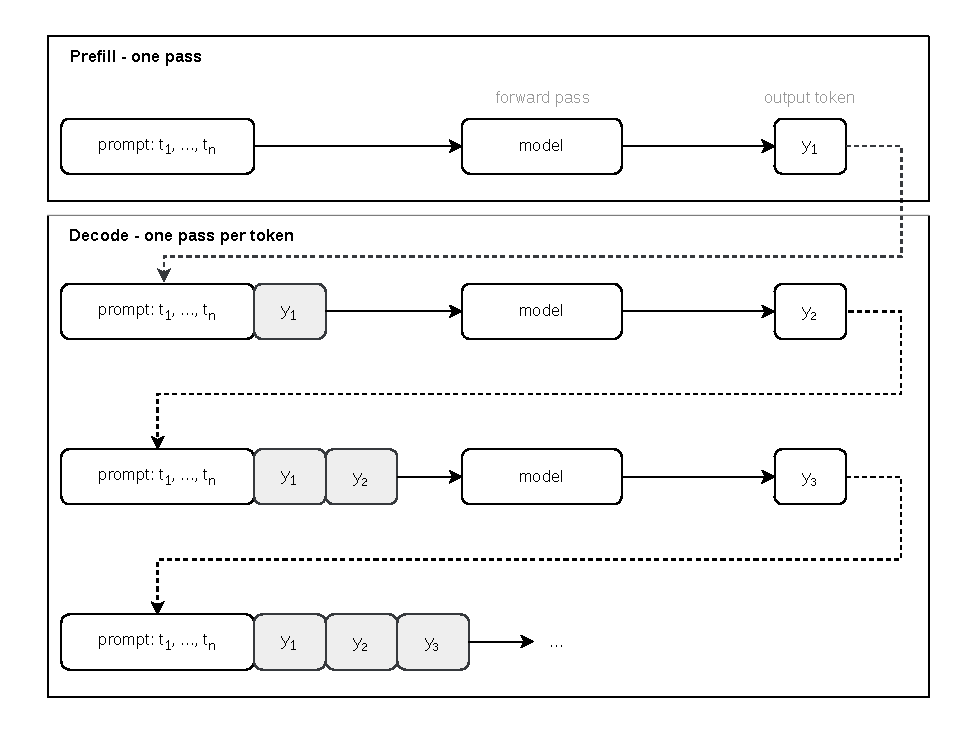
\includegraphics[width=0.9\textwidth]{images/prefill_decode.pdf}
	\caption[Prefill and decode]{Prefill and decode. Prefill processes the whole prompt in a single forward pass and emits the first token. Decode performs one forward pass per token, each time on the input extended by the token emitted at the previous step.}
	\label{fig:prefill-decode}
\end{figure}

The keys and values computed during prefill and at each decode step are stored in the key-value cache \cite{xuKVCacheOptimization2026}. Each decode step then computes attention only for the new token, using the cached keys and values, instead of recomputing attention for all previous tokens.

The distinction between prefill and decode matters for cost. The vectors produced at the last prompt token are produced by the prefill pass, which is executed in any case before the first output token can be emitted. Obtaining them therefore requires no additional forward pass, and no generated tokens. A method that reads the prefill representation and a method that reads the generated text differ in when they can act: the first can act before decoding begins, the second only after it has finished.

\section{Scale, Emergence, and Adaptation}
\label{sec:scale-emergence}

The mechanism described in Section~\ref{sec:transformer} is the same at every model size. Scale changes the range of tasks the model can be used for, instruction tuning changes the form in which a task is supplied to it, and the interface exposed by the provider changes the form in which the answer is returned.

\subsection{Scale and emergent abilities}
\label{subsec:scale}

Transformer-based language models have been scaled to progressively larger sizes. Once pretrained models reached on the order of a hundred billion parameters, their behavior diverged from that of smaller predecessors. In 2020, Brown et al. reported that GPT-3 could perform a wide range of tasks given only a natural-language prompt and a few examples, with no gradient updates \cite{brownLanguageModelsAre2020}. A separate line of work has identified \emph{emergent abilities}, capabilities such as multi-step reasoning and multi-digit arithmetic that do not improve smoothly with scale but appear only beyond a certain model size \cite{weiEmergentAbilitiesLarge2022, zhaoSurveyLargeLanguage2026}.

\subsection{Foundation models and adaptation by prompt}
\label{subsec:foundation-models}

A Large Language Model (or LLM) is an instance of a foundation model: a model trained on broad data, generally through self-supervision at scale, that can be adapted to a wide range of downstream tasks rather than trained for any one of them \cite{bommasaniOpportunitiesRisksFoundation2022}. Bommasani et al. chose the term \emph{foundation} to name this role: the model is itself incomplete, but it serves as the common basis from which many task-specific models are built through adaptation \cite{bommasaniOpportunitiesRisksFoundation2022}. The breadth of the training data reduces the need to encode task-specific information in the model, so one general model can replace many task-specific ones. The model can be adapted to a particular task by supplying a prompt that states the task in natural language, with no retraining \cite{bommasaniOpportunitiesRisksFoundation2022,brownLanguageModelsAre2020}. The task is therefore part of the input, and it occupies token positions of the sequence described in Section~\ref{sec:transformer} like any other content.

\subsection{Frozen models}
\label{subsec:frozen}

Adaptation by prompt changes no parameter of the model: the weights set during pretraining, and during any later fine-tuning, stay fixed while the model is used \cite{bommasaniOpportunitiesRisksFoundation2022,brownLanguageModelsAre2020}. A model whose parameters receive no gradient update while it is used, whether it is adapted by prompt or simply run as is, is referred to throughout this work as \emph{frozen}.

\subsection{Instruction tuning and the chat format}
\label{subsec:instruction-tuning}

Instruction following is not a direct result of scale: next-token prediction does not align the output with what a user intends, and larger models can be as untruthful or unhelpful as smaller ones \cite{ouyangTrainingLanguageModels2022}. Instruction tuning addresses this: a pretrained model is fine-tuned on demonstrations of desired behavior and then refined with reinforcement learning from human feedback, producing a system that follows natural-language instructions across many tasks \cite{ouyangTrainingLanguageModels2022, zhaoSurveyLargeLanguage2026}.

Instruction tuning also sets a fixed input format. Instruction-tuned models are queried through a chat format that delineates roles, such as a system instruction, a user message, and previous assistant turns \cite{openaiGptoss120bGptoss20bModel2025}. The prompt processed at inference time is the rendering of these roles into a single token sequence, as Section~\ref{sec:terminology} defines in detail.

\subsection{Chain-of-thought prompting}
\label{subsec:chain-of-thought}

Adaptation by prompt also covers how the answer is produced, and not only what task is asked. Wei et al. introduced \emph{chain-of-thought} prompting, in which the prompt contains demonstrations that state a series of intermediate reasoning steps before the answer. The model then generates the same kind of steps before its answer to the query \cite{weiChainofThoughtPromptingElicits2023}. They reported that the technique improves performance on arithmetic, commonsense, and symbolic reasoning tasks, and that prompting a 540B-parameter model with eight such demonstrations reaches state-of-the-art accuracy on the GSM8K benchmark of math word problems \cite{weiChainofThoughtPromptingElicits2023}. The gains appear only in sufficiently large models, which places the technique alongside the emergent abilities of Section~\ref{subsec:scale} \cite{weiChainofThoughtPromptingElicits2023, weiEmergentAbilitiesLarge2022}.

The intermediate steps are produced by ordinary token generation: each step is a span of tokens, emitted one at a time in the decode phase of Section~\ref{subsec:prefill-decode}, and each token is appended to the input before the next is predicted. The technique changes the sequence the answer is computed from: it now contains the model's own intermediate output.

Current model families make this behavior part of the model rather than of the prompt. Some expose it as a mode selected at inference time within one model \cite{yangQwen3TechnicalReport2025, teamGemma4Technical2026}, and some are released to produce chain-of-thought output by default \cite{openaiGptoss120bGptoss20bModel2025}.

\subsection{Structured output and function calling}
\label{sec:structured-output}

A language model emits tokens, so any output with a defined shape has to be produced as text that conforms to that shape. OpenAI introduced function calling as an API feature, later also referred to as tool calling. It makes this a first-class feature of the model interface \cite{FunctionCallingOther2024}. A set of functions is declared with names, descriptions, and argument schemas, and the model returns a structured object that names one of the declared functions and supplies its arguments, instead of free-form text \cite{FunctionCallingOther2024}.

The declarations are part of the prompt: the names, descriptions, and schemas of the available functions are rendered into the token sequence the model processes.

The model does not execute the function it calls. The calling application runs the named function with the supplied arguments, and the result is sent back to the model as a new turn. The model then continues generation using that result, typically to produce a final response that incorporates it \cite{FunctionCallingOther2024}.

\section{Defining the Prompt}
\label{sec:terminology}

Section~\ref{subsec:instruction-tuning} introduces the \emph{prompt} as the rendering of chat-format roles into one token sequence, together with other information such as function call definitions. However, the term prompt is also commonly used to name the request submitted to a model. This work distinguishes between the two senses, since the rest of it does not use them interchangeably.

\subsection{Query, turn, system prompt, and prompt}
\label{subsec:query-prompt}

The terms \emph{query}, \emph{input}, or \emph{request} name the text a user submits to a large language model. The \emph{response} is the sequence of tokens the model generates after a given request. Together, a request and its response form one \emph{turn} of a conversation. The model may also be invoked with a \emph{system prompt}, an instruction that states the model's role and the behavior it must follow, and is placed before the user turns in the rendered sequence \cite{openaiGptoss120bGptoss20bModel2025}. Finally, function calling declarations like the ones described in Section~\ref{sec:structured-output} (also known as \emph{tool definitions}) can be part of the information supplied to the model. Altogether, this information forms a single prompt, the actual content submitted to the model.

\begin{table}[htbp]
\centering
\begin{tabularx}{\textwidth}{@{}>{\raggedright\arraybackslash}p{0.27\textwidth}X@{}}
\toprule
\textbf{Term} & \textbf{What it names} \\
\midrule
\emph{query}, \emph{input}, or \emph{request} & one message a user submits to obtain a response \\[4pt]
\emph{response} & the text the model generates in response to a request \\[4pt]
\emph{turn} & a request together with the response it receives \\[4pt]
\emph{system prompt} & an instruction that states the model's role and the behavior it must follow, supplied by the application rather than by the user, and placed before the user turns in the rendered sequence \cite{openaiGptoss120bGptoss20bModel2025} \\[4pt]
\emph{prompt} & the full token sequence a model reads: the system prompt and every turn of the conversation so far, rendered together, plus any declared functions when function calling is enabled (Section~\ref{sec:structured-output}) \\
\bottomrule
\end{tabularx}
\caption[Terms for a query and its surrounding prompt]{The terms this work uses for a query and for the prompt built around it.}
\label{tab:terminology}
\end{table}


\subsection{A rendered example}
\label{subsec:rendered-example}

The rendering of the prompt is defined by a separate chat template. Figure~\ref{fig:rendered-example} shows how Qwen3-4B-Instruct \cite{yangQwen3TechnicalReport2025} renders this template when the query ``Are you able to research online?'' is submitted to a model, together with a specific system prompt and a tool definition that allows the model to request a web search.

\begin{figure}[htbp]
\centering
\footnotesize
\begin{tabularx}{\textwidth}{X}
\toprule
\texttt{<|im\_start|>system} \\
\texttt{You are a helpful assistant. You can search online if you need current information.} \\
\texttt{\# Tools} \\
\texttt{You may call one or more functions to assist with the user query. You are} \\
\texttt{provided with function signatures within <tools></tools> XML tags:} \\
\texttt{<tools>} \\
\texttt{\{"type": "function", "function": \{"name": "web\_search", "description":} \\
\texttt{"Search the web for a query and return matching results.", "parameters":} \\
\texttt{\{"type": "object", "properties": \{"query": \{"type": "string", "description":} \\
\texttt{"The search query."\}\}, "required": ["query"]\}\}\}} \\
\texttt{</tools>} \\
\texttt{For each function call, return a json object with function name and arguments} \\
\texttt{within <tool\_call></tool\_call> XML tags:} \\
\texttt{<tool\_call>} \\
\texttt{\{"name": <function-name>, "arguments": <args-json-object>\}} \\
\texttt{</tool\_call><|im\_end|>} \\
\texttt{<|im\_start|>user} \\
\texttt{Are you able to research online?<|im\_end|>} \\
\texttt{<|im\_start|>assistant} \\
\bottomrule
\end{tabularx}
\caption[Full prompt rendered with the Qwen3-4B-Instruct chat template]{A full prompt rendered using the Qwen3-4B-Instruct chat template.}
\label{fig:rendered-example}
\end{figure}

The rendered sequence ends right after the \texttt{assistant} role tag, with no content after it. This is the point where generation starts, and it corresponds to the last prompt token discussed in Section~\ref{subsec:last-token}.

Each call to the model is stateless: nothing from a prior call is retained, so any content the model must read again is included in any subsequent prompt.

Suppose the model answers the request of Figure~\ref{fig:rendered-example} with ``Yes, I can search the web if the question needs current information.'', completing the first turn, and the user then asks ``What is the weather in London today?''. Figure~\ref{fig:rendered-example-2} shows the prompt for this second call. The system prompt and the tool declaration are unchanged from Figure~\ref{fig:rendered-example} and are rendered again in full. What is added is the first turn and the new request.

\begin{figure}[htbp]
\centering
\scriptsize
\begin{tabularx}{\textwidth}{X}
\toprule
\texttt{<|im\_start|>system} \\
\texttt{You are a helpful assistant. You can search online if you need current information.} \\
\texttt{\# Tools} \\
\texttt{You may call one or more functions to assist with the user query. You are} \\
\texttt{provided with function signatures within <tools></tools> XML tags:} \\
\texttt{<tools>} \\
\texttt{\{"type": "function", "function": \{"name": "web\_search", "description":} \\
\texttt{"Search the web for a query and return matching results.", "parameters":} \\
\texttt{\{"type": "object", "properties": \{"query": \{"type": "string", "description":} \\
\texttt{"The search query."\}\}, "required": ["query"]\}\}\}} \\
\texttt{</tools>} \\
\texttt{For each function call, return a json object with function name and arguments} \\
\texttt{within <tool\_call></tool\_call> XML tags:} \\
\texttt{<tool\_call>} \\
\texttt{\{"name": <function-name>, "arguments": <args-json-object>\}} \\
\texttt{</tool\_call><|im\_end|>} \\
\texttt{<|im\_start|>user} \\
\texttt{Are you able to research online?<|im\_end|>} \\
\texttt{<|im\_start|>assistant} \\
\texttt{Yes, I can search the web if the question needs current information.<|im\_end|>} \\
\texttt{<|im\_start|>user} \\
\texttt{What is the weather in London today?<|im\_end|>} \\
\texttt{<|im\_start|>assistant} \\
\bottomrule
\end{tabularx}
\caption[Next-call prompt rendered with Qwen3-4B-Instruct chat template]{The prompt for the next call in the same conversation, rendered using the Qwen3-4B-Instruct chat template.}
\label{fig:rendered-example-2}
\end{figure}

The whole conversation, not only the new request, is resent at every call. An LLM can therefore handle conversations despite being completely stateless.

\section{Constraints and Limitations}
\label{sec:properties}

The properties of large language models stated in this section constrain what any system built around them can guarantee. They are consequences of how the model is trained and queried, and they are stated here because the rest of this work depends on them.

\paragraph{Stochasticity.} Each output of a large language model is sampled from a distribution over tokens rather than read from a deterministic policy, according to the decoding strategy of Section~\ref{subsec:decoding}. Two runs on the same input can therefore return different outputs. Song et al. showed that this variability is large enough to affect benchmark conclusions \cite{songGoodBadGreedy2024}. The same model can score differently under greedy decoding and under sampling, and the gap is observed across model families and benchmarks \cite{songGoodBadGreedy2024}. The same analysis reported that the ranking of two models can change with the decoding configuration, so a comparison between models holds only for a fixed configuration \cite{songGoodBadGreedy2024}. The effect compounds in a system that chains many model calls: the variance of each call carries into the next, so two runs on the same task can reach different outcomes through different paths.

\paragraph{Context dependence.} Model behavior depends on the prompt and on whatever else occupies the context window, not on encoded rules or a stable policy. The position of the relevant content in the context is one factor. By keeping the input fixed and moving the document that contains the answer, Liu et al. reported that performance is highest when that document is at the beginning or at the end of the input context and degrades when the model must use it in the middle \cite{liuLostMiddleHow2023a}. The performance of GPT-3.5-Turbo on multi-document question answering drops by more than 20\% under this change, and when the answer document is placed in the middle of the context (the worst position), performance is lower than that of the same model with no documents supplied at all \cite{liuLostMiddleHow2023a}. Models with an extended context window are not better at using their input context than their non-extended counterparts \cite{liuLostMiddleHow2023a}. The effective policy is implicit in the model and in the context assembled around it, and it shifts whenever any part of that context changes.

\paragraph{Instruction following.} Instructions in the prompt state what the model is asked to do, and those instructions are not always followed. Zhou et al. measured this on instructions whose satisfaction a program can check, such as a word limit or a required keyword, using 25 instruction types over about 500 prompts \cite{zhouInstructionFollowingEvaluationLarge2023}. GPT-4 satisfies every verifiable instruction of a prompt in 76.89\% of the prompts, and PaLM 2 S in 43.07\% \cite{zhouInstructionFollowingEvaluationLarge2023}. The instructions measured this way are the ones that are easiest to state without ambiguity. The same work notes that language is subjective, and that the standard for an instruction such as writing with a funny tone is unclear \cite{zhouInstructionFollowingEvaluationLarge2023}.

\paragraph{Hallucination.} Large language models generate content that conflicts with the source available to them, called intrinsic hallucination, or that cannot be verified against that source, called extrinsic hallucination \cite{zhaoSurveyLargeLanguage2026, huangSurveyHallucinationLarge2025}. Hallucination occurs widely in existing models, including the most capable ones \cite{zhaoSurveyLargeLanguage2026}, and the false content is produced with high confidence \cite{wangSurveyLargeLanguage2024}.

\section{Hidden States as an Object of Study}
\label{sec:hidden-states}

The emitted tokens are the only part of a forward pass that the application calling the model observes, but the pass also produces one vector per layer and per position. These vectors are the object of study of this section.

\subsection{What a hidden state is}
\label{subsec:hidden-states}

The \emph{hidden state} of a model at layer $\ell$ and position $i$ is the vector produced at that position by block $\ell$. This vector is the value carried into block $\ell+1$. It is written here as
\begin{equation}
    h^{(\ell)}_i ,
    \qquad \ell = 1, \dots, L ,
    \qquad i = 1, \dots, n ,
\end{equation}
where $L$ is the number of blocks and $n$ is the number of tokens in the input. Each $h^{(\ell)}_i$ is a vector of dimension $d_{\mathrm{model}}$. One forward pass therefore produces $L \times n$ such vectors.

\begin{figure}[ht]
	\centering
	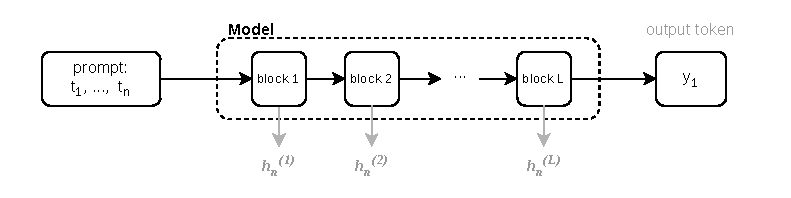
\includegraphics[width=0.9\textwidth]{images/hidden-states-ex.pdf}
	\caption[Hidden states across blocks]{The hidden states written at the last prompt token, $h^{(1)}_n, \dots, h^{(L)}_n$.}
	\label{fig:hidden-states}
\end{figure}

The set of these vectors is the representation that the model forms of the input while it processes it. At a fixed position, the vectors at increasing $\ell$ are successive states of the same representation, since each block reads the value produced by the previous one and writes an updated value into it. The prediction is refined block by block as a result \cite{gevaTransformerFeedForwardLayers2021, belroseElicitingLatentPredictions2025}. The content of these states depends on the layer. Ethayarajh measured how much the representation of a word varies with the context it appears in, on ELMo, BERT and GPT-2, and reported that the higher the layer, the more context-specific the representation is \cite{ethayarajhHowContextualAre2019}. After correcting for a property of these representations called anisotropy (Section~\ref{subsec:anisotropy}), Ethayarajh computed the first principal component of a word's representations across its contexts, a single fixed vector, and measured how much of the variation in those representations it explained. In every layer of the three models, on average, that vector explained less than 5\% of the variance in the word's representations across contexts. A word therefore has no small set of fixed senses that the model picks from: its representation differs in almost every context \cite{ethayarajhHowContextualAre2019}.

The last hidden state, $h^{(L)}_n$, is the vector to which the unembedding of Section~\ref{subsec:unembedding} is applied.

\subsection{Probing as a method}
\label{subsec:probing-method}

Reading a property off the hidden states is defined as \emph{probing}. A \emph{probe} is a classifier trained to predict a property of interest from the representations of a frozen model, and trained independently of the model itself \cite{alainUnderstandingIntermediateLayers2018a}. The representations are the input of the classifier and the property is its label, so the accuracy of the probe measures the degree to which the property is recoverable from the representation it is fitted on \cite{alainUnderstandingIntermediateLayers2018a}. Probing classifiers have become one of the main methods for analyzing neural models of natural language processing, and their methodological limitations have been reviewed critically \cite{belinkovProbingClassifiersPromises2021a}.

A probing result is limited both by what a high accuracy can establish and by the probe itself. A high accuracy establishes that a property is decodable from a representation. It does not establish that the model uses the property to produce its output \cite{belinkovProbingClassifiersPromises2021a}. Orgad et al. found that a model can encode the correct answer and consistently generate an incorrect one; this is the empirical form of the same distinction, since the property is present in the representation while the output does not reflect it \cite{orgadLLMsKnowMore2025}. The probe itself is a further limitation. A classifier with enough capacity can memorize the labels of the training data, achieving high accuracy even if the representation carries little of the property. In that case, the accuracy reflects the probe's own capacity, not the representation. A control baseline, a probe trained on the same task with the labels replaced by a version that carries no real signal, such as randomly shuffled labels, is therefore required: if the control also reaches high accuracy, the fitted probe's accuracy reflects its capacity to memorize rather than any property of the representation \cite{belinkovProbingClassifiersPromises2021a}.

A probe is commonly restricted to a linear classifier, because this matches how a property is expected to be encoded: not by one coordinate of the representation, but by its projection onto one fixed direction in the representation space, which is exactly what a linear classifier reads. Marks and Tegmark found that the truth or falsehood of a factual statement is linearly represented at sufficient model scale, and that shifting a representation along the identified direction changes the output of the model accordingly \cite{marksGeometryTruthEmergent2024}. Wu et al. reported the same form for the tool a model is about to call, which is carried by one direction per pair of tools and can be used to switch the selected tool \cite{wuToolCallingLinearly2026}. A linear probe's accuracy therefore measures whether the property is available as such a projection. Restricting the probe to a linear classifier also bounds its capacity, so the same kind of control baseline is needed to separate what the representation carries from what the probe learns from the labels \cite{belinkovProbingClassifiersPromises2021a}. With this control baseline in place, a high probe accuracy shows only that the property is decodable from the representation. It does not show that the model relies on this property when it produces its output.

\subsection{Anisotropy}
\label{subsec:anisotropy}

All representations of a given layer have high cosine similarity to each other, regardless of the word each one represents. This tendency is called \emph{anisotropy}: representations concentrate in a narrow region of the space instead of spreading in every direction \cite{ethayarajhHowContextualAre2019}. Anisotropy inflates the similarity between any two representations. For this reason, the measurement described in Section~\ref{subsec:hidden-states} is corrected before it measures how word-specific a representation is: Ethayarajh subtracted a baseline, the average similarity between representations of randomly sampled words at the same layer \cite{ethayarajhHowContextualAre2019}.

LatentGate, a hidden-state router discussed in Section~\ref{subsec:latentgate}, identifies anisotropy as a mechanism behind the failure of its embedding baselines, and corrects it with PCA-whitening before training its probe \cite{ratnakarLatentGateLowLatencySemantic2026}. Whether this correction helps a probe is debated. Forooghi et al. found the opposite pattern for classification tasks in large language models: whitening consistently degraded classification accuracy, across 8 models and 7 datasets \cite{forooghiWhiteningNotRecommended2024}.

\subsection{Choosing a Position to Probe}
\label{subsec:last-token}

Because attention in a decoder-only model is masked, the hidden state at position $i$ is computed from the first $i$ tokens only. Probing therefore requires a choice of which position to read the hidden state from, since different positions carry different information.

The last token of the prompt (Section~\ref{sec:terminology}) is the only position whose representation is computed with access to the entire prompt, and it is also the position from which the first generated token is predicted. Any information the model uses to select the first generated token has to be present in the hidden state at the last prompt token. As a result, the hidden state at the last prompt token carries the information behind the decision the model is about to state, before it produces any output token. A hidden state read at an earlier position instead carries only a partial representation of the prompt.

Healy et al. compared ten ways of extracting hidden states from a query, including reading the last token alone, and various pooling of all the token hidden states, and reported that detection accuracy varies with the choice, from 73.9\% to 74.6\% on their tool-call hallucination task \cite{healyInternalRepresentationsIndicators2026}. The probe position therefore influences the accuracy of the probe and should be evaluated for each task.

\subsection{Layer depth as an axis}
\label{subsec:layer-depth}

The layer index $\ell$ marks the depth at which a hidden state is read. Depth is an axis along which the content of the representation changes, and different layers can carry different amounts of information about a given property. Alain and Bengio introduced the practice of training an independent linear classifier on each layer of a frozen network. They used it to measure how suitable each layer's features are for a classification task, and reported on image classifiers that linear separability increases monotonically with depth \cite{alainUnderstandingIntermediateLayers2018a}. For language models the reported pattern is not monotonic: Azaria and Mitchell found that the accuracy of a truthfulness classifier depends on which layer supplies the activations, rather than being highest at the last one \cite{azariaInternalStateLLM2023}. Geva et al. and Belrose et al. gave a consistent account of why the layer index is informative: the representation is refined progressively, so its content differs between lower and upper blocks \cite{gevaTransformerFeedForwardLayers2021, belroseElicitingLatentPredictions2025}.

The number of blocks is not comparable across models: two models with similar parameter counts can differ in depth. Comparing layers across models therefore requires the depth index to be normalized by the total number of blocks rather than used directly.

\subsection{What the evidence supports}
\label{subsec:readability}

The claim that the intermediate values are informative rests on empirical results, not on an assumption. Belrose et al. showed that a probe trained on a single Transformer block decodes that block's hidden state into a usable prediction, and that the resulting trajectory of latent predictions can be used to detect malicious inputs with high accuracy \cite{belroseElicitingLatentPredictions2025}. Azaria and Mitchell trained a classifier on the hidden layer activations of a model as it reads or generates a statement, and obtained between 71\% and 83\% accuracy in labeling statements as true or false, depending on the base model \cite{azariaInternalStateLLM2023}. Orgad et al. reported that information of this kind is concentrated in specific tokens rather than spread uniformly across the sequence, and that exploiting this concentration improves error detection \cite{orgadLLMsKnowMore2025}. Wu et al. reported that which tool a model is going to call is encoded as a direction in activation space, and that this direction is readable before the call is generated \cite{wuToolCallingLinearly2026}. These results span distinct properties, factual truth, malicious intent, and tool selection, so decodability from the hidden state is not confined to one narrow signal.

These results hold under limits. Section~\ref{subsec:anisotropy} described a tendency of hidden states to already point in similar directions, corrected for before measuring how word-specific a representation is. Anisotropy means that two hidden states can have high cosine similarity for reasons unrelated to the property of interest, which constrains any method that compares hidden states directly. The constraint applies to methods that decide by similarity between representations, such as nearest-neighbour assignment or matching against a class centroid. It does not apply to a probe of the kind defined in Section~\ref{subsec:probing-method}, which is fitted on labelled examples and reads a direction in the space rather than a distance between two points. Orgad et al. further found that detectors trained on internal states fail to generalize across datasets \cite{orgadLLMsKnowMore2025}.

The results support a limited statement: a property is sometimes recoverable from the internal state of a model that does not state it, and whether it is recoverable in a given setting has to be measured rather than assumed.


\chapter{LLM-based Agents}
\label{chap:agents}

In artificial intelligence, an agent is a system that operates autonomously, perceives its environment, persists over time, adapts to change, and creates and pursues goals \cite[Chap.~2]{russellArtificialIntelligenceModern2022}. The associated operational model describes the system as reading its environment through sensors and acting on it through actuators. The agent itself is defined by the mapping between these two interfaces \cite[Chap.~2]{russellArtificialIntelligenceModern2022}. This chapter reviews that classical notion and contrasts it with the LLM-based agent. It then describes how single agents are composed into multi-agent systems and coordinated by the routing pattern this work studies.

\section{The Classical Notion of an Autonomous Agent}
\label{sec:classical-agent}

\subsection{Rationality and the perceive-decide-act loop}
\label{subsec:rationality}

A rational agent selects the action that achieves the best outcome or, when outcomes are uncertain, the best expected outcome \cite[Chap.~2]{russellArtificialIntelligenceModern2022}. Such systems are described by the following elements \cite[Chap.~2]{russellArtificialIntelligenceModern2022}:

\begin{itemize}
	\item The \emph{performance measure}, an external criterion that defines the notion of best by scoring the consequences of the agent's behavior on the environment, specified in terms of states of the world.
	\item The \emph{agent function}, the abstract mapping from percepts to actions, where a percept is the perceptual input available to the agent at a given instant.
	\item The \emph{agent program}, the concrete implementation that produces those actions on a physical or computational machine.
\end{itemize}

Figure~\ref{fig:rational-agent} summarizes these elements and their relations.

\begin{figure}[ht]
	\centering
	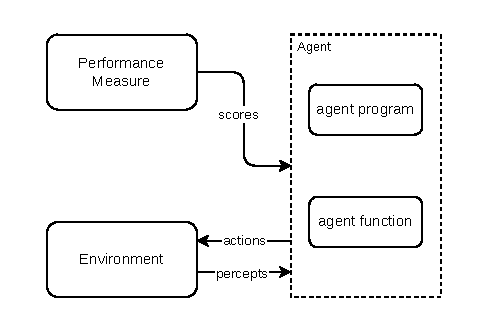
\includegraphics[width=0.6\textwidth]{images/rational_agent.pdf}
	\caption[An autonomous agent]{An autonomous agent}
	\label{fig:rational-agent}
\end{figure}

Independently of its internal design, an agent program implements the same three-step pattern. The system observes the environment, decides what to do, and acts. The action may change the environment; the resulting state is observed, and the cycle repeats. This is the perceive-decide-act loop \cite[Chap.~2]{russellArtificialIntelligenceModern2022}. Rationality is realized in the decide step, where the agent selects the action that, given the available percepts, is expected to maximize the performance measure.

The loop above treats perception as the agent receiving whatever percept the environment provides. Some actions are instead chosen to affect what the agent perceives next rather than to change the state of the environment. This is called information gathering, an action planned for the purpose of reducing the agent's uncertainty about the environment \cite[Chap.~2]{russellArtificialIntelligenceModern2022}. Bajcsy characterizes perception as active, by analogy to biological vision, where the sensing apparatus is continuously adjusted rather than left to record whatever reaches it \cite{bajcsyActivePerception1988}. Under this view, the agent also controls its own data acquisition, through strategies that depend on the goal of the task and on the current state of the interpretation. The choice of what to measure, where to look, and when enough has been observed is formulated as a search that minimizes a loss while seeking the most informative data \cite{bajcsyActivePerception1988}. The control is guided by prior knowledge, in a knowledge-driven regime: the agent's models and expectations direct what it looks for. This has a cost: acquisition can be steered toward what is expected, so unanticipated objects can go undetected \cite{bajcsyActivePerception1988}. The perceive and decide steps are therefore mutually dependent, because the percepts that the decide step acts on are partly the result of earlier choices about what to acquire.

\subsection{Approaches to building agents}
\label{subsec:building-approaches}

Russell and Norvig identify four kinds of agent program that realize the decide step: simple reflex, model-based reflex, goal-based, and utility-based agents \cite[Chap.~2]{russellArtificialIntelligenceModern2022}. Each extends the previous one to remove one of its limitations, and any of the four can in addition be made a learning agent, whose components are acquired from experience instead of being fixed by the designer \cite[Chap.~2]{russellArtificialIntelligenceModern2022}. None of them removes the requirement that the designer specify the task in advance. What changes across the four is the form that the specification takes. Each kind chooses its action from the agent's \emph{current state}, the description of the relevant aspects of the environment at the present instant. A simple reflex agent takes the current state directly from the current percept, but the others reconstruct it from the percept history using a model of the environment \cite[Chap.~2]{russellArtificialIntelligenceModern2022}. Table~\ref{tab:agent-designs} summarizes how each design selects an action, what the designer has to supply, and the limitation that remains.

\begin{itemize}
	\item The \emph{simple reflex agent} realizes the decide step as condition-action rules on the current percept, which works only when the environment is fully observable \cite[Chap.~2]{russellArtificialIntelligenceModern2022}.
	\item The \emph{model-based reflex agent} maintains an internal state to track what the current percept does not reveal, which requires a transition model of how the environment evolves and a sensor model of how its state is reflected in the percepts \cite[Chap.~2]{russellArtificialIntelligenceModern2022}.
	\item The \emph{goal-based agent} adds a description of the desirable situations and selects actions predicted to lead to them, which requires consideration of the future. When a single action does not suffice, this also requires search and planning over a domain model that the designer writes in advance \cite[Chap.~2]{russellArtificialIntelligenceModern2022}. Planning of this kind is computationally costly \cite[Chap.~2]{russellArtificialIntelligenceModern2022}. Hierarchical task network planning reduces the cost by using a plan library of known methods that implement high-level actions, so the planner searches only the sequences allowed by the library instead of the full space of primitive actions \cite[Chap.~11]{russellArtificialIntelligenceModern2022}.
	\item The \emph{utility-based agent} replaces the goal's plain test of whether a state is reached or not with a utility function over states of the world, the internal counterpart of the performance measure, and selects the action that maximizes expected utility \cite[Chap.~2]{russellArtificialIntelligenceModern2022}.
\end{itemize}

Learning is not a separate design for the decide step but a method for improving the components of any of the previous designs \cite[Chap.~2]{russellArtificialIntelligenceModern2022}. A learning agent is decomposed into three components \cite[Chap.~2]{russellArtificialIntelligenceModern2022}. The performance element is the action-selecting program described so far. A learning element modifies it using feedback from a critic, which measures performance against a fixed standard. A problem generator proposes exploratory actions. In its reinforcement-learning instance, the feedback is a reward signal and the agent refines a mapping from percepts to actions through interaction with the environment \cite[Chap.~23]{russellArtificialIntelligenceModern2022}. The cost moves from authoring rules, models, or plans to providing an environment in which to train, a reward function that captures the intended objective, and enough interaction to converge. Dulac-Arnold et al. survey nine challenges that separate laboratory reinforcement learning from production use, including learning from limited samples on the actual system, partial observability and non-stationarity, satisfying safety constraints during training and operation, and specifying a well-posed and aligned reward \cite{dulac-arnoldChallengesRealWorldReinforcement2019}. Each of these typically requires application-specific engineering, and the resulting policy remains tied to the task and to the conditions under which it was trained \cite{dulac-arnoldChallengesRealWorldReinforcement2019}.

\begin{table}[ht]
	\centering
	\small
	\renewcommand{\arraystretch}{1.15}
	\newcolumntype{R}[1]{>{\raggedright\arraybackslash\hsize=#1\hsize}X}
	\begin{tabularx}{\textwidth}{@{}>{\raggedright\arraybackslash}p{2.75cm}R{1.10}R{0.90}R{1.00}@{}}
		\toprule
		Agent type & Action selection & Designer must supply & Principal limitation \\
		\midrule
		Simple reflex & Condition-action rules on the current percept & The rules & Requires a fully observable environment \\
		\addlinespace
		Model-based reflex & Rules over an internal state & Rules, a transition model, a sensor model & No goals and no model of the future \\
		\addlinespace
		Goal-based & Search and planning toward goal states, or refinement from a plan library & A domain model and goals, or a plan library & Planning is costly; competence is bounded by what is authored \\
		\addlinespace
		Utility-based & Maximization of expected utility & A utility function, in addition to a model & The utility function is hard to specify \\
		\addlinespace
		Learning & Any of the above, refined from feedback & A training environment, a reward signal, interaction & The policy is tied to the task and its training conditions \\
		\bottomrule
	\end{tabularx}
	\caption[Comparison of the agent designs]{Comparison of the agent designs.}
	\label{tab:agent-designs}
\end{table}

The decide step is built for a specific task in each of the four designs, whether their components are fixed by the designer or acquired through learning. What the designer must supply is listed in Table~\ref{tab:agent-designs}: the condition-action rules, the transition and sensor models, the domain model and plan library, the utility function, or the training environment and reward signal. Each of these has to be stated in a formal and executable form, over a set of actions fixed in advance, before the agent can act at all.

This requirement is the principal cost of building an agent with these designs. The intended behavior is normally known in informal terms, and the work consists in translating it into a specification that the decide step can execute. This translation demands expertise in the design and in the application domain. It is also incomplete in practice: cases that the specification does not cover produce no useful behavior, and the effort grows with the range of cases that the agent has to handle. The reinforcement-learning case illustrates the same cost in a different form, since the reward signal has to express the intended objective and the training conditions have to reproduce the operating conditions. Each of these requires application-specific engineering \cite{dulac-arnoldChallengesRealWorldReinforcement2019}. Building an agent under these designs is therefore limited less by the loop of Section~\ref{subsec:rationality} than by the difficulty of producing the specification that the decide step needs.

\section{The Language Model as Agent Core}
\label{sec:llm-decision-component}

The approaches described in Section~\ref{sec:classical-agent} share the property summarized in Table~\ref{tab:agent-designs}: the decide step is constructed for each task from rules, models, plans, utility functions, or trained policies, authored or trained by the designer over a closed set of actions and against an explicit specification. In contrast to these approaches, a more recent line of work realizes the decide step with a pretrained large language model, of the kind described in Chapter~\ref{chap:llm}, which serves as the agent's core computation unit \cite{zhaoSurveyLargeLanguage2026}. The resulting systems are referred to here as LLM-based agents. They do not build the decide step for any one task: the task is supplied to the model as input, in natural language, rather than encoded into the decide step in advance. This changes what the designer has to produce, since the desired behavior is stated in the terms in which it is normally known, instead of being translated into rules, models, plans, utility functions, or reward signals. It does not remove the design work, and it raises the separate problem of checking that the desired behavior is the behavior obtained, which Chapter~\ref{chap:evaluating-agents} addresses. Models of this kind have emerged as the decision component of agents \cite{zhaoSurveyLargeLanguage2026}, and the volume of literature on them has grown in recent years \cite{wangSurveyLargeLanguage2024}.

\subsection{The language model as the decide step}
\label{subsec:new-decide-step}

The instruction-tuned model of Section~\ref{sec:scale-emergence} is a stochastic policy that takes a prompt as input, emits a token sequence as output, and generalizes across tasks without being retrained for each one \cite{ouyangTrainingLanguageModels2022}. Because it is a foundation model adaptable across tasks \cite{bommasaniOpportunitiesRisksFoundation2022}, what varies from one agent to another is the prompt that frames the goal, the external operations the agent is allowed to invoke, and the data retrieved into its context, rather than the model itself. The same model can be used inside a coding agent, a customer-support agent, or a research assistant. Constructing a new agent remains an engineering task, but it modifies the inputs supplied to the model rather than the decide step it implements.

The definition of agents given by Anthropic is representative, as it groups workflows and agents together as agentic systems while drawing an architectural distinction between them \cite{BuildingEffectiveAI}:

\begin{quotebox}
``Agent'' can be defined in several ways. Some customers define agents as fully autonomous systems that operate independently over extended periods, using various tools to accomplish complex tasks. Others use the term to describe more prescriptive implementations that follow predefined workflows. At Anthropic, we categorize all these variations as \textbf{agentic systems}, but draw an important architectural distinction between \textbf{workflows} and \textbf{agents}:
\begin{itemize}
	\item Workflows are systems where LLMs and tools are orchestrated through predefined code paths.
	\item Agents, on the other hand, are systems where LLMs dynamically direct their own processes and tool usage, maintaining control over how they accomplish tasks.
\end{itemize}
\end{quotebox}

This distinction is consistent with the one adopted in Section~\ref{sec:classical-agent}, where an agent is distinguished by controlling how it pursues its goal.

\subsection{Tools and perception}
\label{subsec:llm-tools-perception}

Realizing the decide step with a large language model also governs the perceive step. Within the context window, all content is treated uniformly as input. A user instruction, a retrieved document, the output of a previous step, and the result returned by a tool all enter the context as text and affect what the model produces next. Percepts reach the model along two routes:

\begin{itemize}
	\item \textbf{Supplied percepts.} These reach the model without the model taking part in their selection: the user request, an event reported by the environment, or a document placed in the context before the model runs.
	\item \textbf{Obtained percepts.} These are retrieved by the model itself. Through the function-calling interface of Section~\ref{sec:structured-output}, the model can emit a structured call to a tool instead of a final action, and the result of that call returns to the context as the next percept.
\end{itemize}

The exchange of a tool call and its returned result recurs across steps, forming the loop described in Section~\ref{subsec:tool-use-react}. In this loop, not every tool call serves the same purpose. Tool calls may be aimed to:

\begin{itemize}
	\item \textbf{Take actions.} A call issued to change the state of the environment.
	\item \textbf{Gather information.} A call issued only to obtain information the model lacks, without changing the environment, such as reading a file or querying a document store. This is the information gathering of Section~\ref{subsec:rationality}: an action planned to reduce the model's uncertainty about the environment rather than to change it.
\end{itemize}

It is this second kind of call that realizes the active perception of Section~\ref{subsec:rationality}. What is available at a given step is therefore in part the result of the model's own earlier choices. Because of that, the perceive, decide, and act steps are not three phases executed once per iteration, but three processes that overlap in time. Issuing a call is a decision. The call is an action when it changes the environment, and an act of perception when it only retrieves information. The result it returns reopens perception, which feeds the next decision in turn. The dependence on prior knowledge described in Section~\ref{subsec:rationality} applies here as well, where expectations assist interpretation but carry the danger of finding what is expected and not detecting what is not \cite{bajcsyActivePerception1988}.

\subsection{Limitations}
\label{subsec:llm-agent-fit}

LLM-based agents replace the rules, models, plans, utility functions, or reward signals of the classical designs with natural-language instructions, which are easier to define and maintain, but do not carry the same precision or expressiveness: a rule or a reward signal has fixed, unambiguous semantics, while a natural-language instruction can be interpreted differently by the model, or interpreted inconsistently across invocations.

The properties defined in Section~\ref{sec:properties} are also inherited by LLM-based agents, since every step of the perceive-decide-act loop is the output of a model call. The action taken at a step is non-deterministic. The policy the agent is meant to apply, stated as prompt instructions, may not be followed, or only partially followed. As the content supplied to the agent grows, performance may degrade, depending on its length and on the position of the relevant information in it. An agent can also hallucinate information and state it with confidence.

Operating in a loop compounds these properties. Each step's output feeds into the context of later steps, so a non-deterministic choice, an unfollowed instruction, or a hallucination at one step propagates to the steps that follow it \cite{wangSurveyLargeLanguage2024}.

The classical designs provide two guarantees by construction: a fixed action set and an explicit specification of when each action applies. Neither guarantee is available here. The specification is easier to write, and conformance to it is no longer established by construction. Whether the behavior obtained matches the desired behavior has to be determined by observing the system. This is the subject of Chapter~\ref{chap:evaluating-agents}.

\section{Anatomy of an LLM-based Agent}
\label{sec:agent-anatomy}

An LLM-based agent is built around a small set of recurring components: tool use, memory, and planning. Tool use is the defining component, since it extends the language model from a system that emits text to one that can act on its environment. Together, these components produce the trajectory, the ordered sequence of reasoning steps, tool calls, and intermediate outputs that the agent goes through before it returns a final response. The trajectory is the unit on which later evaluation operates.

\subsection{The ReAct loop}
\label{subsec:tool-use-react}

ReAct, short for reasoning and acting, is a method that connects language models to the classical notion of an autonomous agent, later turned into a first-class abstraction by the function-calling interface of Section~\ref{sec:structured-output} \cite{yaoReActSynergizingReasoning2022, FunctionCallingOther2024}. The method described in the paper consists of a prompting technique that prompts the model to generate reasoning traces and task-specific actions in an interleaved manner. On the two interactive decision-making benchmarks ALFWorld and WebShop, it improved the absolute success rate over imitation and reinforcement learning baselines by 34\% and 10\% respectively, while using only one or two in-context examples \cite{yaoReActSynergizingReasoning2022}. The action space is augmented to
\begin{equation}
    \hat{A} = A \cup L,
\end{equation}
where
\begin{itemize}
    \item $A$ is the set of domain actions;
    \item $L$ is the space of language \cite{yaoReActSynergizingReasoning2022}.
\end{itemize}
$L$ is the language the model produces as output. An action drawn from $L$, called a thought, does not affect the environment and produces no observation: it lets the model induce, track, and update plans, handle exceptions, and compose information by reasoning over the current context, updating that context for the steps that follow \cite{yaoReActSynergizingReasoning2022}. An action drawn from $A$ interfaces with an external source, such as a weather API, and returns information into the context. In the original formulation, a frozen language model is prompted with few-shot examples to emit both thoughts and actions, producing a trajectory of interleaved thought, action, and observation steps, with no runtime component beyond the prompt \cite{yaoReActSynergizingReasoning2022}. Figure~\ref{fig:react-example} shows such a trajectory for a query about the weather in the user's city, where the model first retrieves the city and then queries the weather for it.

\begin{figure}[ht]
	\centering
	\vspace{4mm}
	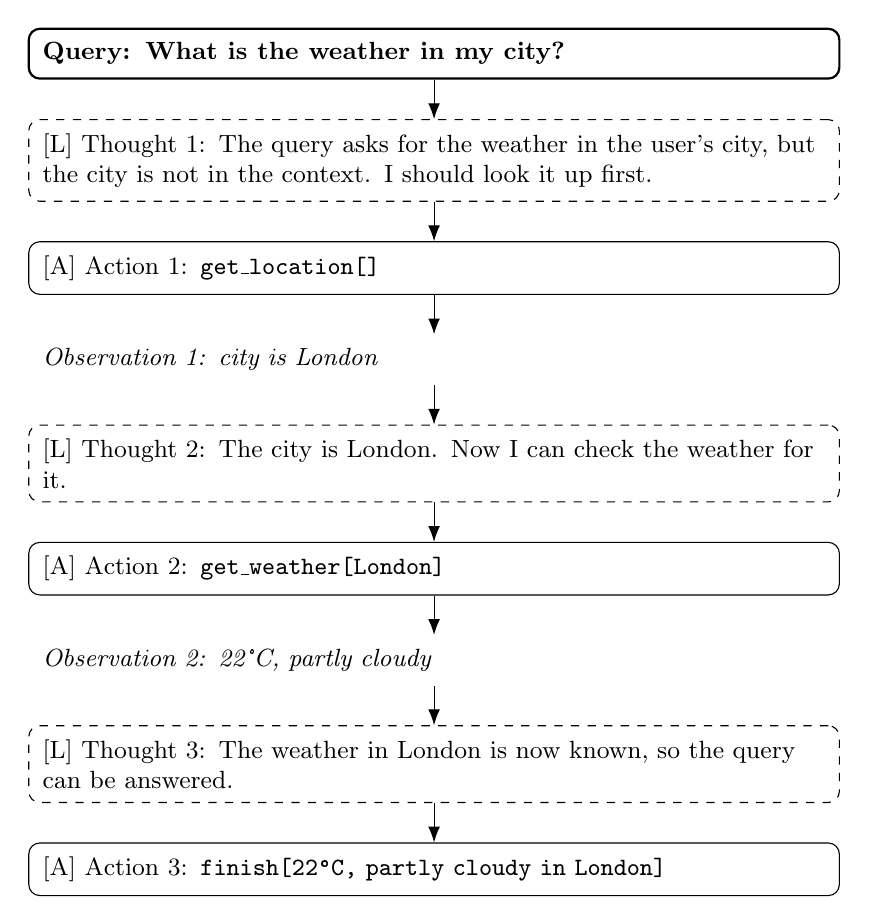
\begin{tikzpicture}[
		node distance=5mm,
		every node/.style={font=\small},
		thought/.style={draw, dashed, rounded corners, align=left, text width=0.82\textwidth, inner sep=5pt},
		action/.style={draw, rounded corners, align=left, text width=0.82\textwidth, inner sep=5pt},
		obs/.style={align=left, text width=0.82\textwidth, inner sep=5pt, font=\small\itshape},
		query/.style={draw, thick, rounded corners, align=left, text width=0.82\textwidth, inner sep=5pt, font=\small\bfseries},
		arr/.style={-{Latex[length=2mm]}}
		]
		\node[query] (q) {Query: What is the weather in my city?};
		\node[thought, below=of q] (t1) {[L] Thought 1: The query asks for the weather in the user's city, but the city is not in the context. I should look it up first.};
		\node[action, below=of t1] (a1) {[A] Action 1: \texttt{get\_location[]}};
		\node[obs, below=of a1] (o1) {Observation 1: city is London};
		\node[thought, below=of o1] (t2) {[L] Thought 2: The city is London. Now I can check the weather for it.};
		\node[action, below=of t2] (a2) {[A] Action 2: \texttt{get\_weather[London]}};
		\node[obs, below=of a2] (o2) {Observation 2: 22\textdegree C, partly cloudy};
		\node[thought, below=of o2] (t3) {[L] Thought 3: The weather in London is now known, so the query can be answered.};
		\node[action, below=of t3] (a3) {[A] Action 3: \texttt{finish[22\textdegree C, partly cloudy in London]}};
		\foreach \x/\y in {q/t1, t1/a1, a1/o1, o1/t2, t2/a2, a2/o2, o2/t3, t3/a3}
			\draw[arr] (\x) -- (\y);
	\end{tikzpicture}
	\caption[An example ReAct trajectory for a weather query]{An example ReAct trajectory for a weather query.}
	\label{fig:react-example}
\end{figure}

In the function-calling interface, each action of Figure~\ref{fig:react-example} becomes a declared function call, such as \texttt{get\_weather(city="London")}, and each observation becomes the value the runtime returns. This interface is architecturally similar to the thought, action, and observation cycle of ReAct, but it separates the concerns of the cycle. The model first declares intent by selecting a function and its arguments, then the runtime executes the call, and the result is injected back into the context as the next input. ReAct couples the generation of the action and its execution within the prompt and the surrounding environment, but function calling assigns execution to the runtime and leaves the model responsible only for declaring the call. Figure~\ref{fig:react-loop} shows the loop as implemented with function calling.

\begin{figure}[ht]
	\centering
	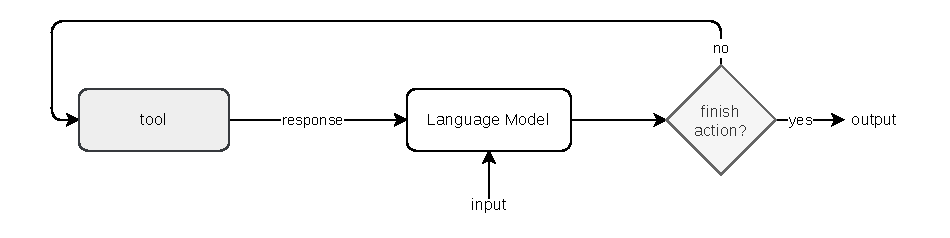
\includegraphics[width=0.92\textwidth]{images/react_loop.pdf}
	\caption[The ReAct loop with tool calling]{The ReAct loop with tool calling}
	\label{fig:react-loop}
\end{figure}

This loop matches the perceive-decide-act cycle of the classical agent of Section~\ref{sec:classical-agent}. The model carries out the decide step; the environment executing a call realizes the act step; the returned response supplies the perceive step. Table~\ref{tab:classical-llm} extends the same correspondence to every component, mapping the elements of the formulation of Russell and Norvig onto their counterparts in an LLM-based agent.
\begin{table}[ht]
	\centering
	\small
	\begin{tabularx}{\textwidth}{@{}XX@{}}
		\toprule
		Classical agent & LLM-based agent \\
		\midrule
		Percept & Content entering the context, including tool results \\
    Actions & Tool calls \\
		Agent function & A forward pass of the language model \\
		Internal state & Context window \\
		Performance measure & External evaluation criterion, applied after the run \\
		\bottomrule
	\end{tabularx}
	\caption[Correspondence between classical agent and LLM-based agents]{Correspondence between classical agent and LLM-based agents.}
	\label{tab:classical-llm}
\end{table}

The performance measure of Section~\ref{subsec:rationality} drives action selection during the run, since the decide step selects the action expected to maximize it \cite[Chap.~2]{russellArtificialIntelligenceModern2022}. An LLM-based agent has no such measure active during the run. It is not built for one task and its objective is defined in the prompt as natural language; therefore, no criterion over states is available to it while it runs. The criterion is applied only after the run, by an evaluation setup that decides both what to evaluate and how to evaluate it \cite{mohammadiEvaluationBenchmarkingLLM2025}. Chapter~\ref{chap:evaluating-agents} describes how such a criterion is defined.

\subsection{Building blocks}
\label{subsec:building-blocks}

So far, the minimal agent has been defined by a language model, a set of tools, and the loop that connects them. On a higher level of abstraction, the loop and the tool definitions allow the agent to be described as a set of components organized around the language model. Zhao et al. and Wang et al. converge on the same three: memory, planning, and an execution component that carries out the plan, called action by Wang et al. \cite{zhaoSurveyLargeLanguage2026, wangSurveyLargeLanguage2024}. Zhao et al. describe the language model as the core computation unit, equipped with these three components and integrated under its control during interactions with the environment \cite{zhaoSurveyLargeLanguage2026}. Wang et al. add a fourth module, profiling, which identifies the role of the agent and influences the memory and planning modules; those two modules, together with profiling, in turn influence the action module \cite{wangSurveyLargeLanguage2024}. The three shared modules are described below. The ReAct loop of Section~\ref{subsec:tool-use-react} sequences their use.

\paragraph{Planning.} The planning component decomposes a complex task into simpler subtasks that are solved individually \cite{wangSurveyLargeLanguage2024}. Wang et al. separated existing designs according to whether the agent receives feedback during the planning process \cite{wangSurveyLargeLanguage2024}:
\begin{itemize}
    \item \emph{Planning without feedback}, where the agent does not receive feedback that can influence its future behavior after taking actions. This covers single-path reasoning, in which the task is decomposed into intermediate steps connected in a pipeline, each leading to a single subsequent step. It also covers multi-path reasoning, in which the steps are organized into a tree and each step may have several subsequent steps, and the delegation of plan generation to a well-developed external planner \cite{wangSurveyLargeLanguage2024}.
    \item \emph{Planning with feedback}, where the agent revises its plans after taking actions on the basis of signals obtained from the environment, from humans, or from a model. This is better suited to complex tasks that need long-horizon planning, where planning without feedback is less effective \cite{wangSurveyLargeLanguage2024}.
\end{itemize}

\paragraph{Memory.} The memory component stores information perceived from the environment and uses the recorded memories to facilitate future actions \cite{wangSurveyLargeLanguage2024}. Wang et al. analyzed it along three perspectives \cite{wangSurveyLargeLanguage2024}:
\begin{itemize}
    \item \emph{Structures}, which distinguish short-term from long-term memory. Short-term memory consists of the information within the context window constrained by the transformer architecture, while long-term memory resembles an external store that the agent can query and retrieve from as needed.
    \item \emph{Formats}, the medium in which the content is stored, including raw natural language, embedding vectors, databases, and structured lists \cite{wangSurveyLargeLanguage2024}.
    \item \emph{Operations}, through which the component interacts with the environment: \textbf{reading}, which extracts relevant information from memory to inform the next action; \textbf{writing}, which stores new information while handling duplication and storage limits; and \textbf{reflection}, which summarizes past records into higher-level insights \cite{wangSurveyLargeLanguage2024}.
\end{itemize}

\paragraph{Action.} The action component translates the agent's decisions into specific outcomes and is located at the most downstream position, where it directly interacts with the environment \cite{wangSurveyLargeLanguage2024}. Two of the perspectives used by Wang et al. bear on the runtime structure \cite{wangSurveyLargeLanguage2024}:
\begin{itemize}
    \item The \emph{action space}, the set of actions available to the agent, divided into external tools and what the model already knows from training. External tools include APIs, databases and knowledge bases, and other models, each of which expands the action space beyond the limitations of the language model on its own \cite{wangSurveyLargeLanguage2024}.
    \item The \emph{action impact}, the consequence of an action, which may change the environment, alter the agent's own internal state such as its memory or plans, or trigger further actions \cite{wangSurveyLargeLanguage2024}.
\end{itemize}

Systems with more than one specialized function add a routing mechanism. It governs the flow of control to different specialized functions, tools, or sub-processes. Through it, the agent evaluates specific criteria and selects from a set of possible subsequent actions instead of following a fixed execution path \cite[Chap.~2]{gulliAgenticDesignPatterns2025}.

Figure~\ref{fig:agent-blocks} shows the complete agent: the language model receives an input and produces a response, drawing on planning and memory and issuing tool calls that act on the environment.

\begin{figure}[ht]
	\centering
	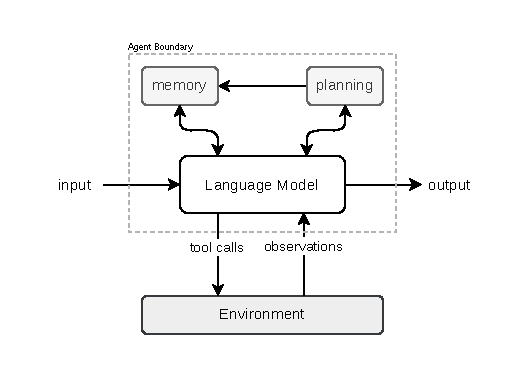
\includegraphics[width=0.75\textwidth]{images/agent_blocks.pdf}
	\caption[The complete LLM-based agent with its building blocks]{The complete LLM-based agent with its building blocks}
	\label{fig:agent-blocks}
\end{figure}

\subsection{Memory and retrieval}
\label{subsec:memory-reml}

The long-term part of the memory component rests on information retrieval. Wang et al. distinguished a unified structure from a hybrid structure \cite{wangSurveyLargeLanguage2024}. A unified structure holds only the short-term memory of Section~\ref{subsec:building-blocks}, directly in the context window. A hybrid structure adds long-term memory: it retrieves relevant records from an external store and inserts them into the prompt, governed by the reading operation and its relevance scoring \cite{wangSurveyLargeLanguage2024}. Retrieval-augmented generation implements this scheme by retrieving relevant information from an external knowledge base, which reduces the generation of factually incorrect content and allows continuous knowledge updates and the integration of domain-specific information \cite{gaoRetrievalAugmentedGenerationLarge2024}. Retrieval introduces failure modes of its own: low precision leads to the selection of misaligned or irrelevant content, and low recall leads to missing crucial information \cite{gaoRetrievalAugmentedGenerationLarge2024}. The model may still produce content not supported by the retrieved context, and it may echo retrieved content without synthesizing it \cite{gaoRetrievalAugmentedGenerationLarge2024}. What enters the context through memory affects every subsequent step, so an error in retrieval propagates through the rest of the loop.

\subsection{Role and configuration}
\label{subsec:agent-identity}

Section~\ref{subsec:new-decide-step} shows that constructing a new agent means changing the prompt, the tools, and the retrieved context, not the model itself. Multiple agents can therefore share the same underlying model and still be told apart, which raises the question of what distinguishes one agent from another, and of whether an agent whose prompt or toolset has changed still counts as the same agent.

The profiling module of Section~\ref{subsec:building-blocks} identifies an agent by its \emph{role}, such as planner, speaker, coordinator, or specialist, written into the prompt to shape the model's behavior \cite{wangSurveyLargeLanguage2024}. Wang et al. use this to populate a system with several distinct agents, for example assigning software-development roles to a collaborating team or generating a population of agents for social simulation \cite{wangSurveyLargeLanguage2024}. In their examples, the role is what tells two agents in the same system apart.

The role and the configuration answer this at two different levels of abstraction, and the two coexist:

\begin{itemize}
	\item At a higher level of abstraction, an agent is defined by the role it occupies, and stays the same agent across a change to its configuration, as long as it keeps the same role.
	\item At a lower level of abstraction, an agent is defined by the prompt, the underlying model, and the toolset made available to it.
\end{itemize}

\section{Multi-Agent Systems}
\label{sec:multi-agent}

A single LLM-based agent, built as in Section~\ref{sec:agent-anatomy}, has limits that grow with the difficulty of the task. Its short-term memory is the information inside the context window, and the transformer architecture bounds it \cite{wangSurveyLargeLanguage2024}. Multi-agent orchestration answers this with a paradigm in which specialized agents assume distinct roles, exchange information through structured protocols, and coordinate their actions to solve problems beyond the reach of any single agent \cite{zhuLLMBasedMultiAgentOrchestration2026a}. Compared with a system that uses a single LLM-based agent, this paradigm specializes LLMs into distinct agents, each with different capabilities, that interact with each other \cite{guoLargeLanguageModel2024}. Section~\ref{sec:coordinator} examines the coordinator-based routing pattern this work studies, in which a coordinator assigns each query to a specialized agent.

Zhu et al. defined the \emph{coordination topology} of a multi-agent system as the directed graph whose vertices are the agents and whose edges are the message-passing or delegation pathways declared at design time \cite{zhuLLMBasedMultiAgentOrchestration2026a}. This graph expresses which agent may direct another, and along which paths messages flow between agents. Their taxonomy has three topologies: centralized, where the graph is a star with a designated supervisor; decentralized, where it is a peer graph with no designated supervisor; and hierarchical, where it is a tree \cite{zhuLLMBasedMultiAgentOrchestration2026a}.

A second axis of the same taxonomy is runtime adaptivity. Here, the active edges are the subset of the topology's edges that carry a message at a given step, distinct from the full edge set declared at design time. A system is static when its vertices, its active edges, and its routing policy are fixed at design time and do not change for the duration of a task, and dynamic-adaptive when that configuration changes at run time, for instance when only the active edge subset changes while the vertices and the permitted edges stay fixed \cite{zhuLLMBasedMultiAgentOrchestration2026a}. The axis is orthogonal to the topology, so any of the three topologies can be static or dynamic-adaptive \cite{zhuLLMBasedMultiAgentOrchestration2026a}.

\subsection{Centralized}
\label{subsec:topology-centralized}

A single supervisor agent owns the workflow: it decomposes the incoming task, assigns subtasks to worker agents, collects their outputs, and decides what happens next \cite{zhuLLMBasedMultiAgentOrchestration2026a}. Every message passes through the supervisor, which therefore keeps a global view of the progress of the task, and the supervisor is typically a language model that reads the current state to select the next worker \cite{zhuLLMBasedMultiAgentOrchestration2026a}. Guo et al. described the same shape as centralized communication, where a central agent coordinates the communication of the system and the other agents interact through this central node \cite{guoLargeLanguageModel2024}. The supervisor is also a single point of failure and a throughput bottleneck, and its context window fills as the number of agents and the length of the conversation grow, which makes the topology suitable for a modest number of agents, roughly three to seven \cite{zhuLLMBasedMultiAgentOrchestration2026a}.

\begin{figure}[ht]
	\centering
	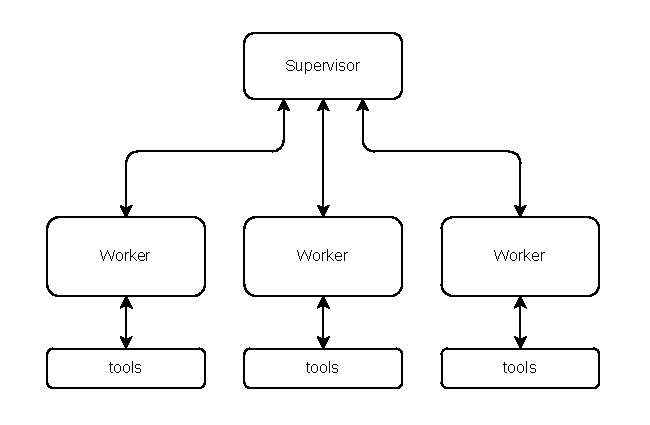
\includegraphics[width=0.72\textwidth]{images/topology_centralized.pdf}
	\caption[Centralized topology]{Centralized topology}
	\label{fig:topology-centralized}
\end{figure}

\subsection{Decentralized}
\label{subsec:topology-decentralized}

No central coordinator exists. The agents communicate directly, and each one decides on its own when to act, whom to consult, and how to contribute. Task allocation emerges from negotiation and self-selection, with each agent holding local state and taking its own routing decisions \cite{zhuLLMBasedMultiAgentOrchestration2026a}. Guo et al. described the same shape as decentralized communication, which operates on a peer-to-peer network where agents communicate directly with each other \cite{guoLargeLanguageModel2024}. They called the corresponding interaction style the debate paradigm, where agents present and defend their own viewpoints or solutions and criticize those of the others to reach a consensus or a more refined solution \cite{guoLargeLanguageModel2024}. The topology removes the single point of failure and lets solutions emerge from unconstrained interaction, but coherent global behavior is hard to guarantee and distributed execution traces make later debugging laborious \cite{zhuLLMBasedMultiAgentOrchestration2026a}. The absence of a single control point also places this topology outside the scope of the routing pattern this work studies, since there is no vertex at which a coordination decision of the kind defined in Section~\ref{sec:coordinator} could be located.

\begin{figure}[ht]
	\centering
	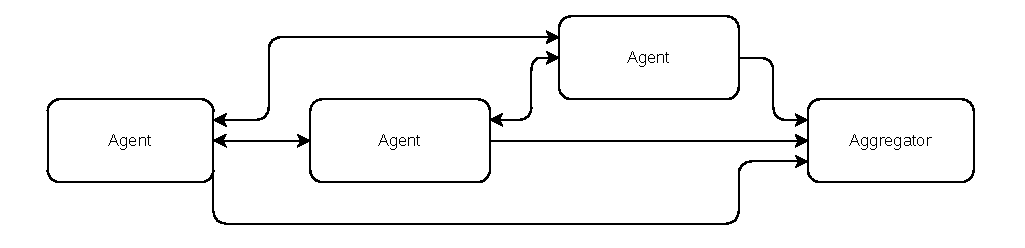
\includegraphics[width=0.88\textwidth]{images/topology_decentralized.pdf}
	\caption[Decentralized topology]{Decentralized topology}
	\label{fig:topology-decentralized}
\end{figure}

\subsection{Hierarchical}
\label{subsec:topology-hierarchical}

The agents are organized in a tree. Manager agents assign subtasks to the level below, and results return to the level above; this is assignment as defined in Section~\ref{sec:coordinator}, since a manager continues the work once its subordinate reports back. Each manager covers one domain or subtask scope and may decompose its assignment further, so top-level managers assign subtasks to mid-level managers and these assign subtasks to leaf-level workers \cite{zhuLLMBasedMultiAgentOrchestration2026a}. An agent that is a worker for its parent is therefore a manager for its own children, and the decision taken once by the supervisor of Figure~\ref{fig:topology-centralized} is repeated at every internal node. Communication scales linearly within the tree rather than quadratically across the full set of agents. This suits large decomposable tasks and systems that must grow beyond ten to fifteen agents, at the cost of the latency of multi-level message passing \cite{zhuLLMBasedMultiAgentOrchestration2026a}. Intermediate managers also become bottlenecks when the tree is not balanced \cite{zhuLLMBasedMultiAgentOrchestration2026a}. Guo et al. described the same shape as layered communication, where agents at each level have distinct roles and interact within their layer or with adjacent layers \cite{guoLargeLanguageModel2024}. Magentic-One extends the pattern with a lead orchestrator that plans, tracks progress, and replans to recover from errors, directing specialized agents for web browsing, file navigation, and code execution \cite{zhuLLMBasedMultiAgentOrchestration2026a}.

\begin{figure}[ht]
	\centering
	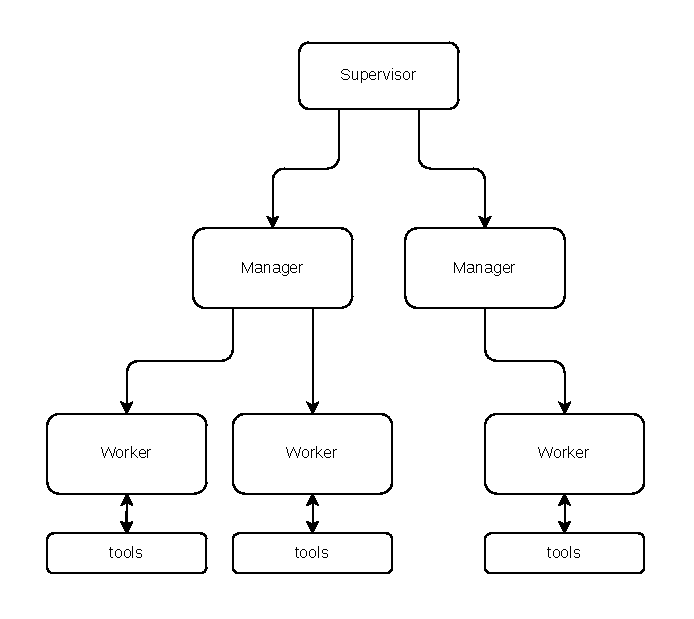
\includegraphics[width=0.7\textwidth]{images/topology_hierarchical.pdf}
	\caption[Hierarchical topology]{Hierarchical topology}
	\label{fig:topology-hierarchical}
\end{figure}



\subsection{Orchestration frameworks}
\label{subsec:topology-frameworks}

These topologies are not merely descriptive categories: they are the constructs that current frameworks expose. Zhu et al. observed that, without a dedicated orchestration layer, agents show three canonical failure modes:
\begin{itemize}
	\item task duplication, where several agents solve the same subtask independently;
	\item contradictory outputs, where agents produce inconsistent artifacts from shared premises;
	\item convergence failure, where the system cycles indefinitely without reaching a terminal state \cite{zhuLLMBasedMultiAgentOrchestration2026a}.
\end{itemize}
The frequency and the severity of these failures increase with the number of agents and the complexity of the task, which is why Zhu et al. treated orchestration as a first-class engineering concern and not as an implementation afterthought \cite{zhuLLMBasedMultiAgentOrchestration2026a}. Every major framework exposes configuration options for it, in the form of speaker-selection policies, delegation flags, conditional edges, and manager swaps. Most frameworks are therefore not restricted to a single cell of the taxonomy and instead cover a small contiguous region of it, with one primary cell obtained from the documented defaults and adjacent cells reachable through configuration \cite{zhuLLMBasedMultiAgentOrchestration2026a}.

\section{The Coordinator Pattern}
\label{sec:coordinator}

Most of the topologies of Section~\ref{sec:multi-agent} require a decision on which agent receives a given unit of work, and the literature names the component that takes it differently depending on the topology: supervisor in a centralized topology, manager at any level of a hierarchical topology \cite{zhuLLMBasedMultiAgentOrchestration2026a}. Both perform the same function, so this work fixes one term for it regardless of topology. Table~\ref{tab:coordinator-terms} defines the terminology used from this point on, \emph{coordinator} for the component that takes the decision, \emph{routing} for the decision itself, and \emph{sub-agent} for each specialized agent it can select, together with the synonyms each term replaces. Those synonyms belong to the topology-specific vocabulary of Section~\ref{sec:multi-agent} and to the source it is drawn from \cite{zhuLLMBasedMultiAgentOrchestration2026a}; they are not used elsewhere in this work.

\begin{table}[ht]
	\centering
	\small
	\renewcommand{\arraystretch}{1.4}
	\begin{tabularx}{\textwidth}{@{} l >{\raggedright\arraybackslash}X >{\raggedright\arraybackslash}p{3.1cm} @{}}
		\toprule
		Term & Role & Synonyms \\
		\midrule
		Coordinator & Reads the request, classifies it against the declared sub-agents, and selects exactly one. & Supervisor (centralized topology), manager (hierarchical topology) \\
		Sub-agent & Specialized agent that a coordinator can select; acts under its own instructions and tools once selected. & Worker \\
		Routing & The decision the coordinator takes. & --- \\
		Handoff & The act of passing the request to the selected sub-agent. & --- \\
		Assignment & A handoff in which the sub-agent returns its response to the coordinator, which continues the work. & --- \\
		Delegation & A handoff in which the sub-agent continues on its own and returns the response directly to the requester. & --- \\
		\bottomrule
	\end{tabularx}
	\caption[Terminology used for the coordinator pattern]{Terminology used for the coordinator pattern, and the synonyms the same roles take in the source topology taxonomy \cite{zhuLLMBasedMultiAgentOrchestration2026a}.}
	\label{tab:coordinator-terms}
\end{table}

Correspondingly, the specialized agents of Section~\ref{sec:multi-agent} take the role of sub-agent whenever a coordinator selects among them.

A request enters the system and is read first by the coordinator. The coordinator classifies the request against the sub-agents declared to it and selects exactly one. Passing the request to the selected sub-agent is the \emph{handoff}. Once it happens, the selected sub-agent acts under its own instructions and tools and produces a response. From there, two paths are possible. Figure~\ref{fig:routing-direct} shows \emph{delegation}: the response is returned directly to whoever issued the request, and the coordinator plays no further part once the handoff has been made. Figure~\ref{fig:routing-coordinator} shows \emph{assignment}: the response is returned to the coordinator, which reads it and elaborates the final response that is sent back. In both cases the coordinator selects one sub-agent, which runs and produces the response, while every sub-agent that was not selected is never invoked.

The handoff is exclusive to the sub-agent selected. Other sub-agents at the same level are never invoked and never see the request, even ones that could plausibly have handled it. Nothing in the pattern reopens the selection once it has been made: the request reaches one sub-agent, and the rest of the run proceeds from what that one sub-agent produces.

\begin{figure}[ht]
	\centering
	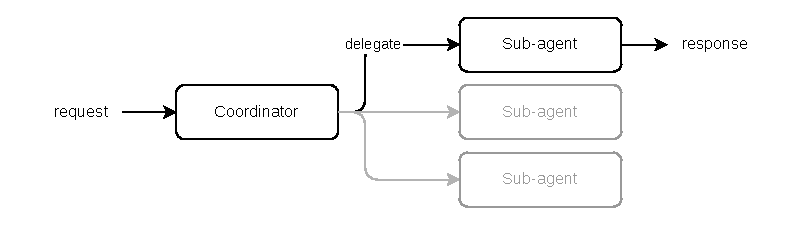
\includegraphics[width=0.9\textwidth]{images/routing_response_direct.pdf}
	\caption[Direct response]{Delegation. The selected sub-agent returns its response straight to the requester; the coordinator does not see it.}
	\label{fig:routing-direct}
\end{figure}

\begin{figure}[ht]
	\centering
	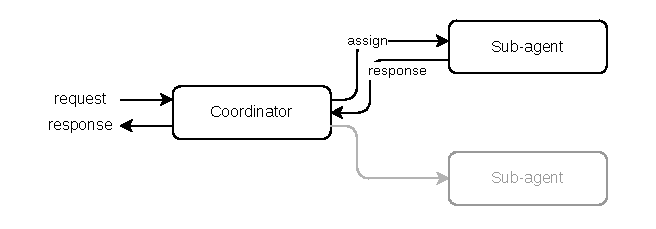
\includegraphics[width=0.74\textwidth]{images/routing_response_coordinator.pdf}
	\caption[Coordinator-mediated response]{Assignment. The selected sub-agent returns its response to the coordinator, which elaborates the final response sent to the requester.}
	\label{fig:routing-coordinator}
\end{figure}

\subsection{Separable and overlapping specialization}
\label{subsec:separable-overlapping}

What the routing decision has to resolve depends on how the sub-agents relate to each other. The sub-agents may cover disjoint subject matter, and in this case the wording of a request separates them. A support system with a billing agent and a shipping agent is of this kind: a request that mentions an invoice or a refund belongs to the billing agent, and a request that mentions a package or a delivery date belongs to the shipping agent. The two agents rarely share vocabulary, so the classification is straightforward from the text alone.

By contrast, in other systems the sub-agents may cover the same subject matter, or subject matters that are closely related. In this case, the wording of a request becomes harder to map to the right one. A travel-booking system with an agent dedicated to the lowest fare and a separate agent dedicated to the shortest travel time is of this kind: both agents can receive a request about the same flight, and the wording of the request might not, by itself, indicate which of the two constraints the requester meant to prioritize.

The same effect is documented in intent classification. ATIS and SNIPS are two datasets of task-oriented dialog utterances. Each utterance is labeled with its \emph{intent class}, the category of goal it expresses, such as \emph{flight} or \emph{airfare} \cite{bihaniFuzzyClassificationMultiintent2021}. Bihani and Rayz compared classification accuracy across the two and reported that it depends on the lexical overlap between the classes \cite{bihaniFuzzyClassificationMultiintent2021}. In ATIS, phrases such as \emph{show me} and \emph{from} repeat across different intent classes; accuracy on it is lower and more variable than on SNIPS, where utterances of different intents share fewer words \cite{bihaniFuzzyClassificationMultiintent2021}. They gave the utterances \emph{show me flights to Philadelphia coming from Baltimore}, labeled as the intent \emph{flight}, and \emph{show me airlines with flights from Denver}, labeled as the intent \emph{airline}, as an example of this overlap \cite{bihaniFuzzyClassificationMultiintent2021}. Higher lexical overlap between the classes lowers the accuracy with which an utterance is mapped to the correct one. This is the same difficulty that a coordinator faces when the sub-agents that it selects among cover overlapping subject matter, as in the fare and travel-time example above.

This extends to multi-turn scenarios. In conversational systems, a request is not necessarily self-contained: the element that fixes which sub-agent should handle it can appear in an earlier turn rather than in the last one. The context relevant to the routing decision is then spread across turns alternated between the user and the assistant, which adds the task of gathering that context to the difficulty of overlapping vocabulary described above.

\subsection{Downstream dependence on the routing decision}
\label{subsec:downstream-dependence}

The coordinator is the causally earliest step of the coordinator pattern described above, and the only one whose output determines which other component runs at all. Once the request has been handed to a sub-agent, no later step reopens the selection. An error made by the coordinator is therefore inherited by everything computed after it. The sub-agent applies its own criteria to a request that should have been handled under different criteria, and its output can be internally consistent while still addressing the wrong problem.

A wrong routing decision is therefore a problem of \emph{trajectory}: the correctness of a run is a property of the whole sequence of steps, and a wrong step early in it is not repaired by anything that follows. It is one instance of a broader problem in evaluating agents, discussed in Chapter~\ref{chap:evaluating-agents}.


\chapter{Evaluation of LLMs and LLM-based Agents}
\label{chap:evaluating-agents}

The performance measure of Section~\ref{subsec:rationality} drives action selection during the run of a classical agent, since the decide step selects the action expected to maximize it. An LLM-based agent has no such measure active during the run. It is not built for one task, and its objective is stated in the prompt as natural language.

Whether the behavior obtained matches the behavior intended is decided only after the run, by an evaluation setup that defines both what to check and how to check it. That criterion is applied to the text an LLM-based agent produces as output, but also to the trajectory one or more LLM-based agents may produce while pursuing their goal. This chapter reviews how that criterion is constructed, first for the language model as the core agent component, then for the LLM-based agent built on top of it. It also reviews the additional evaluation problems that construction introduces.

\section{Text Matching and Benchmarks}
\label{sec:text-matching-benchmarks}

\subsection{Text Matching}
\label{sec:text-matching}

Scoring a language model's output against a predetermined reference text is the earliest form of automatic evaluation for generated text. This is a natural language generation problem, not one specific to agents or large language models: any system that produces text needs a way to be scored against a reference. BLEU and ROUGE are the traditional metrics for this problem. BLEU compares a generated translation to one or more reference translations through a weighted average of n-gram precision, matched phrase by phrase against the reference \cite{papineniBleuMethodAutomatic2002}. ROUGE applies the same surface-level comparison to summarization, counting overlapping n-grams, word sequences, or word pairs between a generated summary and human-written reference summaries \cite{linROUGEPackageAutomatic2004}. Both metrics reduce evaluation to how closely the generated text matches a reference text, and this reference-based comparison was shown to correlate poorly with human judgment, particularly on tasks that require creativity and diversity \cite{liuGEvalNLGEvaluation2023}.

\subsection{Benchmarks as Capability Exams}
\label{sec:benchmarks-capability-exams}

A benchmark of a large language model is a set of tasks chosen to represent a capability, together with a standardized procedure for running every model on those tasks and a metric for scoring each one. The result is packaged into a leaderboard so that models can be compared under the same protocol \cite{liangHolisticEvaluationLanguage2023}. Running a model on a task requires an \emph{adaptation} procedure. Adaptation is the method that turns a general-purpose language model into a solver for that one task, for example a specific prompting strategy \cite{liangHolisticEvaluationLanguage2023}. The comparison across models is meaningful only if every model is evaluated on the same scenarios and adapted to each task by the same procedure; otherwise, a difference in score can come from the adaptation method rather than from the model itself \cite{liangHolisticEvaluationLanguage2023}. A benchmark may score an output with text-matching metrics such as BLEU and ROUGE, or apply a different metric when the task requires checking something other than how closely the output resembles a reference string.

MMLU (Massive Multitask Language Understanding) is a benchmark of this kind, on a task where the answer is a single choice. It is a multiple-choice test built from 57 subjects across the humanities, sciences, and other domains, and each item is scored by classification accuracy on the selected answer choice \cite{hendrycksMeasuringMassiveMultitask2021}. The correct answer is one of a predetermined set of options, so the model is scored by whether it selects the option matching the key, not by any comparison of generated text against a reference string.

BFCL (Berkeley Function Calling Leaderboard), another benchmark, illustrates the same point as MMLU for a task where the answer is not text at all: the metric fits the kind of answer the task produces. It evaluates a model's ability to produce function calls and scores them through abstract-syntax-tree sub-string matching, used as a proxy for executing the call: a function call is correct if the function name matches exactly and every parameter value falls within its allowed range \cite{patilBerkeleyFunctionCalling2025}. A function call is a structured object, not a string to be compared word by word, so the benchmark checks its syntactic structure and argument values instead of applying a text-matching metric to it. MMLU and BFCL score two different kinds of output, classification accuracy on a predetermined answer choice and structural correctness on a generated call, and in both cases the metric is chosen to fit what the task is asking.

This benchmark model presupposes headroom: the leaderboard has to separate models by capability, which requires that the tasks not already be solved by every model under test.

\section{Benchmark Saturation}
\label{sec:benchmark-saturation}

The benchmark Humanity's Last Exam is introduced on the observation that the headroom MMLU relies on has closed: language models have now exceeded 90\% accuracy on popular benchmarks such as MMLU, which limits how much such a benchmark can still measure about state-of-the-art capability \cite{phanHumanitysLastExam2025}. Once most models under test score near the ceiling, the benchmark no longer separates them by capability, and the leaderboard collapses toward a narrow band of scores that no longer reflects differences in what the models can do.

Agent benchmarks report the same closing of headroom: top-performing agents have reached scores exceeding 90\% on existing benchmarks, which are becoming saturated and losing their ability to differentiate state-of-the-art agents \cite{guoSelfEvolvingBenchmarksSynthesizing2026}. Saturation is therefore a general property of predetermined benchmarks as models improve.

Benchmarks presuppose headroom: they separate models by capability only if the tasks are not already solved by every model under test. Headroom can close through mechanisms other than accumulated capability gains. Evaluation data can leak into training corpora, and fine-tuning on it inflates a model's score without a matching gain in capability \cite{akhtarWhenAIBenchmarks2026}. Benchmarks therefore need constant revision, proposing tasks difficult enough to preserve headroom \cite{akhtarWhenAIBenchmarks2026}.

Saturation is one way a predetermined evaluation stops discriminating between models. A second way is for the evaluation to be poorly matched to the domain it is applied to. One example is Singhal et al.'s work on medical question answering, where existing benchmarks are limited to classification accuracy or automated natural language generation metrics such as BLEU, and do not support the detailed analysis that real-world clinical use requires \cite{singhalLargeLanguageModels2023}. In place of such generic metrics, evaluation of clinical answers is carried out along axes specific to the domain, including factuality, comprehension, reasoning, possible harm, and bias \cite{singhalLargeLanguageModels2023}. A generic accuracy score or a generic text-generation metric does not capture what makes a clinical answer acceptable, so the metric is redefined around the domain instead of reused from a general-purpose benchmark.

A domain-tailored metric such as this one is still a single predetermined metric, applied to an output that is checked against a predetermined notion of what counts as acceptable. This is sufficient as long as the task itself has a comparison point of that kind. It stops being sufficient once the task is open-ended and has no predetermined answer to compare the output against, so that no single metric, however well matched to the domain, is left with anything to compare it to.

\section{Holistic Evaluation}
\label{sec:holistic-evaluation}

An open-ended or free-form generation task has no predetermined answer to compare its output against, so neither a predetermined-answer benchmark (Section~\ref{sec:benchmarks-capability-exams}) nor reference-based text matching (Section~\ref{sec:text-matching}) applies to it. The same limit applies to retrieval-augmented generation (RAG). RAG systems are commonly evaluated as extractive question answering, against datasets built around short extractive answers, but this does not represent how a RAG system is actually used, since it generates a synthesized answer rather than returning a predetermined span from the retrieved text \cite{esRagasAutomatedEvaluation2025}. As with open-ended generation, the output cannot be checked against a predetermined reference, so a different evaluation approach is needed.

The Holistic Evaluation of Language Models (HELM) responds to this by evaluating a model along several dimensions at once, rather than reducing it to a single score \cite{liangHolisticEvaluationLanguage2023}. Table~\ref{tab:helm-metrics} lists the seven metrics that HELM records for each scenario, with the property that each one measures \cite{liangHolisticEvaluationLanguage2023}.

\begin{table}[ht]
    \centering
    \renewcommand{\arraystretch}{1.2}
    \begin{tabularx}{0.85\textwidth}{@{}>{\raggedright\arraybackslash}p{2.2cm}X@{}}
        \toprule
        Metric & What it measures \\
        \midrule
        Accuracy & Task-specific correctness of the output, such as exact match or the F1-score against the expected response. \\
        Calibration & How closely the model's predicted confidence matches its actual rate of being correct. \\
        Robustness & Worst-case accuracy under small, meaning-preserving input perturbations, such as typos or paraphrases. \\
        Fairness & Disparity in accuracy across social groups, measured through counterfactual perturbations of group-related terms. \\
        Bias & Asymmetry in the language a model generates, such as skewed demographic representation or stereotyped associations. \\
        Toxicity & Rate of offensive, hateful, or otherwise harmful content in model generations, detected by an automated classifier. \\
        Efficiency & Computational cost of training and inference, including energy use, carbon emissions, and runtime. \\
        \bottomrule
    \end{tabularx}
    \caption[The seven metrics that HELM records for each scenario]{The seven metrics that HELM records for each scenario \cite{liangHolisticEvaluationLanguage2023}.}
    \label{tab:helm-metrics}
\end{table}

Holistic evaluation is defined around three elements, each instantiated concretely in HELM's own design \cite{liangHolisticEvaluationLanguage2023}:

\begin{itemize}
    \item \emph{Broad coverage.} A wide range of scenarios is included, while what is left out is explicitly acknowledged. A scenario is a triple of task, domain, and language that determines a concrete use case to evaluate against, for example summarization of news articles in English \cite{liangHolisticEvaluationLanguage2023}. HELM realizes broad coverage by defining a taxonomy of scenarios and metrics, narrowed down to a core set of 16 scenarios.
    \item \emph{Multi-metric measurement.} Several metrics are measured for each scenario, rather than one. HELM records all 7 metrics from Table~\ref{tab:helm-metrics} for each of the 16 core scenarios, so that metrics other than accuracy are not left out of the evaluation.
    \item \emph{Standardization.} HELM adapts every model to each of the 16 core scenarios through the same few-shot prompts.
\end{itemize}

HELM adds a fourth, separate design choice on top of the core scenario and metric grid: \emph{targeted evaluations}, additional scenarios that isolate one skill or risk at a time, covering linguistic understanding, world and commonsense knowledge, reasoning, memorization and copyright, disinformation generation, bias, and toxicity generation \cite{liangHolisticEvaluationLanguage2023}.


\section{LLM-as-a-Judge}
\label{sec:llm-as-judge}

Each of HELM's 7 metrics from Section~\ref{sec:holistic-evaluation} is computed against a reference the scenario determines in advance. HELM's own evaluation includes two scenarios with no such reference: judging whether a generated headline or social media post supports a given thesis. None of the 7 metrics can be computed for these, so HELM falls back to human annotators recruited on Amazon Mechanical Turk, with each output rated by three workers, because no established automated evaluation exists for disinformation \cite{liangHolisticEvaluationLanguage2023}. Scoring an open-ended output therefore requires an \emph{oracle} in place of a predetermined reference string: a procedure that returns a verdict, given a candidate output, on whether it is a good answer. HELM uses a human rater for this case; a human rater is one such oracle, but human rating at scale is costly and could lead to poor repeatability. Using a language model as a reference-free evaluator has since been proposed by a growing body of work as a scalable alternative to a human rater \cite{liuGEvalNLGEvaluation2023}: instead of a human, a language model reads the candidate output and produces a verdict on its quality, standing in for the human rater or for a task-specific score function. This approach is named LLM-as-a-judge, and the model performing the grading is the judge.

\subsection{Grading Modes and the Reliability Question}
\label{sec:llm-as-judge-reliability}

Zheng et al. define three ways the judge can be used \cite{zhengJudgingLLMasaJudgeMTBench2023}:

\begin{itemize}
    \item \emph{Pairwise comparison}: the judge reads two candidate responses to the same prompt and states which one is better, or declares a tie.
    \item \emph{Single-answer grading}: unlike in pairwise comparison, the judge reads one response, with no other response to compare it against, and assigns it a score on a predetermined scale.
    \item \emph{Reference-guided grading}: the judge reads the candidate response together with a reference answer or a set of grading instructions, and scores the candidate against that reference.
\end{itemize}

Zheng et al. evaluate GPT-4 as a judge on two benchmarks built for this purpose: MT-Bench, a set of 80 multi-turn, open-ended questions spanning categories such as writing, reasoning, and coding, and Chatbot Arena, a crowdsourced platform on which users pose the same prompt to two anonymized models and vote for the response they prefer \cite{zhengJudgingLLMasaJudgeMTBench2023}. On these two benchmarks, GPT-4 agreed with human preference more than 80\% of the time, reaching 85\% on MT-Bench. The authors report this rate as matching, and on MT-Bench slightly exceeding, the 81\% agreement measured between two human annotators \cite{zhengJudgingLLMasaJudgeMTBench2023}. The result reads as evidence that a judge model can stand in for a human rater with little loss of reliability.

Reliability also depends on whether a judge's verdict is stable and free of bias. Shi et al. test this by evaluating fifteen LLM judges across MT-Bench and DevBench, a benchmark of software development tasks, over more than 150,000 evaluation instances \cite{shiJudgingJudgesSystematic2025}. Position bias is the tendency to favor a response because of its position in the comparison, such as being listed first, rather than because of its content. They report that position bias is both judge-dependent and task-dependent: the same judge model does not show the same degree of it across tasks, and different judge models rank differently on the same task \cite{shiJudgingJudgesSystematic2025}. Comparing judges against each other, rather than against human raters, they also find that judges with similar aggregate consistency scores frequently disagree on individual instances, with disagreement concentrated on cases where the candidate responses being compared are close in quality \cite{shiJudgingJudgesSystematic2025}. A bias or consistency figure reported for one judge on one benchmark therefore does not transfer to a different judge or a different benchmark without being measured again.

\subsection{G-Eval: A Framework for Building LLM-based Metrics}
\label{sec:llm-as-judge-geval}

Liu et al. propose G-Eval, not a single metric but a framework for building an LLM-based metric for a given evaluation criterion \cite{liuGEvalNLGEvaluation2023}. A G-Eval metric is assembled from a task introduction, a natural language instruction that states the task being evaluated, and a definition of the evaluation criterion, for example coherence in text summarization. The judge model expands these into its own chain-of-thought of evaluation steps before it is shown the candidate output and asked to score it \cite{liuGEvalNLGEvaluation2023}.

Reading a single score off the judge's output is unreliable in two ways that the authors report. First, one score value tends to dominate the distribution of outputs, which lowers the score's variance. Second, language models tend to return integer scores even when the prompt asks for decimal values, which produces ties that mask real differences between outputs \cite{liuGEvalNLGEvaluation2023}. G-Eval addresses both by reading the judge's probability distribution over the next token, at the position where the judge outputs its score. This is the same distribution over the vocabulary described in Section~\ref{subsec:unembedding}. From this distribution, only the probabilities of the tokens that denote a valid score value, such as the digits 1 to 5, are kept. The final score is the sum of each valid score value multiplied by its probability, rather than the single highest-probability token \cite{liuGEvalNLGEvaluation2023}. This turns a discrete, often-tied score into a continuous one, and is reported to raise the correlation with human judgment over the discrete version on the SummEval benchmark \cite{liuGEvalNLGEvaluation2023}.

With GPT-4 as the judge model, G-Eval reached an average Spearman correlation of 0.514 with human judgment on text summarization, averaged over four rated dimensions. This is a moderate correlation in absolute terms, but it is higher than the correlations reported for reference-based metrics such as ROUGE (0.192), embedding-based metrics such as BERTScore (0.225), and other LLM-based evaluators such as GPTScore (0.417) \cite{liuGEvalNLGEvaluation2023}. The authors report a systematic problem alongside this result: G-Eval assigns higher scores to GPT-3.5-generated summaries than to human-written ones, even in cases where human judges prefer the human-written summary, and attribute this to the judge favoring text similar to what it would generate itself \cite{liuGEvalNLGEvaluation2023}. Building a more accurate scoring function does not remove this kind of systematic deviation from human judgment; the next section places it within a broader taxonomy of such deviations.

\subsection{Systematic Biases in LLM-Judge Verdicts}
\label{sec:llm-as-judge-biases}

The literature has organized systematic deviations from human judgment into a taxonomy of biases. Ye et al. identified twelve named bias types, each a way the judge's verdict can shift for reasons unrelated to the quality of the response being graded \cite{yeJusticePrejudiceQuantifying2024a}. Table~\ref{tab:llm-judge-biases} lists all twelve, with a description of each.

\begin{table}[ht]
    \centering
    \renewcommand{\arraystretch}{1.2}
    \begin{tabularx}{0.9\textwidth}{@{}>{\raggedright\arraybackslash}p{3.4cm}X@{}}
        \toprule
        Bias & Description \\
        \midrule
        Position bias & Favoring a response for the position it occupies in a pairwise comparison, rather than its content. \\
        Verbosity bias & Favoring a longer response independently of its quality. \\
        Compassion-fade bias & Judging the same content differently depending on whether the responses are attributed to named models. \\
        Bandwagon bias & Favoring a response after being told it is the majority or popular choice. \\
        Distraction bias & Being swayed by content in the response that is irrelevant to the criterion being graded. \\
        Fallacy-oversight bias & Failing to penalize a response that contains a logical fallacy. \\
        Authority bias & Favoring a response that cites sources or authorities, regardless of whether the citation supports the claim. \\
        Sentiment bias & Favoring a response for its emotional tone rather than its content. \\
        Diversity bias & Judging content differently depending on demographic or cultural markers present in it. \\
        Chain-of-thought bias & The judge's own evaluation accuracy changes depending on whether it is prompted to reason step by step before returning a verdict. \\
        Self-enhancement bias & Favoring a response the judge model itself, or a model similar to it, is more likely to have produced. \\
        Refinement-aware bias & Judging a response differently once it is known to be a revision of an earlier one. \\
        \bottomrule
    \end{tabularx}
    \caption[The twelve bias types identified in LLM-as-a-judge verdicts]{The twelve bias types Ye et al. identify in LLM-as-a-judge verdicts \cite{yeJusticePrejudiceQuantifying2024a}.}
    \label{tab:llm-judge-biases}
\end{table}

Two of these have been studied as specific cases on their own.
\begin{itemize}
	\item Position bias: Shi et al. found that its strength depends on the quality gap between the two responses compared: the closer the two responses are in quality, the more the judge's verdict is affected by which position each response occupies \cite{shiJudgingJudgesSystematic2025}.
	\item Self-enhancement bias, referred to by Wataoka et al. as self-preference: they reported that GPT-4, used as a judge, exhibits a significant degree of self-preference, and attributed this to language models favoring text that is more familiar to them, including text that the model itself, or a model similar to it, is more likely to have produced \cite{wataokaSelfPreferenceBiasLLMasaJudge2025}.
\end{itemize}

Relative to the reference-based metrics of Section~\ref{sec:text-matching-benchmarks}, an LLM judge can grade an output for which no predetermined reference exists, since the judge substitutes for the reference rather than requiring one. This is what makes it applicable to open-ended generation. The cost of this flexibility is exposure to the biases described above. A reference-based metric scores one output at a time against its predetermined reference string, so the position of a response in a comparison cannot affect its score. It also does not generate text itself, so it cannot favor a response for resembling its own output, unlike a judge model. An LLM judge reads the full context of the comparison, so it is exposed to signals that the grading task was not meant to depend on. The rate of this exposure depends on the judge model, the task, and the grading mode, so it must be measured for the specific setting the judge is deployed in, not assumed from a bias rate reported in a different study.


\section{The Agent Evaluation Problem}
\label{sec:agent-evaluation-problem}

An agent's task-solving process consists of a sequence of states, not a single output, which raises the question of what counts as the right unit of evaluation once the subject is an agent. The classical rational agent, introduced in Section~\ref{subsec:rationality}, offers a starting point for this question. Its behavior is evaluated by a performance measure, external to it and predetermined before it runs \cite[Chap.~2]{russellArtificialIntelligenceModern2022}.

\subsection{Same Outcome, Different Trajectories}
\label{subsec:quadratic-example}

Scoring the agent's behavior by its effect on the environment, rather than by the behavior itself, is the starting point for the example in Figures~\ref{fig:quadratic-tool} and \ref{fig:quadratic-direct}.

\begin{problembox}
  Two agents are given the equation $x^2 - 4 = 0$ and asked to report the values of $x$ that satisfy it.
\end{problembox}

\begin{scenariobox}{Scenario A}
  The agent calls a math tool, which solves the equation and returns the roots, as shown in Figure~\ref{fig:quadratic-tool}.

  \begin{figure}[H]
    \centering
    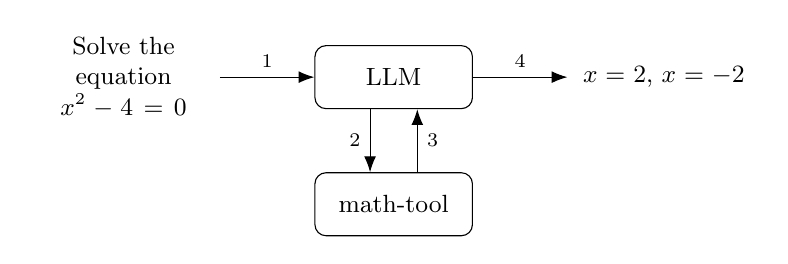
\begin{tikzpicture}[
        node distance=12mm,
        every node/.style={font=\small},
        box/.style={draw, rounded corners, align=center, minimum height=8mm, minimum width=20mm},
        arr/.style={-{Latex[length=2mm]}}
        ]
        \node[align=center, text width=22mm] (query) {Solve the equation\\$x^2-4=0$};
        \node[box, right=of query] (llm) {LLM};
        \node[align=center, text width=22mm, right=of llm] (output) {$x=2$, $x=-2$};
        \node[box, below=8mm of llm] (tool) {math-tool};
        \draw[arr] (query) -- (llm) node[midway, above] {\scriptsize 1};
        \draw[arr] ([xshift=-3mm]llm.south) -- ([xshift=-3mm]tool.north) node[midway, left] {\scriptsize 2};
        \draw[arr] ([xshift=3mm]tool.north) -- ([xshift=3mm]llm.south) node[midway, right] {\scriptsize 3};
        \draw[arr] (llm) -- (output) node[midway, above] {\scriptsize 4};
    \end{tikzpicture}
    \caption[Tool-call trajectory]{Tool-call trajectory.}
    \label{fig:quadratic-tool}
  \end{figure}
\end{scenariobox}

\begin{scenariobox}{Scenario B}
  The agent produces the roots directly, because the underlying language model has been trained on equations of this form and predicts the result without an intermediate step, as shown in Figure~\ref{fig:quadratic-direct}.

  \begin{figure}[H]
    \centering
    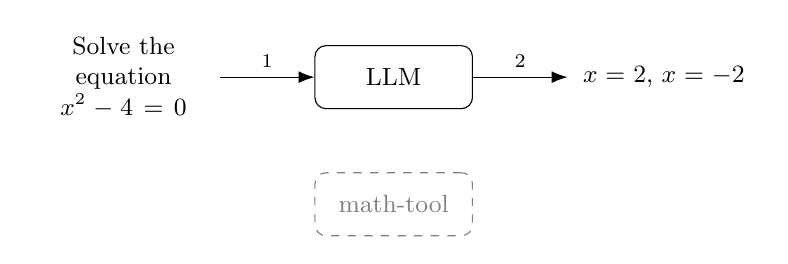
\begin{tikzpicture}[
        node distance=12mm,
        every node/.style={font=\small},
        box/.style={draw, rounded corners, align=center, minimum height=8mm, minimum width=20mm},
        unusedbox/.style={draw, dashed, rounded corners, align=center, minimum height=8mm, minimum width=20mm, text=gray, draw=gray},
        arr/.style={-{Latex[length=2mm]}}
        ]
        \node[align=center, text width=22mm] (query) {Solve the equation\\$x^2-4=0$};
        \node[box, right=of query] (llm) {LLM};
        \node[align=center, text width=22mm, right=of llm] (output) {$x=2$, $x=-2$};
        \node[unusedbox, below=8mm of llm] (tool) {math-tool};
        \draw[arr] (query) -- (llm) node[midway, above] {\scriptsize 1};
        \draw[arr] (llm) -- (output) node[midway, above] {\scriptsize 2};
    \end{tikzpicture}
    \caption[Direct-response trajectory]{Direct-response trajectory.}
    \label{fig:quadratic-direct}
  \end{figure}
\end{scenariobox}

Both scenarios report $x = 2$ and $x = -2$. An outcome-only criterion, applied to the final answer alone, scores them identically, because it has no access to the process that produced the answer and therefore cannot distinguish an answer produced by a tool call from one produced directly by the model. The two trajectories differ, however, in the guarantee they carry beyond this single equation. Scenario A routes equations to the same deterministic solver, so a harder or less common equation is handled by the same computation and solved with the same reliability. Scenario B carries no such guarantee: the model can produce incorrect roots for a harder or less common equation with the same confidence with which it reports the correct ones here.

\subsection{Outcome-Only Evaluation in Coding Benchmarks}
\label{subsec:coding-benchmarks-outcome-only}

Coding benchmarks that evaluate agents on software engineering tasks do not all treat the trajectory the same way: some score an agent purely by outcome, as in Scenario A and Scenario B above, while others also account for how that outcome was reached, and the choice determines what the benchmark measures. SWE-bench and ViBench, reviewed below, are outcome-only in their primary metric. SWE-bench scores an agent's submission by applying the proposed patch to the repository and running the associated test suite: a task instance is resolved when the patch applies and all tests pass, and the reported metric is the percentage of task instances resolved \cite{jimenezSWEbenchCanLanguage2024a}. This metric excludes the tool calls that the agent makes while producing the patch, their order, and the intermediate observations returned by the repository or the test runner. It reads only the final patch and the pass or fail outcome of the tests.

ViBench, a more recent coding benchmark, sharpens the same separation. Its primary score, Pass@1, credits an artifact only when every test plan associated with it scores full marks, indicating the absence of bugs or missing functionality \cite{zhongViBenchBenchmarkVibe2026a}. A test plan is a natural-language script of browser interactions that a human end user or QA tester would perform. Pass@1 verifies the running application's behavior through this browser automation, evaluated independently of the source code \cite{zhongViBenchBenchmarkVibe2026a}. The agent's tool-use trajectory is not part of this score: it is examined afterward, through what the benchmark calls \emph{trajectory-level} and \emph{qualitative failure-mode} analyses, presented separately from and after the Pass@1 and graded-score results \cite{zhongViBenchBenchmarkVibe2026a}. ViBench names this separation explicitly, treating trajectory analysis as a distinct, secondary step rather than a component folded into the metric. This separation may follow from a constraint on generic benchmark design. Trajectory analysis presupposes access to an agent's internal architecture. Because that architecture differs across the agents a benchmark evaluates, trajectory analysis cannot be standardized into a single metric the way an outcome check on the produced artifact can. This makes explicit the property that SWE-bench's design leaves implicit: the score reads only the outcome the agent produces. The process that produced it is analyzed, when it is analyzed at all, outside the scoring procedure.

\section{Trajectory-aware Evaluation}
\label{sec:trajectory-aware-evaluation}

Trajectory-aware evaluation scores the sequence of intermediate steps that an agent takes, its tool calls, plans, and decisions, rather than only the final output, and responds to the gap described in Section~\ref{sec:agent-evaluation-problem}.

The gap is not limited to trajectories that differ in whether a tool is invoked. It appears also between two agents that both use a tool: one agent can solve the equation with a single call to a symbolic math tool, while another can reach the same roots through multiple calls, applying a sequence of algebraic transformations and a general formula for the roots of a polynomial where the single call would have applied the specific formula for a quadratic. Both agents report $x = 2$ and $x = -2$, and an outcome-only criterion scores them identically. The two trajectories differ in the number of tool calls and in the computation that each call carries out, which affects the cost of the run. More generally, the correctness of the output is not sufficient to establish that the process producing it was carried out correctly. That has to be checked at the level of the trajectory itself.

Trajectory-aware evaluation is not a single method. Mohammadi et al.\ organized agent evaluation along two axes \cite{mohammadiEvaluationBenchmarkingLLM2025}:

\begin{itemize}
    \item \emph{What is evaluated}: outcome-oriented agent behavior, on one side, against process-oriented agent capabilities on the other, such as tool use, planning and reasoning, memory and context retention, and multi-agent collaboration.
    \item \emph{How the evaluation is carried out}: the interaction mode, the data, the metrics, and the tooling involved.
\end{itemize}

Within this taxonomy, the metrics and evaluation strategies that fit a given case depend on what is being assessed \cite{mohammadiEvaluationBenchmarkingLLM2025}. AgentBench, $\tau$-bench, and TRAJECT-Bench illustrate this variation with three concrete instances of trajectory-aware evaluation. All three target process-oriented capabilities, but they differ along the second axis of the taxonomy, the interaction mode used to elicit and score the trajectory, so each scores a different aspect of the agent's process:

\begin{itemize}
    \item \emph{AgentBench} evaluates agents across eight distinct environments, task settings such as an operating system shell, a database, and a knowledge graph, each with its own action space and metric \cite{liuAgentBenchEvaluatingLLMs2025}. The agent interacts with each environment over multiple turns, with the number of rounds ranging from five to thirty-five, so the benchmark assesses reasoning and decision-making across the interaction rather than at a single output.
    \item \emph{$\tau$-bench} measures an agent's ability to interact with a simulated user and with programmatic APIs while following a domain-specific policy document \cite{yao$t$benchBenchmarkToolAgentUser2024}. Its reward combines two terms: whether the database state, the content of the records the agent's tool calls wrote or changed, matches an annotated target state, and whether the agent's responses to the user adhere to the policy. The score thus depends on how the agent conducted the interaction, not only on the state it left behind.
    \item \emph{TRAJECT-Bench} reports trajectory-level diagnostics alongside final accuracy, including the correctness of tool selection and of the arguments passed to each tool, and whether dependencies and ordering constraints between steps are satisfied \cite{heTRAJECTBenchTrajectoryAwareBenchmark2025}.
\end{itemize}


\section{The Multi-Agent Trace}
\label{sec:multi-agent-trace}

The evaluation methods surveyed in Section~\ref{sec:trajectory-aware-evaluation} score a single agent's trajectory: its sequence of intermediate steps, tool calls, plans, and decisions. This framing does not cover what happens once several agents work together, as described in Chapter~\ref{chap:agents}. In a multi-agent system, agents exchange messages along a given topology. A single agent's trajectory records only that agent's own steps, so it captures neither the messages exchanged with other agents nor the topology they flow along. Evaluating such a system therefore requires a concept broader than a single trajectory, called the \emph{trace}, which consists of every participating agent's trajectory, the inter-agent messages exchanged between them, and the topology along which those messages and outputs flow. Trajectory-aware evaluation, as scoped in Section~\ref{sec:trajectory-aware-evaluation}, accounts for the first component of the trace; it does not account for the second and third.

Cemri et al. studied failures of multi-agent LLM systems using this broader concept, the execution trace, rather than individual agent trajectories \cite{cemriWhyMultiAgentLLM2025a}. Working from a set of traces produced by running multi-agent systems on their target tasks, they analyzed an initial set of 150 traces and derived from it a taxonomy of failure modes, the Multi-Agent System Failure Taxonomy (MAST) \cite{cemriWhyMultiAgentLLM2025a}. The taxonomy was then validated by annotating a larger set of 1642 traces against its failure modes, with inter-annotator agreement reported for the labeling procedure \cite{cemriWhyMultiAgentLLM2025a}. MAST groups 14 distinct failure modes into three categories \cite{cemriWhyMultiAgentLLM2025a}:

\begin{itemize}
    \item \emph{System Design Issues}: failures that originate from system design decisions, and from poor or ambiguous prompt specifications.
    \item \emph{Inter-Agent Misalignment}: failures that arise from a breakdown in the flow of information between agents during execution, such as a failure to share information, a misinterpretation of another agent's output, or a departure from an agreed task specification.
    \item \emph{Task Verification}: failures that involve inadequate verification of the final output, including no or incomplete verification, incorrect verification, or terminating the task before it is complete.
\end{itemize}

Inter-agent misalignment accounted for over 30\% of observed failures across the annotated set of 1642 traces \cite{cemriWhyMultiAgentLLM2025a}, and it is distinct from the other two categories, which are attributable to the design of a single agent or to the absence of a verification step. Since these failure modes are properties of the messages exchanged between agents and not of any single agent's trajectory, they are only visible when the trace is the object under evaluation.

\section{Failure Attribution}
\label{sec:failure-attribution}

The taxonomy in Section~\ref{sec:multi-agent-trace} names a failure mode but does not indicate which agent or which step in the trace caused it. Failure attribution is the additional task of assigning a trace failure to the agent and step responsible for it, so that a fix can target that agent or step rather than the run as a whole.

\subsection{Attribution Methods}
\label{sec:attribution-methods}

Zhang et al. formulated this step and introduced Who\&When, a benchmark of 127 annotated multi-agent systems in which each failed trace is labeled with the agent and the step responsible for the failure \cite{zhangWhichAgentCauses2025}. The automated methods that they evaluate on this benchmark are themselves built on the LLM-as-a-judge paradigm of Section~\ref{sec:llm-as-judge}, applied here to read a failure trace and return a verdict on who is responsible instead of grading a single output \cite{zhangWhichAgentCauses2025}. Against this benchmark, the best of these methods reached 53.5\% accuracy at identifying the responsible agent and 14.2\% accuracy at pinpointing the responsible step, and some methods performed below random on the step-level task \cite{zhangWhichAgentCauses2025}. The gap between the two figures indicates that identifying which agent is at fault is considerably easier than identifying at which point in that agent's trajectory the fault occurs. The low step-level accuracy is a further instance of the judge unreliability already established in Section~\ref{sec:llm-as-judge}, here applied to a harder task, reading a failure trace instead of grading a single response. These methods are trained and evaluated against the 127 traces in Who\&When. Labeling a trace at this granularity (agent and step) by hand is costly, which limits how much attribution data of this kind can exist.

AgenTracer targets this labeling cost: it automates the annotation of failed multi-agent trajectories through counterfactual replay and programmed fault injection, rather than relying on traces labeled by hand \cite{zhangAgenTracerWhoInducing2025}. Fault injection here means taking a trajectory that succeeded and deliberately corrupting one of its actions, so that the resulting failure has a known cause by construction \cite{zhangAgenTracerWhoInducing2025}. A tracer trained on the traces that the AgenTracer pipeline produces outperformed large proprietary judges, including Gemini-2.5-Pro and Claude-4-Sonnet, by up to 18.18\% on the Who\&When benchmark \cite{zhangAgenTracerWhoInducing2025}.

Both Who\&When's judges and AgenTracer's automated labels treat attribution as the selection of one responsible agent and one responsible step, a single ground truth to predict. DoVer questioned this framing and approached attribution as intervention-driven debugging instead: it generates a hypothesis about the responsible agent and step, then verifies the hypothesis through targeted interventions on the trace, in the same spirit as AgenTracer's fault injection but applied to check a hypothesis rather than to generate training data, such as editing a message or altering a plan, rather than accepting the hypothesis on its own \cite{maDoVerInterventionDrivenAuto2026}. The authors observed that framing attribution as the search for a single responsible agent and step is often ill-posed, since multiple distinct interventions can independently repair the same failed task \cite{maDoVerInterventionDrivenAuto2026}. In et al. reported the same difficulty from a different angle: existing benchmarks and methods largely assume a single deterministic root cause, but multi-agent system failures often admit multiple plausible attributions because of complex inter-agent dependencies and ambiguous execution trajectories \cite{inRethinkingFailureAttribution2026}. A trace failure, in this view, is not always reducible to one agent and one step; more than one attribution can be defensible for the same run.

\subsection{Cost of Attribution}
\label{sec:cost-of-attribution}

Attribution methods of the kind surveyed above need a complete trace to reason over, and reasoning over the trace once is often not enough: both AgenTracer and DoVer establish the responsible agent and step by replaying the trace under a modification rather than by reading it once. AgenTracer produces its labels through counterfactual replay combined with programmed fault injection \cite{zhangAgenTracerWhoInducing2025}, and DoVer replays each trial with an intervention applied in-situ, running three independent replays per intervention and, across the four settings it evaluates, between 1.4 and 4.0 replay trials per case \cite{maDoVerInterventionDrivenAuto2026}. Producing an attribution this way therefore implies two things. First, it requires re-executing part or all of the trace multiple times. Each replay checkpoints the state it starts from, and the procedure repeats until a hypothesis is confirmed. This adds a compute cost on top of whatever was already spent producing the original trace, and the cost scales with the number of interventions or fault injections a method tries before it converges on an attribution. Second, replaying a trace requires the trace to already exist in full: the run must have finished before any replay, checkpoint, or intervention can be performed on it. Attribution of this kind is therefore an offline procedure, carried out after the run is complete, and its cost in money and time is paid only after a failure has already happened. This implies a distinction between offline evaluation, performed on a completed trace, and online evaluation, performed during execution, developed in Section~\ref{sec:offline-online-evaluation}.


\section{Offline and Online Evaluation}
\label{sec:offline-online-evaluation}

\subsection{Definitions and Feedback Loop}
\label{sec:offline-online-definitions}

Xia et al. distinguished two stages at which a check can run, offline and online, and described evaluation-driven development and operations (EDDOps), an approach that places the two within a single closed feedback loop rather than treating them as alternatives \cite{xiaEvaluationDrivenDevelopmentOperations2025}. In EDDOps, offline and online evaluation results both feed a shared analysis step, which drives either a bounded runtime adjustment or a governed offline redevelopment. A redevelopment change is then re-verified with offline evaluation on the same cases before it reaches the live system \cite{xiaEvaluationDrivenDevelopmentOperations2025}.

\begin{itemize}
    \item \emph{Offline evaluation} runs against a predetermined suite of tasks or logged trajectories, on a subset of cases, ahead of release.
    \item \emph{Online evaluation} runs against live traffic, continuously, while the system operates in deployment.
\end{itemize}

A predetermined offline suite covers only a limited slice of the conditions a system meets after deployment. Xia et al. made the same point: predetermined suites cover a limited slice of possible tasks and inputs, so they are less likely to surface issues that emerge with changing data, tools, or user behavior \cite{xiaEvaluationDrivenDevelopmentOperations2025}. Online evaluation catches what the predetermined suite structurally cannot: conditions outside the suite, met only after deployment, such as emergent failures, drift, or violations of latency, cost, and availability targets \cite{xiaEvaluationDrivenDevelopmentOperations2025}.

\subsection{Security Evaluation}
\label{sec:security-evaluation}

Security is a further object of evaluation, and it motivates red-teaming, evaluation carried out by proactively attacking or testing a system to identify its vulnerabilities \cite{purpuraBuildingSafeGenAI2025}. Purpura et al. note that red-teaming is useful for an organization that wants to anticipate threats to its system and safeguard against them before production, but also that red-teaming alone does not guarantee the safety of a model after deployment, and recommend constant monitoring of a system once it is in production \cite{purpuraBuildingSafeGenAI2025}. Red-teaming therefore runs in both modes: an offline check performed once before release, and an online one run continuously against live traffic.

Purpura et al. distinguish red-teaming from guardrailing: red-teaming probes a system for vulnerabilities before deployment, and guardrailing safeguards the system after deployment \cite{purpuraBuildingSafeGenAI2025}. A guardrail is a check placed on a model's input or output, run online, that blocks a request or a response before it reaches the next step.

\subsection{Early Exit and the Feedback Loop}
\label{sec:early-exit-feedback-loop}

Running a check online, continuously, adds a capability an offline check cannot offer regardless of what it measures: the run can be stopped at the point the check fails, before the steps that would follow are executed. This is an alternative to the costly post-hoc attribution introduced in Section~\ref{sec:cost-of-attribution}: instead of reconstructing after the fact which step of a completed trace caused a failure, an online check identifies the failing step as it happens, and the run can exit there rather than run to completion. This early exit matters most for multi-agent systems and long trajectories. Without it, a run already known to have failed at one step would otherwise continue producing further steps, agent calls, and tool calls. The cost of those further steps is spent on a trajectory that cannot succeed. Stopping at the point of failure avoids this additional cost, and, since the state at that point is already checkpointed, the run can also be resumed or repaired from the failing step rather than discarded outright.

What happens after a check fails is decided by error handling, a step distinct from the check itself: the run is resumed from the checkpoint, repaired, or discarded, depending on the kind of failure that the check detected. Guardrailing is one instance of this pattern: it triggers the exit, and error handling determines the response that follows, such as refusing the request or returning a safe fallback.

This closes the loop described in Section~\ref{sec:offline-online-definitions}: evidence collected online about where and how a system fails is fed back to build the checks that later run online, so that a failure pattern identified once informs the check that catches and stops the same pattern the next time it occurs.


\section{Evaluating the Coordinator}
\label{sec:evaluating-coordinator}

The coordinator pattern of Section~\ref{sec:coordinator} fits the terms this chapter has built. The routing decision is a trajectory-level property in the sense of Section~\ref{sec:trajectory-aware-evaluation}: every sub-agent downstream of the coordinator acts on it, so a wrong routing decision is not repaired by anything that runs after it, regardless of how correctly that later step is carried out. The correctness of a run that involves a coordinator therefore cannot be read off the final output alone; it depends on whether the routing step itself was correct.

This also makes the routing decision an attribution target in the sense of Section~\ref{sec:failure-attribution}. Establishing that a run failed because of routing, rather than because of a later step, requires the same kind of attribution discussed there, with the same two limits: a judge cannot reliably confirm that a routing decision was wrong, and confirming it through replay requires the run to already be complete.

The offline and online regimes of Section~\ref{sec:offline-online-evaluation} both apply to the routing decision. Offline, routing decisions can be checked against a predetermined suite of requests with a known correct sub-agent. Online, a check on the routing decision offers a case of the early exit described in Section~\ref{sec:early-exit-feedback-loop}: a misrouting caught as the decision is made allows the run to be halted before any sub-agent acts on it, rather than allowing the run to complete on a request that was handed to the wrong sub-agent.

The experimental part of this work takes up the coordinator's routing decision under this framing.



\chapter{Research Scope and Requirements}
\label{chap:motivation}

Chapter~\ref{chap:evaluating-agents} illustrates why evaluating the coordinator's routing decision is hard, particularly when the goal is to catch a wrong decision before the coordinator delegates the request to a sub-agent. Section~\ref{sec:cost-of-attribution} shows that attributing a failure to a specific agent and step by inspecting a completed trace is costly and does not scale when performed by hand. Section~\ref{sec:failure-attribution} shows that automating this attribution with an LLM-as-a-judge is not much more reliable: on the Who\&When benchmark, the best automated method reached 53.5\% accuracy at identifying the responsible agent and 14.2\% accuracy at pinpointing the responsible step, with some methods scoring below random \cite{zhangWhichAgentCauses2025}.

A check that runs at the moment of the coordinator's decision, before the selected sub-agent is invoked, would attribute the failure to the coordinator itself and could prevent the rest of the trace from running. A source for that check could come from probing the hidden states of the coordinator's underlying LLM.

This chapter reviews the literature on hidden-state probing for routing decisions and identifies the gaps it leaves open. The chapter then determines the requirements that guide the rest of this work.

\section{Designs for a Routing Check}
\label{sec:routing-check-designs}

To attribute a wrong decision to the coordinator, and to prevent the wrong routing from taking effect, a check needs to be available before the coordinator invokes the selected sub-agent.

One option is a deterministic check, which applies a heuristic or a policy, encoded as a rule, over the request. Section~\ref{subsec:building-approaches} makes the same point about a hand-authored specification in general, in the context of classical agents. Writing it correctly demands domain expertise, and it is incomplete by construction, since it covers only the cases it was written to anticipate. A rule matched against a request is this kind of specification, so its coverage is bounded the same way, and it does not generalize across a sub-agent catalog it was not written for.

A language model can also serve as this check, reused as a judge that grades the coordinator's routing decision. As Section~\ref{sec:llm-as-judge} shows, a judge model carries systematic biases of its own. It also adds latency and cost, since it requires a separate model call for every decision it checks. Moreover, because the judge is itself an LLM performing a similar reasoning task, it is subject to the same class of failure as the coordinator it is meant to check.

A classifier trained to predict the correct sub-agent label from a fixed representation of the request's text can be a further source for evaluation. The representation is computed without the routing labels, and only the classifier that reads it is trained on them. This work refers to a classifier of this kind as a \emph{text-only classifier}. It can be trained on lexical features, counting how many times each word occurs in a query (a \emph{bag-of-words} representation), optionally weighted by how rare the word is across the training set using \emph{TF-IDF}. An alternative is a classifier trained on \emph{sentence embeddings}: dense vectors produced by an embedding model that capture the meaning of a sentence. In this case, two queries phrased differently but with the same meaning can map to nearby vectors. A text-only classifier of any of these three kinds can be more efficient than an LLM, and can also exceed a zero-shot LLM's accuracy on the same routing task \cite{balaMultiAgentRoutingSetValued2026}. However, this is not guaranteed: depending on the routing task, an LLM may perform better than a text-only classifier. Where a text-only classifier is more accurate than the coordinator's own LLM, its disagreement with the coordinator's decision could flag a likely misrouting, or the classifier could replace the coordinator's classification entirely, rather than only check it.

Wu, Zhu et al. showed that a probe, defined in Section~\ref{subsec:probing-method}, can capture a decision of this kind directly from a model's hidden states, with high accuracy: the tool a model is about to call is linearly encoded in its hidden states, and readable before the call is generated (Section~\ref{subsec:readability}) \cite{wuToolCallingLinearly2026}. A routing decision selects one sub-agent from a declared set, the same kind of selection that Wu, Zhu et al. studied for tool calls, so the information a check needs may already be present in the coordinator's hidden states before it generates a response. A probe trained on these hidden states could therefore be a stronger source than a text-only classifier for this decision, classifying the correct sub-agent directly from them and serving as an evaluation flag before the coordinator's decision takes place. However, this probe is beneficial only if its accuracy exceeds that of a text-only classifier: otherwise, it offers no advantage over a text-only classifier, which costs less to train and does not require access to hidden states.


\section{Related Work on Hidden-State Probing for Routing}
\label{sec:related-work-routing}

\subsection{Hidden State Probing for Routing and Evaluation}
\label{subsec:hidden-state-probing}

Hidden-state probing has been applied to classification tasks. One line of this work has focused on exploiting hidden states to choose which general-purpose LLM, from a fixed pool, should answer a query. Results report that a probe trained on the hidden states can outperform a classifier trained on the query's surface text.

Varshney et al. trained a probe on prefill activations, the hidden states from the forward pass over the prompt before generation starts, to predict, for each candidate model, its probability of answering a query correctly. The probe outperformed baseline classifiers built from sentence embeddings, retrieval, and text-complexity features, reaching a mean \emph{AUROC} (area under the ROC curve, a threshold-independent measure of how well a classifier ranks positive cases above negative ones) of 0.856 against 0.804 for the strongest baseline on the frontier model pool \cite{varshneyLLMRouterRethinking2026}.

Lugoloobi et al. reported the same pattern for a model's own success on mathematics and coding tasks: a probe trained on activations read before generation outperformed a TF-IDF baseline, with the margin ranging from 0.05 to 0.20 AUROC across models and tasks \cite{lugoloobiLLMsEncodeTheir2026}.

A separate study by Wu, Wang et al. found that a router trained on cross-layer hidden states outperformed routers built on output probabilities, embeddings, and verbose self-evaluation, for choosing between a local and a cloud model, with relative improvements of 16.68\% in AUROC and 18.86\% on the high-accuracy deployment scenario over the best baseline \cite{wuFairComprehensiveEvaluation2026}.

Reading a decision from the hidden states before generation has also been applied to tasks beyond choosing which model should answer.

Chen et al. built two classifiers on hidden states read during prompt prefill, to classify a prompt's topic as math, code, or general text: a trained linear probe, and a training-free classifier that reduces the hidden state to summary statistics and compares them to a reference statistic computed for each candidate topic. Direct LLM inference on this same task was less reliable than the trained probe, particularly for smaller models under zero-shot prompting: its accuracy improved only with larger models and in-context learning, needed careful prompt design to reach a reasonable level, and failed outright for the smallest model tested. The training-free classifier trailed the LLMs' own decisions on several cases, but generalized better to out-of-distribution and ambiguous prompts \cite{chenFastIntentClassification2025}.

Cencerrado et al. trained a linear probe on activations read after a question but before generation, to predict whether a model's own forthcoming answer would be correct. On out-of-distribution questions, the probe generalized better than an embedding-based baseline and a baseline built from \emph{verbalized confidence} (a confidence score the model states in its own text output), though the embedding-based baseline matched or slightly exceeded the probe on in-distribution questions \cite{cencerradoNoAnswerNeeded2026}.

Healy et al. trained a classifier on an agent's final-layer hidden states, taken from the same forward pass that generated a tool call. The classifier flagged whether that call hallucinated the wrong function, malformed its parameters, or bypassed the available tools, reaching up to 86.4\% detection accuracy \cite{healyInternalRepresentationsIndicators2026}.

Sun et al. trained a linear probe on an LLM's hidden state at the last input token, read before generation, to predict whether a task needs a tool call at all. The probe reached an AUROC of 0.89 to 0.96 across six models, exceeding the same models' own verbalized reasoning about tool necessity \cite{sunLLMAgentsAlready2026}.

Across the works reviewed in this subsection, hidden states carry information about a decision beyond what the model's own output reveals. Because this information is available before generation, a probe reading it may supply a signal that can be compared against the model's eventual output. This motivates using a probe as an evaluation mechanism that flags a routing error before it takes effect.

\subsection{LatentGate}
\label{subsec:latentgate}

Ratnakar et al. came closest to routing among specialized destinations with a hidden-state probe. LatentGate is a router that reads hidden states from a frozen small language model and classifies a query directly against a pool of specialized agents, to reduce the latency and cost of a prompt-based LLM router \cite{ratnakarLatentGateLowLatencySemantic2026}. The paper reports that a prompt-based LLM router takes 1,500 to 2,000 milliseconds per query, with cost scaling with the number of agents, against about 28 milliseconds for LatentGate, and estimates a 99.98\% reduction in the monthly cost of routing 1 million queries \cite{ratnakarLatentGateLowLatencySemantic2026}. LatentGate reaches this lower cost because it stops the forward pass at a fixed interior layer of the small language model and never generates output tokens. A linear probe then classifies the pooled hidden state at that layer into one of the candidate agents. The frozen model never receives the list of candidate agents, and it never receives a routing instruction. The query alone is tokenized and passed through the model, under a maximum sequence length of 128 tokens \cite{ratnakarLatentGateLowLatencySemantic2026}, so that its hidden states serve as a representation of the query for the probe to classify.

LatentGate is evaluated on its own synthetic benchmark of 100 enterprise agents, built so that agents in the same domain share vocabulary on purpose. On this benchmark's out-of-distribution queries, paraphrased and deliberately built to overlap in vocabulary with other agents, LatentGate reaches 80.0\% accuracy, against 60.0\% for a sentence-embedding classifier, BGE-M3 \cite{ratnakarLatentGateLowLatencySemantic2026}. Because the model is never instructed to route, its own routing accuracy is never measured, so the probe is never compared against the model it reads from. LatentGate attributes about 65\% of its own errors on its benchmark to the deliberate cross-domain vocabulary overlap \cite{ratnakarLatentGateLowLatencySemantic2026}, but the paper never reports the accuracy of a bag-of-words classifier on this benchmark, so whether such a classifier fails for the same reason, and by how much, is not established. The only such baseline that LatentGate reports is on CLINC150, a separate 150-class intent-classification benchmark. There, LatentGate outperforms an SVM and TF-IDF classifier by 1.7 percentage points, 92.9\% against 91.2\% \cite{ratnakarLatentGateLowLatencySemantic2026}. The small accuracy difference suggests that most of the routing signal on that benchmark is already recoverable from surface text, so the probe's contribution is limited. LatentGate's scope is also limited to single-turn queries \cite{ratnakarLatentGateLowLatencySemantic2026}.

\subsection{What the Literature Leaves Open}
\label{subsec:literature-gap}

The hidden-state probing work reviewed in Section~\ref{subsec:hidden-state-probing} and Section~\ref{subsec:latentgate} evaluates every probe on single-turn queries. None of it tests whether a hidden-state probe still routes correctly once a query follows more than one turn of conversation. Furthermore, none of it compares a probe's routing accuracy against the model's own routing accuracy, the comparison that defines a probe's effectiveness as an evaluation mechanism.

As Section~\ref{subsec:latentgate} shows, LatentGate is the reviewed work closest in approach, but its purpose differs, because it produces the routing decision instead of checking a decision the coordinator has already made. It is also the only one that builds its benchmark to be hard for a sentence-embedding classifier, by giving agents in the same domain overlapping vocabulary on purpose, and then attributes its own errors to that overlap. It does not run the same check for a bag-of-words classifier. LatentGate's scale also differs from a coordinator's: it routes among 100 agents, not the roughly three to seven a production coordinator typically selects among, as Section~\ref{sec:multi-agent} shows. At that scale, a classifier can fail because there are many candidates to choose among, not because any two are hard to tell apart. LatentGate's benchmark does not establish whether the same difficulty holds when the candidate pool is small and the only source of difficulty is overlap between a few agents.


\section{From the Literature Gap to the Research Questions}
\label{sec:rq-derivation}

Section~\ref{subsec:literature-gap} shows that no reviewed work evaluates a probe as an evaluation mechanism checked against the model's own decision, across both single-turn and multi-turn settings. Each research question below draws on one or more of these gaps.

\subsection{Probing as an Evaluation Mechanism}
\label{subsec:rq1-derivation}

\phantomsection\label{rq:rq1}
\begin{rqbox}[RQ1]
On requests where the correct sub-agent is difficult to determine from the wording alone, does a probe on the hidden states of a coordinator model recover the correct sub-agent more accurately than the coordinator's own selection?
\end{rqbox}


\noindent The probes reviewed in Section~\ref{sec:related-work-routing} either replace the routing decision outright, as LatentGate does, or check a model's own success on a task unrelated to routing, as Healy et al. and Cencerrado et al. do. None evaluates whether a probe can serve as a check on a coordinator's own routing choice, compared against the coordinator's own accuracy. The comparison targets requests where the wording does not determine the correct sub-agent. When the wording determines it, the probe's accuracy is explained by the request text, and the comparison against the coordinator does not isolate the contribution of the hidden states.

\subsection{Comparison with the Text-Only Classifiers}
\label{subsec:rq2-derivation}

\phantomsection\label{rq:rq2}
\begin{rqbox}[RQ2]
Does a probe on the coordinator's hidden states recover the correct sub-agent more accurately than classifiers trained on a fixed representation of the query text, such as raw word counts, TF-IDF weighting, or sentence embeddings?
\end{rqbox}


\noindent \hyperref[rq:rq1]{\textbf{RQ1}} compares the probe against the coordinator. This question compares the probe against the text-only classifiers, on the same requests. A probe can serve as an evaluation instrument only if it outperforms the text-only classifiers by a clear margin, on a dataset confirmed to be hard for those classifiers. Otherwise, a text-only classifier is sufficient.

\subsection{Consistency of the Optimal Layer}
\label{subsec:rq3-derivation}

\phantomsection\label{rq:rq3}
\begin{rqbox}[RQ3]
Does the optimal probe layer fall at a consistent relative depth across different LLMs?
\end{rqbox}


\noindent Comparing a probe against the coordinator and against the text-only classifiers requires training the probe at every layer of every model tested, since no single layer is known in advance to carry the routing decision best. This setup raises a further question: whether the best-performing layer falls at the same position across different models, or varies. The models tested differ in layer count, so the position is expressed as a fraction of network depth to make it comparable. If that relative depth is consistent, an evaluation probe could be trained on a fixed subset of layers, without a separate search to determine the optimal layer for each new model.

\subsection{Disagreement as a Misrouting Flag}
\label{subsec:rq4-derivation}

\phantomsection\label{rq:rq4}
\begin{rqbox}[RQ4]
Can the disagreement between the probe and the coordinator be used as a runtime flag for likely misrouting?
\end{rqbox}


\noindent This question asks whether the disagreement between the probe and the coordinator can serve as a runtime flag for likely misrouting. Such a flag could signal a trajectory likely to fail before the selected sub-agent runs. It could stop the run early, or prompt the coordinator to re-evaluate its routing choice in response to the disagreement.


\section{Requirements for a New Dataset}
\label{sec:dataset-requirements}

Answering the research questions defined in Section~\ref{sec:rq-derivation} requires both a single-turn and a multi-turn dataset. In this work, a \emph{sample} is a single data point of a dataset: one request, together with its target label. In both datasets, each sample must be a request meant to be submitted to a coordinator agent, which must route it to one of its available sub-agents. Each sample must also carry a target label, which defines the sub-agent to which the request must be routed. The rest of this section describes each requirement.

\subsection{Routing Task}
\label{subsec:routing-setup}

The number of sub-agents used must satisfy the following requirements.

\begin{itemize}
    \item It must stay within the range Section~\ref{sec:multi-agent} reports for a production coordinator, roughly three to seven sub-agents.
    \item It must allow requests for different sub-agents to share vocabulary, so that the wording alone does not reveal which sub-agent must handle the request.
\end{itemize}

Each sample must still be routable to one, and only one, sub-agent, so that a prediction on that sample can be marked right or wrong, depending on whether the chosen sub-agent matches the correct one. The shared vocabulary must therefore hold at the level of the wording, while the content of the request still selects a single sub-agent.

\subsection{Difficulty for Text-Only Classifiers}
\label{subsec:lexical-separability}

To answer \hyperref[rq:rq2]{\textbf{RQ2}}, the dataset must be challenging for text-only classifiers. This gives the probe margin to score above them.

Three text-only classifiers are used to measure how well this difficulty holds: a logistic regression trained on bag-of-words counts, a logistic regression trained on TF-IDF-weighted counts, and a logistic regression trained on sentence embeddings. The dataset must aim for the lowest accuracy these classifiers can reach, while every sample still reads as natural and remains routable to exactly one sub-agent, without an ambiguity that would leave it unroutable.

The sub-agents must also have a balanced number of requests, and be balanced in writing style, punctuation, and sentence pattern, in addition to vocabulary. Otherwise, a text-only classifier could route a request by its class frequency or by a stylistic marker instead of by what the request asks.

\subsection{Multi-turn Setting}
\label{subsec:multiturn-setting}

The multi-turn dataset must be built on the same sub-agents as the single-turn dataset, with the same writing styles, the same number of samples, and the same balance of samples across sub-agents. The only difference is that each multi-turn sample distributes its request across more than one turn, as defined in Chapter~\ref{chap:llm} (Section~\ref{subsec:query-prompt}), instead of stating it in one.

Each multi-turn sample must use the same number of turns, so that the length of the conversation is controlled. This count must stay fixed because the dataset is meant to show how performance changes between the single-turn and the multi-turn setting, not how it changes with the number of turns.

Each multi-turn sample must start with a request and end with a request. The final request must have no response: it is the request to be routed. Together, the turns in a sample are required to carry enough information to route the complete conversation to exactly one sub-agent.


\section{Requirements for Model Selection and Probing}
\label{sec:model-selection-requirements}

\subsection{Model Pool}
\label{subsec:model-pool-requirements}

\hyperref[rq:rq3]{\textbf{RQ3}} asks whether the best-performing layer falls at a consistent relative depth across different models. To answer this research question, data must be gathered from more than one LLM, from different model families and with different parameter sizes, from a few billion to several tens of billions. The pool of models must also satisfy the following requirements.

\begin{itemize}
    \item The models must vary in layer depth, so that models with more or fewer hidden layers can be compared. Layer depth is not fixed by parameter size alone: two models of similar size can stack a different number of layers, so depth is treated as a separate axis.
    \item Each model must be instruction-tuned, as described in Section~\ref{subsec:instruction-tuning}. This training is required for the model to read the dataset's routing prompt and return a routing decision, since the coordinator's own accuracy on this decision is one of the references that a probe is evaluated against, as Section~\ref{subsec:rq1-derivation} states.
    \item Each model must support tool calling, so that the coordinator can route the request to a sub-agent by invoking it as a tool.
    \item Each model must generate with sampling disabled (greedy decoding, described in Section~\ref{subsec:decoding}), so that its routing decision is deterministic and the run can be replicated.
\end{itemize}

Each model's weights must also be publicly available, so it can be run locally with a library such as Hugging Face's Transformers, which allows the model's hidden states to be read directly from the forward pass at every layer. A closed-source model, such as the models that OpenAI or Anthropic serve, is reached only through a network API. This API returns generated text and does not return the internal hidden states.

\subsection{Probe Input Position}
\label{subsec:probe-position-requirements}

Section~\ref{subsec:last-token} explains why the position a probe reads within the prompt matters. Most of the reviewed literature reads the hidden state at the last token of the prompt, before generation: this is the position used by Sun et al., by Cencerrado et al., and by Varshney et al., described in Section~\ref{subsec:hidden-state-probing}. LatentGate instead pools the hidden states over every token of the query \cite{ratnakarLatentGateLowLatencySemantic2026}.

This work reads hidden states from the last token of the prompt. Most of the reviewed literature reports good accuracy at this position, and reading only the last token is more efficient than probing every token of the query.

\subsection{Anisotropy and Whitening}
\label{subsec:anisotropy-scope}

At the center of LatentGate's method is a correction for anisotropy (Section~\ref{subsec:anisotropy}), applied through PCA-whitening before its probe is trained. This correction spreads the representations apart along the directions where they concentrate. It removes the shared component that makes representations of different classes look similar, which makes the classes easier for a linear probe to separate and raises its accuracy \cite{ratnakarLatentGateLowLatencySemantic2026}.

This work does not apply a whitening correction like LatentGate does, since raising the probe's peak accuracy is not a goal of this work. The classifier used as a probe is trained directly on the hidden states.


\chapter{Dataset Construction}
\label{chap:dataset-construction}

As determined in Section~\ref{sec:related-work-routing}, two synthetic datasets are generated to answer the research questions: one for single-turn requests, one for multi-turn requests. A large language model is prompted to generate the requests for a coordinator agent, each routable to exactly one of the available sub-agents. This chapter describes the design of these datasets, the pipeline that generates them, and the analysis used to validate them. Section~\ref{sec:dataset-overview} presents the taxonomy of sub-agents and the structure of a sample. Section~\ref{sec:generation-pipeline} describes the pipeline stages that produce the requests. Section~\ref{sec:dataset-baselines} and Section~\ref{sec:statistical-validation} report the baselines and the statistical analysis used to confirm that the dataset is suitable for the research questions.

\section{Sub-Agent Taxonomy and Sample Design}
\label{sec:dataset-overview}

Both the single-turn and the multi-turn dataset share the same taxonomy and are built around the same rationale. The only difference is that, in the multi-turn dataset, requests are composed of more than one turn.

In each of the two datasets, every request is chosen to describe a technical scenario in software engineering where a developer asks for guidance on a software system under construction or maintenance. Each request therefore belongs to the same domain and uses similar vocabulary, which responds to the requirement, stated in Section~\ref{subsec:lexical-separability}, that the dataset must be difficult for text-only classifiers. Requests from different domains would make lexical overlap harder to achieve, because the vocabulary would clearly separate the sub-agents: a request about a database migration and a request about a marketing campaign would share little vocabulary regardless of which sub-agent is correct, so their lexical overlap would be minimal and each request would be easily routable.

Software engineering is chosen, among other topics, because the author's familiarity with the domain makes manual review of the requests possible.

\subsection{Constraints}
\label{subsec:constraints-binding-waived}

Each request may express one or more \textbf{constraints}: technical demands that the software system under construction must satisfy, and constraints can conflict with each other. Each constraint is \textbf{owned} by exactly one of the available sub-agents: the constraint states a demand that falls within that sub-agent's concern.

An \textbf{authority figure}, a role named in the request such as a manager, a customer, or a regulator, determines the status of each constraint:

\begin{itemize}
    \item A constraint is \textbf{binding} when an authority figure imposes it. A binding constraint determines the correct sub-agent.
    \item A constraint is \textbf{waived} when an authority figure defers it, for example by moving it to a later milestone. A waived constraint remains part of the request, but it does not determine the correct sub-agent.
\end{itemize}

Exactly one constraint in a request is binding, and every other constraint it expresses is waived. The correct sub-agent is the sub-agent that owns the binding constraint. The sub-agent that owns a waived constraint is called the \textbf{decoy}. Section~\ref{subsec:constraints-example} gives an example of a request that expresses a binding and a waived constraint.

\subsection{Taxonomy}
\label{subsec:sub-agent-taxonomy}

Five sub-agents are used across the single-turn and the multi-turn dataset, within the range required in Section~\ref{subsec:routing-setup}. Table~\ref{tab:sub-agent-taxonomy} lists the five sub-agents and the concern each one owns. A request's correct sub-agent is the one pointed to by its binding constraint. Each sub-agent's name is followed by the identifier used to refer to it for the rest of this chapter.

\begin{table}[H]
    \centering
    \renewcommand{\tabularxcolumn}[1]{m{#1}}
    \begin{tabularx}{\textwidth}{@{}>{\raggedright\arraybackslash}m{6.2cm}>{\raggedright\hyphenpenalty=10000\exhyphenpenalty=10000\arraybackslash}X@{}}
        \toprule
        \textbf{Sub-agent} & \textbf{Binding constraint covered} \\
        \midrule
        \textbf{Scalable Architecture} \newline \texttt{scale\_arch} & Designing for concurrency, or for spreading the work across more machines, beyond the load the system carries today. \\ \addlinespace[0.9em]
        \textbf{Legacy Compatibility} \newline \texttt{legacy\_compat} & An existing API contract, client, or dependency that cannot change. \\ \addlinespace[0.9em]
        \textbf{Strict Regulatory Compliance} \newline \texttt{strict\_compliance} & A security, privacy, or regulatory rule. \\ \addlinespace[0.9em]
        \textbf{Resource Optimization} \newline \texttt{resource\_opt} & A fixed CPU, memory, or cost ceiling. \\ \addlinespace[0.9em]
        \textbf{Time-to-Market} \newline \texttt{time\_to\_market} & A fixed ship date or delivery deadline that cannot move. \\
        \bottomrule
    \end{tabularx}
    \caption[The five sub-agents and the binding constraint each one covers]{The five sub-agents and the binding constraint each one covers.}
    \label{tab:sub-agent-taxonomy}
\end{table}

\clearpage
\subsection{Example}
\label{subsec:constraints-example}

The following example illustrates a request that introduces a conflict between two constraints.

\begin{scenariobox}{Request}
\textit{``The events table and the reporting API share a connection pool today and it falls over under spikes. \binding{Our architect requires them separated into services with independent database access so instances scale out without contending for the same resources.} \waived{The analytics team would rather the API's response format stayed unchanged for existing clients, though they have agreed to a parallel-format window if we need to change it.} Where I would like input is the boundary itself: what belongs in the reporting service versus the events service, and how the read path crosses it.''}
\end{scenariobox}

\begin{table}[H]
    \centering
    \renewcommand{\tabularxcolumn}[1]{m{#1}}
    \begin{tabularx}{\textwidth}{@{}l>{\raggedright\hyphenpenalty=10000\exhyphenpenalty=10000\arraybackslash}X>{\raggedright\hyphenpenalty=10000\exhyphenpenalty=10000\arraybackslash}X@{}}
        \toprule
         & \textcolor{bindingcolor}{\textbf{Binding}} & \textcolor{waivedcolor}{\textbf{Waived}} \\
        \midrule
        \textbf{Constraint} & separate the events table and the reporting API into independently scaling services & keep the API's response format unchanged for existing clients \\ \addlinespace[0.9em]
        \textbf{Authority} & the architect & the analytics team \\ \addlinespace[0.9em]
        \textbf{Reason waived} & --- & agreed to a parallel-format window if the response format needs to change \\ \addlinespace[0.9em]
        \textbf{Owned by} & Scalable Architecture & Legacy Compatibility \\
        \bottomrule
    \end{tabularx}
\end{table}

As the example shows, a request can carry terminology for more than one sub-agent while only one of them is correct. A single binding constraint per request ensures exactly one correct sub-agent, the first requirement from Section~\ref{sec:dataset-requirements}, while the request still carries conflicting terminology.

\clearpage
\subsection{The Collision Graph}
\label{subsec:collision-graph}

Every pair of sub-agents carries a tension: a stated reason why their binding constraints conflict. With five sub-agents, ten pairs are possible, and Table~\ref{tab:collision-graph} lists all of them, from Section~\ref{subsec:sub-agent-taxonomy}, together with the tension each pair carries. The graph is complete: a collision is defined for every pair of sub-agents.

\vspace*{\fill}
\begin{table}[H]
    \centering
    \begin{tabular}{@{}ll>{\raggedright\hyphenpenalty=10000\exhyphenpenalty=10000\arraybackslash}m{9.5cm}@{}}
        \toprule
        \textbf{Sub-agent A} & \textbf{Sub-agent B} & \textbf{Tension} \\
        \midrule
        \texttt{time\_to\_market} & \texttt{scale\_arch} & Meeting the deadline can require hardcoding assumptions that break once the system has to handle far more load. \\ \addlinespace[0.9em]
        \texttt{time\_to\_market} & \texttt{resource\_opt} & Meeting the deadline can require spending more on compute or services than a fixed budget can cover. \\ \addlinespace[0.9em]
        \texttt{time\_to\_market} & \texttt{legacy\_compat} & Meeting the deadline can require changing or bypassing an existing contract that other clients still depend on. \\ \addlinespace[0.9em]
        \texttt{time\_to\_market} & \texttt{strict\_compliance} & Meeting the deadline can require skipping a security or privacy check that a regulation requires. \\ \addlinespace[0.9em]
        \texttt{scale\_arch} & \texttt{resource\_opt} & Scaling the architecture can require running more instances, which raises cost beyond a fixed budget. \\ \addlinespace[0.9em]
        \texttt{scale\_arch} & \texttt{legacy\_compat} & Scaling the architecture can require changing an interface that existing clients depend on. \\ \addlinespace[0.9em]
        \texttt{scale\_arch} & \texttt{strict\_compliance} & Scaling the architecture may require replicating data across more machines, which can move it outside a boundary that strict compliance requires it to stay within. \\ \addlinespace[0.9em]
        \texttt{resource\_opt} & \texttt{legacy\_compat} & Optimizing resources can require removing an abstraction layer, which changes a signature that existing clients depend on. \\ \addlinespace[0.9em]
        \texttt{resource\_opt} & \texttt{strict\_compliance} & Optimizing resources can require cutting a control, such as logging or encryption, that a regulation requires. \\ \addlinespace[0.9em]
        \texttt{legacy\_compat} & \texttt{strict\_compliance} & Preserving old behavior can require keeping a practice, such as an old data-handling method, that a new regulation no longer permits. \\
        \bottomrule
    \end{tabular}
    \caption[Ten colliding constraint pairs among the five sub-agents]{The ten colliding pairs among the five sub-agents, and the tension each pair carries.}
    \label{tab:collision-graph}
\end{table}
\vspace*{\fill}

\clearpage
\subsection{Difficulty Tiers}
\label{subsec:difficulty-tiers}

Samples are generated at three difficulty tiers. The tiers introduce the lexical difficulty required in Section~\ref{subsec:lexical-separability}.

\begin{itemize}
    \item \texttt{plain}: no collision. Only one constraint is stated, and it is binding, so nothing in the request competes with the correct sub-agent. A classifier or a probe is expected to score close to ceiling accuracy on this tier. A low accuracy score would point to a problem in how samples are generated or labeled, rather than to a hard routing decision.
    \item \texttt{natural}: a collision between two sub-agents, as in Table~\ref{tab:collision-graph}. The request talks about both constraints equally, and it says explicitly which one has been waived and by whom. A classifier is expected to score lower on this tier than on the \texttt{plain} tier, because the request also contains the vocabulary of a second sub-agent. An accuracy score equal to or higher than that of the \texttt{plain} tier would point to a waived constraint that is stated too weakly to compete with the binding one.
    \item \texttt{adversarial}: samples are built in pairs. The two requests of a pair share almost all their wording. They differ in only one short clause that names the constraint that has been waived. Each of the two requests names a different constraint as waived, so the pair's two correct sub-agents differ even though the requests are almost identical. A classifier is expected to score lower on this tier than on the \texttt{natural} tier, since most of the words it can use appear in both requests of a pair. An accuracy score equal to or higher than that of the \texttt{natural} tier would point to pairs whose requests differ in more than one clause, so that the remaining wording still identifies the correct sub-agent.
\end{itemize}

Within the \texttt{adversarial} tier, a pair is built around its decoy (Section~\ref{subsec:constraints-binding-waived}): the request presents the decoy's constraint, through its wording and emphasis, as if it were the binding one. The real binding constraint is still stated in the request, but it is written so that it is easy to miss. Four \emph{decoy patterns} are used to write the binding constraint this way, each applying only to the \texttt{adversarial} construction.

These patterns are designed to make routing harder for a coordinator model, not only for the text-only classifiers of Section~\ref{sec:dataset-baselines}.

In each example below, \binding{blue} marks the binding constraint.

\begin{itemize}
    \item \textbf{\texttt{buried\_rule}}: the request asks how to carry out one specific approach, for example a workaround. The binding constraint appears in only one clause of the request, and that clause states why the developer picked that approach instead of a simpler one.

    \begin{scenariobox}{Example -- \texttt{buried\_rule}}
    \textit{``We're trying to split the aggregate computation from the request handler so each can scale independently when we hit 10 million requests a day, though the infrastructure roadmap has that decoupling pushed out to next quarter, but \binding{the legacy API contract locks the response format to a specific JSON field at the top level and we have to keep it working.} Building around that constraint means the aggregation layer stays coupled to the response path. How do we handle the data flow here without rebuilding the response schema from scratch?''}
    \end{scenariobox}

    \item \textbf{\texttt{wrong\_cause}}: the request misleads on the cause of the problem. It confidently claims that the decoy constraint is the problem to be solved, and spends most of its words on it. The binding constraint appears only as a short fact, stated as if it were already obvious, with no explanation given.

    \begin{scenariobox}{Example -- \texttt{wrong\_cause}}
    \textit{``we're hitting memory ceiling hard on the cache, \binding{been blowing past the 512mb heap limit ops set,} and we keep trying to add smarter eviction policies and better compression to squeeze more in there, but the real problem is we can't reshape the response payload the way we need to because every mobile client and partner out there is hardwired to expect the exact json schema we published two years ago, though the api team cleared us to rework the output format if we have to. how do we get the instance footprint back under control without redesigning the whole data contract?''}
    \end{scenariobox}

    \item \textbf{\texttt{late\_mandate}}: the request is about the decoy constraint throughout. The binding constraint arrives at the end, in one flat-toned clause, so it reads as minor.

    \begin{scenariobox}{Example -- \texttt{late\_mandate}}
    \textit{``been looking at our read function design and we're spawning a helper thread for each request that comes in. works fine at current scale but the devops budget owner just locked us into a hard 512mb ceiling and max 64 threads, and they said we can revisit the threading model once we have more headroom in the budget. we have a bunch of production clients calling this function synchronously expecting it to block, and \binding{the platform arch team requires the function signature to stay exactly as-is.} so how do we actually redesign this without breaking the existing interface?''}
    \end{scenariobox}

    \item \textbf{\texttt{bad\_fix}}: the request misleads on the solution. It proposes a concrete fix that serves the decoy constraint, and asks for help carrying it out. The request also states the binding constraint, and that constraint is the reason the proposed fix does not work.

    \begin{scenariobox}{Example -- \texttt{bad\_fix}}
    \textit{``We're building a user profile cache that lives in process memory keyed by user id, and the product manager needs us to ship something working to early adopters in six weeks, with hardcoded cache sizes and TTLs acceptable to hit that deadline, but that timeline got pushed back in the roadmap review. At the same time, \binding{the operations team has set a hard ceiling of 512 megabytes of heap per instance for all caching and won't budge on that limit.} I'm proposing we start with simple fixed-size arrays and stop worrying about memory efficiency for now, which should get us there cheapest. How should we structure this to stay strictly within budget while keeping the implementation straightforward?''}
    \end{scenariobox}
\end{itemize}

\subsection{Personas}
\label{subsec:personas}

Four writing-style categories, called \emph{personas}, are used to generate a request. Personas exist to satisfy the requirement, from Section~\ref{subsec:lexical-separability}, that punctuation and phrasing styles stay balanced across sub-agents: assigning personas independently of the sub-agent prevents a sub-agent from being identifiable by a stylistic marker rather than by its content. Personas are assigned in equal proportions within every difficulty tier.

\begin{itemize}
    \item \textbf{\texttt{normal\_writing}}: the request reads as ordinary professional prose, written in complete sentences with correct punctuation.
    \item \textbf{\texttt{frustrated}}: the request reads as written by someone tired and irritated. Sentences are blunt, some sentences vent about the situation, and some sentences are incomplete, missing a subject or a verb.
    \item \textbf{\texttt{casual}}: the request reads as a relaxed chat message. It uses contractions, starts some sentences with a lowercase letter, and contains occasional small spelling or grammar mistakes.
    \item \textbf{\texttt{extremely\_casual}}: the request reads as a message typed in a hurry. It is mostly lowercase, uses minimal punctuation, and shortens words into abbreviations.
\end{itemize}

\subsection{Multi-turn Derivation}
\label{subsec:multiturn-derivation}

The multi-turn dataset uses a fixed number of turns, following the requirement in Section~\ref{subsec:multiturn-setting}. Every multi-turn sample starts with a developer message, and the developer and the coordinator then alternate messages. The conversation ends on a developer message, left unanswered, and the whole conversation is routed based on it. Together with the developer messages and the coordinator responses before it, this last message forms a fixed number of turns for every multi-turn sample. Conversation length therefore does not become a second difficulty axis alongside the three tiers. Each sample contains two full developer and coordinator turns, followed by the final, unanswered developer message, as Figure~\ref{fig:multiturn-alternation} shows.

\begin{figure}[H]
    \centering
    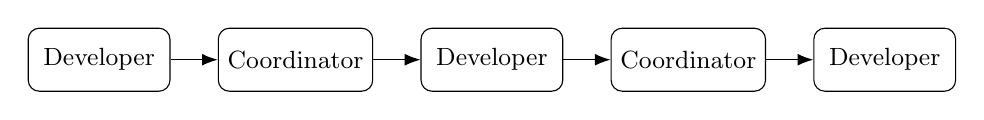
\begin{tikzpicture}[
        node distance=6mm,
        every node/.style={font=\small},
        box/.style={draw, rounded corners, align=center, minimum height=8mm, minimum width=18mm},
        arr/.style={-{Latex[length=2mm]}}
        ]
        \node[box] (d1) {Developer};
        \node[box, right=of d1] (c1) {Coordinator};
        \node[box, right=of c1] (d2) {Developer};
        \node[box, right=of d2] (c2) {Coordinator};
        \node[box, right=of c2] (d3) {Developer};
        \draw[arr] (d1) -- (c1);
        \draw[arr] (c1) -- (d2);
        \draw[arr] (d2) -- (c2);
        \draw[arr] (c2) -- (d3);
    \end{tikzpicture}
    \caption[Message alternation in a multi-turn sample]{Message alternation in a multi-turn sample.}
    \label{fig:multiturn-alternation}
\end{figure}

Single-turn constructions map to multi-turn ones directly: the same taxonomy, the same three difficulty tiers, the same personas and patterns, distributed across messages instead of stated once in a single message.

In a multi-turn adversarial pair, every message before the final one is identical, word for word, between the two members of the pair. The two requests differ only in the final, unanswered developer message, the same way the two requests of a single-turn adversarial pair differ only in one short clause. Figure~\ref{fig:multiturn-adversarial-fork} shows this shared prefix and the two final messages that follow it.

\begin{figure}[H]
    \centering
    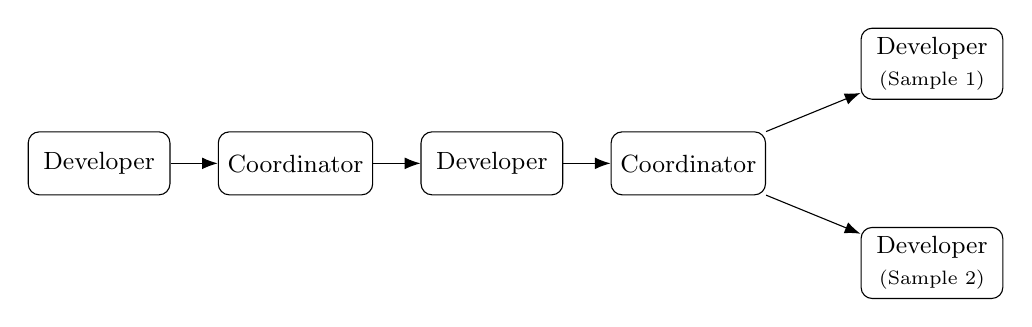
\begin{tikzpicture}[
        node distance=6mm,
        every node/.style={font=\small},
        box/.style={draw, rounded corners, align=center, minimum height=8mm, minimum width=18mm},
        arr/.style={-{Latex[length=2mm]}}
        ]
        \node[box] (d1) {Developer};
        \node[box, right=of d1] (c1) {Coordinator};
        \node[box, right=of c1] (d2) {Developer};
        \node[box, right=of d2] (c2) {Coordinator};
        \node[box, above right=4mm and 12mm of c2] (s1) {Developer\\\scriptsize (Sample 1)};
        \node[box, below right=4mm and 12mm of c2] (s2) {Developer\\\scriptsize (Sample 2)};
        \draw[arr] (d1) -- (c1);
        \draw[arr] (c1) -- (d2);
        \draw[arr] (d2) -- (c2);
        \draw[arr] (c2) -- (s1);
        \draw[arr] (c2) -- (s2);
    \end{tikzpicture}
    \caption[Shared prefix and final messages of a multi-turn adversarial pair]{Shared prefix and final messages of a multi-turn adversarial pair.}
    \label{fig:multiturn-adversarial-fork}
\end{figure}


\section{Generation Pipeline}
\label{sec:generation-pipeline}

Every sample is generated synthetically by prompting a large language model. The generation uses, for different tasks, Claude Haiku 4.5 and Claude Sonnet 5, both models provided by Anthropic. This section describes the stages that compose the generation pipeline, and discusses the sample count and distribution of the final single-turn and multi-turn datasets.

\subsection{Scenarios}
\label{subsec:scenarios}

Every request is grounded in a \textbf{scenario}: a short description of a software system under construction or under maintenance. The scenario set consists of 30 hand-authored scenarios. As the example below shows, a scenario describes only the system, with no sub-agent requests and no constraint, so a different binding constraint can be written for each of the five sub-agents from Section~\ref{subsec:sub-agent-taxonomy}, against the same scenario.

\begin{scenariobox}{Example -- scenario}
\textit{``An image processing routine converts every uploaded picture to a full-resolution intermediate representation in memory before applying any transformation.''}
\end{scenariobox}

\subsection{Facts}
\label{subsec:pipeline-facts}

For every scenario, a \textbf{fact} is generated for each sub-agent: one requirement on that system, owned by that sub-agent. The fact names the authority who imposes the requirement and what it demands. Each fact is generated with Claude Haiku 4.5. The example below shows two of the five facts drawn from the scenario in Section~\ref{subsec:scenarios}, one for \texttt{resource\_opt} and one for \texttt{legacy\_compat}.

\begin{scenariobox}{Example -- fact (\texttt{resource\_opt})}
\textit{``The cloud cost controller has capped monthly compute expenses at a fixed tier, which means the team must reduce the memory footprint of image processing by at least sixty percent from its current full-resolution approach to stay within budget without purchasing larger instances.''}
\end{scenariobox}

\begin{scenariobox}{Example -- fact (\texttt{legacy\_compat})}
\textit{``The published API contract guarantees that the image processing endpoint accepts files up to five gigabytes and returns the full intermediate representation upon request, so the team cannot change the in-memory storage behavior or response format without breaking existing client integrations.''}
\end{scenariobox}

\subsection{Sample Distribution}
\label{subsec:sample-distribution}

Generating one fact per sub-agent, for every scenario, yields 5 facts per scenario, 150 facts in total across the 30 scenarios. Since a request is generated from one or more facts, each stating one of its constraints, the number of available facts motivates the number of samples generated at each difficulty tier described in Section~\ref{subsec:difficulty-tiers}, and their distribution across sub-agents, reported in Table~\ref{tab:sample-distribution}.

\begin{table}[h]
    \centering
    \begin{tabular}{@{}lll@{}}
        \toprule
        \textbf{Tier} & \textbf{Per sub-agent} & \textbf{Total} \\
        \midrule
        \texttt{plain} & 30 & 150 \\
        \texttt{natural} & 120 & 600 \\
        \texttt{adversarial} & 180 & 900 \\
        \bottomrule
    \end{tabular}
    \caption[Sample counts per difficulty tier, single-turn and multi-turn]{Sample counts per difficulty tier, for each of the single-turn and multi-turn datasets.}
    \label{tab:sample-distribution}
\end{table}

The \texttt{plain} tier generates one request from each fact, stating that fact as the binding constraint. Every sub-agent owns 30 facts, one per scenario, so this gives 30 samples per sub-agent and 150 in total.

The \texttt{natural} tier generates one request from two facts, one for the binding constraint and one for the waived constraint. Swapping the two facts gives a different sample, since the binding fact sets the label. Every sub-agent is paired with each of its 4 colliding partners from Table~\ref{tab:collision-graph} in 30 samples, which gives 120 samples per sub-agent and 600 in total.

The \texttt{adversarial} tier builds pairs of requests instead of single requests: two facts are picked, and two requests are generated that share nearly all their wording, with a different one of the two facts stated as the binding constraint in each. The full design would pair every scenario with every one of the four decoy patterns from Section~\ref{subsec:difficulty-tiers}, for every colliding pair of sub-agents, and generate two requests per pairing. This would yield 2400 samples. Fewer are generated: 900 in total, 180 per sub-agent. This choice follows from budget: adversarial pairs are the most expensive samples to generate. The adversarial tier is set to 1.5 times the natural tier, so that the hardest tier is the largest in the dataset. Section~\ref{sec:dataset-baselines} confirms that the reduced number of adversarial samples does not affect the quality of the result.

\subsection{Plan}
\label{subsec:pipeline-plan}

The \textbf{plan} stage takes the sample counts fixed in Section~\ref{subsec:sample-distribution} and scaffolds every sample in the dataset. For each sample, it sets:

\begin{itemize}
    \item the sub-agent the sample must route to;
    \item the scenario it draws from and, within it, the fact that states this sub-agent's binding constraint;
    \item at the \texttt{natural} tier, the colliding sub-agent and the fact that defines its waived constraint;
    \item at the \texttt{adversarial} tier, the decoy sub-agent, the fact that defines its waived constraint, and the decoy pattern used to write it;
    \item the persona from Section~\ref{subsec:personas} that writes the request.
\end{itemize}

Every sub-agent has the same number of samples. Each scenario, persona, and decoy pattern also appears in the same number of samples for every sub-agent. This is the balance requirement that Section~\ref{subsec:lexical-separability} demands: without it, a sub-agent could be told apart by its sample count, its scenarios, or its writing style rather than by the constraint it owns. The scenarios, personas, decoys, and decoy patterns assigned to a sub-agent are shuffled separately, so that no scenario is always paired with the same persona, decoy, or decoy pattern.

The shuffle uses a fixed random seed, so it is deterministic: every run of the plan stage produces the same plan. Because the plan fixes every sample's design before any request is generated, the generation stage can be re-run multiple times, and each run generates only the samples that are still missing. This allows the dataset to be generated in parts instead of all at once, so that each part can be reviewed before the next one is generated. It also allows targeted regeneration: only the samples flagged by the audit stage (Section~\ref{subsec:pipeline-audit-repair}) are generated again.

\subsection{Generate}
\label{subsec:pipeline-generate}

The \textbf{generate} stage prompts a large language model for each sample, using the sample configuration the plan stage determined. The prompt asks for the text of the user message, or, for a multi-turn sample, the full conversation. Appendix~\ref{chap:appendix-prompts} reports all the prompts used.

The \texttt{plain} prompt instructs the model to treat one fact as the binding constraint. The \texttt{natural} prompt provides two facts and instructs the model to treat one as binding and the other as waived. The \texttt{adversarial} prompt provides two facts and the decoy pattern that the plan stage assigned. It instructs the model to write a pair of requests at once, following that pattern, so that the two requests share nearly all their wording and differ only in which fact is stated as binding. A multi-turn sample uses a separate prompt from its single-turn counterpart at the same tier, since it must render a conversation instead of one request.

An \texttt{adversarial} pair is generated in a single call, as one contrastive unit: the model is asked for both members of the pair together, so it keeps their shared wording close, instead of generating each member separately and risking a pair that does not overlap enough. For multi-turn samples, the two members of a pair share every turn up to, but not including, the last one: only the last turn differs between them, and it is this turn that carries the binding constraint.

Claude Haiku 4.5 was used to generate every request, except the multi-turn \texttt{adversarial} ones. For these, the audit stage (Section~\ref{subsec:pipeline-audit-repair}) flagged a large share of the samples generated with Claude Haiku 4.5. Manual inspection of the flagged samples, and repeated generation attempts, showed that the model could not reliably follow the constraints stated in its prompt for these requests, so Claude Sonnet 5 was used in its place.

\subsection{Audit and Repair}
\label{subsec:pipeline-audit-repair}

Once generation is complete, a set of checks is applied to every sample.

\paragraph{Structural Checks.} A request is checked against a length range, to catch a malformed generation, such as text cut short mid-sentence. A multi-turn sample is also checked to ensure that the turn alternation and the number of turns are correct, and every sample is checked for text that names one of the sub-agents directly, since a request that names its target gives the label away rather than letting it follow from the constraint.

\paragraph{Jaccard Index.} For an \texttt{adversarial} pair, the two members are checked for how much their words overlap. The check uses the Jaccard index \cite{nobleWhatJaccardSimilarity2026}, computed on the word sets $A$ and $B$ of the text that decides the label, for each of the two members:
\begin{equation}
    J(A, B) = \frac{|A \cap B|}{|A \cup B|}
\end{equation}
For a multi-turn pair, only the last user message is used, since Section~\ref{subsec:multiturn-derivation} makes it the only message that can differ between the two members. A pair whose two members share little wording is not contrastive: the label could be read off the surrounding text rather than the pivot that the pair is built around. The floor was set to 0.60 after a manual review of a subset of pairs. A pair whose Jaccard index falls below 0.60 is dropped, and the sample needs to be regenerated.

\paragraph{Oracle Check.} Claude Sonnet 5 is invoked as an oracle, for each generated request. It reads the request, with no view of the plan's intended sub-agent, and decides on its own which constraint is binding and which sub-agent owns it. This verdict, and the quote it is based on, are written back onto the sample and checked against the plan's intended sub-agent. The check confirms that the request carries enough information to route it to exactly one sub-agent, the requirement that Section~\ref{sec:dataset-requirements} states. A sample that the oracle flags, either because it disagrees with the plan or because it cannot decide, requires manual revision: it can be corrected by hand, marked as correct despite the oracle's verdict, or dropped so it can be regenerated.

A separate \texttt{repair} stage acts on the \texttt{regenerate} flag these checks set, whether from a failed check or from manual revision. It deletes every sample still carrying the flag, so the next \texttt{generate} run recreates it from the same plan row, without touching the plan or the samples that the checks did not flag. An \texttt{adversarial} pair is always regenerated as a whole: if one member is dropped, both are deleted and regenerated together, since a repaired half-pair could no longer be guaranteed to overlap with its twin the way that the Jaccard index check requires.

Figure~\ref{fig:pipeline-stages} shows the complete pipeline, from the scenario set to a checked sample, and the loop that a failed sample takes back to \texttt{generate}.

\begin{figure}[h]
    \centering
    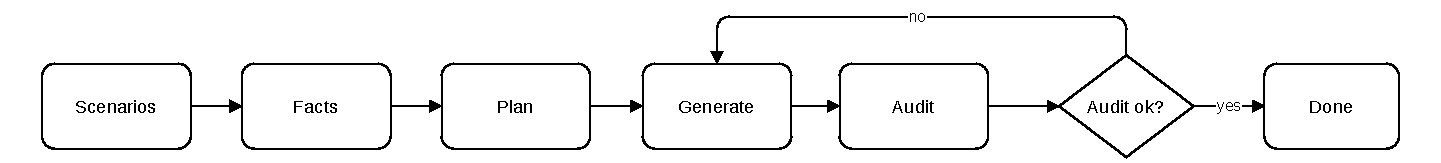
\includegraphics[width=\textwidth]{images/generation_pipeline.pdf}
    \caption[Generation pipeline, sample regenerated on audit failure]{The generation pipeline. A sample that fails the audit stage is regenerated.}
    \label{fig:pipeline-stages}
\end{figure}

\subsection{Cost}
\label{subsec:pipeline-cost}

Table~\ref{tab:pipeline-cost} reports the cost of producing both datasets, at Claude's Batch API prices, which halve the standard per-token rate. Each stage's figure is the total cost across every \texttt{generate} and \texttt{audit} iteration needed to reach the final set of samples, rather than the cost of a single pass. The \texttt{plan} and \texttt{facts} stages are not included: \texttt{plan} calls no model, and \texttt{facts} generates 150 short requests in total, a negligible cost next to the other stages.

\begin{table}[H]
    \centering
    \small
    \setlength{\tabcolsep}{3.5pt}
    \begin{tabular}{@{}llrrrrr@{}}
        \toprule
        & & \multicolumn{4}{c}{\textbf{Tokens (millions)}} & \\
        \cmidrule(lr){3-6}
        \textbf{Stage} & \textbf{Model} & \textbf{Input} & \textbf{Output} & \textbf{Cache read} & \textbf{Cache write} & \textbf{Cost} \\
        \midrule
        \texttt{generate}, single-turn            & Claude Haiku 4.5 & 4.32 & 0.61 & 0.00 & 0.00 & \$3.68 \\
        \texttt{generate}, multi-turn              & Claude Haiku 4.5 & 2.02 & 0.45 & 0.00 & 0.00 & \$2.15 \\
        \texttt{generate}, multi-turn \texttt{adversarial} & Claude Sonnet 5  & 1.49 & 1.44 & 1.40 & 2.34 & \$8.68 \\
        \texttt{audit}, single-turn                & Claude Sonnet 5  & 1.27 & 0.50 & 4.37 & 1.24 & \$3.78 \\
        \texttt{audit}, multi-turn                 & Claude Sonnet 5  & 2.38 & 0.53 & 4.77 & 1.23 & \$5.01 \\
        \midrule
        \textbf{Total} & & \textbf{11.47} & \textbf{3.53} & \textbf{10.54} & \textbf{4.81} & \textbf{\$23.30} \\
        \bottomrule
    \end{tabular}
    \caption[Tokens and cost for the single-turn and multi-turn datasets]{Tokens and cost of the run that produced the single-turn and multi-turn datasets, at Claude's Batch API prices. Input counts only the uncached input tokens.}
    \label{tab:pipeline-cost}
\end{table}


\section{Baselines}
\label{sec:dataset-baselines}

\subsection{Text-Only Classifiers}
\label{subsec:text-only-baselines}

Section~\ref{subsec:lexical-separability} requires the dataset to be difficult for classifiers that take only the request text as input, and it names three text representations that these classifiers must be trained on:

\begin{itemize}
    \item \textbf{bag-of-words}: a logistic regression over raw word counts (unigrams and bigrams);
    \item \textbf{TF-IDF}: a logistic regression over the same counts, weighted by TF-IDF;
    \item \textbf{sentence embeddings}: a logistic regression over sentence embeddings.
\end{itemize}

For each classifier, \emph{accuracy} is measured, given by
\begin{equation}
    \text{accuracy} = \frac{\text{requests classified correctly}}{\text{all requests}},
\end{equation}
where a request is classified correctly when the classifier's predicted sub-agent matches the correct sub-agent for that request.

Accuracy is measured with \emph{5-fold cross-validation}: the dataset is split into five folds, each classifier is trained on four folds and evaluated on the remaining fold, and this is repeated five times so that every fold serves once as the validation fold. Each fold, when it acts as the validation fold, produces a predicted sub-agent for every request in it. This is the \emph{out-of-fold prediction} for that request, since the request was never in the training data used to produce it. Collecting the out-of-fold prediction from each of the five folds gives one predicted sub-agent for every request in the dataset. Accuracy is then computed once, as defined above, by comparing each request's out-of-fold prediction against its correct sub-agent. This procedure uses every sample for both training and validation, without letting the same sample serve as both at once, and it prevents the reported accuracy from depending on one arbitrary split of the data. Folds are grouped by scenario, so a scenario's samples never split between the training fold and the validation fold. This matters for an \texttt{adversarial} pair, since its two requests share nearly all their wording: if one request were used for training and the other for validation, the classifier could match the validation request to its near-duplicate seen during training, and score high without learning to separate the sub-agents.

The sentence embeddings are obtained with \texttt{BAAI/bge-small-en-v1.5}, an embedding model that maps a request to a fixed-size vector encoding its meaning, so that requests with a similar meaning are mapped to nearby vectors.

Each classifier is trained and evaluated four times, on four different subsets of the samples:

\begin{itemize}
    \item \textbf{All}: the whole dataset;
    \item \textbf{Plain}: only the \texttt{plain} tier;
    \item \textbf{Natural}: only the \texttt{natural} tier;
    \item \textbf{Adversarial}: only the \texttt{adversarial} tier.
\end{itemize}

The accuracy obtained on both the single-turn and the multi-turn dataset is reported in Table~\ref{tab:text-baselines}.

\begin{table}[h]
    \centering
    \begin{tabular}{@{}l|lll|lll@{}}
        \toprule
        & \multicolumn{3}{c|}{\textbf{Single-turn}} & \multicolumn{3}{c}{\textbf{Multi-turn}} \\
        \textbf{Tier} & \textbf{Bag-of-words} & \textbf{TF-IDF} & \textbf{Embedding} & \textbf{Bag-of-words} & \textbf{TF-IDF} & \textbf{Embedding} \\
        \midrule
        Plain       & 0.900 & 0.993 & 0.927 & 0.840 & 0.987 & 0.873 \\
        Natural     & 0.708 & 0.730 & 0.653 & 0.665 & 0.677 & 0.592 \\
        Adversarial & 0.631 & 0.566 & 0.478 & 0.599 & 0.508 & 0.411 \\
        \midrule
        All         & 0.684 & 0.664 & 0.582 & 0.645 & 0.613 & 0.519 \\
        \bottomrule
    \end{tabular}
    \caption[Text-only classifier accuracy by difficulty tier, both datasets]{Accuracy of the three text-only classifiers, per difficulty tier, on the single-turn and the multi-turn dataset.}
    \label{tab:text-baselines}
\end{table}

On the whole dataset, no classifier reaches an accuracy above 0.69, on either the single-turn or the multi-turn dataset. Broken down by tier, accuracy falls from \texttt{plain} to \texttt{natural} and falls again from \texttt{natural} to \texttt{adversarial}, for all three classifiers, on both datasets. This is the decreasing accuracy that the tiers are designed to produce (Section~\ref{subsec:difficulty-tiers}). On \texttt{plain}, the request states only the binding constraint, so its vocabulary alone gives away the correct sub-agent. On \texttt{natural}, the request also states a waived constraint, so the vocabulary of a second sub-agent appears in the same request. On \texttt{adversarial}, the request is one half of a pair that shares nearly all its wording with its twin, so the words alone cannot tell which of the two constraints is binding.

The intrinsic difficulty of the \texttt{adversarial} design is also confirmed by the TF-IDF classifier results, which are outperformed by a non-TF-IDF-weighted bag-of-words classifier only on that tier, on both datasets. The two requests in an adversarial pair share nearly all their wording, and this high overlap makes TF-IDF down-weight words that still carry part of the routing signal.

The embedding classifier beats bag-of-words only on the \texttt{plain} tier. On \texttt{plain}, the request states one constraint, and the embedding captures it directly. On \texttt{natural}, the request also states a second, waived constraint. On \texttt{adversarial}, the request is nearly identical to its pair. In both cases, the embedding represents the whole request, and most of the request is the shared scenario text rather than the constraint that decides the sub-agent. Two requests built from the same scenario can then end up with similar embeddings even when they belong to different sub-agents, which lowers accuracy.

\subsection{Vocabulary and Routability}
\label{subsec:baseline-vocabulary}

Table~\ref{tab:baseline-terms} shows the single-turn TF-IDF terms with the highest weight, for each sub-agent. This confirms that most of the accuracy on \texttt{natural} and \texttt{adversarial} comes from requirement-specific vocabulary.

\begin{table}[h]
    \centering
    \begin{tabular}{@{}ll@{}}
        \toprule
        \textbf{Sub-agent} & \textbf{Highest-weighted TF-IDF terms} \\
        \midrule
        \texttt{legacy\_compat}     & contract, API, clients, existing, without breaking, published \\
        \texttt{time\_to\_market}       & weeks, working, demo, two weeks, ship, product \\
        \texttt{resource\_opt}      & memory, budget, ceiling, CPU, cloud, under \\
        \texttt{scale\_arch}        & scale, infrastructure, shared, horizontally, decouple, across \\
        \texttt{strict\_compliance} & audit, data, compliance, logging, security, officer \\
        \bottomrule
    \end{tabular}
    \caption[Highest-weighted TF-IDF terms per sub-agent]{Highest-weighted TF-IDF terms per sub-agent.}
    \label{tab:baseline-terms}
\end{table}

Section~\ref{subsec:lexical-separability} requires every request to stay routable to one sub-agent and to read as natural. The text-only baseline accuracies in Table~\ref{tab:text-baselines} are the lowest achievable under that requirement. To lower this accuracy further, the highest-weighted terms in Table~\ref{tab:baseline-terms} could be banned from generation, so that the generator cannot rely on them. The result is that the generator relies on synonyms instead, and a synonym is equally separable for a classifier. Banning every synonym as well introduces ambiguity: requests stop reading as natural and become hard to route even for a human.

\subsection{Difficulty Beyond the Baselines}
\label{subsec:encoder-robustness}

The generation pipeline is designed to minimize the accuracy of the three baselines whose results are reported in Table~\ref{tab:text-baselines}. Their low accuracy therefore does not show that the datasets are also difficult for other text-only classifiers. To show this, two more logistic regressions are trained on the representations of two different encoders, on the same scenario-grouped folds (Table~\ref{tab:modernbert-baseline}).

\begin{table}[H]
    \centering
    \small
    \begin{tabular}{@{}l|cc|cc@{}}
        \toprule
        & \multicolumn{2}{c|}{\textbf{Single-turn}} & \multicolumn{2}{c}{\textbf{Multi-turn}} \\
        \textbf{Tier} & \textbf{ModernBERT} & \textbf{BGE-M3} & \textbf{ModernBERT} & \textbf{BGE-M3} \\
        \midrule
        Plain       & 0.827 & 0.967 & 0.747 & 0.940 \\
        Natural     & 0.665 & 0.770 & 0.607 & 0.643 \\
        Adversarial & 0.552 & 0.524 & 0.462 & 0.431 \\
        \midrule
        All         & 0.618 & 0.654 & 0.541 & 0.555 \\
        \bottomrule
    \end{tabular}
    \caption[ModernBERT-large and BGE-M3 accuracy by difficulty tier]{Accuracy of the logistic regressions over ModernBERT-large representations and over BGE-M3 sentence embeddings, per difficulty tier, on the single-turn and the multi-turn dataset.}
    \label{tab:modernbert-baseline}
\end{table}

The first is trained on the representations of ModernBERT-large \cite{warnerSmarterBetterFaster2024}. ModernBERT-large maps each token of the request to a vector, and the representation of the request is obtained by mean pooling these vectors. The second is trained on the sentence embeddings of \texttt{BAAI/bge-m3}, a larger embedding model than \texttt{BAAI/bge-small-en-v1.5}.

Neither classifier reaches an accuracy above 0.69 on the whole dataset, single-turn or multi-turn, and the accuracy of both falls from \texttt{plain} to \texttt{natural} to \texttt{adversarial}, as for the three baselines. The difficulty is therefore a property of the datasets and is not specific to the three classifiers chosen as baselines.


\section{Statistical Analysis of Surface Features}
\label{sec:statistical-validation}

Section~\ref{subsec:lexical-separability} requires the sample set to be balanced across sub-agents in writing style, punctuation, and sentence pattern, not only in vocabulary. Without that balance, a text-only classifier could route a request by a stylistic marker instead of by what the request asks. This section reports an analysis of variance (ANOVA) that tests whether the dataset meets that requirement, over measurable \emph{surface features} of the request text, properties that define how a request is written, such as its length or its punctuation, computed directly from the characters and words of the request text.

\subsection{Design Factors}
\label{subsec:design-factors}

Every test in this section reads one or more of the following design factors:

\begin{itemize}
    \item \texttt{gold}: the correct sub-agent the request should be routed to.
    \item \texttt{decoy}: the sub-agent whose constraint is stated but waived, defined only when the sample carries a decoy.
    \item \texttt{difficulty}: the difficulty tier the sample was built at, \texttt{plain}, \texttt{natural}, or \texttt{adversarial} (Section~\ref{subsec:difficulty-tiers}).
    \item \texttt{pattern}: the decoy pattern used to write the adversarial pair, defined only for the \texttt{adversarial} tier (Section~\ref{subsec:difficulty-tiers}).
    \item \texttt{persona}: the writing style used to generate the request (Section~\ref{subsec:personas}).
\end{itemize}

\subsection{Sample Balance}
\label{subsec:sample-balance}

ANOVA assumes \emph{homoscedasticity}, that is, that the variance of the tested feature is the same in every group the factors define. Section~\ref{subsubsec:levene-kruskal} tests this assumption directly and finds it violated for several features. The F-test that ANOVA relies on is expected to remain robust to unequal variance when the design is balanced, that is, when every group holds the same number of samples \citep{glassConsequencesFailureMeet1972}.
This robustness is why the balance checked in this section matters beyond precision: it is also what keeps every ANOVA in this chapter valid despite the violated homoscedasticity assumption.

An unbalanced design also risks a different problem: an ANOVA can attribute variance to a factor that only occurs more often for one sub-agent, rather than to a real effect of that factor. The plan stage provides balanced samples by design (Section~\ref{subsec:pipeline-plan}), and Figure~\ref{fig:sample-balance} plots the sample counts that result.

\begin{figure}[H]
    \centering
    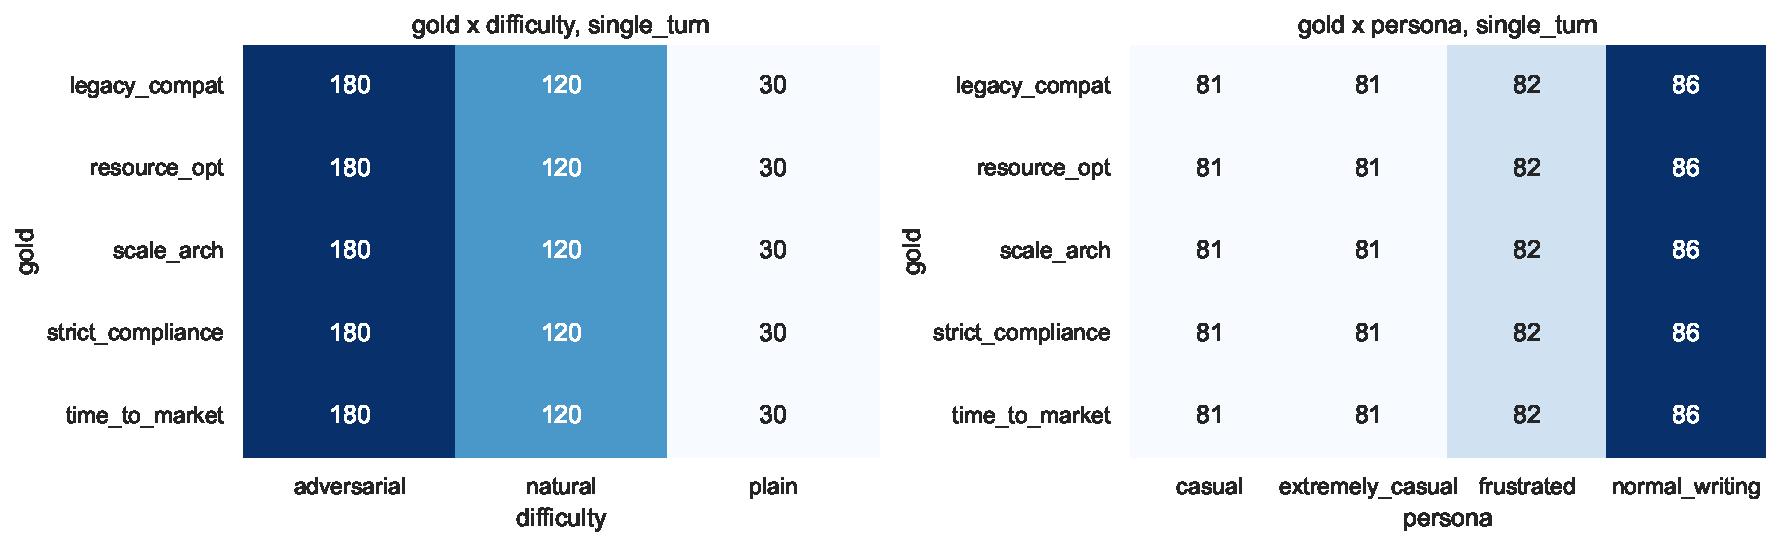
\includegraphics[width=\textwidth]{images/plots/anova/dataset_composition_single_turn.pdf}
    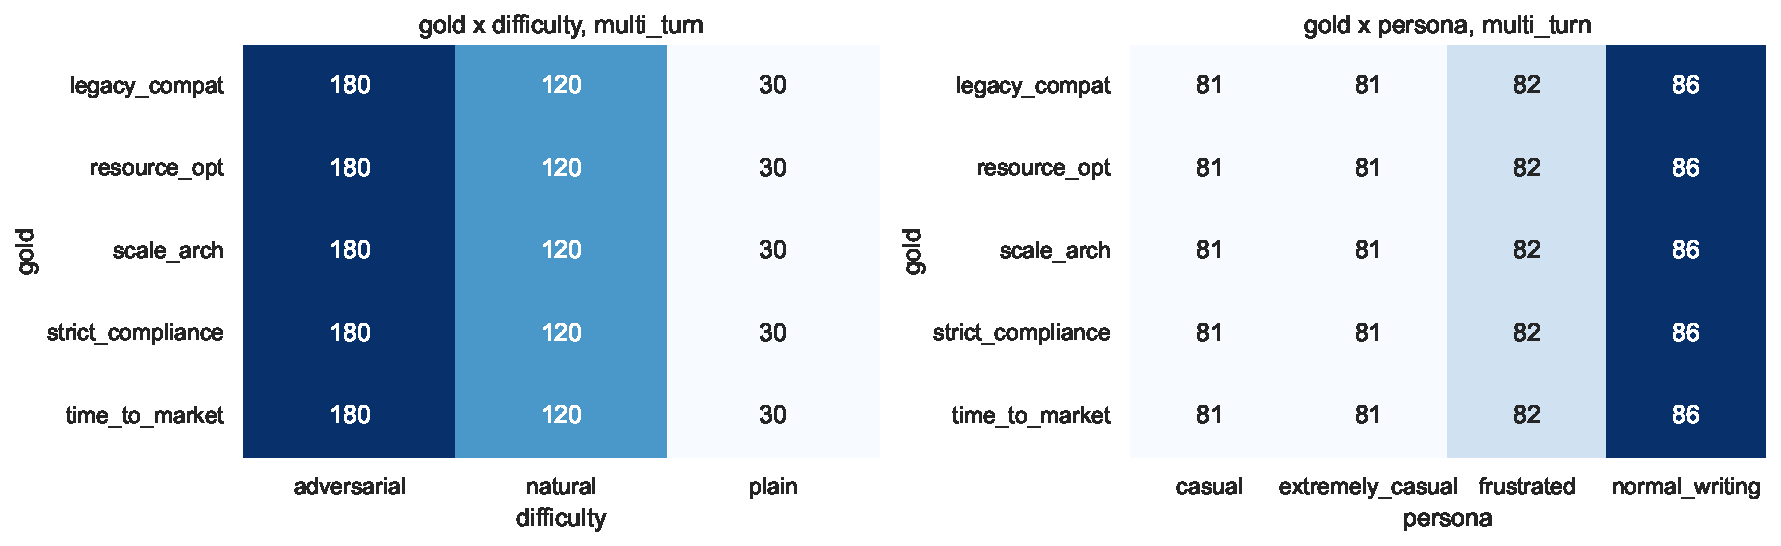
\includegraphics[width=\textwidth]{images/plots/anova/dataset_composition_multi_turn.pdf}
    \caption[Sample counts per sub-agent by tier and persona]{Sample counts per sub-agent, against difficulty tier and persona, single-turn (top) and multi-turn (bottom).}
    \label{fig:sample-balance}
\end{figure}

Figure~\ref{fig:sample-balance} cross-tabulates the correct sub-agent (\texttt{gold}) against the difficulty tier and against the persona, for the single-turn and the multi-turn dataset. Every sub-agent receives the same number of samples at every difficulty tier. Persona counts are near-equal but not identical across sub-agents, for example 81, 81, 82, and 86 samples for the four personas of a given sub-agent, because the deterministic shuffle in Section~\ref{subsec:pipeline-plan} distributes personas evenly only up to the remainder left when the sample count for a sub-agent is not a multiple of four. This gap, at most 5 samples out of about 330 per sub-agent, is negligible and does not compromise the balance that the tests in this section rely on.

\subsection{Extracted Features}
\label{subsec:surface-features}

The ANOVA in this section asks whether the correct sub-agent, \texttt{gold}, leaves a mark on the surface style of the request text, independent of its content. Section~\ref{sec:statistical-validation} requires the five sub-agents to be balanced in style: without that balance, a text-only classifier could route a request by a stylistic cue instead of by what the request asks. For each surface feature tested, the null hypothesis states that \texttt{gold} has no effect on it, that is, that the mean value of the feature is the same across the five sub-agent groups. Rejecting the null hypothesis for a feature means the sub-agent groups differ on that stylistic property.

For the ANOVA analysis, thirteen surface features are extracted from the text of each request. They are listed in Table~\ref{tab:surface-features}.

\begin{table}[H]
    \centering
    \begin{tabularx}{\textwidth}{@{}l>{\raggedright\arraybackslash}X@{}}
        \toprule
        \textbf{Feature} & \textbf{Definition} \\
        \midrule
        \texttt{n\_chars} & Number of characters \\
        \texttt{n\_words} & Number of words \\
        \texttt{n\_sentences} & Number of sentences \\
        \texttt{mean\_word\_len} & Mean word length, in characters \\
        \texttt{mean\_sent\_len} & Mean sentence length, in words \\
        \texttt{ttr} & Type-token ratio, distinct words divided by total words \\
        \texttt{pct\_upper} & Percentage of characters that are uppercase \\
        \texttt{pct\_digit} & Percentage of characters that are digits \\
        \texttt{n\_question} & Number of question marks \\
        \texttt{n\_comma} & Number of commas \\
        \texttt{long\_word\_ratio} & Percentage of words longer than seven characters \\
        \texttt{n\_units} & Count of unit and magnitude markers (\texttt{\%}, \texttt{\$}, MB, ms, req/s, and similar) \\
        \texttt{n\_number\_words} & Count of numbers written as words (\textit{eighty}, \textit{two weeks}, \textit{percent}) \\
        \bottomrule
    \end{tabularx}
    \caption[The thirteen surface features extracted from each request]{The thirteen surface features extracted from each request.}
    \label{tab:surface-features}
\end{table}

\subsection{One-Way ANOVA}
\label{subsec:anova-oneway}

For each of the thirteen surface features, a \emph{one-way ANOVA}, an ANOVA that tests one factor at a time, tests whether \texttt{gold} has an effect on that feature, for example whether the number of words in a request differs depending on which sub-agent is correct for it. Two quantities are reported for each test.

\paragraph{Effect size ($\omega^2$).} Omega squared is the percentage of the total variance in the feature explained by \texttt{gold}, corrected for the sampling noise that a simpler estimate (eta squared) would count as effect \citep{olejnikGeneralizedEtaOmega2003}. Cohen defines conventional thresholds for eta squared at 0.01 as small, 0.06 as medium, and 0.14 as large \citep{cohenStatisticalPowerAnalysis2013}; these thresholds are reused for omega squared as well.

\paragraph{Corrected significance ($p_{\text{holm}}$).} A one-way ANOVA returns a $p$-value for the null hypothesis that \texttt{gold} has no effect on a given feature. A raw $p$-value below 0.05 would count that effect as significant on its own. But thirteen tests are run at once, one per feature, and some of them are expected to fall below 0.05 purely by chance, even if \texttt{gold} has no real effect on any feature. The Holm method \citep{holmSimpleSequentiallyRejective1979} corrects for this. It raises the threshold each test must clear as more tests are run, and the corrected $p$-value is reported as $p_{\text{holm}}$. An effect counts as significant only when $p_{\text{holm}}$ stays below 0.05.

\bigskip

\begin{table}[htbp]
    \centering
    \small
    \begin{tabular}{@{}lrrrr@{}}
        \toprule
        & \multicolumn{2}{c}{\textbf{Single-turn}} & \multicolumn{2}{c}{\textbf{Multi-turn}} \\
        \textbf{Feature} & $\omega^2$ & $p_{\text{holm}}$ & $\omega^2$ & $p_{\text{holm}}$ \\
        \midrule
        \texttt{pct\_digit}        & \cellcolor{omegaMedium}0.132 & \textbf{$<$0.001} & \cellcolor{omegaMedium}0.082 & \textbf{$<$0.001} \\
        \texttt{n\_units}          & \cellcolor{omegaMedium}0.119 & \textbf{$<$0.001} & \cellcolor{omegaMedium}0.090 & \textbf{$<$0.001} \\
        \texttt{mean\_word\_len}   & \cellcolor{omegaMedium}0.063 & \textbf{$<$0.001} & \cellcolor{omegaMedium}0.075 & \textbf{$<$0.001} \\
        \texttt{long\_word\_ratio} & \cellcolor{omegaMedium}0.062 & \textbf{$<$0.001} & \cellcolor{omegaSmall}0.046  & \textbf{$<$0.001} \\
        \texttt{n\_comma}          & \cellcolor{omegaSmall}0.036  & \textbf{$<$0.001} & \cellcolor{omegaSmall}0.016  & \textbf{$<$0.001} \\
        \texttt{n\_chars}          & \cellcolor{omegaSmall}0.024  & \textbf{$<$0.001} & \cellcolor{omegaSmall}0.015  & \textbf{$<$0.001} \\
        \texttt{n\_words}          & \cellcolor{omegaSmall}0.016  & \textbf{$<$0.001} & 0.006 & \textbf{0.038} \\
        \texttt{n\_number\_words}  & \cellcolor{omegaSmall}0.015  & \textbf{$<$0.001} & \cellcolor{omegaSmall}0.011  & \textbf{0.002} \\
        \texttt{ttr}               & \cellcolor{omegaSmall}0.014  & \textbf{$<$0.001} & \cellcolor{omegaSmall}0.011  & \textbf{0.002} \\
        \texttt{pct\_upper}        & \cellcolor{omegaSmall}0.013  & \textbf{$<$0.001} & 0.003 & 0.242 \\
        \texttt{mean\_sent\_len}   & 0.004 & 0.120 & -0.001 & 1.000 \\
        \texttt{n\_sentences}      & 0.001 & 0.374 & -0.001 & 1.000 \\
        \texttt{n\_question}       & -0.002 & 0.914 & -0.001 & 1.000 \\
        \bottomrule
    \end{tabular}
    \caption[Effect of \texttt{gold} on surface features, single-turn and multi-turn]{Effect of \texttt{gold} on the thirteen surface features, single-turn and multi-turn.}
    \label{tab:gold-omega2}
\end{table}

Table~\ref{tab:gold-omega2} reports the effect of \texttt{gold} on all thirteen features, ordered by $\omega^2$: cells are shaded by magnitude, \colorbox{omegaSmall}{small}, \colorbox{omegaMedium}{medium}, \colorbox{omegaLarge}{large}, and left unshaded when negligible, and $p_{\text{holm}}$ is bold where it rejects the null hypothesis. The largest effect of \texttt{gold} falls on the count of numeric magnitudes, \texttt{pct\_digit} and \texttt{n\_units} at 0.132 and 0.119 in single-turn, 0.082 and 0.090 in multi-turn. When the correct sub-agent is \texttt{resource\_opt}, the request is more likely to state memory ceilings, cost budgets, or latency figures. Figure~\ref{fig:gold-effect} shows this difference directly, plotting the group means of \texttt{pct\_digit} and \texttt{n\_units} with a 95\% confidence interval per sub-agent, single-turn (top) and multi-turn (bottom).

\begin{figure}[htbp]
    \centering
    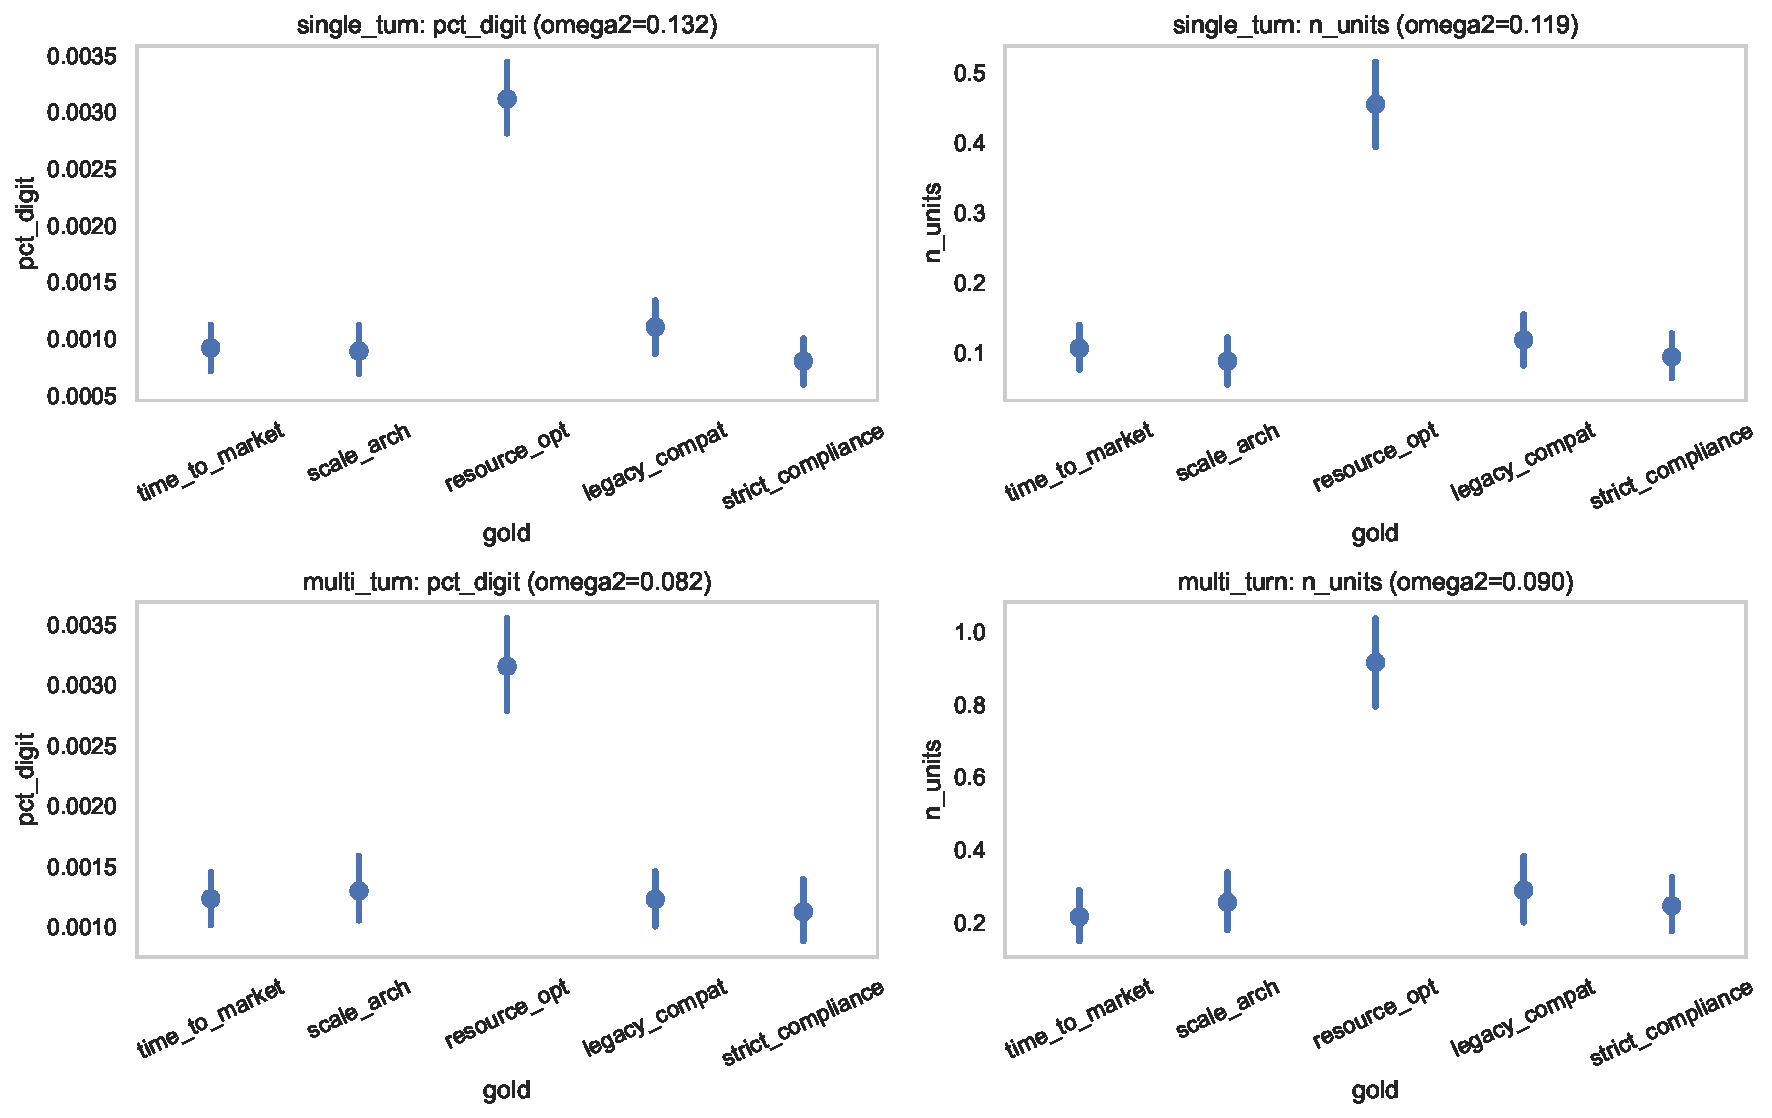
\includegraphics[width=\textwidth]{images/plots/anova/dataset_gold.pdf}
    \caption[Group means of \texttt{pct\_digit} and \texttt{n\_units} by \texttt{gold}]{Group means of \texttt{pct\_digit} and \texttt{n\_units} by \texttt{gold}, single-turn (top) and multi-turn (bottom).}
    \label{fig:gold-effect}
\end{figure}

\subsection{Levene's Test and the Kruskal-Wallis Test}
\label{subsubsec:levene-kruskal}

The one-way ANOVA in Section~\ref{subsec:anova-oneway} is valid only if the five \texttt{gold} groups share the same variance. If this assumption fails for a feature, the ANOVA's $p$-value for that feature cannot be trusted, and the effect it reports could be a product of unequal variance rather than a real difference between the groups. Two additional tests check this assumption and its consequences:

\begin{itemize}
    \item \textbf{Levene}'s test checks directly whether the five groups have equal variance, the assumption the ANOVA needs \citep{montgomeryDesignAnalysisExperiments2022}.
    \item The \textbf{Kruskal-Wallis} test \citep{montgomeryDesignAnalysisExperiments2022} compares the same \texttt{gold} groups on the ranks of the values instead of the raw values. This comparison needs no assumption about variance, so it stays valid even on a feature where Levene shows the ANOVA's assumption fails, and its verdict serves as a check on the ANOVA's own verdict for that feature.
\end{itemize}

Table~\ref{tab:levene-kruskal} reports both tests on the same thirteen features and the same \texttt{gold} factor as Table~\ref{tab:gold-omega2}, with both $p$-values corrected with Holm across that same family of thirteen tests. Bold marks a $p_{\text{holm}}$ below 0.05, rejecting the test's null hypothesis.

\begin{table}[htbp]
    \centering
    \small
    \begin{tabular}{@{}lrrrr@{}}
        \toprule
        & \multicolumn{2}{c}{\textbf{Single-turn}} & \multicolumn{2}{c}{\textbf{Multi-turn}} \\
        \textbf{Feature} & \textbf{Levene} $p_{\text{holm}}$ & \textbf{Kruskal} $p_{\text{holm}}$ & \textbf{Levene} $p_{\text{holm}}$ & \textbf{Kruskal} $p_{\text{holm}}$ \\
        \midrule
        \texttt{pct\_digit}        & \textbf{$<$0.001} & \textbf{$<$0.001} & \textbf{$<$0.001} & \textbf{$<$0.001} \\
        \texttt{n\_units}          & \textbf{$<$0.001} & \textbf{$<$0.001} & \textbf{$<$0.001} & \textbf{$<$0.001} \\
        \texttt{mean\_word\_len}   & 1.000          & \textbf{$<$0.001} & 1.000          & \textbf{$<$0.001} \\
        \texttt{long\_word\_ratio} & 0.654          & \textbf{$<$0.001} & 1.000          & \textbf{$<$0.001} \\
        \texttt{n\_comma}          & \textbf{0.002} & \textbf{$<$0.001} & 1.000          & \textbf{$<$0.001} \\
        \texttt{n\_chars}          & \textbf{0.009} & \textbf{$<$0.001} & 1.000          & \textbf{$<$0.001} \\
        \texttt{n\_words}          & \textbf{0.048} & \textbf{0.002} & 1.000          & \textbf{0.034} \\
        \texttt{n\_number\_words}  & 0.364          & \textbf{$<$0.001} & 0.555          & \textbf{0.001} \\
        \texttt{ttr}               & 0.504          & \textbf{$<$0.001} & 1.000          & \textbf{0.001} \\
        \texttt{pct\_upper}        & \textbf{$<$0.001} & \textbf{0.004} & \textbf{$<$0.001} & 0.282          \\
        \texttt{mean\_sent\_len}   & 1.000          & \textbf{0.047} & 1.000          & 1.000          \\
        \texttt{n\_sentences}      & 0.271          & 0.426          & 1.000          & 1.000          \\
        \texttt{n\_question}       & 1.000          & 0.929          & 1.000          & 1.000          \\
        \bottomrule
    \end{tabular}
    \caption[Levene and Kruskal-Wallis tests on \texttt{gold}, single-turn and multi-turn]{Levene's test and the Kruskal-Wallis test on the \texttt{gold} factor, single-turn and multi-turn.}
    \label{tab:levene-kruskal}
\end{table}

\textbf{Levene}'s test rejects equal variance on six features in the single-turn dataset (\texttt{pct\_digit}, \texttt{n\_units}, \texttt{n\_comma}, \texttt{n\_chars}, \texttt{n\_words}, \texttt{pct\_upper}) and three in the multi-turn dataset (\texttt{pct\_digit}, \texttt{n\_units}, \texttt{pct\_upper}). The ANOVA's equal-variance assumption therefore does not hold for these features.

The \textbf{Kruskal-Wallis} test reaches the same verdict as the ANOVA on twelve of the thirteen features in the single-turn dataset and on all thirteen in the multi-turn dataset. The one exception is \texttt{mean\_sent\_len} in single-turn: the ANOVA does not reject its null hypothesis ($p_{\text{holm}} = 0.120$), but the Kruskal-Wallis test does ($p_{\text{holm}} = 0.047$). This feature has the smallest effect size in Table~\ref{tab:gold-omega2} ($\omega^2 = 0.004$), and both raw $p$-values are close to 0.05 before correction ($p = 0.040$ for the ANOVA, $p = 0.016$ for Kruskal-Wallis). After Holm's correction, one is above 0.05 and the other is below it. Levene's test does not reject equal variance for this feature ($p_{\text{holm}} = 1.000$), so the disagreement is not caused by a violated assumption.

Levene's test shows that the ANOVA's equal-variance assumption fails for a minority of features, six in single-turn and three in multi-turn. Despite this, the Kruskal-Wallis test agrees with the ANOVA on every feature but one, even though it needs no such assumption. The $\omega^2$ values in Table~\ref{tab:gold-omega2} therefore describe a property of the data, not an artifact of the ANOVA's violated assumption.

\subsection{Games-Howell Test}
\label{subsec:anova-posthoc}

The one-way ANOVA does not identify which pairs of sub-agents differ on a feature. To test this, a Games-Howell test is performed on every feature whose one-way \texttt{gold} effect stays significant after the Holm correction and reaches an $\omega^2$ of at least 0.01, the conventional threshold for a small effect.

The Games-Howell test compares every pair of sub-agents on a feature, all ten pairs at once, and holds the probability of at least one false positive among them at 0.05. Unlike Tukey's HSD test \citep{montgomeryDesignAnalysisExperiments2022}, it does not assume equal variances across groups \citep{gamesPairwiseMultipleComparison1976}, so it applies directly to the features where Section~\ref{subsubsec:levene-kruskal} shows this assumption fails.
After the Games-Howell test, the $p$-values from all pairwise comparisons are corrected with Holm across the restricted family of features.

Figure~\ref{fig:posthoc} shows the pairwise mean differences for the four features with the largest \texttt{gold} effect. A blank cell marks a pair that is not significant after the Holm correction.

\begin{figure}[htbp]
    \centering
    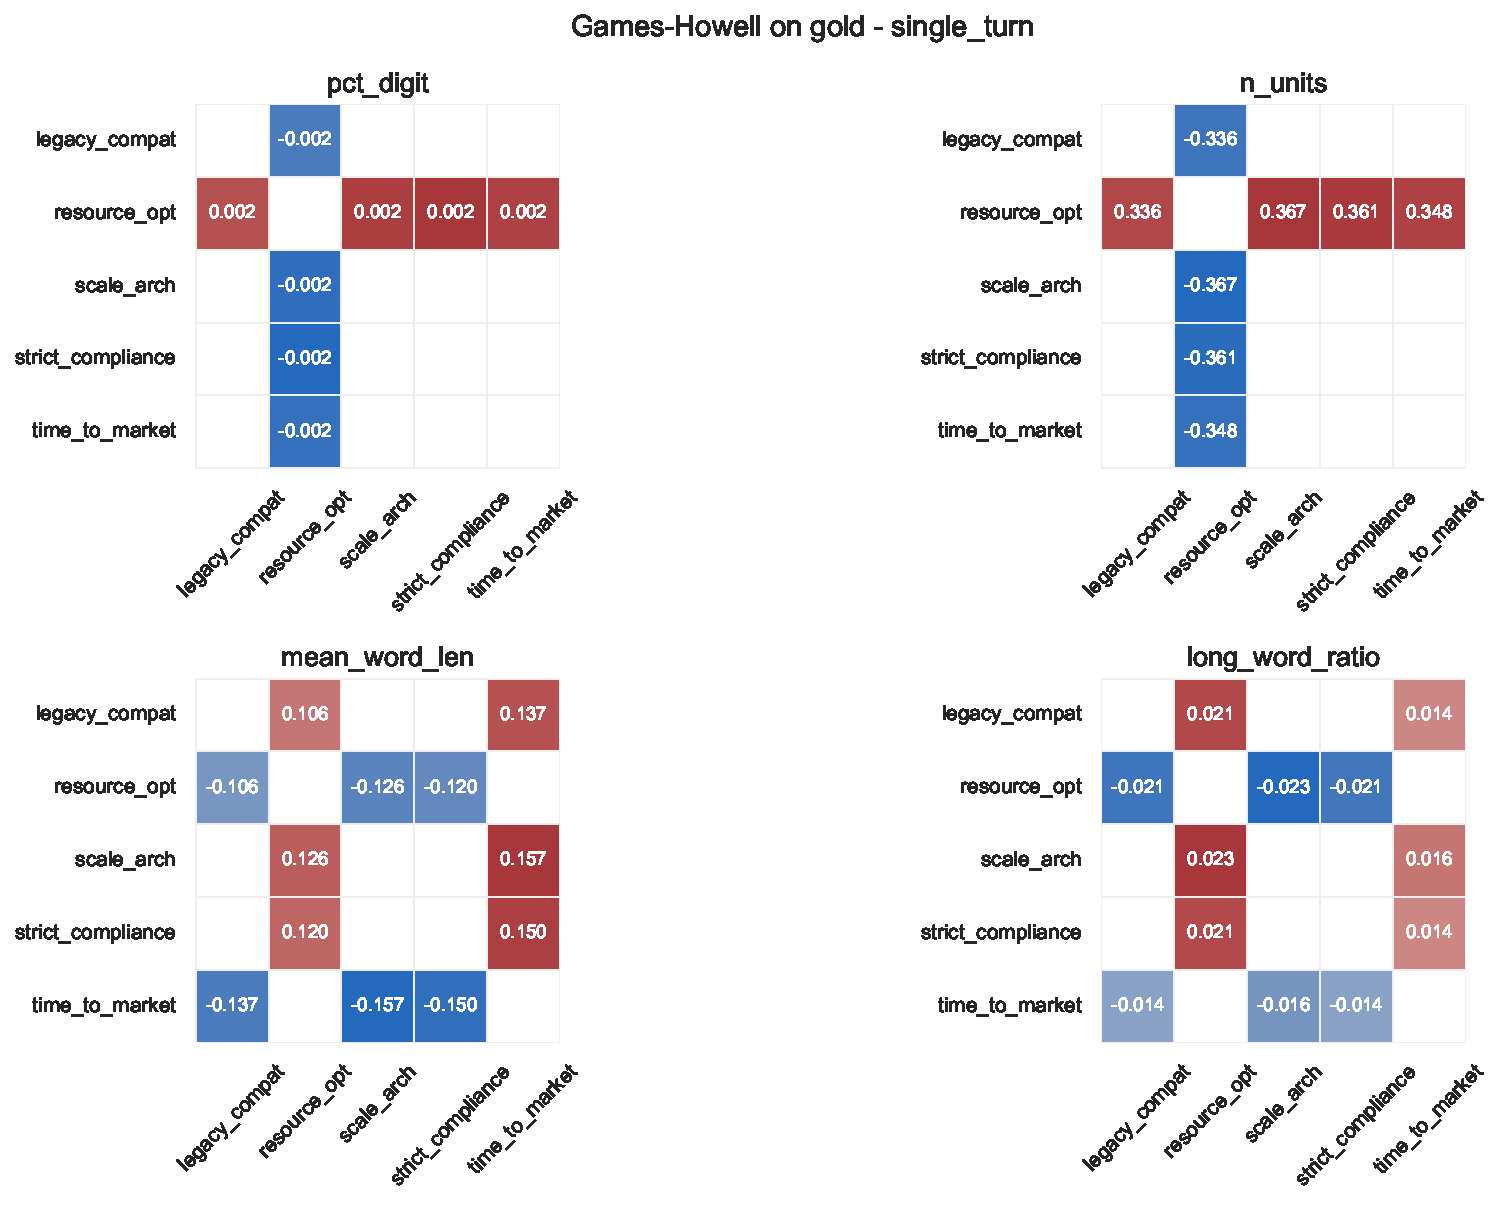
\includegraphics[width=\textwidth,height=0.46\textheight,keepaspectratio]{images/plots/anova/dataset_posthoc_single_turn.pdf}
    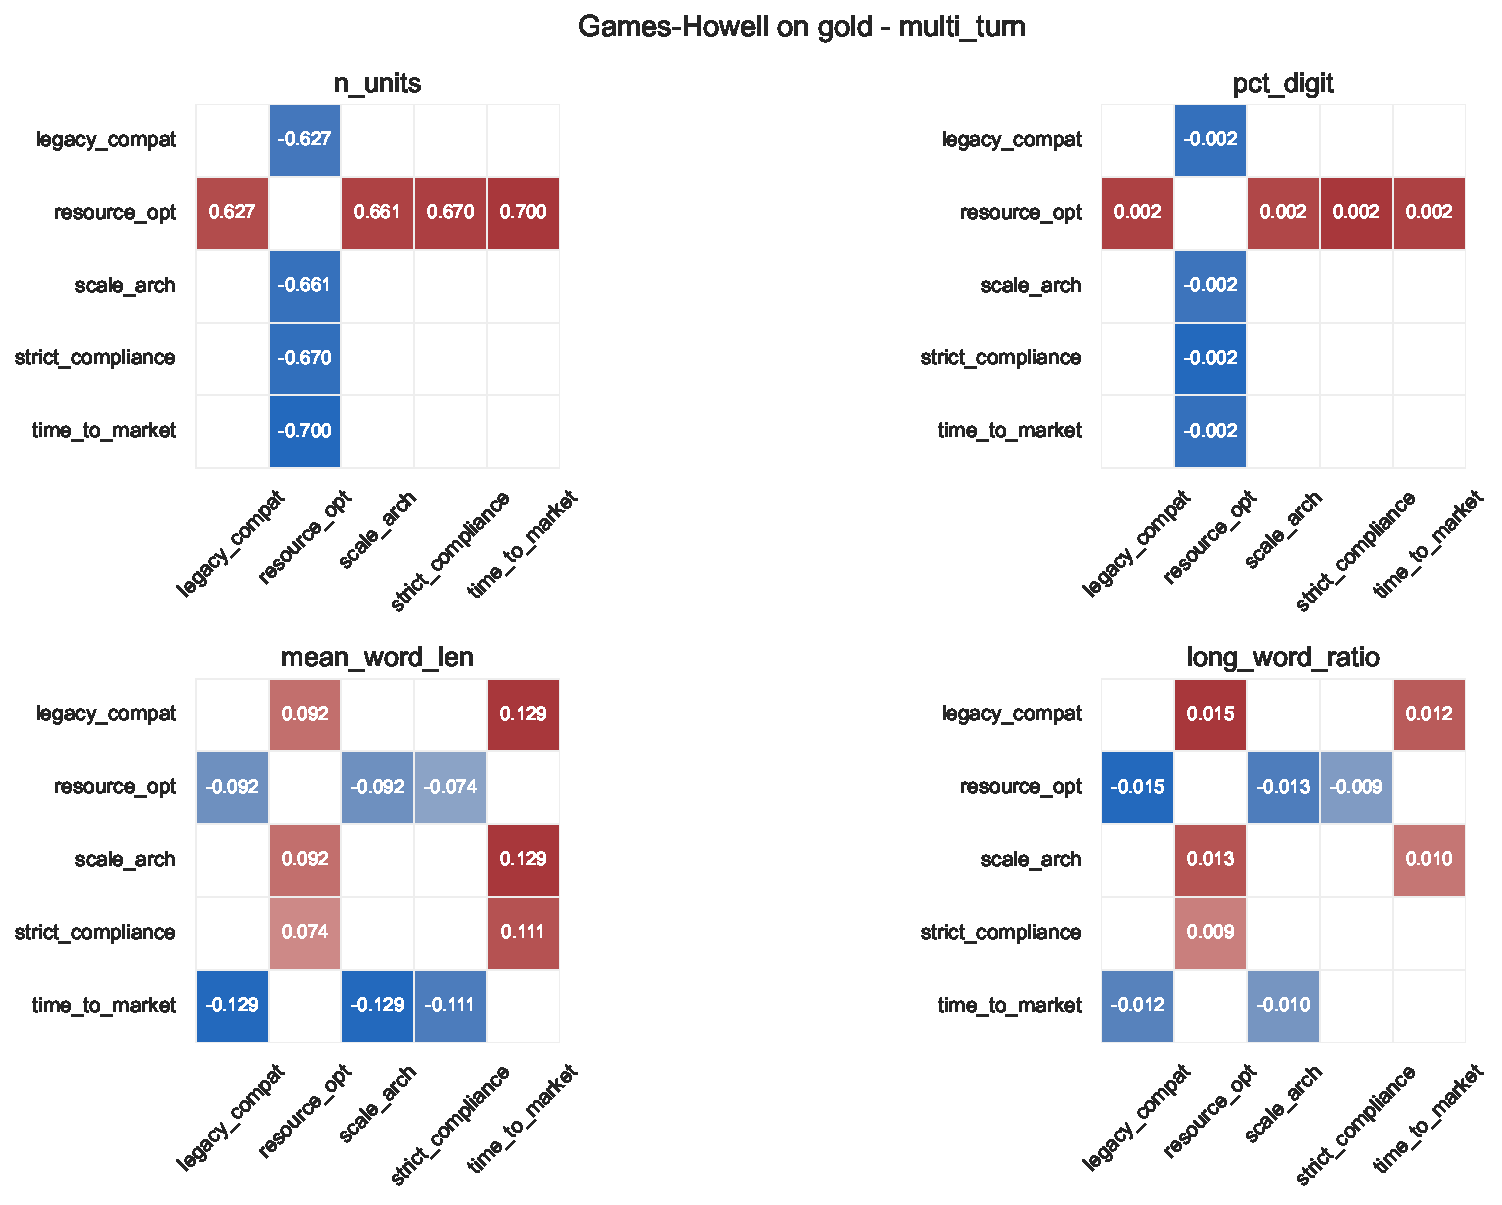
\includegraphics[width=\textwidth,height=0.46\textheight,keepaspectratio]{images/plots/anova/dataset_posthoc_multi_turn.pdf}
    \caption[Games-Howell pairwise comparisons on \texttt{gold} by dataset]{Games-Howell pairwise comparisons on \texttt{gold}, for the four surface features with the largest one-way effect, single-turn (top) and multi-turn (bottom) dataset. A blank cell means the pair is not significant after the Holm correction.}
    \label{fig:posthoc}
\end{figure}

The results on the single-turn dataset show the following structure:
\begin{itemize}
    \item On \texttt{pct\_digit} and \texttt{n\_units}, \texttt{resource\_opt} differs significantly from each of the other four sub-agents. None of the six pairs among those other four is significant. These two features therefore separate \texttt{resource\_opt} from the rest, but do not separate the remaining four sub-agents from each other.
    \item On \texttt{mean\_word\_len} and \texttt{long\_word\_ratio}, the sub-agents split into two blocks: \texttt{time\_to\_market} and \texttt{resource\_opt} on one side, \texttt{scale\_arch}, \texttt{legacy\_compat}, and \texttt{strict\_compliance} on the other. Every pair across the two blocks is significant, and no pair inside either block is. This split reflects domain-specific vocabulary: terms such as \textit{compliance}, \textit{infrastructure}, and \textit{migration} run longer than terms such as \textit{ship}, \textit{weeks}, and \textit{quick}.
\end{itemize}

The results on the multi-turn dataset show the same structure, with one exception:
\begin{itemize}
    \item On \texttt{pct\_digit} and \texttt{n\_units}, \texttt{resource\_opt} again differs significantly from each of the other four sub-agents, with no significant pair among those four.
    \item On \texttt{mean\_word\_len}, the same two blocks reappear: every pair across the two blocks is significant, and no pair inside either block is. On \texttt{long\_word\_ratio}, the same holds for five of the six pairs across the two blocks. The sixth pair, \texttt{time\_to\_market} against \texttt{strict\_compliance}, is not significant, even though the two sub-agents fall on opposite blocks.
\end{itemize}

This test confirms the same distinction among the five sub-agents. On \texttt{pct\_digit} and \texttt{n\_units}, \texttt{resource\_opt} separates from the other four. On \texttt{mean\_word\_len} and \texttt{long\_word\_ratio}, the five sub-agents split into two vocabulary blocks.

The stylistic imbalance that the one-way ANOVA detects is therefore not spread evenly across the five sub-agents. It traces to two distinct sources: \texttt{resource\_opt} stated apart from the other four by its numeric magnitude markers, and a two-block split in word length that follows domain vocabulary rather than the five sub-agents individually. Neither source separates all five sub-agents from each other on any single feature.

\subsection{Multiway ANOVA}
\label{subsec:anova-multiway}

The one-way test in Section~\ref{subsec:anova-oneway} examines one factor at a time. A \emph{multiway ANOVA} tests several factors together, so that the effect of each factor is estimated while holding the others fixed, and can also test whether two factors interact, that is, whether the effect of one factor changes depending on the level of the other. If, for example, \texttt{resource\_opt} requests used longer words only when the decoy was \texttt{time\_to\_market}, and shorter words only when the decoy was \texttt{scale\_arch}, averaging over decoys would hide the effect entirely.

Each interaction effect is isolated by comparing two nested regressions: a \texttt{full} model containing every combination of the listed factors, and a \texttt{reduced} model containing the same factors without any combination involving \texttt{gold}. The variance that the full model explains beyond the reduced model is the variance attributable to \texttt{gold}'s interactions with the other factors in that model. This gain is reported as \textbf{partial omega squared} ($\omega_p^2$): the gain divided by the variance that the reduced model left unexplained. It is corrected the same way as the one-way $\omega^2$, but for the sampling noise of the extra columns that the full model adds, on the block of interaction terms rather than on a single term \citep{olejnikGeneralizedEtaOmega2003}. Each comparison is tested with an F-test between the two nested models, Holm-corrected across the 13 features of each model.

\raggedbottom

Three such model pairs test for interactions between \texttt{gold} and the other design factors.

\begin{itemize}
    \item \textbf{Model 1 (style):} \texttt{gold * difficulty * persona}, fit on all 1650 samples.
    \item \textbf{Model 2 (difficulty):} \texttt{gold * decoy * difficulty}, fit on the 1500 samples that carry a decoy.
    \item \textbf{Model 3 (pattern):} \texttt{gold * pattern}, fit on the 900 \texttt{adversarial} samples.
\end{itemize}

Tables~\ref{tab:interactions-single} and~\ref{tab:interactions-multi} report partial $\omega^2$ and $p_{\text{holm}}$ for every feature and every model, single-turn and multi-turn. As in Table~\ref{tab:gold-omega2}, cells are shaded by magnitude, \colorbox{omegaSmall}{small}, \colorbox{omegaMedium}{medium}, \colorbox{omegaLarge}{large}, and left unshaded when negligible, using the same 0.01/0.06/0.14 thresholds \citep{cohenStatisticalPowerAnalysis2013}, and $p_{\text{holm}}$ is bold where it rejects the null hypothesis. These thresholds were defined for the one-way case, and applying them to partial omega squared can overstate the effect \citep{olejnikGeneralizedEtaOmega2003}.

Across the 78 tests spanning the three models and both datasets, only two cells reject the null hypothesis after Holm in single-turn and three in multi-turn. Their partial $\omega^2$ stays between 0.018 and 0.030 in every case, close to the small-effect threshold rather than far above it, so the conclusion holds even if the thresholds overstate the effect as described above.

The multiway analysis therefore finds no interaction effect worth reporting beyond the one-way ANOVA in Section~\ref{subsec:anova-oneway}.

\begin{table}[H]
    \centering
    \small
    \begin{tabular}{@{}lrrrrrr@{}}
        \toprule
        & \multicolumn{2}{c}{\textbf{Model 1 (style)}} & \multicolumn{2}{c}{\textbf{Model 2 (difficulty)}} & \multicolumn{2}{c}{\textbf{Model 3 (pattern)}} \\
        \textbf{Feature} & $\omega_p^2$ & $p_{\text{holm}}$ & $\omega_p^2$ & $p_{\text{holm}}$ & $\omega_p^2$ & $p_{\text{holm}}$ \\
        \midrule
        \texttt{pct\_digit}        & -0.008 & 1.000 & -0.004 & 1.000 & -0.007 & 1.000 \\
        \texttt{n\_units}          & -0.000 & 1.000 & -0.005 & 1.000 & -0.010 & 1.000 \\
        \texttt{mean\_word\_len}   & -0.005 & 1.000 & -0.005 & 1.000 & -0.005 & 1.000 \\
        \texttt{long\_word\_ratio} & -0.003 & 1.000 & -0.008 & 1.000 & -0.003 & 1.000 \\
        \texttt{n\_comma}          & -0.002 & 1.000 & 0.004  & 1.000 & -0.002 & 1.000 \\
        \texttt{n\_chars}          & -0.001 & 1.000 & -0.000 & 1.000 & -0.000 & 1.000 \\
        \texttt{n\_words}          & -0.001 & 1.000 & 0.001  & 1.000 & -0.001 & 1.000 \\
        \texttt{n\_number\_words}  & -0.006 & 1.000 & -0.004 & 1.000 & 0.003  & 1.000 \\
        \texttt{ttr}               & 0.005  & 1.000 & -0.003 & 1.000 & 0.003  & 1.000 \\
        \texttt{pct\_upper}        & \cellcolor{omegaSmall}0.022  & \textbf{0.009} & -0.011 & 1.000 & -0.004 & 1.000 \\
        \texttt{mean\_sent\_len}   & -0.006 & 1.000 & 0.008  & 0.855 & -0.004 & 1.000 \\
        \texttt{n\_sentences}      & 0.011  & 0.490 & \cellcolor{omegaSmall}0.020  & \textbf{0.007} & 0.009  & 0.808 \\
        \texttt{n\_question}       & 0.009  & 0.867 & 0.006  & 1.000 & -0.006 & 1.000 \\
        \bottomrule
    \end{tabular}
    \caption[Partial $\omega^2$ of \texttt{gold} interaction terms, single-turn dataset]{Partial $\omega^2$ ($\omega_p^2$) of the \texttt{gold} interaction terms, single-turn dataset.}
    \label{tab:interactions-single}

    \vspace{3em}

    \begin{tabular}{@{}lrrrrrr@{}}
        \toprule
        & \multicolumn{2}{c}{\textbf{Model 1 (style)}} & \multicolumn{2}{c}{\textbf{Model 2 (difficulty)}} & \multicolumn{2}{c}{\textbf{Model 3 (pattern)}} \\
        \textbf{Feature} & $\omega_p^2$ & $p_{\text{holm}}$ & $\omega_p^2$ & $p_{\text{holm}}$ & $\omega_p^2$ & $p_{\text{holm}}$ \\
        \midrule
        \texttt{pct\_digit}        & \cellcolor{omegaSmall}0.018  & \textbf{0.045} & -0.005 & 1.000 & -0.007 & 1.000 \\
        \texttt{n\_units}          & 0.004  & 0.975 & 0.002  & 1.000 & -0.004 & 1.000 \\
        \texttt{mean\_word\_len}   & 0.010  & 0.585 & 0.010  & 0.397 & -0.000 & 1.000 \\
        \texttt{long\_word\_ratio} & 0.001  & 0.975 & 0.001  & 1.000 & 0.003  & 1.000 \\
        \texttt{n\_comma}          & -0.000 & 0.975 & 0.002  & 1.000 & 0.004  & 1.000 \\
        \texttt{n\_chars}          & 0.006  & 0.975 & 0.006  & 1.000 & -0.003 & 1.000 \\
        \texttt{n\_words}          & 0.006  & 0.975 & 0.005  & 1.000 & -0.003 & 1.000 \\
        \texttt{n\_number\_words}  & 0.006  & 0.975 & 0.005  & 1.000 & 0.006  & 1.000 \\
        \texttt{ttr}               & 0.003  & 0.975 & -0.008 & 1.000 & -0.002 & 1.000 \\
        \texttt{pct\_upper}        & \cellcolor{omegaSmall}0.030  & \textbf{$<$0.001} & -0.004 & 1.000 & -0.006 & 1.000 \\
        \texttt{mean\_sent\_len}   & 0.008  & 0.786 & 0.003  & 1.000 & -0.004 & 1.000 \\
        \texttt{n\_sentences}      & 0.007  & 0.913 & 0.010  & 0.390 & -0.002 & 1.000 \\
        \texttt{n\_question}       & \cellcolor{omegaSmall}0.019  & \textbf{0.025} & -0.004 & 1.000 & -0.004 & 1.000 \\
        \bottomrule
    \end{tabular}
    \caption[Partial $\omega^2$ of \texttt{gold} interaction terms, multi-turn dataset]{Partial $\omega^2$ ($\omega_p^2$) of the \texttt{gold} interaction terms, multi-turn dataset.}
    \label{tab:interactions-multi}
\end{table}

\flushbottom

\subsection{Classifiers on Surface Features Alone}
\label{subsec:shortcut-classifiers}

The one-way and multiway ANOVA are univariate. Several small effects could still combine into one effect that a classifier exploits. A classifier that is trained on the thirteen surface features, with no access to the request text, measures the accuracy that such a combination reaches.

Two classifiers are trained, both on the same scenario-grouped 5-fold cross-validation and the same out-of-fold accuracy, broken down by difficulty tier, as the text-only classifiers of Section~\ref{sec:dataset-baselines}:

\begin{itemize}
    \item \textbf{Logistic regression}, trained five times to isolate the contribution of the numeric features to the accuracy reached from surface features alone:
    \begin{itemize}
        \item on all thirteen features, to establish the maximum accuracy attainable from surface features alone;
        \item on the feature set without \texttt{pct\_digit}, to measure how much the percentage of digit characters contributes to accuracy;
        \item on \texttt{pct\_digit} alone, to measure that feature's own contribution;
        \item on the feature set without the numeric features (\texttt{pct\_digit}, \texttt{n\_units}, \texttt{n\_number\_words}), to measure how much digit characters, unit markers, and numbers written as words together contribute to accuracy;
        \item on the numeric features alone, to measure how much they increase classification accuracy by themselves.
    \end{itemize}
    \item \textbf{Random forest}, trained once, on all thirteen features. It gives a second, non-linear ceiling, and it is the classifier used for the feature importance attribution of Section~\ref{subsec:feature-importance}.
\end{itemize}

Figures~\ref{fig:ceiling-single} and~\ref{fig:ceiling-multi} report accuracy for each of the six runs above, with chance accuracy marked for comparison.

\begin{figure}[htbp]
    \centering
    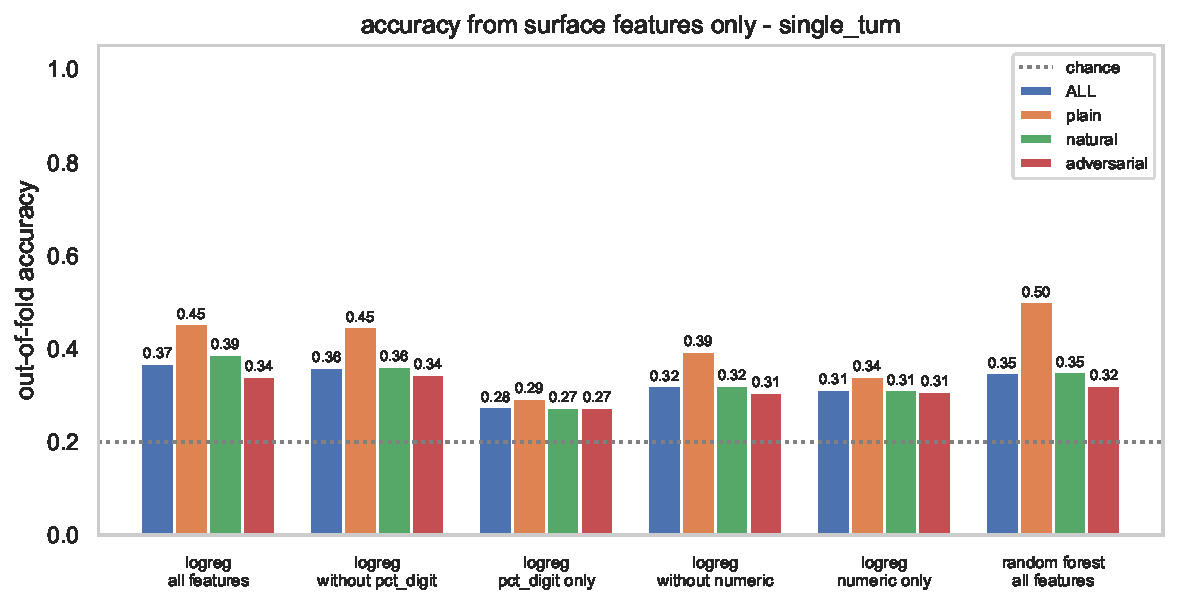
\includegraphics[width=\textwidth]{images/plots/anova/dataset_ceiling_single_turn.pdf}
    \caption[Accuracy from surface features alone, single-turn dataset]{Accuracy from surface features alone, single-turn dataset. The dotted line marks chance.}
    \label{fig:ceiling-single}
\end{figure}

\begin{figure}[htbp]
    \centering
    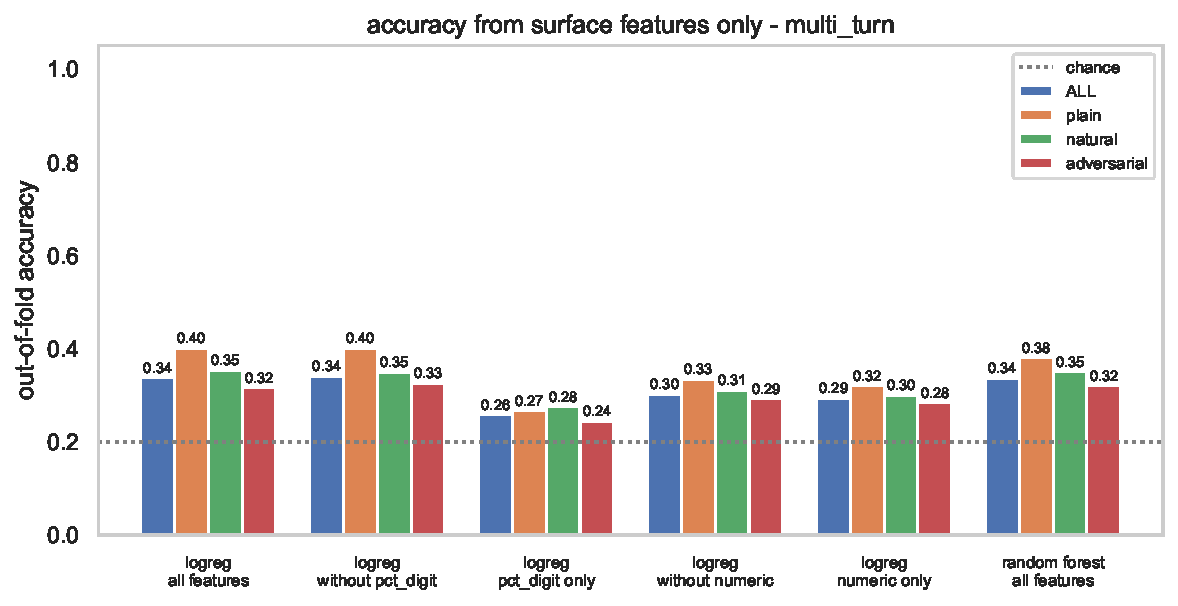
\includegraphics[width=\textwidth]{images/plots/anova/dataset_ceiling_multi_turn.pdf}
    \caption[Accuracy from surface features alone, multi-turn dataset]{Accuracy from surface features alone, multi-turn dataset. The dotted line marks chance.}
    \label{fig:ceiling-multi}
\end{figure}

Removing \texttt{pct\_digit} alone has a negligible effect on accuracy: 0.368 to 0.360 in single-turn and 0.337 to 0.341 in multi-turn. Removing all three numeric features instead costs a measurable amount of accuracy: from 0.368 to 0.320 in single-turn, and from 0.337 to 0.302 in multi-turn. The numeric features alone reach 0.313 in single-turn and 0.293 in multi-turn, nearly matching the 0.368 and 0.337 reached with all thirteen features. The other ten features therefore add only about 0.05 of accuracy beyond the numeric features. This shows that the effect of \texttt{gold} on surface features, reported in Section~\ref{subsec:anova-oneway}, is caused by the numeric features. Their accuracy alone, 0.313 and 0.293, is therefore the figure that measures the size of that effect.

Because the effect is spread across the numeric features rather than tied to \texttt{pct\_digit} alone, removing digits from the generation prompt is unlikely to lower accuracy. A magnitude such as \textit{500ms} can still be written as \textit{five hundred milliseconds}: the digit disappears, but \texttt{n\_units} or \texttt{n\_number\_words} would capture the same magnitude instead, so the information the classifier uses stays in the text. On both datasets and on every tier, the surface-only accuracy stays well below the bag-of-words baseline, 0.684 in single-turn and 0.645 in multi-turn overall, reported in Table~\ref{tab:text-baselines}. The higher accuracy that the bag-of-words classifier reaches from the request text is therefore not explained by these thirteen surface features alone.

\subsection{Feature Importance: SHAP}
\label{subsec:feature-importance}

Section~\ref{subsec:shortcut-classifiers} does not establish which of the thirteen surface features drive the accuracy of its classifiers, or which sub-agent each one favors.

\textbf{SHAP} (SHapley Additive exPlanations) \citep{lundbergUnifiedApproachInterpreting2017} assigns each feature, for a single prediction, a \emph{SHAP value}: how much that feature moved the prediction away from a baseline where no feature is known. The attribution used here, TreeSHAP \citep{lundbergExplainableAITrees2019}, requires a tree-based model, so it is computed on the random forest classifier of Section~\ref{subsec:shortcut-classifiers}, rather than on the logistic regression. Averaging the absolute SHAP value of a feature across samples ranks features by their overall contribution to the classifier. This classifier predicts one of five sub-agents, and SHAP is computed separately for each one, so a feature gets five SHAP values, one per sub-agent. A feature whose value is large for one sub-agent and small for the other four is important specifically for classifying that one sub-agent.

Figures~\ref{fig:shap-single} and~\ref{fig:shap-multi} report the mean absolute SHAP value per feature and per sub-agent, out of fold, for the seven features with the largest total, on the single-turn and the multi-turn dataset respectively.

\raggedbottom

\begin{figure}[H]
    \centering
    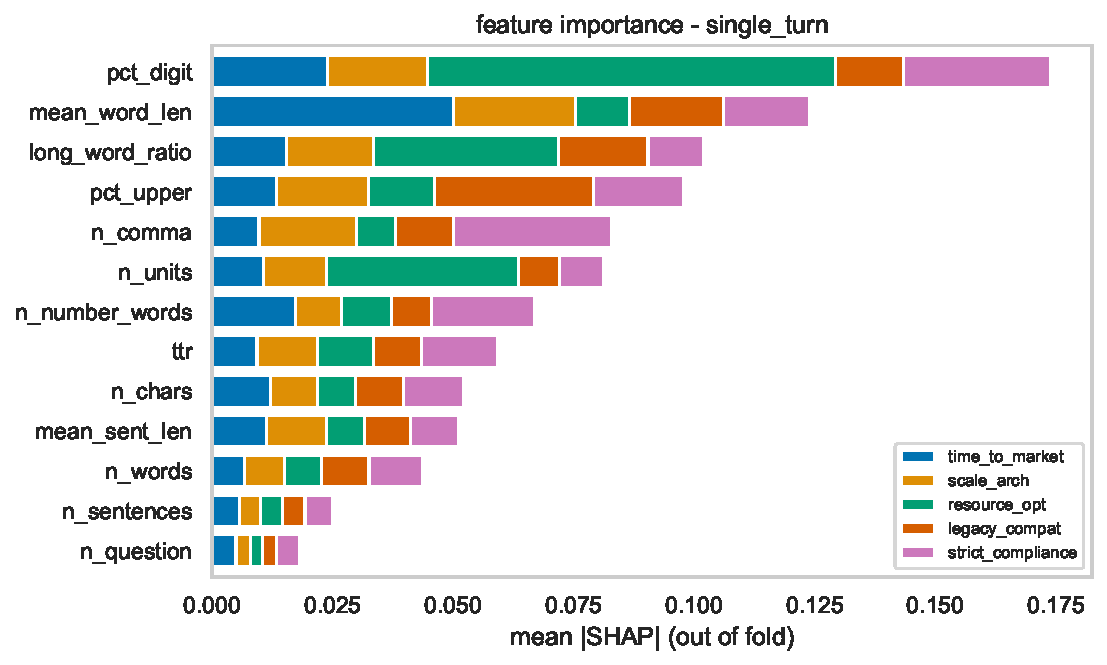
\includegraphics[width=0.9\textwidth]{images/plots/anova/dataset_shap_single_turn.pdf}
    \caption[Mean absolute SHAP value per feature and sub-agent, single-turn dataset]{Mean absolute SHAP value, out of fold, per feature and sub-agent, single-turn dataset.}
    \label{fig:shap-single}
\end{figure}

\begin{figure}[H]
    \centering
    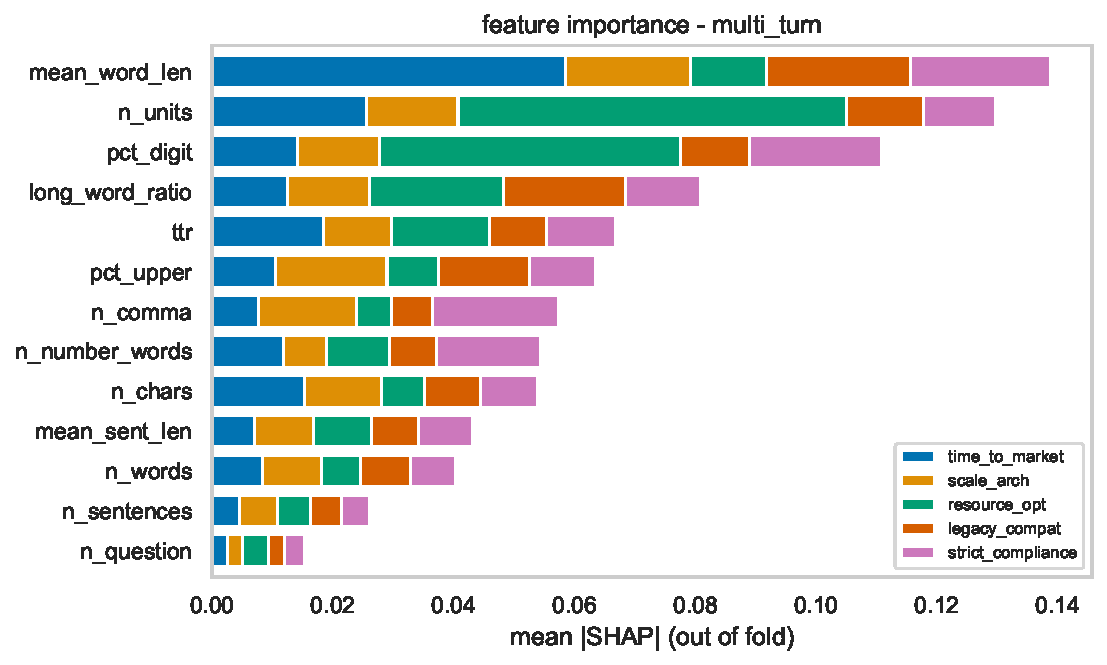
\includegraphics[width=0.9\textwidth]{images/plots/anova/dataset_shap_multi_turn.pdf}
    \caption[Mean absolute SHAP value per feature and sub-agent, multi-turn dataset]{Mean absolute SHAP value, out of fold, per feature and sub-agent, multi-turn dataset.}
    \label{fig:shap-multi}
\end{figure}

\flushbottom

Nearly half of the total SHAP attribution of \texttt{pct\_digit} concentrates on \texttt{resource\_opt} in single-turn (0.0847 of 0.174, 49\%), and the same holds for \texttt{n\_units} (49\% in both single-turn and multi-turn). This concentration is weaker for \texttt{pct\_digit} in multi-turn, at 45\%. No other feature concentrates this strongly on a single sub-agent. This confirms the Games-Howell test result of Section~\ref{subsec:anova-posthoc}. The remaining concentrations are weaker but consistent with the same test: \texttt{mean\_word\_len} concentrates on \texttt{time\_to\_market} (about 40\% in both datasets), and \texttt{n\_comma} concentrates on \texttt{strict\_compliance}.

\subsection{Summary}
\label{subsec:anova-summary}

The one-way ANOVA finds a medium effect of \texttt{gold} on only two of the thirteen surface features, \texttt{pct\_digit} and \texttt{n\_units}, both tied to numeric magnitudes in the request text. Every other feature reaches at most a small effect. The Games-Howell test and the SHAP attribution trace the effect on \texttt{pct\_digit} and \texttt{n\_units} to a single sub-agent: \texttt{resource\_opt} states memory ceilings, cost budgets, and latency figures more often than the other four sub-agents, and \texttt{pct\_digit} and \texttt{n\_units} do not separate those other four sub-agents from each other. The multiway ANOVA finds the \texttt{gold} effect on \texttt{pct\_digit} and \texttt{n\_units} independent of \texttt{difficulty}, \texttt{persona}, \texttt{decoy}, and \texttt{pattern}: almost all interaction tests fail to reject the null hypothesis.

Section~\ref{subsec:lexical-separability} requires the sub-agents to be balanced in writing style, not only in vocabulary, and the analysis in this section shows this requirement is not met exactly: \texttt{pct\_digit}, \texttt{n\_units}, \texttt{mean\_word\_len}, and \texttt{long\_word\_ratio} all differ significantly across \texttt{gold}. The purpose of that requirement is to keep a text-only classifier from routing a request by a stylistic marker instead of by its content. A classifier trained on the thirteen surface features reaches its ceiling accuracy almost entirely from the numeric features alone, 0.313 in single-turn and 0.293 in multi-turn against 0.368 and 0.337 for the full feature set (Section~\ref{subsec:shortcut-classifiers}). Both figures stay well below the bag-of-words baseline of 0.684 and 0.645 (Table~\ref{tab:text-baselines}).

Since the thirteen surface features cannot reach that baseline, the accuracy of the bag-of-words classifier must come from the lexical content of the request, the word choices the surface features do not capture, rather than from its style. Besides the numeric features, only \texttt{mean\_word\_len} and \texttt{long\_word\_ratio} differ significantly across \texttt{gold}, and they add only about 0.05 of accuracy over the numeric features alone (Section~\ref{subsec:shortcut-classifiers}). This residual style imbalance is too small for a text-only classifier to route requests by style at a level that would compromise the purpose of the balance requirement in Section~\ref{subsec:lexical-separability}: keeping a request from being routed by how it is written instead of what it asks.



\chapter{Hidden-State Probing: Setup and Results}
\label{chap:probing-results}

Chapter~\ref{chap:dataset-construction} confirms that the single-turn and multi-turn datasets are suitable for a probing experiment.

This chapter describes the experimental setup and reports the results obtained on eight open-weight models. Section~\ref{sec:model-choice} describes the eight models first, since the routing task, the hidden-state capture, the layer sweep and the results of the later sections are all defined for each model. Section~\ref{sec:ch7-probing-setup} describes the coordinator's routing task, the hidden-state capture procedure, the layer sweep that trains one probe per layer to find the optimal layer, and the metrics used to compare the probe against the model. Section~\ref{sec:ch7-results} reports the results obtained for each model, on the single-turn and the multi-turn dataset. Section~\ref{sec:ch7-observations} summarizes what these results show, including whether the differences between probe and model are significant.


\section{Model Choice}
\label{sec:model-choice}

The experiment runs on eight open-weight models, chosen to satisfy the requirements of Section~\ref{subsec:model-pool-requirements}. The model pool spans:

\begin{itemize}
    \item the Gemma 4 family by Google DeepMind \cite{teamGemma4Technical2026}, at three parameter sizes: E2B (5B total parameters, of which 2.3B are effective due to its internal architecture \cite{teamGemma4Technical2026}), 12B, and 26B A4B (a mixture-of-experts model, as defined in Section~\ref{subsec:dense-moe}, with 26B total parameters, of which 3.8B are active per token \cite{teamGemma4Technical2026}). Gemma 4 is the latest model family that Google DeepMind had released as of this writing (September 2026)
    \item the Qwen3 family by the Qwen Team (Alibaba) \cite{yangQwen3TechnicalReport2025}, at two parameter sizes: 4B and 8B
    \item GPT-OSS 20B by OpenAI \cite{openaiGptoss120bGptoss20bModel2025}
    \item Llama 3.3 70B Instruct by Meta \cite{MetallamaLlama3370BInstructHugging2024}
    \item Qwen2.5 72B Instruct by the Qwen Team (Alibaba) \cite{qwenQwen25TechnicalReport2025}
\end{itemize}

The model pool allows the probe to be tested on models from different providers, whose parameter count spans from a few billion to over seventy billion. Table~\ref{tab:model-properties} reports the architecture, parameter count, and layer count of each model. Each model family also relies on its own chat template, which is needed to format the prompt and the tool definitions correctly and to read the response correctly, as described in Section~\ref{subsec:rendered-example}.

Every model is configured to generate with sampling disabled, under greedy decoding as described in Section~\ref{subsec:decoding}, so that its routing decision is deterministic. This setting satisfies the replicability requirement that Section~\ref{subsec:model-pool-requirements} states for the model pool.

\begin{table}[htbp]
    \centering
    \footnotesize
    \setlength{\tabcolsep}{4pt}
    \begin{tabular}{lllrrrrl}
        \toprule
        Full name & Identifier & Provider & Total & Active & Layers & $d_{\mathrm{model}}$ & Chat template \\
        \midrule
        Gemma 4 E2B IT & \texttt{gemma4-e2b-it} & Google DeepMind & 5B & 2.3B & 35 & 1536 & gemma4 \\
        Qwen3 4B Instruct 2507 & \texttt{qwen3-4b} & Qwen Team (Alibaba) & 4B & 4B & 36 & 2560 & hermes \\
        Qwen3 8B & \texttt{qwen3-8b} & Qwen Team (Alibaba) & 8B & 8B & 36 & 4096 & hermes \\
        Gemma 4 12B IT & \texttt{gemma4-12b-it} & Google DeepMind & 12B & 12B & 48 & 3840 & gemma4 \\
        GPT-OSS 20B & \texttt{gpt-oss-20b} & OpenAI & 20.9B & 3.6B & 24 & 2880 & harmony \\
        Gemma 4 26B A4B IT & \texttt{gemma4-26b-a4b-it} & Google DeepMind & 26B & 3.8B & 30 & 2816 & gemma4 \\
        Llama 3.3 70B Instruct & \texttt{llama3.3-70b} & Meta & 70B & 70B & 80 & 8192 & llama3 \\
        Qwen2.5 72B Instruct & \texttt{qwen2.5-72b} & Qwen Team (Alibaba) & 72B & 72B & 80 & 8192 & hermes \\
        \bottomrule
    \end{tabular}
    \caption[Properties of the eight models used in this chapter]{Properties of the eight models used in this chapter.}
    \label{tab:model-properties}
\end{table}

\subsection{Chain-of-Thought Output}
\label{subsec:ch7-reasoning-traces}

Section~\ref{subsec:chain-of-thought} describes chain-of-thought output as text that a model generates before its response. Both the Gemma 4 family and the Qwen3 family in this pool call this a \emph{thinking mode} and let it be turned on or off at inference time \cite{teamGemma4Technical2026, yangQwen3TechnicalReport2025}.

In this work, thinking mode is always turned off where available, so the models are compared under the same condition. The only exception is GPT-OSS 20B, which, by design, does not allow chain-of-thought output to be disabled \cite{openaiGptoss120bGptoss20bModel2025}. Instead, GPT-OSS 20B exposes a \emph{reasoning effort} setting, with three levels (\texttt{low}, \texttt{medium}, \texttt{high}), that controls how long this chain-of-thought output is \cite{openaiGptoss120bGptoss20bModel2025}. In this work, the reasoning effort is set to \texttt{low}.


\section{Probing Setup and Routing Task}
\label{sec:ch7-probing-setup}

\subsection{Coordinator Setup}
\label{subsec:ch7-coordinator-prompt}

Each model in the pool of Section~\ref{sec:model-choice} is used as the coordinator of the centralized topology described in Section~\ref{subsec:topology-centralized}: a single supervisor that reads one request, single-turn or multi-turn, and routes it to one of the five sub-agents from Section~\ref{subsec:sub-agent-taxonomy}. A system prompt instructs the model on its coordinator role and the routing task that it has to perform, and lists the collision graph of Section~\ref{subsec:collision-graph}. The prompt is shared by all eight models and reported in Appendix~\ref{sec:appendix-coordinator-prompt}.

The coordinator states its routing decision through the function-calling interface described in Section~\ref{sec:structured-output}. Each sub-agent is declared to the model as a tool, and the coordinator routes a request by calling the tool representing the chosen sub-agent exactly once. Each tool's description states the sub-agent's role, the type of concerns that it handles, and an example request that routes to it. Each tool requires no argument from the coordinator. The five tool definitions are reported in Appendix~\ref{sec:appendix-subagent-tools}. The tool declarations are rendered into the prompt alongside the system prompt by the model's own chat template, the same mechanism that Section~\ref{subsec:rendered-example} describes for formatting a prompt and its tool definitions. The model's prediction is therefore obtained by reading which one of the available tools the model invokes.

None of the five sub-agents is implemented: the experiment only records which tool the coordinator invokes.

\subsection{Hidden-State Capture and the Model's Prediction}
\label{subsec:ch7-hook}

For every request, the same run of the model is used to obtain both the hidden states and the tool call that defines the model's own routing decision. This capture follows the fixed sequence of steps shown in Figure~\ref{fig:hook-sequence}.

\begin{figure}[ht]
	\centering
	\vspace{4mm}
	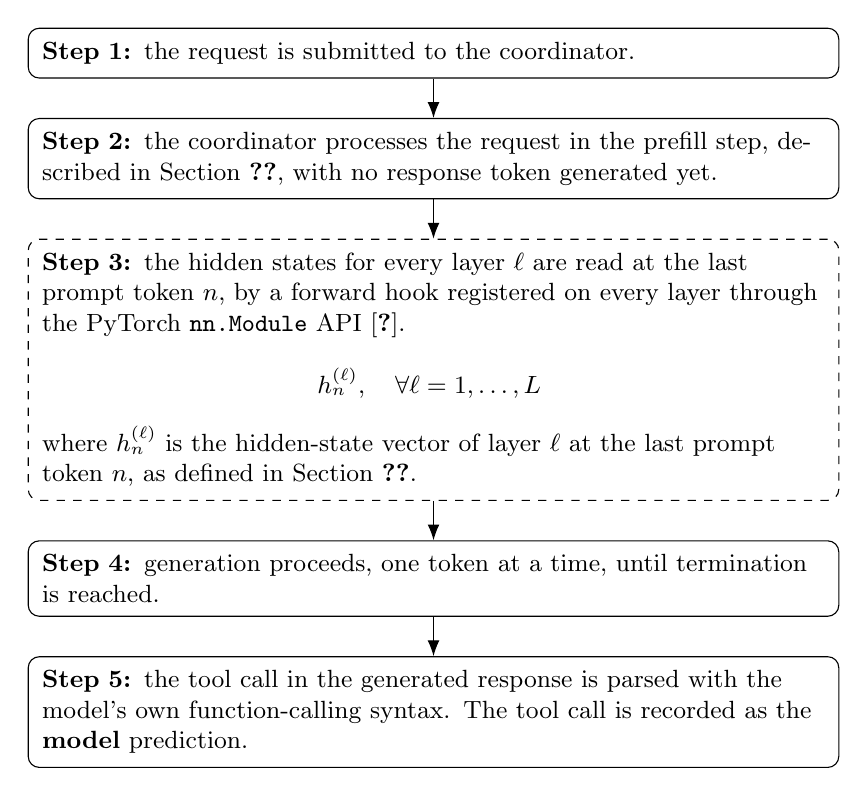
\begin{tikzpicture}[
		node distance=5mm,
		every node/.style={font=\small},
		seqstep/.style={draw, rounded corners, align=left, text width=0.82\textwidth, inner sep=5pt},
		seqcapture/.style={draw, dashed, rounded corners, align=left, text width=0.82\textwidth, inner sep=5pt},
		arr/.style={-{Latex[length=2mm]}}
		]
		\node[seqstep] (s1) {\textbf{Step 1:} the request is submitted to the coordinator.};
		\node[seqstep, below=of s1] (s2) {\textbf{Step 2:} the coordinator processes the request in the prefill step, described in Section~\ref{subsec:prefill-decode}, with no response token generated yet.};
		\node[seqcapture, below=of s2] (s3) {%
			\begin{minipage}{\linewidth}
				\textbf{Step 3:} the hidden states for every layer $\ell$ are read at the last prompt token $n$, by a forward hook registered on every layer through the PyTorch \texttt{nn.Module} API \cite{ModulePyTorch214}.
				\begin{center}
					\vspace{2pt}
					$h^{(\ell)}_n, \quad \forall \ell = 1, \dots, L$
					\vspace{2pt}
				\end{center}
				where $h^{(\ell)}_n$ is the hidden-state vector of layer $\ell$ at the last prompt token $n$, as defined in Section~\ref{subsec:hidden-states}.
			\end{minipage}
		};
		\node[seqstep, below=of s3] (s4) {\textbf{Step 4:} generation proceeds, one token at a time, until termination is reached.};
		\node[seqstep, below=of s4] (s5) {\textbf{Step 5:} the tool call in the generated response is parsed with the model's own function-calling syntax. The tool call is recorded as the \textbf{model} prediction.};
		\foreach \x/\y in {s1/s2, s2/s3, s3/s4, s4/s5}
			\draw[arr] (\x) -- (\y);
	\end{tikzpicture}
	\caption[Sequence of steps to capture hidden states and model prediction]{The sequence of steps used to capture the hidden states and the model prediction for one request.}
	\label{fig:hook-sequence}
\end{figure}

Submitting a sample of the single or multi-turn dataset to a model provides two additional features for that sample: the hidden states captured at every layer for the last prompt token, and the model prediction. The hidden states are stored as 16-bit floating-point values. The model prediction is considered correct when it matches \texttt{gold}, the correct sub-agent defined for the sample in Section~\ref{subsec:design-factors}.

\subsection{Probe Training}
\label{subsec:ch7-probe}

For every model and dataset, one \emph{probe} is trained for each layer $\ell$. The probe for layer $\ell$ is trained on the hidden state $h^{(\ell)}_n$ from that same layer, for every sample, to predict the sample's gold sub-agent. This procedure is called a \emph{layer sweep}, and it determines the \emph{optimal layer} $\ell_o$: the layer whose probe reaches the highest accuracy, defined as the fraction of samples for which the probe predicts the correct sub-agent. If more than one layer reaches the highest accuracy, the layer with the lowest index $\ell$, closest to the input, is selected as $\ell_o$.

Each probe is trained as a logistic regression classifier, making it a \emph{linear probe}. Before fitting, each layer's hidden states are standardized to zero mean and unit variance, because they are read before the block's layer normalization is applied, so their scale can vary sharply across dimensions and across models.

A probe is evaluated with the same scenario-grouped 5-fold cross-validation used for the text-only baselines in Section~\ref{subsec:text-only-baselines}: the two near-duplicate queries of an \texttt{adversarial} pair always fall in the same fold, so when one query is held out for testing, its near-duplicate is held out with it, instead of leaking into the training folds.

\subsection{Execution Infrastructure}
\label{subsec:ch7-infra}

The process described in Section~\ref{subsec:ch7-hook} requires GPU compute, since the model must be loaded in memory and every layer's hidden states must be read during the forward pass. Each run submits one dataset to one model and executes on Modal \cite{ModalDocumentation}, a serverless platform that provisions several kinds of GPU containers on demand. One or more parallel NVIDIA H100 and A100 GPUs are used per run, to guarantee sufficient VRAM to load the unquantized model weights and to submit the requests to the model in batches. A linear probe, instead, requires little computation to train and can therefore be trained locally, on consumer hardware.

\subsection{Metrics}
\label{subsec:ch7-metrics}

\paragraph{Accuracy.} Accuracy is the fraction of samples for which a classifier predicts the correct sub-agent. The probe and the text-only classifiers of Section~\ref{subsec:text-only-baselines} follow the same procedure, on the same scenario-grouped 5-fold cross-validation of Section~\ref{subsec:ch7-probe}. Each fold is held out once, the classifier is trained on the other four folds, and its accuracy is measured on the held-out fold. The reported accuracy is the mean of the five fold accuracies, taken at the optimal layer $\ell_o$ for the probe. The model is not trained on the dataset, so its predictions do not depend on the folds. Its accuracy is still measured on each of the five folds and averaged, so the model, the probe and the text-only classifiers are scored on the same samples with the same rule.

\paragraph{AUC macro.} AUC (area under the curve) macro is the area under the ROC (receiver operating characteristic) curve of the probe at the optimal layer $\ell_o$, computed once for each sub-agent on the out-of-fold probabilities and averaged with equal weight across the five sub-agents. AUC macro splits the five-way prediction of the probe into five binary problems. The binary problem of a sub-agent $a$ separates the samples whose correct sub-agent is $a$ from the samples of the other four sub-agents, which is how ROC analysis handles more than two classes \cite{fawcettIntroductionROCAnalysis2006}.

For each sample, the probe assigns a probability to $a$, and the sample is predicted as $a$ when this probability is above a cut-off value $t$, called the \emph{threshold}. For a given $t$, the true positive rate is the fraction of samples of $a$ predicted as $a$, and the false positive rate is the fraction of the other samples predicted as $a$. The ROC curve plots the true positive rate against the false positive rate as $t$ varies from 1 to 0 \cite{fawcettIntroductionROCAnalysis2006}. The area under this curve is called \emph{AUC}, or AUROC (area under the receiver operating characteristic curve). If the samples are ranked by the probability assigned to $a$, the AUC is the probability that a randomly chosen sample of $a$ ranks above a randomly chosen sample of another sub-agent \cite{fawcettIntroductionROCAnalysis2006}. AUC macro is the unweighted mean of the five AUC values.

Accuracy depends only on the classification of the probe, which is the sub-agent with the highest probability. AUC macro instead measures the ranking at every threshold, and a classifier can have a perfect ROC curve even when a single fixed threshold misclassifies some samples \cite{fawcettIntroductionROCAnalysis2006}. AUC macro ranges from 0.5, for a probe that ranks samples at random, to 1.0, for a probe that, for every sub-agent $a$, ranks all samples of $a$ above all other samples. For example, the probe may assign probability 0.4 to every sample of $a$ and 0.2 to every other sample. All samples of $a$ rank above the others, so the AUC of $a$ is 1.0, but a threshold of 0.5 predicts no sample as $a$ and leaves every sample of $a$ classified incorrectly.

\paragraph{Significance test.} The difference $\Delta$ between probe accuracy and model accuracy is tested for significance with an exact McNemar test. The test compares two classifiers on the same samples and uses only the samples that exactly one of the two classifies correctly. Its null hypothesis is that the model and the probe have the same accuracy. When several tests are run, the $p$-values are corrected with the Holm method described in Section~\ref{sec:statistical-validation}, and the corrected value is denoted $p_{\text{holm}}$. A difference counts as significant when $p_{\text{holm}}$ is below 0.05. The McNemar test assumes that samples are independent. This assumption does not hold on either dataset, since samples built from the same scenario share their content and the two requests of an \texttt{adversarial} pair share almost all their wording. The test treats every discordant sample as independent evidence against the null hypothesis. A disagreement that repeats across the samples of one scenario is counted once per sample, so the number of independent disagreements is smaller than the number the test uses. The $p$-values are therefore likely to be lower than the true ones, and a result close to the 0.05 threshold should be read with caution.


\section{Results}
\label{sec:ch7-results}

\definecolor{ch7gain}{RGB}{0,110,55}
\definecolor{ch7loss}{RGB}{180,0,0}
\newcommand{\rgain}[1]{%
    \ifdim #1 pt < 0pt
        \textcolor{ch7loss}{#1}%
    \else
        \textcolor{ch7gain}{+#1}%
    \fi
}
\newcommand{\pns}[1]{#1 (n.s.)}

Each of the following subsections reports the results of one model. Its table reports, for the single-turn and the multi-turn dataset separately, the following data:

\begin{itemize}
    \item the optimal layer found by the layer sweep;
    \item the AUC macro of the probe at that layer;
    \item the model accuracy, on the whole dataset and on the \texttt{adversarial} tier alone;
    \item the probe accuracy at the optimal layer, on the whole dataset and on the \texttt{adversarial} tier alone;
    \item the difference $\Delta$ between probe accuracy and model accuracy, on the whole dataset and on the \texttt{adversarial} tier alone;
    \item the $p_{\text{holm}}$ of the McNemar test on $\Delta$, on the whole dataset and on the \texttt{adversarial} tier alone, corrected across all the tests of this section.
\end{itemize}

In every table, a $\Delta$ in \textcolor{ch7gain}{green} marks a probe more accurate than the model, and a $\Delta$ in \textcolor{ch7loss}{red} marks a probe less accurate than the model. A $p_{\text{holm}}$ followed by (n.s.) is a difference that is not significant at the 0.05 threshold.

A plot then compares the accuracy of the model, the probe and the text-only classifiers of Section~\ref{subsec:text-only-baselines}, on the whole dataset and on each difficulty tier. For each accuracy, an interval marks the lowest and the highest accuracy obtained on a held-out fold. The layer sweeps are reported in Appendix~\ref{chap:appendix-layer-sweeps}.

\subsection{Gemma 4 E2B IT}
\label{subsec:ch7-gemma4-e2b-it}

\begin{table}[H]
    \centering
    \small
    \setlength{\tabcolsep}{3.5pt}
    \begin{tabular}{@{}lcccccccccc@{}}
        \toprule
        & & & \multicolumn{4}{c}{\textbf{all}} & \multicolumn{4}{c}{\textbf{adversarial}} \\
        \cmidrule(lr){4-7} \cmidrule(lr){8-11}
        & \textbf{optimal layer} & \textbf{AUC macro} & \textbf{model} & \textbf{probe} & $\boldsymbol{\Delta}$ & $\boldsymbol{p_{\text{holm}}}$ & \textbf{model} & \textbf{probe} & $\boldsymbol{\Delta}$ & $\boldsymbol{p_{\text{holm}}}$ \\
        \midrule
        Single-turn & 22/35 & 0.976 & 0.736 & 0.848 & \rgain{0.112} & $<10^{-4}$ & 0.616 & 0.784 & \rgain{0.168} & $<10^{-4}$ \\
        Multi-turn & 17/35 & 0.947 & 0.702 & 0.782 & \rgain{0.080} & $<10^{-4}$ & 0.541 & 0.689 & \rgain{0.148} & $<10^{-4}$ \\
        \bottomrule
    \end{tabular}
    \caption[\texttt{gemma4-e2b-it}, probe against model, both datasets]{\texttt{gemma4-e2b-it}, probe against model, both datasets.}
    \label{tab:ch7-gemma4-e2b-it}
\end{table}

\begin{figure}[H]
    \centering
    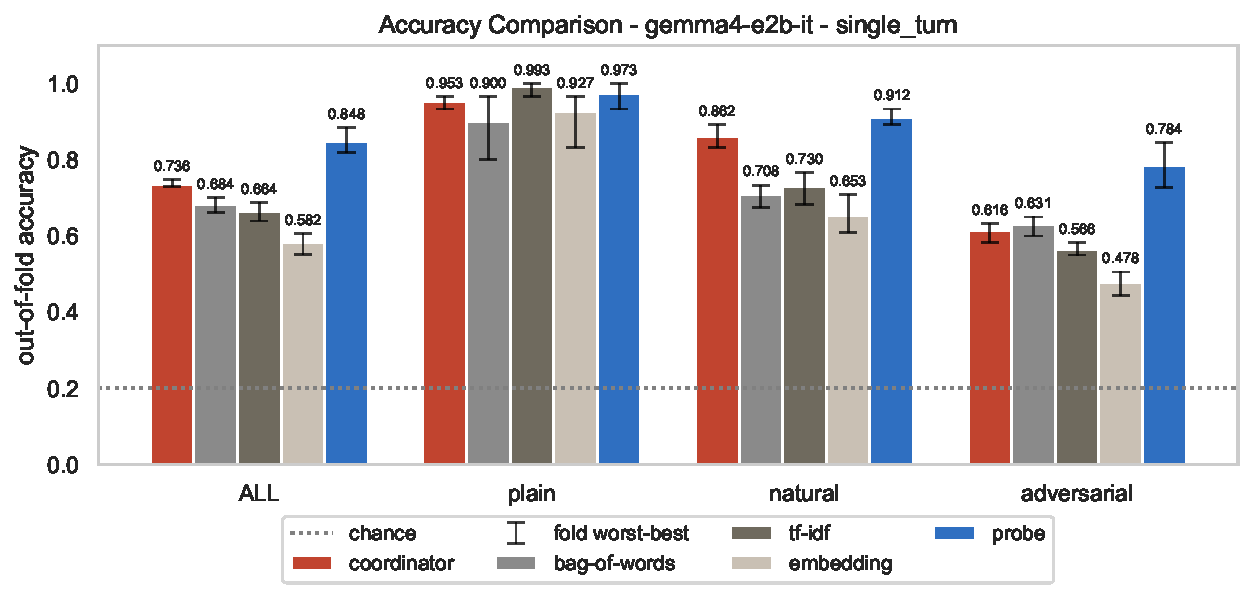
\includegraphics[width=0.85\textwidth]{images/models/gemma4-e2b-it_single_turn_routers.pdf}
    \caption[Accuracy comparison, gemma4-e2b-it, single-turn]{Accuracy comparison, gemma4-e2b-it, single-turn.}
    \label{fig:ch7-gemma4-e2b-it-single-routers}
\end{figure}

\begin{figure}[H]
    \centering
    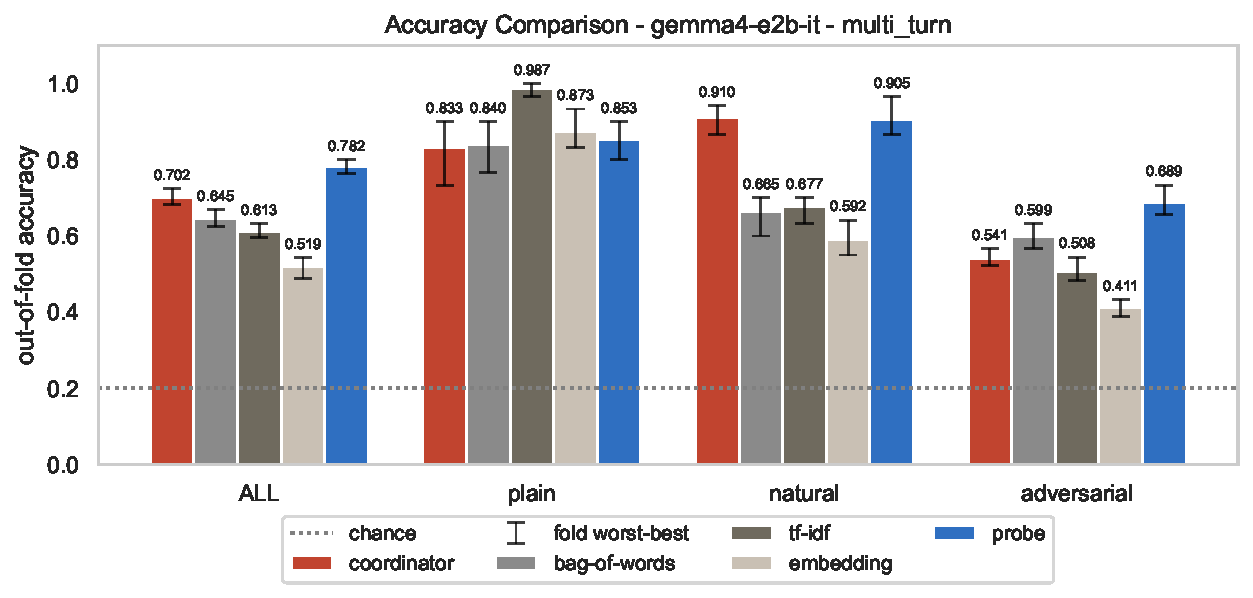
\includegraphics[width=0.85\textwidth]{images/models/gemma4-e2b-it_multi_turn_routers.pdf}
    \caption[Accuracy comparison, gemma4-e2b-it, multi-turn]{Accuracy comparison, gemma4-e2b-it, multi-turn.}
    \label{fig:ch7-gemma4-e2b-it-multi-routers}
\end{figure}


\clearpage

\subsection{Qwen3 4B Instruct 2507}
\label{subsec:ch7-qwen3-4b}

\begin{table}[H]
    \centering
    \small
    \setlength{\tabcolsep}{3.5pt}
    \begin{tabular}{@{}lcccccccccc@{}}
        \toprule
        & & & \multicolumn{4}{c}{\textbf{all}} & \multicolumn{4}{c}{\textbf{adversarial}} \\
        \cmidrule(lr){4-7} \cmidrule(lr){8-11}
        & \textbf{optimal layer} & \textbf{AUC macro} & \textbf{model} & \textbf{probe} & $\boldsymbol{\Delta}$ & $\boldsymbol{p_{\text{holm}}}$ & \textbf{model} & \textbf{probe} & $\boldsymbol{\Delta}$ & $\boldsymbol{p_{\text{holm}}}$ \\
        \midrule
        Single-turn & 23/36 & 0.977 & 0.752 & 0.864 & \rgain{0.112} & $<10^{-4}$ & 0.610 & 0.806 & \rgain{0.196} & $<10^{-4}$ \\
        Multi-turn & 23/36 & 0.959 & 0.745 & 0.814 & \rgain{0.069} & $<10^{-4}$ & 0.602 & 0.718 & \rgain{0.116} & $<10^{-4}$ \\
        \bottomrule
    \end{tabular}
    \caption[\texttt{qwen3-4b}, probe against model, both datasets]{\texttt{qwen3-4b}, probe against model, both datasets.}
    \label{tab:ch7-qwen3-4b}
\end{table}

\begin{figure}[H]
    \centering
    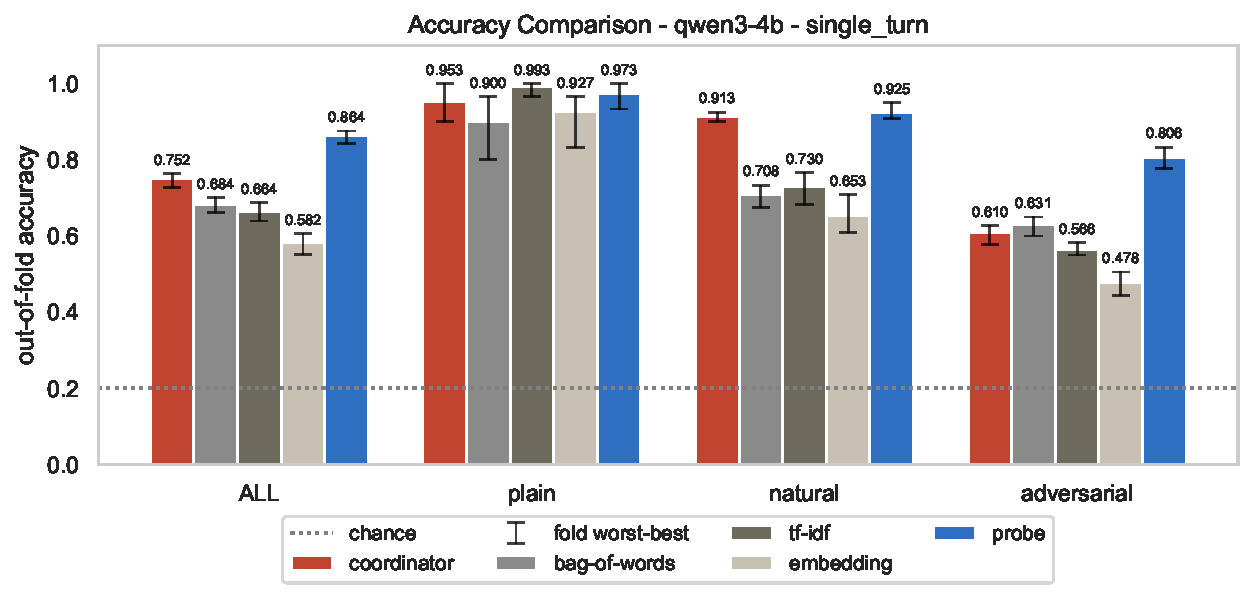
\includegraphics[width=0.85\textwidth]{images/models/qwen3-4b_single_turn_routers.pdf}
    \caption[Accuracy comparison, qwen3-4b, single-turn]{Accuracy comparison, qwen3-4b, single-turn.}
    \label{fig:ch7-qwen3-4b-single-routers}
\end{figure}

\begin{figure}[H]
    \centering
    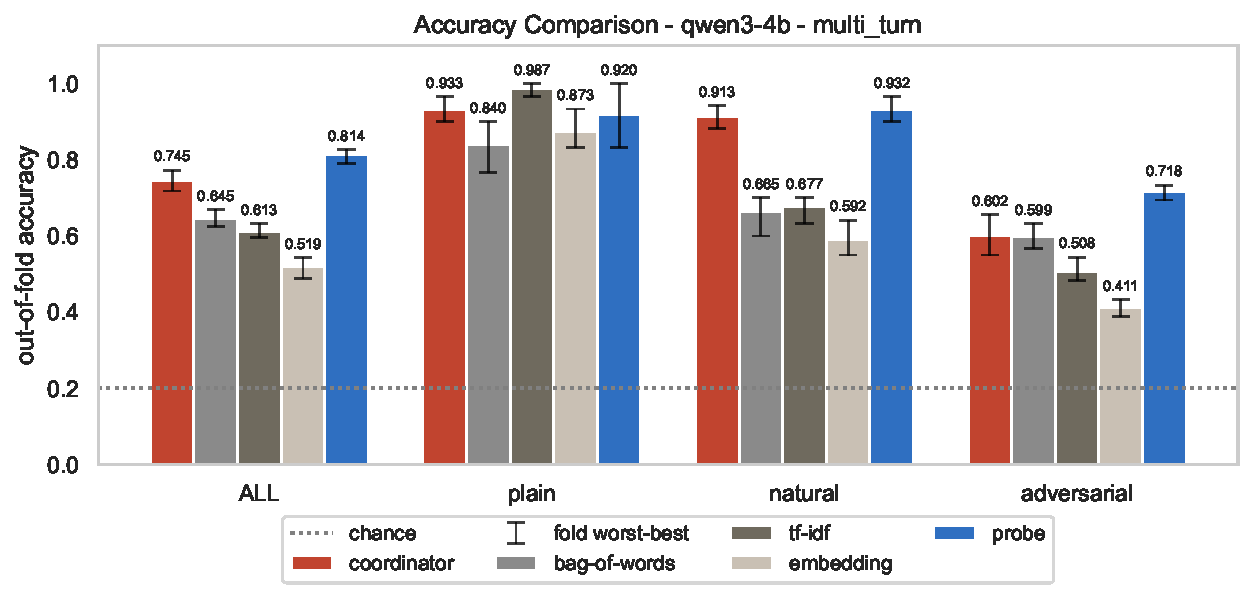
\includegraphics[width=0.85\textwidth]{images/models/qwen3-4b_multi_turn_routers.pdf}
    \caption[Accuracy comparison, qwen3-4b, multi-turn]{Accuracy comparison, qwen3-4b, multi-turn.}
    \label{fig:ch7-qwen3-4b-multi-routers}
\end{figure}


\clearpage

\subsection{Qwen3 8B}
\label{subsec:ch7-qwen3-8b}

\begin{table}[H]
    \centering
    \small
    \setlength{\tabcolsep}{3.5pt}
    \begin{tabular}{@{}lcccccccccc@{}}
        \toprule
        & & & \multicolumn{4}{c}{\textbf{all}} & \multicolumn{4}{c}{\textbf{adversarial}} \\
        \cmidrule(lr){4-7} \cmidrule(lr){8-11}
        & \textbf{optimal layer} & \textbf{AUC macro} & \textbf{model} & \textbf{probe} & $\boldsymbol{\Delta}$ & $\boldsymbol{p_{\text{holm}}}$ & \textbf{model} & \textbf{probe} & $\boldsymbol{\Delta}$ & $\boldsymbol{p_{\text{holm}}}$ \\
        \midrule
        Single-turn & 23/36 & 0.974 & 0.772 & 0.845 & \rgain{0.073} & $<10^{-4}$ & 0.652 & 0.784 & \rgain{0.132} & $<10^{-4}$ \\
        Multi-turn & 30/36 & 0.928 & 0.738 & 0.744 & \rgain{0.006} & \pns{0.65} & 0.597 & 0.634 & \rgain{0.037} & \pns{0.10} \\
        \bottomrule
    \end{tabular}
    \caption[\texttt{qwen3-8b}, probe against model, both datasets]{\texttt{qwen3-8b}, probe against model, both datasets.}
    \label{tab:ch7-qwen3-8b}
\end{table}

\begin{figure}[H]
    \centering
    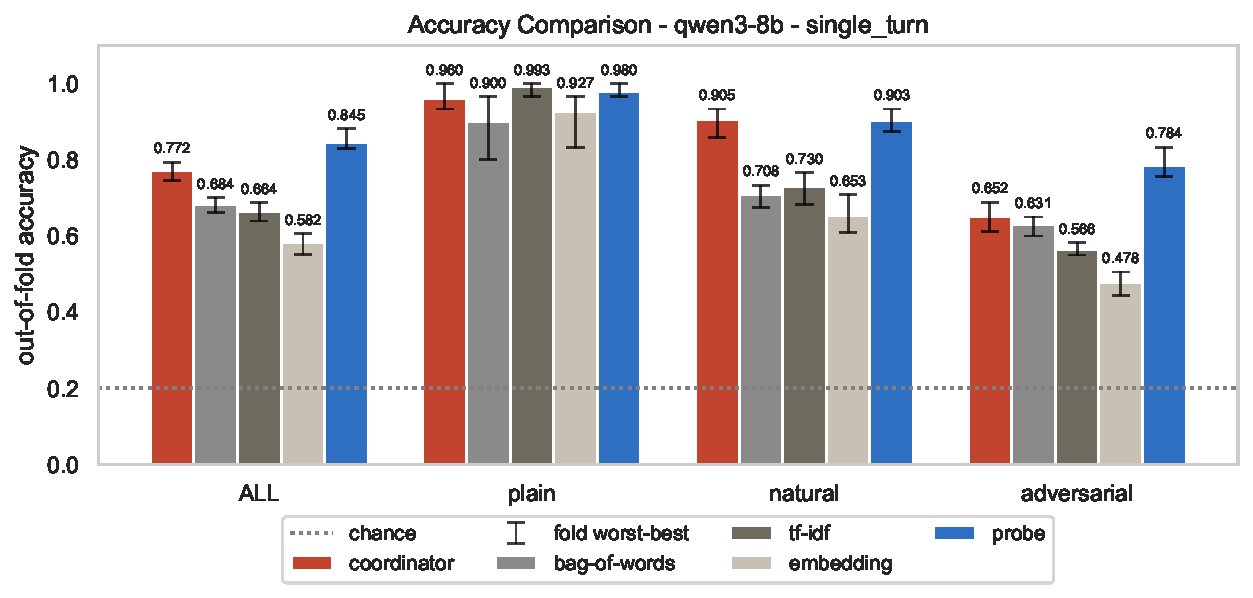
\includegraphics[width=0.85\textwidth]{images/models/qwen3-8b_single_turn_routers.pdf}
    \caption[Accuracy comparison, qwen3-8b, single-turn]{Accuracy comparison, qwen3-8b, single-turn.}
    \label{fig:ch7-qwen3-8b-single-routers}
\end{figure}

\begin{figure}[H]
    \centering
    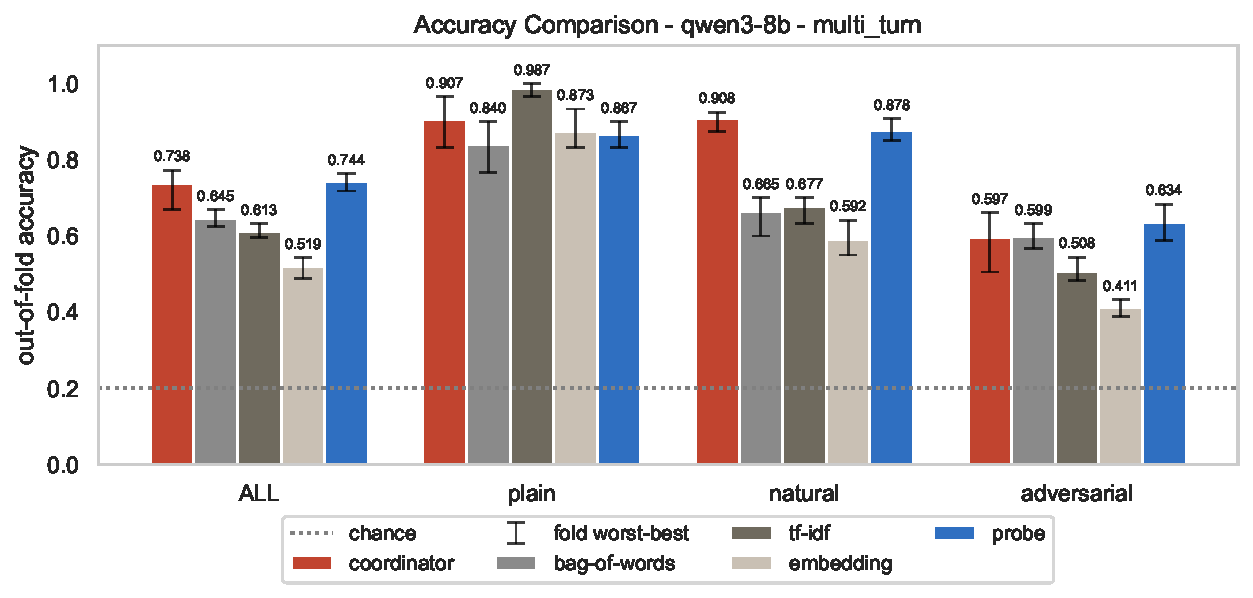
\includegraphics[width=0.85\textwidth]{images/models/qwen3-8b_multi_turn_routers.pdf}
    \caption[Accuracy comparison, qwen3-8b, multi-turn]{Accuracy comparison, qwen3-8b, multi-turn.}
    \label{fig:ch7-qwen3-8b-multi-routers}
\end{figure}


\clearpage

\subsection{Gemma 4 12B IT}
\label{subsec:ch7-gemma4-12b-it}

\begin{table}[H]
    \centering
    \small
    \setlength{\tabcolsep}{3.5pt}
    \begin{tabular}{@{}lcccccccccc@{}}
        \toprule
        & & & \multicolumn{4}{c}{\textbf{all}} & \multicolumn{4}{c}{\textbf{adversarial}} \\
        \cmidrule(lr){4-7} \cmidrule(lr){8-11}
        & \textbf{optimal layer} & \textbf{AUC macro} & \textbf{model} & \textbf{probe} & $\boldsymbol{\Delta}$ & $\boldsymbol{p_{\text{holm}}}$ & \textbf{model} & \textbf{probe} & $\boldsymbol{\Delta}$ & $\boldsymbol{p_{\text{holm}}}$ \\
        \midrule
        Single-turn & 31/48 & 0.988 & 0.873 & 0.916 & \rgain{0.043} & $<10^{-4}$ & 0.829 & 0.884 & \rgain{0.055} & $<10^{-4}$ \\
        Multi-turn & 32/48 & 0.979 & 0.855 & 0.879 & \rgain{0.024} & 0.011 & 0.777 & 0.827 & \rgain{0.050} & 0.00048 \\
        \bottomrule
    \end{tabular}
    \caption[\texttt{gemma4-12b-it}, probe against model, both datasets]{\texttt{gemma4-12b-it}, probe against model, both datasets.}
    \label{tab:ch7-gemma4-12b-it}
\end{table}

\begin{figure}[H]
    \centering
    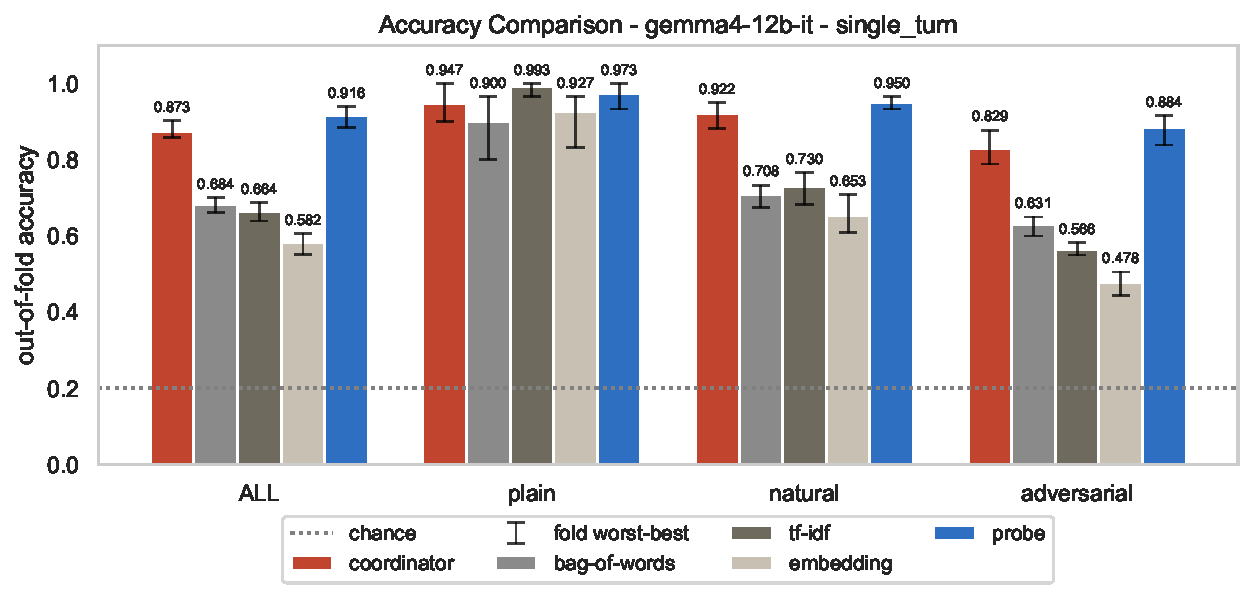
\includegraphics[width=0.85\textwidth]{images/models/gemma4-12b-it_single_turn_routers.pdf}
    \caption[Accuracy comparison, gemma4-12b-it, single-turn]{Accuracy comparison, gemma4-12b-it, single-turn.}
    \label{fig:ch7-gemma4-12b-it-single-routers}
\end{figure}

\begin{figure}[H]
    \centering
    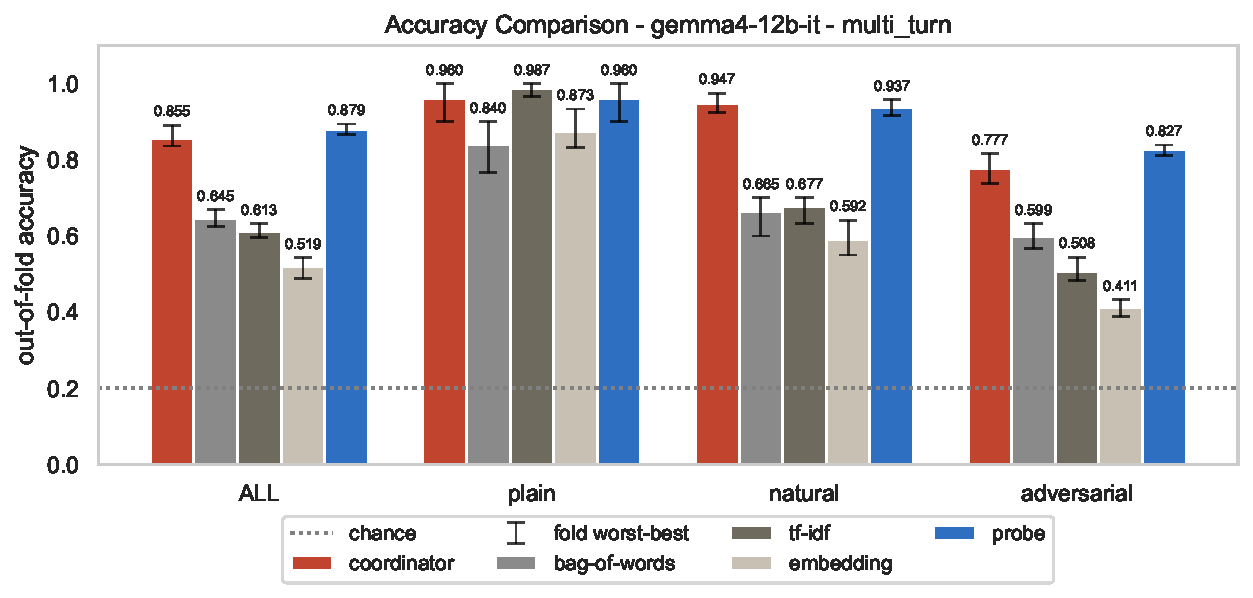
\includegraphics[width=0.85\textwidth]{images/models/gemma4-12b-it_multi_turn_routers.pdf}
    \caption[Accuracy comparison, gemma4-12b-it, multi-turn]{Accuracy comparison, gemma4-12b-it, multi-turn.}
    \label{fig:ch7-gemma4-12b-it-multi-routers}
\end{figure}


\clearpage

\subsection{GPT-OSS 20B}
\label{subsec:ch7-gpt-oss-20b}

\begin{table}[H]
    \centering
    \small
    \setlength{\tabcolsep}{3.5pt}
    \begin{tabular}{@{}lcccccccccc@{}}
        \toprule
        & & & \multicolumn{4}{c}{\textbf{all}} & \multicolumn{4}{c}{\textbf{adversarial}} \\
        \cmidrule(lr){4-7} \cmidrule(lr){8-11}
        & \textbf{optimal layer} & \textbf{AUC macro} & \textbf{model} & \textbf{probe} & $\boldsymbol{\Delta}$ & $\boldsymbol{p_{\text{holm}}}$ & \textbf{model} & \textbf{probe} & $\boldsymbol{\Delta}$ & $\boldsymbol{p_{\text{holm}}}$ \\
        \midrule
        Single-turn & 18/24 & 0.915 & 0.818 & 0.689 & \rgain{-0.129} & $<10^{-4}$ & 0.737 & 0.601 & \rgain{-0.136} & $<10^{-4}$ \\
        Multi-turn & 18/24 & 0.788 & 0.719 & 0.505 & \rgain{-0.214} & $<10^{-4}$ & 0.607 & 0.438 & \rgain{-0.169} & $<10^{-4}$ \\
        \bottomrule
    \end{tabular}
    \caption[\texttt{gpt-oss-20b}, probe against model, both datasets]{\texttt{gpt-oss-20b}, probe against model, both datasets.}
    \label{tab:ch7-gpt-oss-20b}
\end{table}

\begin{figure}[H]
    \centering
    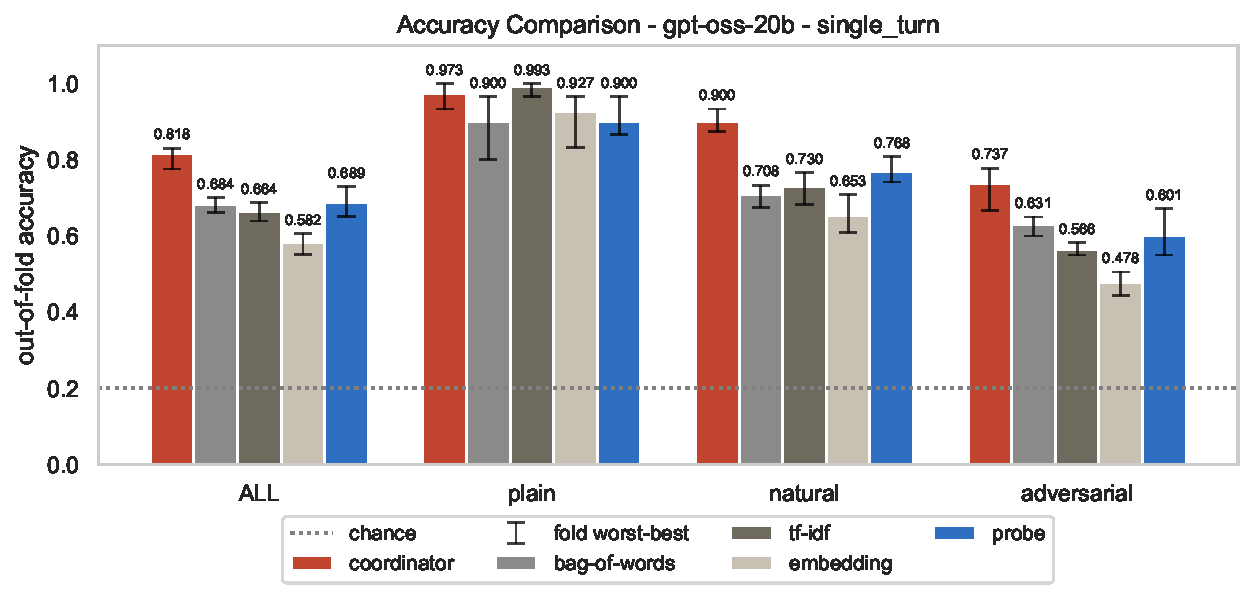
\includegraphics[width=0.85\textwidth]{images/models/gpt-oss-20b_single_turn_routers.pdf}
    \caption[Accuracy comparison, gpt-oss-20b, single-turn]{Accuracy comparison, gpt-oss-20b, single-turn.}
    \label{fig:ch7-gpt-oss-20b-single-routers}
\end{figure}

\begin{figure}[H]
    \centering
    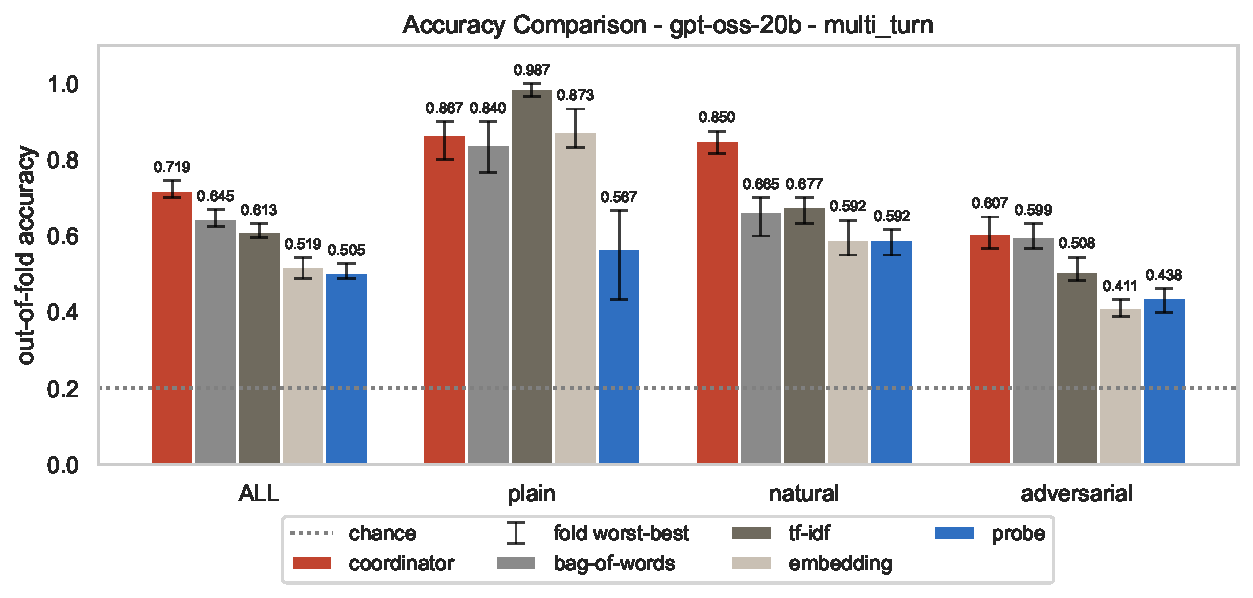
\includegraphics[width=0.85\textwidth]{images/models/gpt-oss-20b_multi_turn_routers.pdf}
    \caption[Accuracy comparison, gpt-oss-20b, multi-turn]{Accuracy comparison, gpt-oss-20b, multi-turn.}
    \label{fig:ch7-gpt-oss-20b-multi-routers}
\end{figure}


\clearpage

\subsection{Gemma 4 26B A4B IT}
\label{subsec:ch7-gemma4-26b-a4b-it}

\begin{table}[H]
    \centering
    \small
    \setlength{\tabcolsep}{3.5pt}
    \begin{tabular}{@{}lcccccccccc@{}}
        \toprule
        & & & \multicolumn{4}{c}{\textbf{all}} & \multicolumn{4}{c}{\textbf{adversarial}} \\
        \cmidrule(lr){4-7} \cmidrule(lr){8-11}
        & \textbf{optimal layer} & \textbf{AUC macro} & \textbf{model} & \textbf{probe} & $\boldsymbol{\Delta}$ & $\boldsymbol{p_{\text{holm}}}$ & \textbf{model} & \textbf{probe} & $\boldsymbol{\Delta}$ & $\boldsymbol{p_{\text{holm}}}$ \\
        \midrule
        Single-turn & 19/30 & 0.989 & 0.888 & 0.921 & \rgain{0.033} & 0.00012 & 0.841 & 0.888 & \rgain{0.047} & 0.001 \\
        Multi-turn & 19/30 & 0.977 & 0.856 & 0.878 & \rgain{0.022} & 0.024 & 0.773 & 0.831 & \rgain{0.058} & 0.00016 \\
        \bottomrule
    \end{tabular}
    \caption[\texttt{gemma4-26b-a4b-it}, probe against model, both datasets]{\texttt{gemma4-26b-a4b-it}, probe against model, both datasets.}
    \label{tab:ch7-gemma4-26b-a4b-it}
\end{table}

\begin{figure}[H]
    \centering
    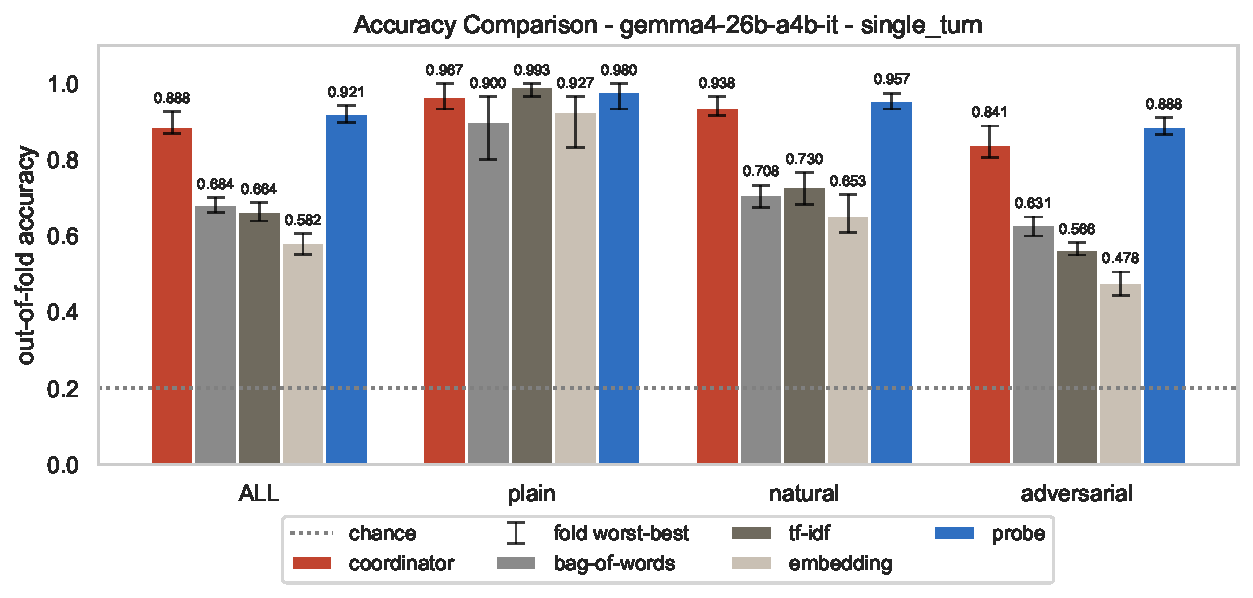
\includegraphics[width=0.85\textwidth]{images/models/gemma4-26b-a4b-it_single_turn_routers.pdf}
    \caption[Accuracy comparison, gemma4-26b-a4b-it, single-turn]{Accuracy comparison, gemma4-26b-a4b-it, single-turn.}
    \label{fig:ch7-gemma4-26b-a4b-it-single-routers}
\end{figure}

\begin{figure}[H]
    \centering
    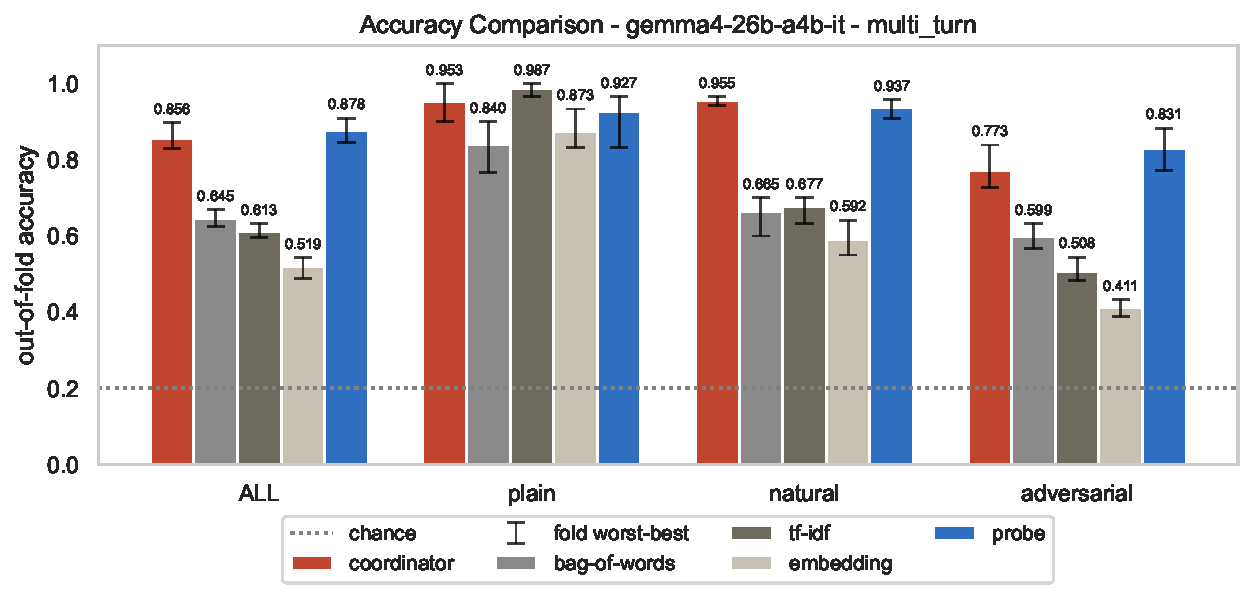
\includegraphics[width=0.85\textwidth]{images/models/gemma4-26b-a4b-it_multi_turn_routers.pdf}
    \caption[Accuracy comparison, gemma4-26b-a4b-it, multi-turn]{Accuracy comparison, gemma4-26b-a4b-it, multi-turn.}
    \label{fig:ch7-gemma4-26b-a4b-it-multi-routers}
\end{figure}


\clearpage

\subsection{Llama 3.3 70B Instruct}
\label{subsec:ch7-llama33-70b}

\begin{table}[H]
    \centering
    \small
    \setlength{\tabcolsep}{3.5pt}
    \begin{tabular}{@{}lcccccccccc@{}}
        \toprule
        & & & \multicolumn{4}{c}{\textbf{all}} & \multicolumn{4}{c}{\textbf{adversarial}} \\
        \cmidrule(lr){4-7} \cmidrule(lr){8-11}
        & \textbf{optimal layer} & \textbf{AUC macro} & \textbf{model} & \textbf{probe} & $\boldsymbol{\Delta}$ & $\boldsymbol{p_{\text{holm}}}$ & \textbf{model} & \textbf{probe} & $\boldsymbol{\Delta}$ & $\boldsymbol{p_{\text{holm}}}$ \\
        \midrule
        Single-turn & 42/80 & 0.985 & 0.770 & 0.894 & \rgain{0.124} & $<10^{-4}$ & 0.667 & 0.847 & \rgain{0.180} & $<10^{-4}$ \\
        Multi-turn & 38/80 & 0.950 & 0.736 & 0.810 & \rgain{0.074} & $<10^{-4}$ & 0.606 & 0.714 & \rgain{0.108} & $<10^{-4}$ \\
        \bottomrule
    \end{tabular}
    \caption[\texttt{llama3.3-70b}, probe against model, both datasets]{\texttt{llama3.3-70b}, probe against model, both datasets.}
    \label{tab:ch7-llama33-70b}
\end{table}

\begin{figure}[H]
    \centering
    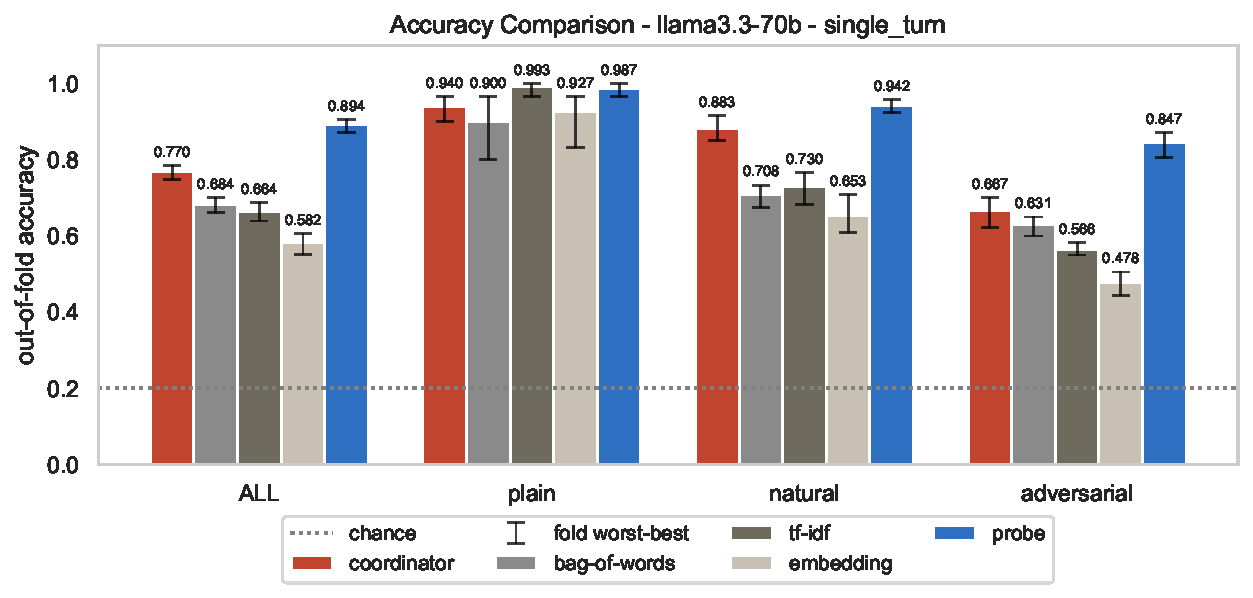
\includegraphics[width=0.85\textwidth]{images/models/llama33-70b_single_turn_routers.pdf}
    \caption[Accuracy comparison, llama3.3-70b, single-turn]{Accuracy comparison, llama3.3-70b, single-turn.}
    \label{fig:ch7-llama33-70b-single-routers}
\end{figure}

\begin{figure}[H]
    \centering
    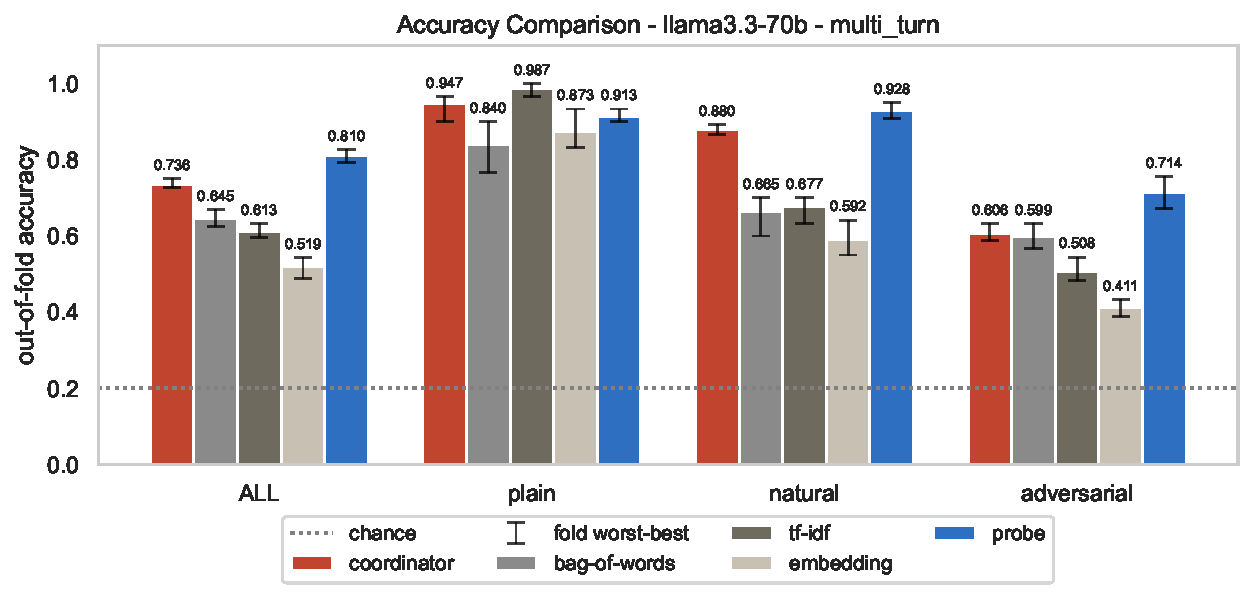
\includegraphics[width=0.85\textwidth]{images/models/llama33-70b_multi_turn_routers.pdf}
    \caption[Accuracy comparison, llama3.3-70b, multi-turn]{Accuracy comparison, llama3.3-70b, multi-turn.}
    \label{fig:ch7-llama33-70b-multi-routers}
\end{figure}


\clearpage

\subsection{Qwen2.5 72B Instruct}
\label{subsec:ch7-qwen25-72b}

\begin{table}[H]
    \centering
    \small
    \setlength{\tabcolsep}{3.5pt}
    \begin{tabular}{@{}lcccccccccc@{}}
        \toprule
        & & & \multicolumn{4}{c}{\textbf{all}} & \multicolumn{4}{c}{\textbf{adversarial}} \\
        \cmidrule(lr){4-7} \cmidrule(lr){8-11}
        & \textbf{optimal layer} & \textbf{AUC macro} & \textbf{model} & \textbf{probe} & $\boldsymbol{\Delta}$ & $\boldsymbol{p_{\text{holm}}}$ & \textbf{model} & \textbf{probe} & $\boldsymbol{\Delta}$ & $\boldsymbol{p_{\text{holm}}}$ \\
        \midrule
        Single-turn & 55/80 & 0.988 & 0.761 & 0.907 & \rgain{0.146} & $<10^{-4}$ & 0.638 & 0.862 & \rgain{0.224} & $<10^{-4}$ \\
        Multi-turn & 58/80 & 0.976 & 0.768 & 0.875 & \rgain{0.107} & $<10^{-4}$ & 0.629 & 0.800 & \rgain{0.171} & $<10^{-4}$ \\
        \bottomrule
    \end{tabular}
    \caption[\texttt{qwen2.5-72b}, probe against model, both datasets]{\texttt{qwen2.5-72b}, probe against model, both datasets.}
    \label{tab:ch7-qwen25-72b}
\end{table}

\begin{figure}[H]
    \centering
    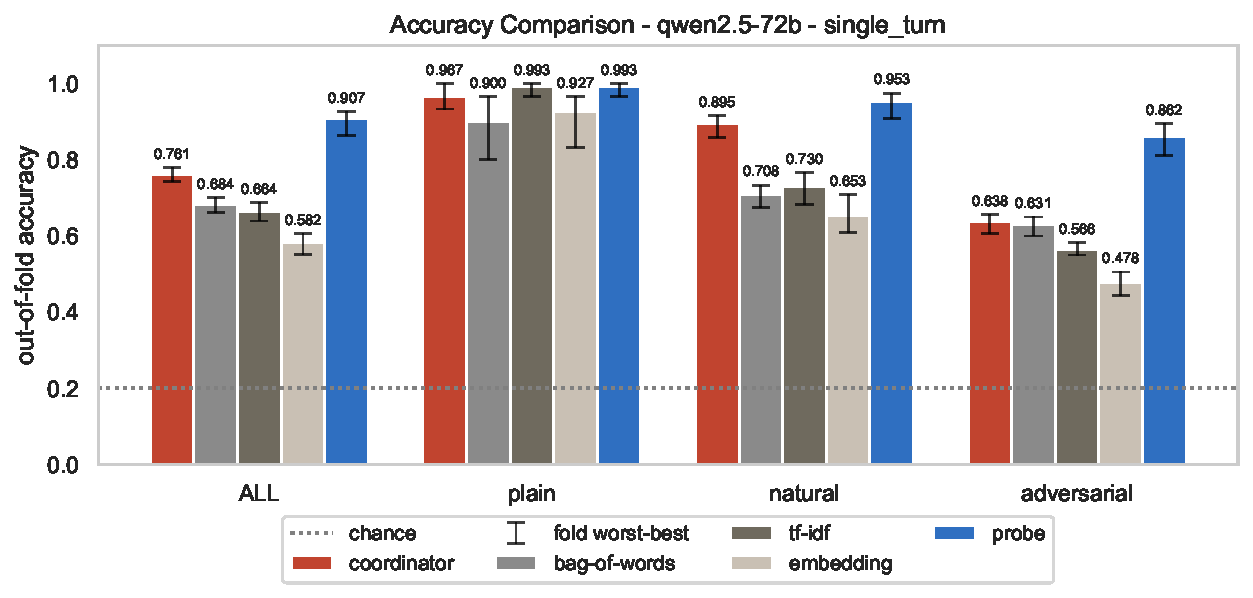
\includegraphics[width=0.85\textwidth]{images/models/qwen25-72b_single_turn_routers.pdf}
    \caption[Accuracy comparison, qwen2.5-72b, single-turn]{Accuracy comparison, qwen2.5-72b, single-turn.}
    \label{fig:ch7-qwen25-72b-single-routers}
\end{figure}

\begin{figure}[H]
    \centering
    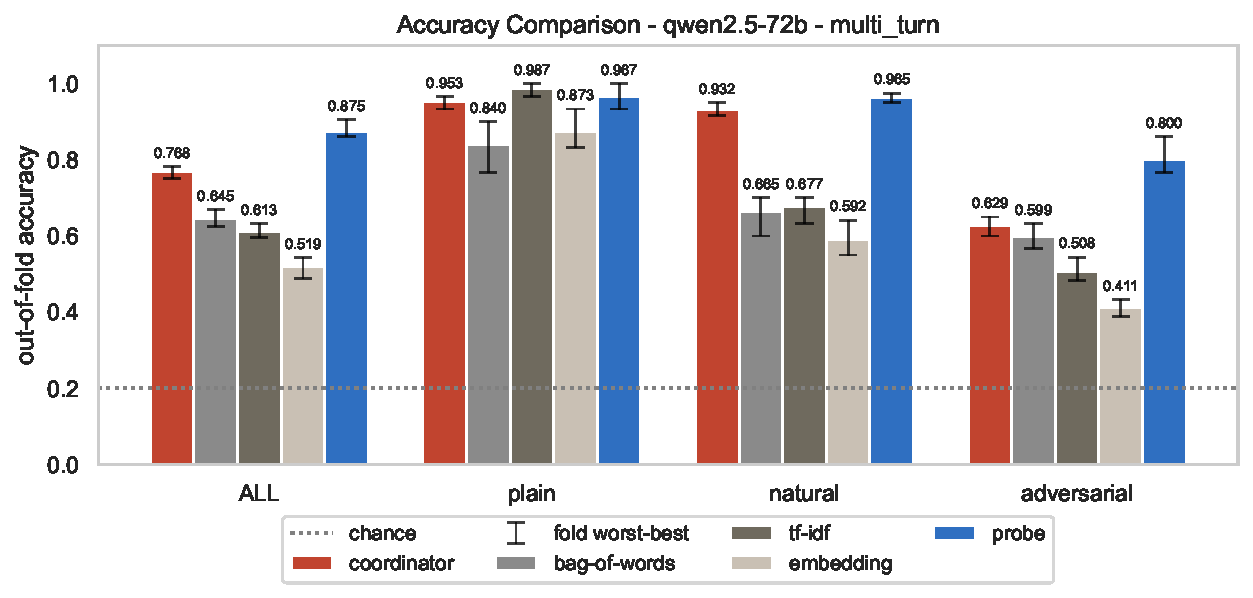
\includegraphics[width=0.85\textwidth]{images/models/qwen25-72b_multi_turn_routers.pdf}
    \caption[Accuracy comparison, qwen2.5-72b, multi-turn]{Accuracy comparison, qwen2.5-72b, multi-turn.}
    \label{fig:ch7-qwen25-72b-multi-routers}
\end{figure}



\clearpage
\section{Observations}
\label{sec:ch7-observations}

In all models except GPT-OSS 20B, the probe is more accurate than the model and than the three text-only classifiers, on both the whole single-turn and the whole multi-turn dataset. The difference between probe and model is significant according to the McNemar test, with one exception for Qwen3 8B on the whole multi-turn dataset ($p_{\text{holm}} = 0.65$). On the \texttt{plain} tier, the model, the probe and the text-only classifiers all score close to ceiling accuracy, and the TF-IDF classifier matches or exceeds the probe in every model. On the \texttt{natural} tier, the probe exceeds every text-only classifier by at least 0.17. On the single-turn dataset, it exceeds the model by 0.012 to 0.059 in six of the seven models, and it is 0.002 below the model for Qwen3 8B. On the \texttt{adversarial} tier, the accuracy of the probe exceeds the accuracy of every text-only classifier and of the model, on both datasets, and its difference from the model ranges from 0.037 to 0.224. This difference is significant in every model except Qwen3 8B on the multi-turn dataset ($p_{\text{holm}} = 0.10$). As the difficulty increases, the probe is the classifier that retains the most accuracy.

On the multi-turn dataset, the probe is less accurate than on the single-turn dataset in all eight models, and its AUC macro is also lower. This suggests that, in the multi-turn setting, the sub-agents are less clearly separable from the hidden states, making the classification harder for the probe. The model loses less accuracy between the two datasets, so the difference between probe and model is smaller on the multi-turn dataset.

GPT-OSS 20B, which is the third most accurate model on the single-turn dataset, is the exception to all the previous observations. Its probe is less accurate than its model on every tier of both datasets, and its AUC macro (0.915 single-turn, 0.788 multi-turn) is the lowest of the eight models. On the multi-turn dataset, its probe falls below the bag-of-words and the TF-IDF classifier on the whole dataset and on every tier. Among the eight models, GPT-OSS 20B is the only one whose reasoning cannot be disabled, so its routing decision may be formed after the last prompt token where the hidden states are probed.

Chapter~\ref{chap:results-analysis} analyzes these results in detail.


\chapter{Discussion of the Results}
\label{chap:results-analysis}

This chapter analyzes the results reported in Chapter~\ref{chap:probing-results} for each of the eight models and both datasets. Section~\ref{sec:ch8-gpt-oss} analyzes the results of GPT-OSS 20B separately, due to its difference from the other models stated in Chapter~\ref{chap:probing-results}, and because, among all the models, it is the only one where the results in Chapter~\ref{chap:probing-results} show a probe that is less accurate than the coordinator. The following sections then analyze the other seven models together.

Section~\ref{sec:ch8-overview} compares the probe against the coordinator, on the whole dataset, across the difficulty tiers and across the two interaction settings, and answers \hyperref[rq:ch8-rq1-intro]{\textbf{RQ1}}. Section~\ref{sec:ch8-failure-analysis} compares the failures of the probe, of the coordinator and of the text-only classifiers, and answers \hyperref[rq:ch8-rq2-intro]{\textbf{RQ2}}. Section~\ref{sec:ch8-depth} reports the relative depth of the optimal layer for the probe, and answers \hyperref[rq:ch8-rq3-intro]{\textbf{RQ3}}. Section~\ref{sec:ch8-error-flag} evaluates the probe as a runtime error flag on the coordinator's decision, and answers \hyperref[rq:ch8-rq4-intro]{\textbf{RQ4}}.

% many floats: let pages end short instead of stretching the text to the bottom
\raggedbottom

\section{Probe Underperformance on GPT-OSS 20B}
\label{sec:ch8-gpt-oss}

Among the eight models of Section~\ref{sec:ch7-results}, GPT-OSS 20B is the only one whose chain-of-thought output cannot be disabled (Section~\ref{subsec:ch7-reasoning-traces}). In its runs, a reasoning output is generated after the prompt and before the tool call that states the routing decision. GPT-OSS 20B is also the only model where the probe is less accurate than the coordinator. This section analyzes its two runs in detail, to determine whether the hidden state at the last prompt token may be insufficient to predict the choice of the sub-agent when the reasoning output cannot be disabled.

\begin{table}[htbp]
    \centering
    \begin{tabular}{@{}lcccc@{}}
        \toprule
        \textbf{Dataset} & \textbf{\begin{tabular}[b]{@{}c@{}}probe\\AUC macro\end{tabular}} & \textbf{\begin{tabular}[b]{@{}c@{}}probe AUC macro,\\other seven models\end{tabular}} & \textbf{\begin{tabular}[b]{@{}c@{}}coordinator\\accuracy\end{tabular}} & \textbf{\begin{tabular}[b]{@{}c@{}}probe\\accuracy\end{tabular}} \\
        \midrule
        Single-turn & 0.915 & 0.974--0.989 & \textbf{0.818} & 0.689 \\
        Multi-turn  & 0.788 & 0.928--0.979 & \textbf{0.719} & 0.505 \\
        \bottomrule
    \end{tabular}
    \caption[\texttt{gpt-oss-20b} probe AUC macro and coordinator accuracy]{\texttt{gpt-oss-20b}: AUC macro of the probe at its optimal layer, range of the same metric across the other seven models, accuracy of the coordinator and accuracy of the probe, from Section~\ref{sec:ch7-results}.}
    \label{tab:ch8-gpt-oss-exception}
\end{table}

Table~\ref{tab:ch8-gpt-oss-exception} shows that the accuracy of the probe is lower than the accuracy of the coordinator by 0.129 on the single-turn dataset and by 0.214 on the multi-turn dataset. On both datasets, the AUC macro of the probe is also below the range of the other seven models. The sub-agents are therefore less separable in the hidden states of GPT-OSS 20B than in those of any other model analyzed in this work.

\subsection{Probing at the Last Reasoning Token}
\label{subsec:ch8-gpt-oss-reasoning}

The probe reads the hidden state at the last prompt token, before the reasoning output is generated. For the other seven models the tool call follows the prompt directly, but for GPT-OSS 20B the choice of the sub-agent may be formed during the reasoning process. The representation at the last prompt token may therefore be insufficient to train a linear probe that can separate the sub-agents accurately.

To test this reading, a second simulation of GPT-OSS 20B was run on the single-turn dataset to capture the hidden states at the last token of the reasoning output. A probe was then trained on these hidden states at every layer, with the same procedure used at the last prompt token (Section~\ref{sec:ch7-probing-setup}). Table~\ref{tab:ch8-gpt-oss-reasoning} compares the probe at the last prompt token, reported in Section~\ref{subsec:ch7-gpt-oss-20b}, with the probe at the last reasoning token. Figure~\ref{fig:ch8-gpt-oss-reasoning-routers} compares the probe at the last reasoning token with the coordinator's decision and the text-only baselines, and its layer sweep is reported in Appendix~\ref{chap:appendix-layer-sweeps}.

\begin{table}[htbp]
    \centering
    \small
    \setlength{\tabcolsep}{3.5pt}
    \begin{tabular}{@{}lcccccccccc@{}}
        \toprule
        & & & \multicolumn{4}{c}{\textbf{all}} & \multicolumn{4}{c}{\textbf{adversarial}} \\
        \cmidrule(lr){4-7} \cmidrule(lr){8-11}
        & \textbf{optimal layer} & \textbf{AUC macro} & \textbf{model} & \textbf{probe} & $\boldsymbol{\Delta}$ & $\boldsymbol{p_{\text{holm}}}$ & \textbf{model} & \textbf{probe} & $\boldsymbol{\Delta}$ & $\boldsymbol{p_{\text{holm}}}$ \\
        \midrule
        Prompt & 18/24 & 0.915 & 0.818 & 0.689 & \rgain{-0.129} & $<10^{-4}$ & 0.737 & 0.601 & \rgain{-0.136} & $<10^{-4}$ \\
        Reasoning & 16/24 & 0.936 & 0.818 & 0.796 & \rgain{-0.022} & 0.026 & 0.737 & 0.719 & \rgain{-0.018} & \pns{0.20} \\
        \bottomrule
    \end{tabular}
    \caption[\texttt{gpt-oss-20b}, probe against model at the last prompt and reasoning token]{\texttt{gpt-oss-20b}, single-turn, probe against model at the last prompt token (Prompt) and at the last reasoning token (Reasoning). A $p_{\text{holm}}$ followed by (n.s.) is not significant at the 0.05 threshold.}
    \label{tab:ch8-gpt-oss-reasoning}
\end{table}

\begin{figure}[htbp]
    \centering
    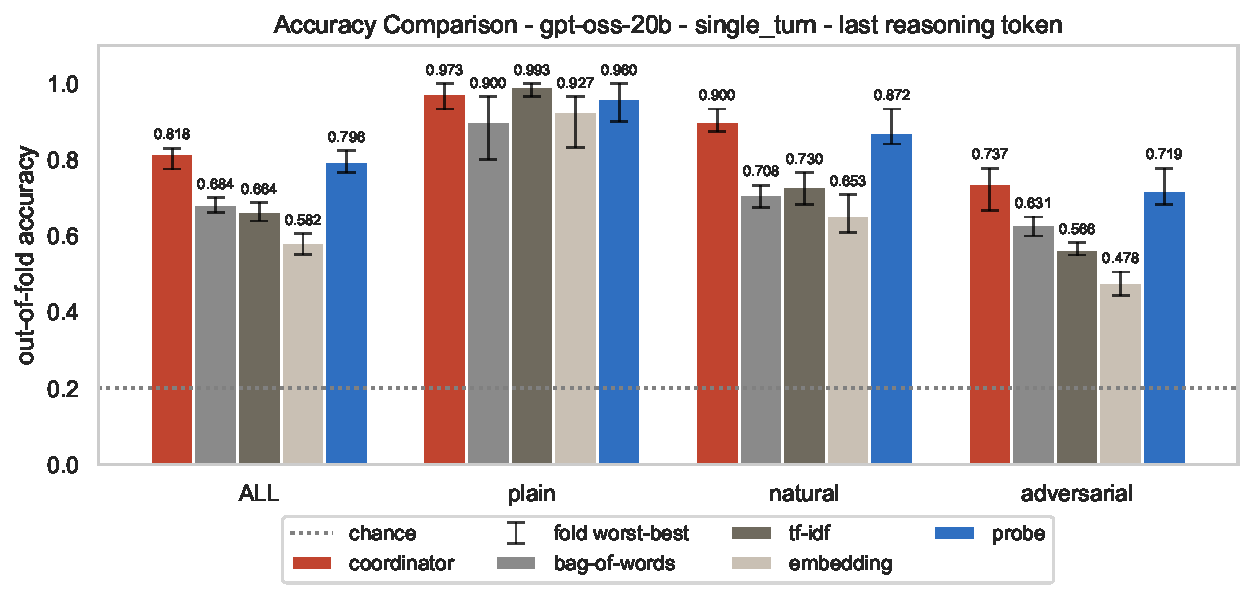
\includegraphics[width=0.85\textwidth]{images/models/gpt-oss-20b_single_turn_reasoning_routers.pdf}
    \caption[Accuracy comparison, gpt-oss-20b, single-turn, probe at the last reasoning token]{Accuracy comparison, gpt-oss-20b, single-turn, probe at the last reasoning token.}
    \label{fig:ch8-gpt-oss-reasoning-routers}
\end{figure}

\subsection{Observations}
\label{subsec:ch8-gpt-oss-observations}

At the last reasoning token, the AUC macro of the probe rises from 0.915 to 0.936. The accuracy of the probe rises from 0.689 to 0.796 on the whole dataset and from 0.601 to 0.719 on the \texttt{adversarial} tier. The probe exceeds all three text-only baselines on the whole dataset and on the \texttt{natural} and \texttt{adversarial} tiers, and its accuracy gets close to the accuracy of the coordinator without exceeding it. The accuracy of the coordinator exceeds the accuracy of the probe by 0.022 on the whole dataset and 0.018 on the \texttt{adversarial} tier. According to the McNemar test, the difference is significant on the whole dataset ($p_{\text{holm}} = 0.026$) but not on the \texttt{adversarial} tier ($p_{\text{holm}} = 0.20$).

A possible reason is that, before the last reasoning token, the model has already generated a reasoning output that discusses the sub-agents and reaches a conclusion. The hidden state during reasoning summarizes the input and the reasoning generated so far, and it is updated as the reasoning proceeds towards a final answer \cite{luStreamingHallucinationDetection2026}. The hidden state at the last reasoning token may therefore be skewed towards the sub-agent the model chose. This does not happen for the other seven models, where the probe reads the hidden state before any output is generated. This reading is consistent with the fraction of samples where the probe predicts the same sub-agent as the coordinator, which rises from 0.672 at the last prompt token to 0.866 at the last reasoning token. A probe trained from this state may therefore mostly learn the decision of the coordinator, including its errors, which would explain why its accuracy approaches the accuracy of the coordinator without exceeding it.

For GPT-OSS 20B, the hidden state at the last prompt token may not yet encode enough information to predict the choice of the sub-agent, because that choice depends on the reasoning generated afterward. The hidden state at the last reasoning token, in contrast, may already reflect that choice, since the reasoning that leads to it has already been generated.

\subsection{Effect on the Rest of the Analysis}
\label{subsec:ch8-gpt-oss-exclusion}

Both probe positions examined in this section have a limitation for GPT-OSS 20B. At the last prompt token, the hidden state may not yet encode the choice of the sub-agent, because that choice may be formed during the reasoning output. At the last reasoning token, the hidden state may already reflect that choice, so the probe may mostly learn the decision of the coordinator, including its errors.

The results of GPT-OSS 20B are therefore excluded from Sections~\ref{sec:ch8-overview} to~\ref{sec:ch8-error-flag}, so that they are not pooled with the results of the other seven models.

\FloatBarrier


\section{Comparison of Coordinator and Probe Accuracy}
\label{sec:ch8-overview}

\phantomsection\label{rq:ch8-rq1-intro}
\begin{rqbox}[RQ1]
On requests where the correct sub-agent is difficult to determine from the wording alone, does a probe on the hidden states of a coordinator model recover the correct sub-agent more accurately than the coordinator's own selection?
\end{rqbox}


\noindent To answer \hyperref[rq:ch8-rq1-intro]{\textbf{RQ1}}, this section compares the accuracy of the probe with the accuracy of the coordinator on both datasets and on each difficulty tier. The comparison across the difficulty tiers shows how the accuracy of the probe changes against the accuracy of the coordinator as the difficulty increases. The comparison between the two datasets shows how the multi-turn setting affects the accuracy.

The correct sub-agent is difficult to determine from the wording alone when text-only classifiers reach a low accuracy on the request (Section~\ref{subsec:lexical-separability}). The difficulty tiers lower this accuracy from \texttt{plain} to \texttt{adversarial} (Section~\ref{sec:dataset-baselines}).

\subsection{Accuracy on the Whole Dataset}
\label{subsec:ch8-overview-all}

Table~\ref{tab:ch8-overview} reports, from Section~\ref{sec:ch7-results}, the AUC macro of the probe, the accuracy of the coordinator and of the probe, their difference, and the McNemar test between the two, Holm-corrected as in Chapter~\ref{chap:probing-results}. The \emph{margin} $\Delta$ is the difference between the two accuracies, computed as the accuracy of the probe minus the accuracy of the coordinator.

\begin{table}[htbp]
    \centering
    \small
    \setlength{\tabcolsep}{4pt}
        \begin{tabular}{@{}lccccc@{}}
            \toprule
            \textbf{Model} & \textbf{\begin{tabular}[b]{@{}c@{}}probe\\AUC macro\end{tabular}} & \textbf{\begin{tabular}[b]{@{}c@{}}coordinator\\accuracy\end{tabular}} & \textbf{\begin{tabular}[b]{@{}c@{}}probe\\accuracy\end{tabular}} & $\boldsymbol{\Delta}$ & $\boldsymbol{p_{\text{holm}}}$ \\
            \midrule
            \multicolumn{6}{@{}l}{\textit{Single-turn}} \\
            \midrule
            \texttt{gemma4-e2b-it} & 0.976 & \worst{0.736} & 0.848 & \rgain{0.112} & $<10^{-4}$ \\
            \texttt{qwen3-4b} & 0.977 & 0.752 & 0.864 & \rgain{0.112} & $<10^{-4}$ \\
            \texttt{qwen3-8b} & 0.974 & 0.772 & \worst{0.845} & \rgain{0.073} & $<10^{-4}$ \\
            \texttt{gemma4-12b-it} & 0.988 & 0.873 & 0.916 & \rgain{0.043} & $<10^{-4}$ \\
            \texttt{gemma4-26b-a4b-it} & 0.989 & \best{0.888} & \best{0.921} & \rgain{0.033} & 0.00012 \\
            \texttt{llama3.3-70b} & 0.985 & 0.770 & 0.894 & \rgain{0.124} & $<10^{-4}$ \\
            \texttt{qwen2.5-72b} & 0.988 & 0.761 & 0.907 & \rgain{0.146} & $<10^{-4}$ \\
            \midrule
            \multicolumn{6}{@{}l}{\textit{Multi-turn}} \\
            \midrule
            \texttt{gemma4-e2b-it} & 0.947 & \worst{0.702} & 0.782 & \rgain{0.080} & $<10^{-4}$ \\
            \texttt{qwen3-4b} & 0.959 & 0.745 & 0.814 & \rgain{0.069} & $<10^{-4}$ \\
            \texttt{qwen3-8b} & 0.928 & 0.738 & \worst{0.744} & \rgain{0.006} & \pns{0.65} \\
            \texttt{gemma4-12b-it} & 0.979 & 0.855 & \best{0.879} & \rgain{0.024} & 0.011 \\
            \texttt{gemma4-26b-a4b-it} & 0.977 & \best{0.856} & 0.878 & \rgain{0.022} & 0.024 \\
            \texttt{llama3.3-70b} & 0.950 & 0.736 & 0.810 & \rgain{0.074} & $<10^{-4}$ \\
            \texttt{qwen2.5-72b} & 0.976 & 0.768 & 0.875 & \rgain{0.107} & $<10^{-4}$ \\
            \bottomrule
        \end{tabular}
    \caption[Per-model results, with the probe at its optimal layer]{Per-model results of Section~\ref{sec:ch7-results}, with the probe at its optimal layer. A $p_{\text{holm}}$ followed by (n.s.) is not significant at the 0.05 threshold. In each dataset, the highest accuracy of the coordinator and of the probe is in bold and the lowest is underlined.}
    \label{tab:ch8-overview}
\end{table}

Averaged over the seven models, the accuracy of the coordinator is 0.793 on the single-turn dataset and 0.771 on the multi-turn dataset, against 0.885 and 0.826 for the probe. The mean margin is therefore 0.092 on the single-turn dataset and 0.055 on the multi-turn dataset. The probe is more accurate than the coordinator in all the runs, and the McNemar test determines the difference to be significant in all but one, Qwen3 8B on the multi-turn dataset, where the margin is 0.006 ($p_{\text{holm}} = 0.65$).

On the single-turn dataset, the accuracy of the probe varies over a smaller range between models than the accuracy of the coordinator. Over the seven models, the accuracy of the probe is between 0.845 and 0.921, a range of 0.076, and the accuracy of the coordinator is between 0.736 and 0.888, a range of 0.152. On the multi-turn dataset the two ranges are close, 0.135 for the probe, between 0.744 and 0.879, and 0.154 for the coordinator, between 0.702 and 0.856.

The smallest margins belong to the models with the highest coordinator accuracy. On the single-turn dataset, Gemma 4 26B A4B IT and Gemma 4 12B IT have the two highest coordinator accuracies, 0.888 and 0.873, and the two smallest margins, 0.033 and 0.043, while the three largest margins, 0.112, 0.124 and 0.146, belong to models with a coordinator accuracy below 0.775. The multi-turn dataset shows the same relation, except for Qwen3 8B, whose margin of 0.006 comes from the lowest probe accuracy of the fourteen runs, 0.744 (Section~\ref{subsec:ch8-multi-turn}).

\FloatBarrier

\subsection{Accuracy Across the Difficulty Tiers}
\label{subsec:ch8-overview-tiers}

The samples of both datasets are divided into three difficulty tiers, from \texttt{plain} to \texttt{adversarial} (Section~\ref{subsec:difficulty-tiers}). Table~\ref{tab:ch8-tiers} reports the accuracy of the coordinator and of the probe on the whole dataset and on each tier, and the margin $\Delta$ between them. Each value is the mean of the seven runs on the same dataset. The last row of each dataset reports the \emph{tier drop}, the difference between the accuracy on \texttt{plain} and the one on \texttt{adversarial}.

\begin{table}[htbp]
    \centering
    \small
    \setlength{\tabcolsep}{10pt}
    \begin{tabular}{@{}llccc@{}}
        \toprule
        \textbf{Dataset} & \textbf{Tier} & \textbf{\begin{tabular}[b]{@{}c@{}}mean coordinator\\accuracy\end{tabular}} & \textbf{\begin{tabular}[b]{@{}c@{}}mean probe\\accuracy\end{tabular}} & \textbf{mean} $\boldsymbol{\Delta}$ \\
        \midrule
        Single-turn & \texttt{all}         & 0.793 & 0.885 & \rgain{0.092} \\
                    & \texttt{plain}       & 0.955 & 0.980 & \rgain{0.025} \\
                    & \texttt{natural}     & 0.903 & 0.935 & \rgain{0.032} \\
                    & \texttt{adversarial} & 0.693 & 0.836 & \rgain{0.143} \\
                    & \textit{tier drop}   & 0.262 & 0.144 & \\
        \midrule
        Multi-turn  & \texttt{all}         & 0.771 & 0.826 & \rgain{0.055} \\
                    & \texttt{plain}       & 0.927 & 0.915 & \rgain{-0.012} \\
                    & \texttt{natural}     & 0.921 & 0.926 & \rgain{0.005} \\
                    & \texttt{adversarial} & 0.646 & 0.745 & \rgain{0.099} \\
                    & \textit{tier drop}   & 0.281 & 0.170 & \\
        \bottomrule
    \end{tabular}
    \caption[Coordinator and probe accuracy across difficulty tiers]{Accuracy of the coordinator and of the probe on the whole dataset (\texttt{all}) and on each difficulty tier, with the margin $\Delta$. Each value is the mean of the seven runs on the same dataset. The tier drop is the difference between the accuracy on \texttt{plain} and the one on \texttt{adversarial}.}
    \label{tab:ch8-tiers}
\end{table}

Figure~\ref{fig:ch8-tiers} draws the same accuracies as two lines per dataset, together with the line of every single run.

\begin{figure}[htbp]
    \centering
    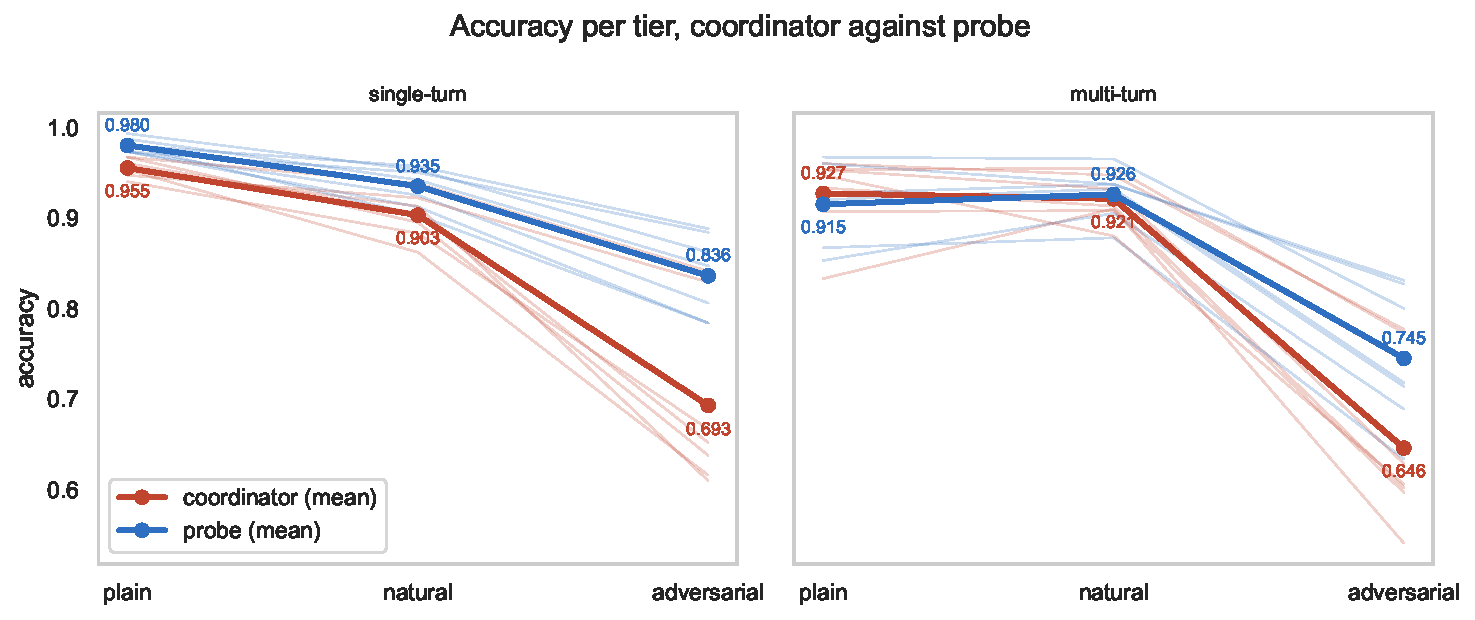
\includegraphics[width=\textwidth]{images/plots/overview/overview_tiers.pdf}
    \caption[Coordinator and probe accuracy across difficulty tiers]{Accuracy of the coordinator and of the probe on each difficulty tier, one panel per dataset. Thick lines are the mean over the seven models, thin lines are single runs. The tier drop is the fall of a line from \texttt{plain} to \texttt{adversarial}.}
    \label{fig:ch8-tiers}
\end{figure}
\FloatBarrier

The mean tier drop of the probe is 0.144 on the single-turn dataset and 0.170 on the multi-turn dataset, against 0.262 and 0.281 for the coordinator. The probe therefore loses less accuracy than the coordinator as the tier becomes harder, and the mean margin is largest on \texttt{adversarial}, 0.143 on the single-turn dataset and 0.099 on the multi-turn dataset. On the single-turn dataset, \texttt{plain} is the easiest tier and \texttt{adversarial} the hardest, for the coordinator and for the probe, in every model.

On the multi-turn dataset, the margin is positive in every model only on \texttt{adversarial}, where its mean is 0.099. On \texttt{plain} the margin is between $-$0.040 and 0.020, and the probe is more accurate than the coordinator in two of the seven models. On \texttt{natural} the margin is between $-$0.030 and 0.048, and the probe is more accurate than the coordinator in three of the seven models. The two tiers are not ordered by difficulty either. The probe is more accurate on \texttt{natural} than on \texttt{plain} in five of the seven models, and the coordinator is more accurate on \texttt{natural} than on \texttt{plain} in three of the seven models. The advantage of the probe on the multi-turn dataset therefore comes from \texttt{adversarial} alone, which holds 900 of the 1650 samples and contributes 0.054 of the mean margin of 0.055.

\FloatBarrier

\subsection{Accuracy Drop on the Multi-Turn Dataset}
\label{subsec:ch8-multi-turn}

The results of Chapter~\ref{chap:probing-results} show that the accuracy of the probe is lower on the multi-turn dataset than on the single-turn dataset for every model. Table~\ref{tab:ch8-multi-turn} reports, per model, the \emph{multi-turn drop} $\Delta_{mt}$ of the coordinator and of the probe, which is the accuracy on the multi-turn dataset minus the accuracy on the single-turn dataset. The table also reports the \emph{drop ratio}, which is the absolute multi-turn drop of the probe divided by the absolute multi-turn drop of the coordinator. The drop ratio is defined only where both multi-turn drops are negative, so it is reported for six of the seven models. The accuracies used to compute both quantities are the ones of Table~\ref{tab:ch8-overview}.

\begin{table}[htbp]
    \centering
    \small
    \begin{tabular}{@{}lccc c ccc c@{}}
        \toprule
        & \multicolumn{3}{c}{\textbf{coordinator accuracy}} & & \multicolumn{3}{c}{\textbf{probe accuracy}} & \\
        \cmidrule(lr){2-4} \cmidrule(lr){6-8}
        \textbf{Model} & \textbf{\begin{tabular}[b]{@{}c@{}}single-\\turn\end{tabular}} & \textbf{\begin{tabular}[b]{@{}c@{}}multi-\\turn\end{tabular}} & $\boldsymbol{\Delta_{mt}}$ & & \textbf{\begin{tabular}[b]{@{}c@{}}single-\\turn\end{tabular}} & \textbf{\begin{tabular}[b]{@{}c@{}}multi-\\turn\end{tabular}} & $\boldsymbol{\Delta_{mt}}$ & \textbf{\begin{tabular}[b]{@{}c@{}}drop\\ratio\end{tabular}} \\
        \midrule
        \texttt{gemma4-e2b-it}     & 0.736 & 0.702 & $-$0.034 & & 0.848 & 0.782 & $-$0.066 & 1.94 \\
        \texttt{qwen3-4b}          & 0.752 & 0.745 & $-$0.007 & & 0.864 & 0.814 & $-$0.050 & 7.14 \\
        \texttt{qwen3-8b}          & 0.772 & 0.738 & $-$0.034 & & 0.845 & 0.744 & $-$0.101 & 2.97 \\
        \texttt{gemma4-12b-it}     & 0.873 & 0.855 & $-$0.018 & & 0.916 & 0.879 & $-$0.037 & 2.06 \\
        \texttt{gemma4-26b-a4b-it} & 0.888 & 0.856 & $-$0.032 & & 0.921 & 0.878 & $-$0.043 & 1.34 \\
        \texttt{llama3.3-70b}      & 0.770 & 0.736 & $-$0.034 & & 0.894 & 0.810 & $-$0.084 & 2.47 \\
        \texttt{qwen2.5-72b}       & 0.761 & 0.768 & $+$0.007 & & 0.907 & 0.875 & $-$0.032 & N/A \\
        \bottomrule
    \end{tabular}
    \caption[Coordinator and probe accuracy across turns, with $\Delta_{mt}$]{Accuracy of the coordinator and of the probe on the single-turn and the multi-turn dataset, with the multi-turn drop $\Delta_{mt}$ and the drop ratio.}
    \label{tab:ch8-multi-turn}
\end{table}

Averaged over the seven models, the multi-turn drop is $-$0.022 for the coordinator and $-$0.059 for the probe. The multi-turn drop of the probe is larger in absolute value than the multi-turn drop of the coordinator in all seven models, including Qwen3 4B and Qwen2.5 72B, where the multi-turn drop of the coordinator accuracy is $-$0.007 and $+$0.007 but the multi-turn drop of the probe accuracy is $-$0.050 and $-$0.032. The drop ratio of Qwen2.5 72B is not defined, because its multi-turn drop of the coordinator is positive: the coordinator is more accurate on the multi-turn dataset than on the single-turn dataset, so the condition for the drop ratio, that both drops be negative, does not hold.

Figure~\ref{fig:ch8-multi-turn} draws the multi-turn drop $\Delta_{mt}$ of Table~\ref{tab:ch8-multi-turn} as one bar for the coordinator and one bar for the probe, per model.

\begin{figure}[htbp]
    \centering
    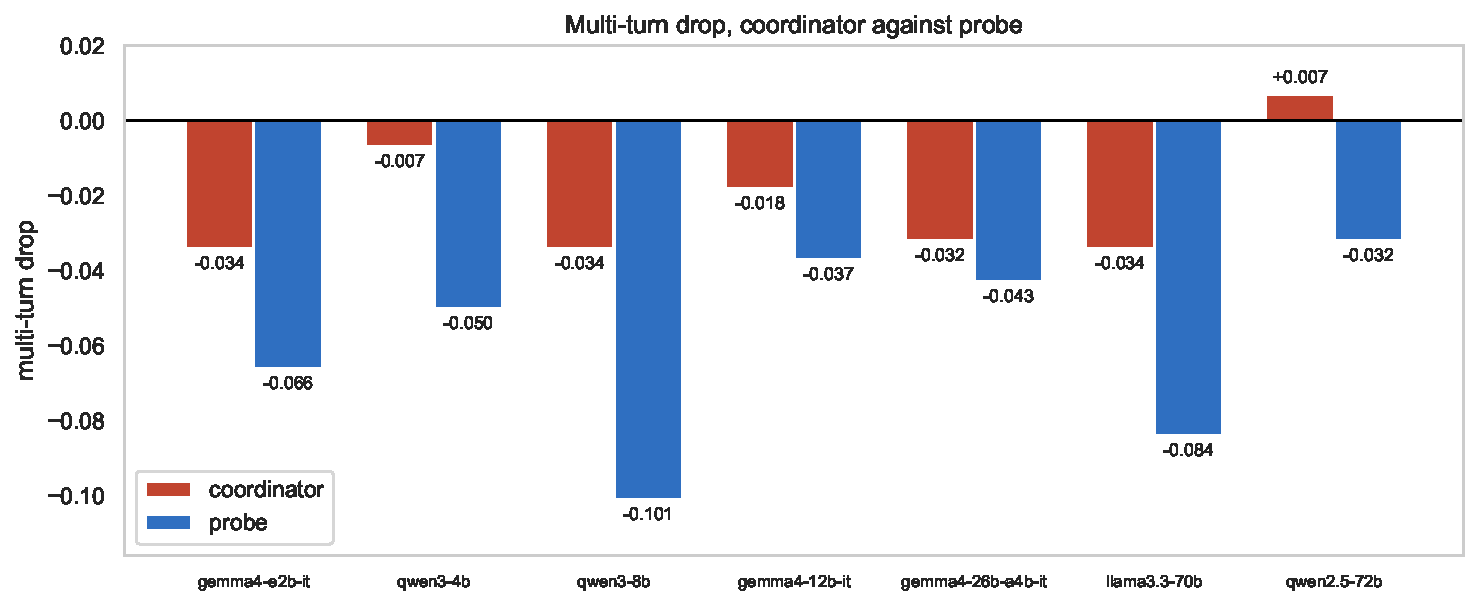
\includegraphics[width=\textwidth]{images/plots/overview/overview_multi_turn.pdf}
    \caption[Multi-turn drop $\Delta_{mt}$ of the coordinator and of the probe, per model]{Multi-turn drop $\Delta_{mt}$ of the coordinator and of the probe, per model. A bar below zero is a lower accuracy on the multi-turn dataset than on the single-turn dataset.}
    \label{fig:ch8-multi-turn}
\end{figure}

\FloatBarrier

\subsection{Answer to RQ1}
\label{subsec:ch8-rq1-answer}

\phantomsection\label{rq:ch8-rq1}
\begin{rqbox}[RQ1]
On requests where the correct sub-agent is difficult to determine from the wording alone, does a probe on the hidden states of a coordinator model recover the correct sub-agent more accurately than the coordinator's own selection?
\end{rqbox}


\noindent Yes. On both datasets and on every model of this section (GPT-OSS 20B excluded), the accuracy of the probe exceeds the accuracy of the coordinator, and the difference is significant in all the runs except Qwen3 8B on the multi-turn dataset, where the margin is 0.006. The mean margin is 0.092 on the single-turn dataset and 0.055 on the multi-turn dataset.

The advantage is largest on the \texttt{adversarial} tier, which is the difficulty tier where the correct sub-agent is the most difficult to determine from the wording of the request. On the single-turn dataset the mean margin grows from 0.025 on \texttt{plain} and 0.032 on \texttt{natural} to 0.143 on \texttt{adversarial}, and on the multi-turn dataset it grows from $-$0.012 and 0.005 to 0.099.

Every tier margin is lower in the multi-turn setting. The multi-turn drop $\Delta_{mt}$ of the probe is larger than the multi-turn drop of the coordinator in all seven models, $-$0.059 against $-$0.022 on average. A possible reason is that, in the multi-turn setting, the hidden state at the last prompt token provides a less separable representation of the sub-agents to train the probe on. Wu et al. report a similar loss of reliability while steering tool selection (adding a direction to the hidden state to change the tool the model calls): the effect becomes inconsistent once the conversation spans several turns \cite{wuToolCallingLinearly2026}.

\FloatBarrier


\section{Failure Analysis}
\label{sec:ch8-failure-analysis}

\phantomsection\label{rq:ch8-rq2-intro}
\begin{rqbox}[RQ2]
Does a probe on the coordinator's hidden states recover the correct sub-agent more accurately than classifiers trained on a fixed representation of the query text, such as raw word counts, TF-IDF weighting, or sentence embeddings?
\end{rqbox}


\noindent To answer \hyperref[rq:ch8-rq2-intro]{\textbf{RQ2}}, this section compares the probe with the three text-only classifiers on the \texttt{natural} and the \texttt{adversarial} tier. A request of the \texttt{natural} tier states a waived constraint, and the sub-agent that owns it is the decoy (Section~\ref{subsec:constraints-binding-waived}). The \texttt{adversarial} tier generates its requests in pairs: the two requests of a pair share most of their wording, and the correct sub-agent of each one is the decoy of the other (Section~\ref{subsec:difficulty-tiers}). The decoy and the pair are the cause of the lower accuracy of the text-only classifiers on these two tiers. The \texttt{plain} tier is deliberately excluded, because it introduces no difficulty and every text-only classifier scores close to ceiling accuracy on it.

The errors of the probe are first compared with the errors of each text-only classifier, to measure how much the two depend on each other. The probe, the coordinator and the text-only classifiers are then compared on how often each predicts the decoy, and on how often each predicts the same sub-agent for both requests of a pair. An advantage of the probe on these measures indicates that the binding constraint is encoded in the hidden states more accurately than in the representations of the request text that the text-only classifiers use.

\subsection{Error Dependence Across the Tiers}
\label{subsec:ch8-failure-dependence}

The errors of the probe are compared with the errors of the text-only classifiers to determine whether the hidden states encode information that the representations of the text-only classifiers do not encode. If the probe fails mostly on the same requests as a text-only classifier, its errors follow the text of the request as that classifier's errors do. If its errors are largely independent of the errors of the text-only classifiers, the hidden states are likely to encode information that these representations do not encode.

The coordinator is not included in this subsection because it is never trained on the requests of the dataset, unlike the probe and the text-only classifiers. The probe and the text-only classifiers are logistic regressions trained on the same labels and the same folds, and each receives a different input representation. A difference between their errors can therefore only come from this representation. A difference between the errors of the coordinator and the errors of a text-only classifier cannot be read the same way.

For each text-only classifier, the requests of a tier are divided into two groups: the requests where the text-only classifier is right and the requests where it is wrong. The following quantities are then computed for the probe, on each tier and against each text-only classifier:

\begin{itemize}
    \item \textbf{accuracy where the text-only classifier is right} ($a_p^{+}$): the accuracy of the probe on the requests where the text-only classifier is right;
    \item \textbf{accuracy where the text-only classifier is wrong} ($a_p^{-}$): the accuracy of the probe on the requests where the text-only classifier is wrong;
    \item \textbf{gap} ($g$): the difference $g = a_p^{-} - a_p^{+}$. A negative $g$ indicates that the probe is less accurate on the requests where the text-only classifier is wrong;
    \item \textbf{normalized kappa} ($\kappa_n$): measures how strongly the probe and the text-only classifier are right on the same requests and wrong on the same requests, on a scale from 0 for independent errors to 1 for the strongest agreement that the accuracies of the two allow.
\end{itemize}

The normalized kappa is derived from Cohen's kappa. For the probe and a text-only classifier, Cohen's kappa is computed as
\[
    \kappa = \frac{p_o - p_e}{1 - p_e},
\]
where:

\begin{itemize}
    \item $p_o$ is the fraction of requests on which the probe and the text-only classifier are both right or both wrong;
    \item $p_e$ is the value of $p_o$ expected from the accuracy of the probe and the accuracy of the text-only classifier if their errors were independent.
\end{itemize}

The highest value that $\kappa$ can reach depends on the accuracy $a_p$ of the probe and the accuracy $a_b$ of the text-only classifier. When the two accuracies differ, one of the two is right and the other is wrong on at least a fraction $|a_p - a_b|$ of the requests. Therefore $p_o$ is at most $1 - |a_p - a_b|$, and $\kappa$ is at most
\[
    \kappa_{\max} = \frac{1 - |a_p - a_b| - p_e}{1 - p_e}.
\]
The accuracies of the probe and of the text-only classifiers differ across text-only classifiers and tiers, so $\kappa_{\max}$ differs too, and the same value of $\kappa$ can indicate a weak agreement in one row of the comparison and a strong agreement in another. The normalized kappa removes this effect by dividing $\kappa$ by its highest reachable value:
\[
    \kappa_n = \frac{\kappa}{\kappa_{\max}}.
\]

If the errors of the probe do not depend on the errors of the text-only classifier, $g$ and $\kappa_n$ are close to 0 in absolute value. If the probe and the text-only classifier are right on the same requests and wrong on the same requests, $g$ is large and negative and $\kappa_n$ is close to 1. Table~\ref{tab:ch8-dependence} reports $a_p^{+}$, $a_p^{-}$, $g$ and $\kappa_n$ on the \texttt{natural} and \texttt{adversarial} tiers, and Figure~\ref{fig:ch8-dependence} plots $a_p^{+}$, $a_p^{-}$ and $g$.

In every row of Table~\ref{tab:ch8-dependence}, $a_p^{-}$ is lower than $a_p^{+}$, with $g$ between $-$0.028 and $-$0.179. Some of the requests on which the wording misleads the text-only classifiers therefore also mislead the probe. $\kappa_n$ between the probe and a text-only classifier is between 0.151 and 0.424. The absolute value of $g$ is larger on \texttt{adversarial} than on \texttt{natural} for every combination of dataset and text-only classifier. This shows that the difficulty of \texttt{adversarial} affects the probe more on the requests where a text-only classifier is wrong. Against the bag-of-words classifier, $\kappa_n$ is lower on \texttt{adversarial} than on \texttt{natural} on both datasets. Against the TF-IDF classifier, it is higher on the single-turn dataset and lower on the multi-turn dataset. Against the embedding classifier, it is higher on both datasets.

\begin{table}[H]
    \centering
    \small
    \begin{tabular}{@{}llcccc c cccc@{}}
        \toprule
        & & \multicolumn{4}{c}{\textbf{Single-turn}} & & \multicolumn{4}{c}{\textbf{Multi-turn}} \\
        \cmidrule(lr){3-6} \cmidrule(lr){8-11}
        \textbf{Tier} & \textbf{Classifier} & $\boldsymbol{a_p^{+}}$ & $\boldsymbol{a_p^{-}}$ & $\boldsymbol{g}$ & $\boldsymbol{\kappa_n}$ & & $\boldsymbol{a_p^{+}}$ & $\boldsymbol{a_p^{-}}$ & $\boldsymbol{g}$ & $\boldsymbol{\kappa_n}$ \\
        \midrule
        \texttt{natural}     & Bag-of-words & 0.958 & 0.878 & $-$0.080 & 0.356 & & \worst{0.944} & 0.891 & $-$0.053 & \worst{0.243} \\
                             & TF-IDF       & \best{0.959} & \worst{0.868} & \worst{$-$0.091} & \best{0.367} & & \best{0.950} & \worst{0.876} & \worst{$-$0.074} & \best{0.366} \\
                             & Embedding    & \worst{0.944} & \best{0.916} & \best{$-$0.028} & \worst{0.151} & & \worst{0.944} & \best{0.900} & \best{$-$0.044} & 0.268 \\
        \midrule
        \texttt{adversarial} & Bag-of-words & 0.888 & 0.749 & $-$0.139 & \worst{0.317} & & \worst{0.795} & 0.670 & \best{$-$0.125} & \worst{0.204} \\
                             & TF-IDF       & \best{0.905} & \worst{0.748} & \worst{$-$0.157} & \best{0.424} & & \best{0.833} & \worst{0.654} & \worst{$-$0.179} & \best{0.362} \\
                             & Embedding    & \worst{0.886} & \best{0.791} & \best{$-$0.095} & 0.321 & & 0.820 & \best{0.692} & $-$0.128 & 0.298 \\
        \bottomrule
    \end{tabular}
    \caption[Probe accuracy by classifier correctness, gap, and normalized kappa]{Accuracy of the probe on the requests where each text-only classifier is right ($a_p^{+}$) and on the requests where it is wrong ($a_p^{-}$), gap $g = a_p^{-} - a_p^{+}$, and normalized kappa $\kappa_n$ between the probe and the text-only classifier. Each value is the mean of the seven runs on the same dataset. In each tier and column, the highest value is in bold and the lowest is underlined.}
    \label{tab:ch8-dependence}
\end{table}

\begin{figure}[htbp]
    \centering
    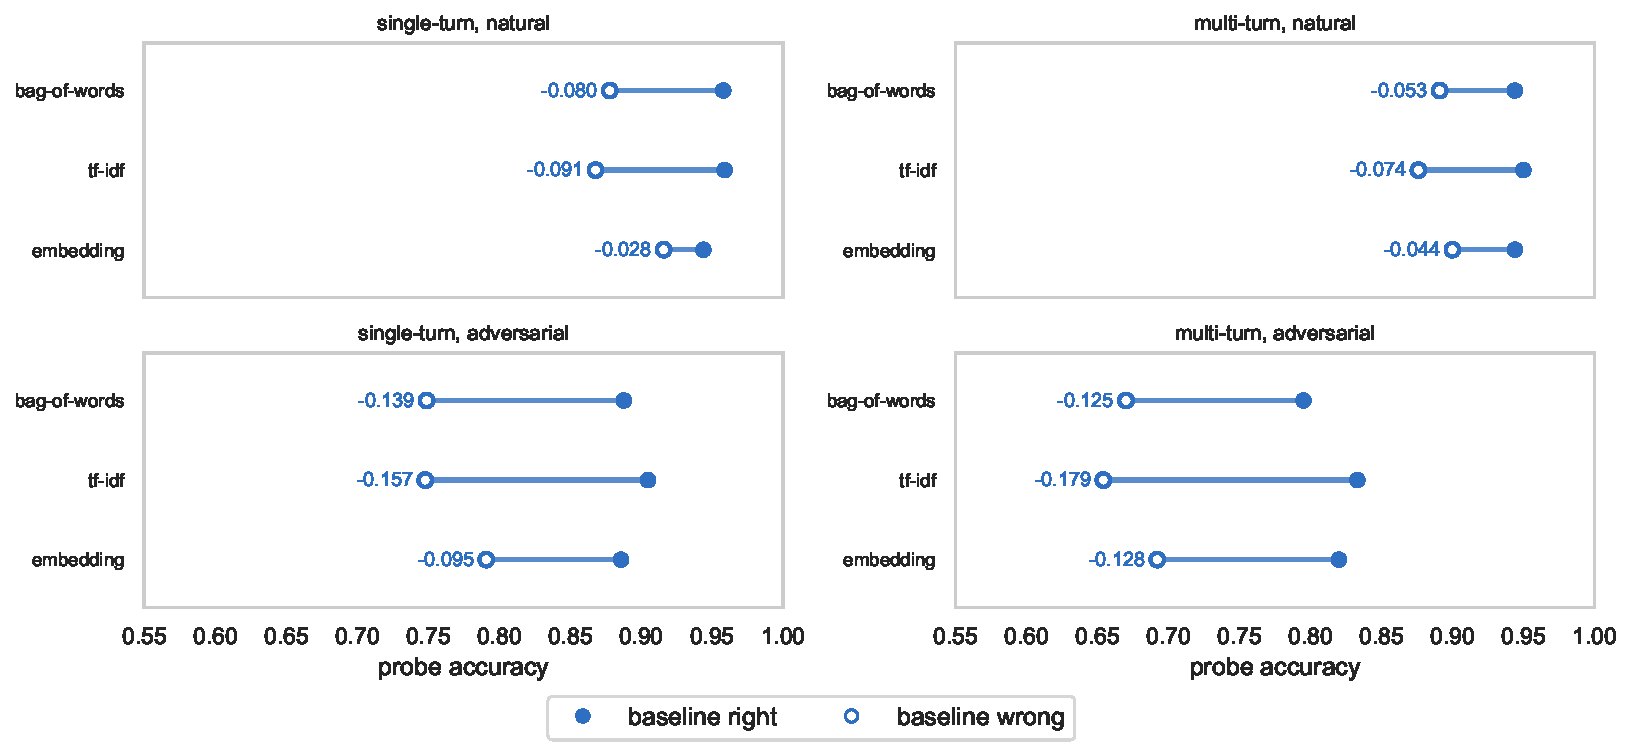
\includegraphics[width=\textwidth]{images/plots/overview/overview_dependence.pdf}
    \caption[Probe accuracy where each text-only classifier is right and where it is wrong]{Accuracy of the probe where each text-only classifier is right ($a_p^{+}$, filled end) and where it is wrong ($a_p^{-}$, hollow end), one panel per dataset and tier. The number at the hollow end is the gap $g$. Each value is the mean of the seven runs on the same dataset.}
    \label{fig:ch8-dependence}
\end{figure}

\FloatBarrier

\subsection{Adversarial Pairs}
\label{subsec:ch8-failure-pairs}

As described in Section~\ref{subsec:difficulty-tiers}, the \texttt{adversarial} tier of each dataset consists of 900 samples generated in 450 pairs. The two requests of a pair share most of their wording and differ only in the clause that names the constraint that is binding. Both requests state the same two constraints, and the constraint that is binding in one request is waived in the other, so the correct sub-agent of each request is the decoy of the other. The pairs are used to observe whether a classifier tells the two requests of a pair apart or predicts the same sub-agent for both, where a \emph{classifier} is any of the probe, the coordinator and the three text-only classifiers. Two quantities are computed for each classifier:

\begin{itemize}
    \item \textbf{both, one or neither right}: the share of pairs in which the classifier classifies both requests correctly, one of the two, or neither;
    \item \textbf{collapsed pairs}: the share of pairs in which the classifier predicts the same sub-agent for both requests. In a collapsed pair, at most one of the two requests is classified correctly.
\end{itemize}

Figure~\ref{fig:ch8-pairs} reports both quantities and shows that the probe is the only classifier that classifies both requests correctly in most pairs, on both datasets. The coordinator and the text-only classifiers classify only one of the two requests correctly in most pairs.

\begin{figure}[htbp]
    \centering
    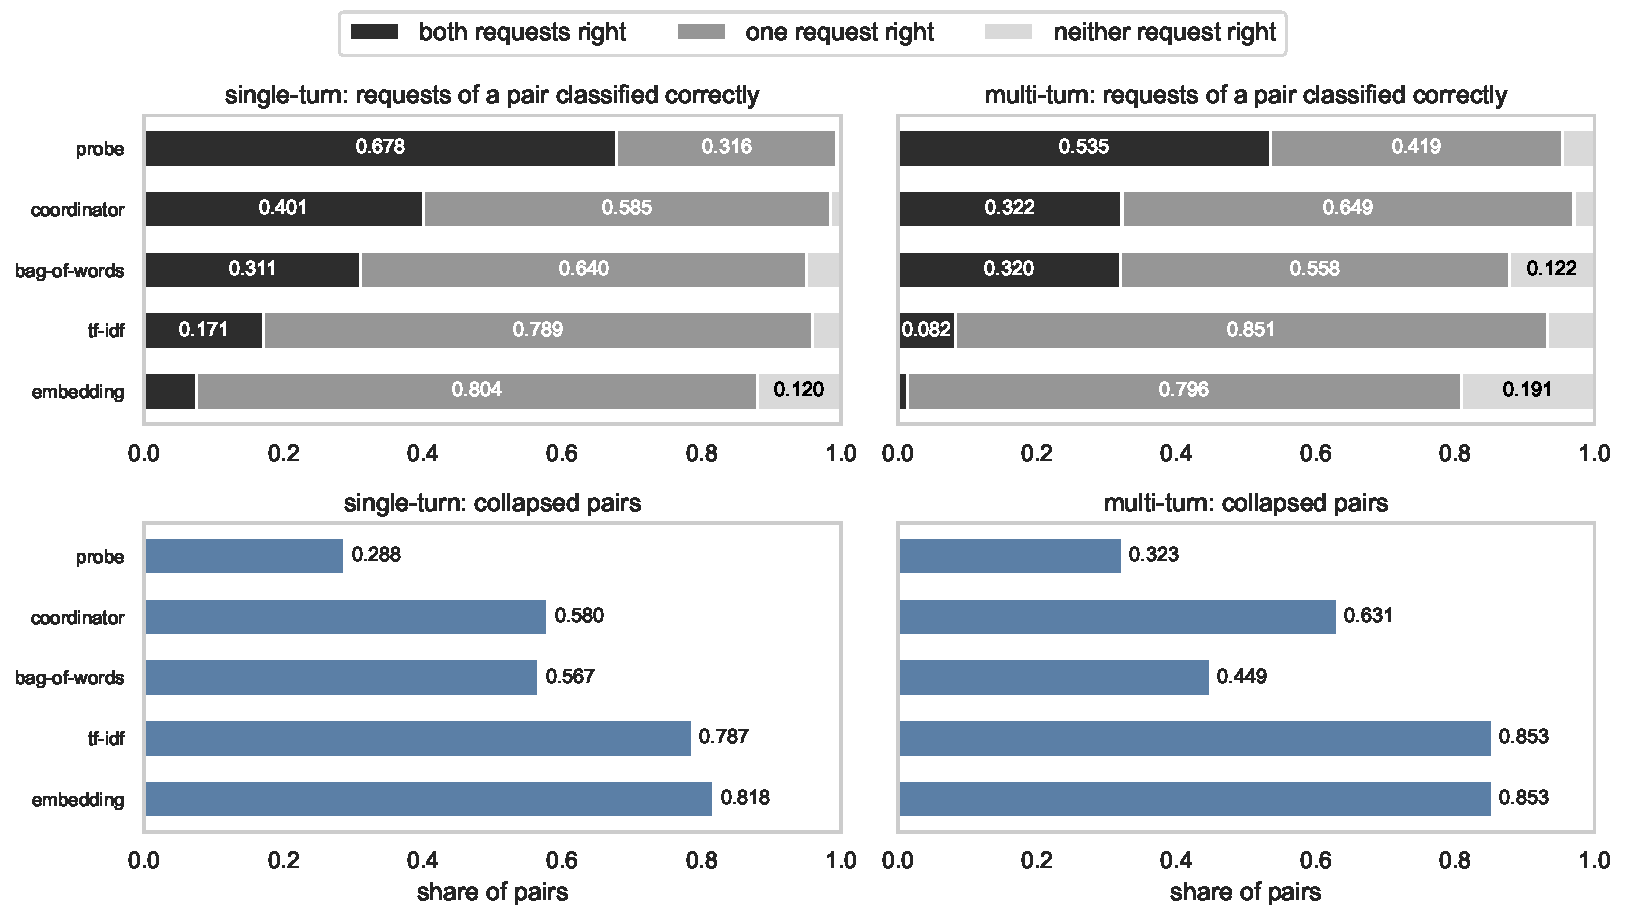
\includegraphics[width=\textwidth]{images/plots/overview/overview_pairs.pdf}
    \caption[Adversarial pair correctness and collapsed pairs per classifier]{Top: share of the 450 \texttt{adversarial} pairs in which each classifier classifies both, one or neither of the two requests correctly. Bottom: share of collapsed pairs. Single-turn dataset on the left, multi-turn dataset on the right. The probe and the coordinator values are the mean of the seven runs on the same dataset. The text-only classifiers do not depend on the model.}
    \label{fig:ch8-pairs}
\end{figure}

The probe collapses fewer pairs than the coordinator on both datasets, with a mean share of collapsed pairs of 0.288 and 0.323 against 0.580 and 0.631. The coordinator collapses fewer pairs than the TF-IDF and embedding classifiers, but more than the bag-of-words classifier, which has a share of collapsed pairs of 0.567 and 0.449. The probe also has the highest share of pairs with both requests right on both datasets, with a mean of 0.678 and 0.535 against 0.401 and 0.322 for the coordinator.

\FloatBarrier

\subsection{Decoy Predictions}
\label{subsec:ch8-failure-decoy}

On \texttt{natural} and \texttt{adversarial}, every request states a waived constraint, and the sub-agent that owns it is the decoy (Section~\ref{subsec:constraints-binding-waived}). The decoy predictions are used to observe how often each classifier is misled by the waived constraint, and whether the probe is misled less often than the coordinator and the text-only classifiers. The \emph{decoy rate} of a classifier is defined as the share of the samples of a tier on which the classifier predicts the decoy. Figure~\ref{fig:ch8-decoy} reports the decoy rate of every classifier.

\begin{figure}[htbp]
    \centering
    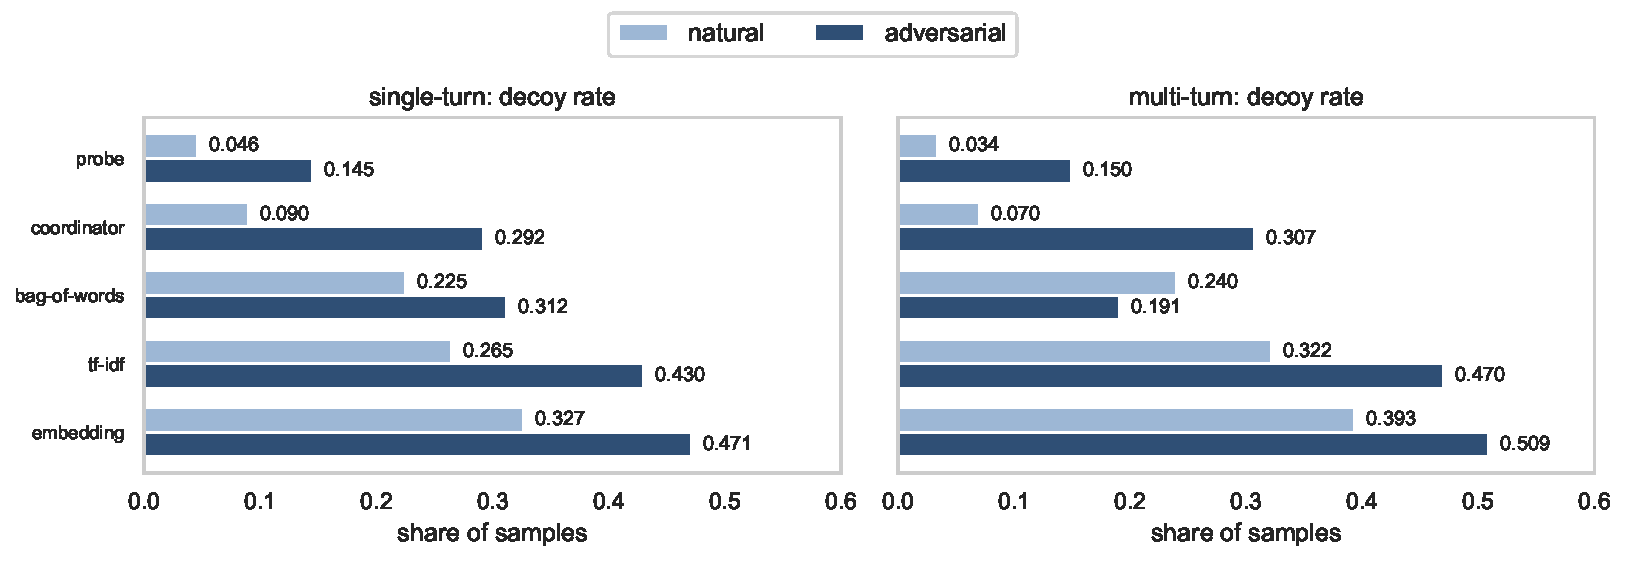
\includegraphics[width=\textwidth]{images/plots/overview/overview_decoy.pdf}
    \caption[Decoy rate by tier, single-turn and multi-turn datasets]{Decoy rate: share of the samples of each tier on which each classifier predicts the decoy, single-turn dataset on the left and multi-turn dataset on the right. The probe and the coordinator values are the mean of the seven runs on the same dataset. The text-only classifiers do not depend on the model.}
    \label{fig:ch8-decoy}
\end{figure}

The probe has the lowest mean decoy rate on both tiers and both datasets. The coordinator has the second lowest, except on the multi-turn \texttt{adversarial} tier, where the bag-of-words classifier has the second lowest.

The probe improves on the coordinator in the three measures of this section: on both datasets it has a lower mean share of collapsed pairs, a higher mean share of pairs with both requests right, and a lower mean decoy rate on both tiers. The correct sub-agent is therefore encoded in the hidden states of the coordinator, but the coordinator does not select it as accurately as the probe. This may come from the training of the probe, which learns to read the sub-agent from the hidden states on labeled samples of the dataset, while the coordinator chooses according to the routing policy stated in its prompt.

\subsection{Answer to RQ2}
\label{subsec:ch8-rq2-answer}

\phantomsection\label{rq:ch8-rq2}
\begin{rqbox}[RQ2]
Does a probe on the coordinator's hidden states recover the correct sub-agent more accurately than classifiers trained on a fixed representation of the query text, such as raw word counts, TF-IDF weighting, or sentence embeddings?
\end{rqbox}


\noindent Yes. Section~\ref{sec:ch7-observations} reports that the probe is more accurate than all three text-only classifiers on the \texttt{natural} and the \texttt{adversarial} tier of both datasets.

On the \texttt{adversarial} pairs, the probe has the lowest mean share of collapsed pairs and the highest mean share of pairs with both requests right on both datasets, and it has the lowest mean decoy rate on both tiers and both datasets. The binding constraint stated in a request can therefore be read more accurately from the hidden state at the last prompt token than from the representations of the request text that the text-only classifiers use.

The advantage is partial, because the errors of the probe partly follow the errors of the text-only classifiers: $a_p^{-}$ is lower than $a_p^{+}$ in every comparison of Table~\ref{tab:ch8-dependence}, with $\kappa_n$ between 0.151 and 0.424.

\FloatBarrier


\section{Relative Depth of the Optimal Layer}
\label{sec:ch8-depth}

\phantomsection\label{rq:ch8-rq3-intro}
\begin{rqbox}[RQ3]
Does the optimal probe layer fall at a consistent relative depth across different LLMs?
\end{rqbox}


\noindent To answer \hyperref[rq:ch8-rq3-intro]{\textbf{RQ3}}, this section measures where the optimal layer of each run falls in the stack of layers of its model (Section~\ref{subsec:block}), expressed as a fraction of the number of layers, called the \emph{relative depth}. Section~\ref{sec:ch7-results} reports the optimal layer of each run, the layer at which the probe reaches its highest accuracy. That layer index does not compare directly across models, because the layer count in the pool ranges from 30 to 80, so a specific layer does not mark the same depth in every model. A relative depth that is similar across the models indicates that the routing signal concentrates at the same relative depth in every model.

\subsection{Relative Depth of the Optimal Layer per Run}
\label{subsec:ch8-depth-values}

Each optimal layer is divided by the last layer index, which places it in $[0, 1]$ and gives its relative depth. This rescaling makes the positions comparable across models. Figure~\ref{fig:ch8-depth} plots the relative depth of the optimal layer for the fourteen runs.

\begin{figure}[htbp]
    \centering
    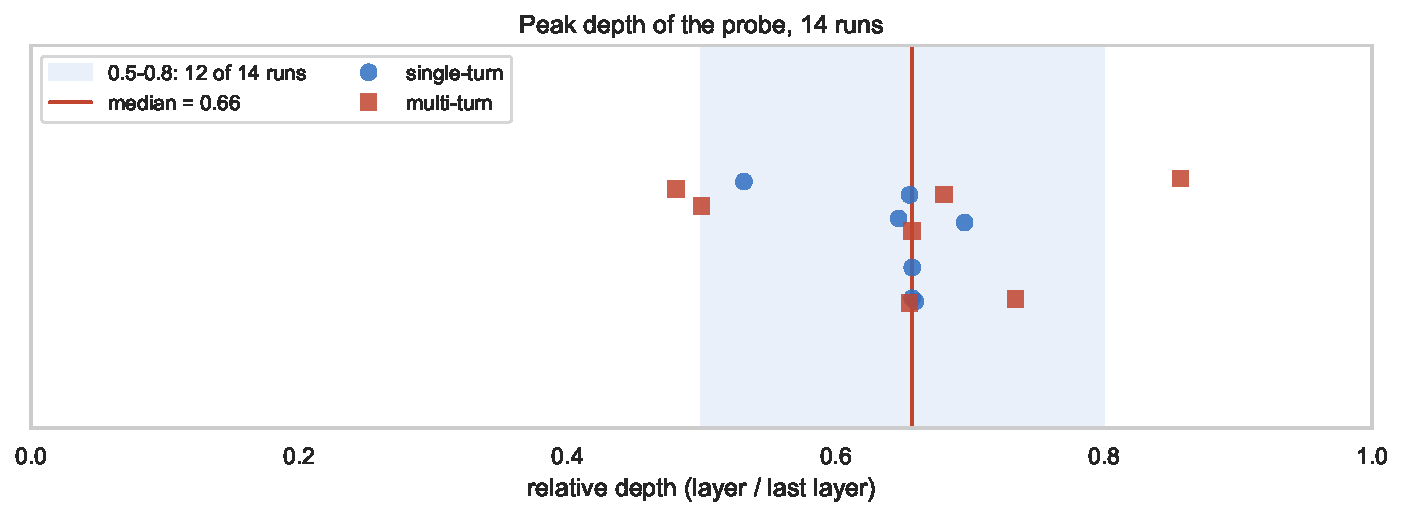
\includegraphics[width=\textwidth]{images/plots/overview/overview_depth.pdf}
    \caption[Relative depth of the probe's optimal layer]{Relative depth of the probe's optimal layer, fourteen runs.}
    \label{fig:ch8-depth}
\end{figure}

The median relative depth is 0.66, with quartiles at 0.65 and 0.68. Twelve of the fourteen runs fall between 0.5 and 0.8. The two remaining runs fall outside that range: Llama 3.3 70B multi-turn at 0.48, 0.02 below the lower bound, and Qwen3 8B multi-turn at 0.86, 0.06 above the upper bound. The single-turn and the multi-turn runs give the same median, so the number of turns does not move the relative depth of the optimal layer, but the two groups differ in spread: the standard deviation of the relative depth is 0.05 for the single-turn runs and 0.13 for the multi-turn runs. Section~\ref{subsec:ch8-multi-turn} relates the larger multi-turn drop in probe accuracy to a less separable representation of the sub-agents in the multi-turn hidden states, and the same reduced separability could also explain why the multi-turn relative depth is less consistent across models.

Ratnakar et al. note that deeper layers dominate in typical probing results, but their own LatentGate results differ: the optimal layer falls at a relative depth of 0.25 to 0.50 \cite{ratnakarLatentGateLowLatencySemantic2026}. They give as a likely reason that their agent-routing task requires broad topic discrimination rather than fine-grained linguistic analysis. The median relative depth of 0.66 here is larger, so the optimal layer falls in the second half of the layer stack. The routing task in this work requires deciding which of several constraints binds on a shared scenario, a finer-grained judgment than topic-level agent selection. Following the explanation of Ratnakar et al., this finer-grained judgment may be the reason why the optimal layer falls deeper than in LatentGate.

\subsection{Answer to RQ3}
\label{subsec:ch8-rq3-answer}

\phantomsection\label{rq:ch8-rq3}
\begin{rqbox}[RQ3]
Does the optimal probe layer fall at a consistent relative depth across different LLMs?
\end{rqbox}


\noindent Yes. The relative depth of the optimal layer lies between 0.5 and 0.8 in twelve of the fourteen runs, with a median of 0.66 that is the same on the single-turn and on the multi-turn dataset.

The consistency is lower in the multi-turn setting. Both runs outside the 0.5 to 0.8 band are multi-turn, Llama 3.3 70B at 0.48 and Qwen3 8B at 0.86, and the standard deviation of the relative depth is 0.13 on the multi-turn dataset against 0.05 on the single-turn dataset.

The claim that the optimal layer occurs at a consistent relative depth is limited to the pool of models analyzed in this work, which is too small to provide a valid generalization.

\FloatBarrier


\section{The Probe as an Evaluation Flag}
\label{sec:ch8-error-flag}

\phantomsection\label{rq:ch8-rq4-intro}
\begin{rqbox}[RQ4]
Can the disagreement between the probe and the coordinator be used as a runtime flag for likely misrouting?
\end{rqbox}


\noindent To answer \hyperref[rq:ch8-rq4-intro]{\textbf{RQ4}}, the probe is measured as a flag for a likely misroute. Section~\ref{sec:ch8-overview} shows that the probe is more accurate than the coordinator on the whole dataset, in all the runs. When the probe and the coordinator predict a different sub-agent for the same request, at most one of them is right, and the coordinator is the more likely one to be wrong, because it is the less accurate of the two. The \emph{disagreement flag} is raised on a sample when the out-of-fold prediction of the probe differs from the sub-agent predicted by the coordinator. The flag is measured against the error rate of the coordinator, to determine whether it marks the misroutes more often than the base rate and how many correct decisions it marks by mistake.

\subsection{Metrics}
\label{subsec:ch8-error-flag-metrics}

Four metrics are used to measure the quality of the disagreement flag. Each metric treats an error of the coordinator as the positive class and a raised flag as a positive prediction:

\begin{itemize}
    \item \textbf{precision}: the share of the flagged samples where the coordinator is wrong,
    \[
        P(\text{coordinator wrong} \mid \text{flagged})
    \]
    \item \textbf{recall}: the share of the coordinator's errors that are flagged,
    \[
        P(\text{flagged} \mid \text{coordinator wrong})
    \]
    \item \textbf{F1-score}: the harmonic mean of precision and recall, a single value for how well the flag covers the coordinator's errors,
    \[
        2 \cdot \frac{\text{precision} \cdot \text{recall}}{\text{precision} + \text{recall}}
    \]
    \item \textbf{false positive rate} (FPR): the share of the coordinator's correct decisions that are flagged, the same metric that Section~\ref{subsec:ch7-metrics} uses for the ROC curve,
    \[
        P(\text{flagged} \mid \text{coordinator right})
    \]
\end{itemize}

The \emph{base error rate} is the share of the samples of a run where the coordinator predicts the wrong sub-agent, and it varies from 0.112 to 0.298 across the runs. A low base error rate leaves few errors for the flag to hit, which lowers precision and the F1-score. Precision and the F1-score must therefore be read against the base error rate of their own run, reported next to them. The F1-score measures the quality of the flag on one run. A model with a high base error rate gives the flag more errors to find, so it can reach a higher F1-score while its coordinator routes less accurately.

The F1-score is computed from precision and recall only, so it does not count the correct decisions of the coordinator that the flag leaves unmarked. The false positive rate measures the share of the correct decisions that are flagged by the probe.

\subsection{Results}
\label{subsec:ch8-error-flag-results}

Table~\ref{tab:ch8-error-flag} reports the four metrics of each run, together with the base error rate of the coordinator and the margin $\Delta$ of Table~\ref{tab:ch8-overview}.

The precision of the flag (the share of the flagged samples where the coordinator is wrong) is between 0.598 and 0.826. In each of the fourteen runs it exceeds the base error rate of the coordinator in that same run, which is between 0.112 and 0.298. The recall (the share of the errors of the coordinator that are flagged) is between 0.540 and 0.797. The false positive rate is between 0.028 and 0.160, and below 0.100 in twelve of the runs. The F1-score, which combines precision and recall, is between 0.601 and 0.811.

The flag is less reliable on the multi-turn dataset. Its false positive rate rises for six of the seven models, by between 0.015 and 0.068, and is unchanged for Qwen2.5 72B. The probe loses more accuracy than the coordinator in the multi-turn setting (Section~\ref{subsec:ch8-multi-turn}), and a probe with lower accuracy raises the flag on more of the correct decisions of the coordinator.

\begin{table}[H]
    \centering
    \small
    \begin{tabular}{@{}lcccccc@{}}
        \toprule
        \textbf{Model} & \textbf{Precision} & \textbf{Recall} & \textbf{F1-score} & \textbf{Base error} & \textbf{FPR} & $\boldsymbol{\Delta}$ \\
        \midrule
        \multicolumn{7}{@{}l}{\textit{Single-turn}} \\
        \midrule
        \texttt{gemma4-e2b-it}     & 0.738 & 0.700 & 0.718 & 0.264 & 0.089 & 0.112 \\
        \texttt{qwen3-4b}          & 0.756 & 0.717 & 0.736 & 0.248 & 0.077 & 0.112 \\
        \texttt{qwen3-8b}          & 0.683 & 0.670 & 0.677 & 0.228 & \worst{0.092} & 0.073 \\
        \texttt{gemma4-12b-it}     & 0.741 & 0.560 & \worst{0.638} & 0.127 & \best{0.028} & 0.043 \\
        \texttt{gemma4-26b-a4b-it} & 0.681 & 0.600 & \worst{0.638} & 0.112 & 0.035 & 0.033 \\
        \texttt{llama3.3-70b}      & 0.779 & 0.763 & 0.771 & 0.230 & 0.065 & 0.124 \\
        \texttt{qwen2.5-72b}       & 0.826 & 0.797 & \best{0.811} & 0.239 & 0.053 & 0.146 \\
        \midrule
        \multicolumn{7}{@{}l}{\textit{Multi-turn}} \\
        \midrule
        \texttt{gemma4-e2b-it}     & 0.712 & 0.778 & 0.744 & 0.298 & 0.134 & 0.080 \\
        \texttt{qwen3-4b}          & 0.703 & 0.688 & 0.696 & 0.255 & 0.099 & 0.069 \\
        \texttt{qwen3-8b}          & 0.598 & 0.671 & 0.632 & 0.262 & \worst{0.160} & 0.006 \\
        \texttt{gemma4-12b-it}     & 0.679 & 0.540 & \worst{0.601} & 0.145 & \best{0.043} & 0.024 \\
        \texttt{gemma4-26b-a4b-it} & 0.673 & 0.639 & 0.655 & 0.144 & 0.052 & 0.022 \\
        \texttt{llama3.3-70b}      & 0.736 & 0.653 & 0.692 & 0.264 & 0.084 & 0.074 \\
        \texttt{qwen2.5-72b}       & 0.805 & 0.725 & \best{0.763} & 0.232 & 0.053 & 0.107 \\
        \bottomrule
    \end{tabular}
    \caption[Probe read as a flag on the coordinator's decision]{The probe read as a flag on the coordinator's decision: precision, recall, the F1-score, the coordinator's base error rate, the false positive rate (FPR), and the margin $\Delta$ of Table~\ref{tab:ch8-overview}. In each dataset, the best F1-score and FPR are in bold and the worst are underlined.}
    \label{tab:ch8-error-flag}
\end{table}

\FloatBarrier

\subsection{Answer to RQ4}
\label{subsec:ch8-rq4-answer}

\phantomsection\label{rq:ch8-rq4}
\begin{rqbox}[RQ4]
Can the disagreement between the probe and the coordinator be used as a runtime flag for likely misrouting?
\end{rqbox}


\noindent Yes. For every model, on both datasets, the precision of the flag is between 0.598 and 0.826 and above the base error rate of that model, which is between 0.112 and 0.298. The recall is between 0.540 and 0.797, and the false positive rate is between 0.028 and 0.160, below 0.100 in twelve of the fourteen runs.

The flag is less reliable in the multi-turn setting, where its false positive rate rises for six of the seven models, by between 0.015 and 0.068.

\FloatBarrier


\flushbottom

\chapter{Conclusions}
\label{chap:conclusions}

This chapter discusses what the answers to the research questions imply for the development of coor\-di\-na\-tor-based multi-agent systems: how much a probe on the hidden states of the coordinator adds to the routing decision, and how it can be used as a misrouting flag. It then describes the conditions under which a multi-agent system can use such a probe, which concern whether the inference service that runs the coordinator returns its hidden states together with the response, the cost of extracting them, and the labeled data needed to train the probe. Next, the chapter states the limitations of the study, which arise from the synthetic dataset, the structure of the multi-turn conversations, the model pool, and the position from which the probe reads the hidden states. Finally, the chapter outlines directions for future work and closes with the conclusions drawn from the findings of this work.

\section{Implications}
\label{sec:ch9-implications}

The answer to \hyperref[rq:ch8-rq1]{\textbf{RQ1}} in Section~\ref{subsec:ch8-rq1-answer} shows that a probe on the hidden states of a coordinator selects the correct sub-agent more reliably than the coordinator itself. The probe is a linear classifier on the hidden state at the last prompt token, which the coordinator already computes, so a multi-agent system obtains a more accurate routing decision without an additional model call. The gain grows as the correct sub-agent becomes more difficult to determine from the wording of the request, which is where the coordinator misroutes most often. The gain is also smaller when the request is part of a multi-turn conversation.

The answer to \hyperref[rq:ch8-rq2]{\textbf{RQ2}} in Section~\ref{subsec:ch8-rq2-answer} shows that the same gain is not obtained by the three text-only classifiers of this work, which are logistic regressions trained on a bag-of-words, a TF-IDF and an embedding representation of the request text and need no access to the hidden states. As the correct sub-agent becomes more difficult to determine from the wording of the request, the accuracy of each text-only classifier falls more than the accuracy of the probe. On these requests, the hidden states of the coordinator therefore carry routing information that the representations of the request text do not provide, and this information is what justifies reading the hidden states. As the difficulty of the requests increases, the probe is the classifier that retains the most accuracy to evaluate the routing decision of the coordinator.

The answer to \hyperref[rq:ch8-rq3]{\textbf{RQ3}} in Section~\ref{subsec:ch8-rq3-answer} shows that the optimal layer for the probe falls at a consistent relative depth across the models of this work. For a new coordinator model, it is therefore likely to fall at a similar depth, and the layer sweep aimed at finding it can be restricted around that depth.

Because the probe is more accurate than the coordinator, it can be used as an evaluation flag on the routing decision of the coordinator. The answer to \hyperref[rq:ch8-rq4]{\textbf{RQ4}} in Section~\ref{subsec:ch8-rq4-answer} shows that the disagreement flag, raised when the probe and the coordinator select different sub-agents, marks the requests that the coordinator is likely to misroute, with a precision above the base error rate of the coordinator in every run. When the flag is raised, the execution of the request can be stopped (Section~\ref{sec:early-exit-feedback-loop}), or the request can be kept for later review by a human. On the single-turn dataset, the flag is raised on between 56.0\% and 79.7\% of the misroutes of the coordinator, depending on the model, and between 68.1\% and 82.6\% of the flagged requests are misroutes of the coordinator. On the multi-turn dataset, the flag is raised on between 54.0\% and 77.8\% of the misroutes, and between 59.8\% and 80.5\% of the flagged requests are misroutes of the coordinator.

Because the probe is more accurate than the coordinator, the request could also be handed off to the sub-agent that the probe predicts, instead of the sub-agent that the coordinator selects. The probe would then replace the routing decision of the coordinator, instead of serving as an evaluation flag on it. With this replacement, a smaller coordinator can give a more accurate routing decision than a larger one: on both datasets, the probes on Qwen3 4B Instruct 2507 and on Gemma 4 E2B IT are more accurate than the Llama 3.3 70B Instruct and the Qwen2.5 72B Instruct coordinators (Tables~\ref{tab:ch7-qwen3-4b}, \ref{tab:ch7-gemma4-e2b-it}, \ref{tab:ch7-llama33-70b} and~\ref{tab:ch7-qwen25-72b}). Ratnakar et al. reach the same conclusion with LatentGate, where a linear probe on the hidden states of Qwen2.5 1.5B Instruct routes queries more accurately than prompt-based routers built on GPT-4.1, GPT-4.1-nano and Gemini 2.5 Flash \cite{ratnakarLatentGateLowLatencySemantic2026}. However, this replacement may not be possible when the coordinator has responsibilities other than routing, such as conducting the conversation with the user, producing the final response from the response of the selected sub-agent (Section~\ref{sec:coordinator}), or applying guardrails (Section~\ref{sec:security-evaluation}).


\section{Conditions of Use}
\label{sec:ch9-conditions}

The implications just described assume that the hidden states of the coordinator are available and that a probe has been trained on them. A multi-agent system meets this assumption only under certain conditions of use, which concern whether the inference server returns the hidden states of the coordinator, the memory needed to extract them, and the labeled data needed to train the probe.

LLM-based agents commonly interact with large language models through an \emph{inference server}, a process that loads a model and runs it each time it receives a request. The model runs on the GPUs of the machine that hosts the server, so the agent does not need to load the model weights or run the forward pass itself. The agent invokes the model through the API endpoints that the server exposes: it sends the prompt in a request and receives the generated text in the response. These endpoints can belong to a frontier-model API that a provider runs on its own infrastructure, such as the OpenAI API or the Anthropic API. They can also belong to a self-hosted inference server, deployed on self-managed infrastructure. Common self-hosted inference servers include \texttt{llama.cpp}, \texttt{vLLM}, \texttt{SGLang}, and \texttt{MLX}.

\subsection{Hidden States in the Server Response}
\label{subsec:ch9-flag-access}

Frontier-model APIs do not provide access to the hidden states. Exposing them may also be a security risk for the provider, because they allow a third party to reconstruct parts of a proprietary model without access to its weights. Carlini et al. showed that the log-probabilities and the logit bias exposed by production APIs were sufficient to recover the final projection layer and the hidden dimension of OpenAI models \cite{carliniStealingPartProduction2024}. The hidden states expose more of the model than these outputs. Jiao et al. used \emph{knowledge distillation} to train a smaller model that reproduces the hidden states of a larger model, so that the smaller model could be used in place of the larger one \cite{jiaoTinyBERTDistillingBERT2020}. A third party that receives the hidden states of a proprietary model could apply the same method to obtain a smaller model that replaces the proprietary one.

Self-hosted inference servers have no standard method to provide access to the hidden states. Each server that supports this access implements it in a different way. The documentation of \texttt{llama.cpp} and of \texttt{MLX} lists no option to return the hidden states \cite{LlamacppToolsServer, MlxlmMlx_lmSERVERmd}. The \texttt{vLLM} server can extract the hidden states of the prompt tokens at selected layers, but it does not return them to the caller: it writes them to a file on disk and returns only the path of the file in the response \cite{teamExtractingHiddenStates2026}. Among the four servers, only \texttt{SGLang} returns the hidden states in the response, through a server argument that enables this feature \cite{ServerArguments}.

\subsection{Inference Cost}
\label{subsec:ch9-flag-cost}

Where the hidden states are accessible, extracting them increases the memory that inference requires. As Section~\ref{subsec:hidden-states} describes, the hidden state $h^{(\ell)}_i$ of every layer $\ell$ and every token $i$ is a vector of $d_{\mathrm{model}}$ values. The extracted hidden states are held in VRAM or RAM, and the memory they occupy grows linearly with the number of layers and tokens they cover.

Each value of a hidden state vector occupies $b$ bytes, with $b = 2$ for 16-bit and $b = 4$ for 32-bit floating-point values. The hidden states of one token therefore occupy $b \times d_{\mathrm{model}}$ bytes at one layer and $b \times L \times d_{\mathrm{model}}$ bytes at all $L$ layers. Table~\ref{tab:ch9-hidden-state-size} reports both sizes for the models of Table~\ref{tab:model-properties}.

\begin{table}[htbp]
    \centering
    \small
    \begin{tabular}{lrrrrrr}
        \toprule
        & & & \multicolumn{2}{c}{One layer (KiB)} & \multicolumn{2}{c}{All $L$ layers (KiB)} \\
        \cmidrule(lr){4-5} \cmidrule(lr){6-7}
        Model & $d_{\mathrm{model}}$ & $L$ & 16-bit & 32-bit & 16-bit & 32-bit \\
        \midrule
        Gemma 4 E2B IT & 1536 & 35 & 3.0 & 6.0 & 105.0 & 210.0 \\
        Qwen3 4B Instruct 2507 & 2560 & 36 & 5.0 & 10.0 & 180.0 & 360.0 \\
        Qwen3 8B & 4096 & 36 & 8.0 & 16.0 & 288.0 & 576.0 \\
        Gemma 4 12B IT & 3840 & 48 & 7.5 & 15.0 & 360.0 & 720.0 \\
        GPT-OSS 20B & 2880 & 24 & 5.6 & 11.3 & 135.0 & 270.0 \\
        Gemma 4 26B A4B IT & 2816 & 30 & 5.5 & 11.0 & 165.0 & 330.0 \\
        Llama 3.3 70B Instruct & 8192 & 80 & 16.0 & 32.0 & 1280.0 & 2560.0 \\
        Qwen2.5 72B Instruct & 8192 & 80 & 16.0 & 32.0 & 1280.0 & 2560.0 \\
        \bottomrule
    \end{tabular}
    \caption[Hidden-state memory per token, at one layer and at all $L$ layers]{Memory occupied by the hidden states of one token, at one layer and at all $L$ layers, with 16-bit and 32-bit floating-point values (1~KiB = 1024 bytes).}
    \label{tab:ch9-hidden-state-size}
\end{table}

Requesting the hidden states together with the response from an inference server may therefore increase the memory usage of the server and slow down inference. It may also considerably increase the size of the payload that the server returns for each request.

\subsection{Cold-Start Problem}
\label{subsec:ch9-flag-cold-start}

A probe is subject to a \emph{cold-start problem}, because it needs labeled data to be trained. Every probe in this work is trained on samples whose correct sub-agent is set by the generation plan of Chapter~\ref{chap:dataset-construction}. A real production system typically has no labeled data at the time of its first release. Labeled data accumulates only after the system is deployed, either from human annotation or from usage history annotated after the routing decision. Once enough labeled data has accumulated, a probe can be trained and used as a misrouting flag. However, the probe would need to be retrained every time the routing task changes, for example when a sub-agent is added, removed, or redefined. It would also need to be retrained every time the coordinator model changes, because a different model may have a different optimal layer, and the accuracy gained by probing that layer may also differ. A change of the coordinator prompt may also affect the accuracy of the probe, because the hidden state at the last prompt token is computed from the entire prompt. The effect of a prompt change on the accuracy of the probe is not measured in this work, and neither is the number of labeled samples a probe needs before it can be used as a misrouting flag. Section~\ref{sec:ch9-future-work} lists both questions as future work.


\section{Limitations of the Study}
\label{sec:ch9-limitations-work}

The implications that Section~\ref{sec:ch9-implications} draws from the results of Chapter~\ref{chap:results-analysis} are subject to the limitations stated in this section, which concern the synthetic dataset, the structure of the multi-turn conversations, the scale and composition of the model pool, and the position from which the probe reads the hidden states.

\subsection{Synthetic Dataset}
\label{subsec:ch9-limitations-dataset}

Every result reported in this work is measured on the single-turn and multi-turn datasets described in Chapter~\ref{chap:dataset-construction}. Both datasets are generated synthetically by prompting a large language model, and each sample is built to meet the requirements stated in Section~\ref{sec:dataset-requirements}. The content and the distribution of the requests are therefore determined by the design of the generation pipeline. Every accuracy in this work is measured on this distribution. The requests that a deployed multi-agent system receives from its users may follow a different distribution. The accuracy gain of the probe over the coordinator in such a system may therefore be larger or smaller than the one measured in Chapter~\ref{chap:results-analysis}.

No human annotation is performed on the datasets. The label of each sample comes from the generation plan, and it is validated only by the automated audit stage. As Section~\ref{subsec:pipeline-audit-repair} describes, this stage applies deterministic structural rules, the Jaccard index on \texttt{adversarial} pairs, and the verdict of an LLM oracle. A manual revision is applied only to the samples that the oracle check flags, so every other sample keeps the label assigned by the plan without human verification. Some of these samples may therefore be mislabeled, which would affect every accuracy reported in Chapter~\ref{chap:results-analysis}.

\subsection{Structure of the Multi-Turn Conversations}
\label{subsec:ch9-limitations-multiturn}

The generation pipeline builds every multi-turn sample with the same structure. As Section~\ref{subsec:multiturn-derivation} describes, each conversation contains five messages, which alternate between the developer and the coordinator. In the \texttt{adversarial} tier, the two members of a pair share the first four messages, so that they differ only in the final message.

A conversation between a developer and a coordinator may span tens or hundreds of turns. Its topic may change between turns, and messages unrelated to the routing decision may be interleaved with the messages that carry the information needed for routing.

On the multi-turn dataset, the probe loses more accuracy than the coordinator in all seven models, as Section~\ref{subsec:ch8-multi-turn} reports. Because every conversation has the same structure and the same number of turns, this drop is observed only on conversations of this form, and the dataset does not allow an analysis of how the probe behaves on conversations of different lengths and structures. It is therefore unknown whether the probe remains more accurate than the coordinator on such conversations, and whether the disagreement flag can still mark the misroutes of the coordinator.

\subsection{Scale and Composition of the Model Pool}
\label{subsec:ch9-limitations-scale}

As Section~\ref{sec:model-choice} describes, every model in the pool is an open-weight model with at most 72 billion parameters. The model pool is therefore limited to this parameter count, and the results of this work apply only to models up to this size.

The model pool is also limited in composition, because its models are not distributed evenly across families and sizes. Of the seven models analyzed in Chapter~\ref{chap:results-analysis}, three belong to the Gemma 4 family and two to the Qwen3 family, and all five have at most 26 billion parameters. Llama 3.3 70B and Qwen2.5 72B are the only two models above that size, and each is the only model of its family in the pool. The results are consistent across the four families, but they are derived mostly from models of the Gemma 4 and Qwen3 families, so they do not show whether the accuracy gain of the probe over the coordinator depends on the model family.

\subsection{Probe Input Position}
\label{subsec:ch9-limitations-extraction}

As Section~\ref{subsec:probe-position-requirements} states, every probe in this work reads the hidden state at the last prompt token. The only exception is GPT-OSS 20B, whose hidden state at the last reasoning token is also probed for comparison in Section~\ref{sec:ch8-gpt-oss}. The last prompt token is chosen because of masked attention: as Section~\ref{subsec:last-token} describes, it is the only position whose hidden state is computed from the entire prompt.

The position from which the hidden states are read may affect the accuracy of a probe. For GPT-OSS 20B, neither the last prompt token nor the last reasoning token gives a probe that improves on the coordinator, so the position must be chosen according to the model architecture. For example, Healy et al. reported that detection accuracy varies with the method used to extract hidden states from a query \cite{healyInternalRepresentationsIndicators2026}. LatentGate is one example of a different choice, because it pools the hidden states over every token of the query instead of reading a single position \cite{ratnakarLatentGateLowLatencySemantic2026}. Since every probe in this work is trained only on the hidden state at the last prompt token, the results do not allow a comparison between different probing positions.


\section{Future Work}
\label{sec:ch9-future-work}

\paragraph{Validation against production data.} On the datasets of this work, the probe is more accurate than the coordinator in seven of the eight models, and its disagreement with the coordinator marks coordinator errors, as Section~\ref{subsec:ch8-rq4-answer} states. Every sample of these datasets is generated from a fixed taxonomy of five sub-agents and follows the patterns defined by the generation plan. Requests collected from a coordinator-based multi-agent system in use may not follow a predefined set of patterns, and they may be incomplete, ambiguous, or unrelated to any sub-agent. A labeled dataset of such requests would measure the accuracy of the probe under this variability, and this accuracy would determine how useful the probe is as a misrouting flag in a multi-agent system in use.

A multi-agent system in use may already have a set of production requests annotated with the correct sub-agent, which is used to evaluate the routing decision of its coordinator. Future work could validate the probe on such a system with the following procedure:

\begin{enumerate}
    \item \textbf{Training.} The hidden states of the coordinator are collected by running each annotated request through the prefill step (Section~\ref{subsec:prefill-decode}) of the model in use, with no response token generated. A probe is trained on these hidden states with $k$-fold cross-validation, as for the probes of Section~\ref{subsec:ch7-probe}.
    \item \textbf{Deployment.} The probe is deployed next to the coordinator, on an inference server that returns the hidden states (Section~\ref{subsec:ch9-flag-access}), and it raises the disagreement flag on the incoming requests.
    \item \textbf{Collection period.} The flagged requests are collected for a defined period of time.
    \item \textbf{Annotation.} At the end of the collection period, human annotators examine every flagged request and determine whether the coordinator misrouted it or the flag is a false positive.
\end{enumerate}

The fraction of the flagged requests that are misrouted gives the precision of the flag in real usage. This precision would show how effective a probe trained on evaluation data is as a misrouting flag on the requests of a multi-agent system in use.

\paragraph{Adaptation to a changing sub-agent set.} The sub-agent set of a multi-agent system in use may change over time, for example when a new sub-agent is added or when the responsibilities of an existing one are redefined. Section~\ref{subsec:ch9-flag-cold-start} notes that a probe needs retraining after each of these changes. The labeled data collected before the change may no longer match the new routing task, so the probe could not be used as a misrouting flag until enough new labeled data has accumulated. A change of the sub-agent set also modifies the prompt of the coordinator, because every sub-agent is declared in the prompt as a tool (Section~\ref{subsec:ch7-coordinator-prompt}). The hidden state at the last prompt token is computed from the entire prompt, so it may change even for requests whose correct sub-agent stays the same. The hidden states may also change when the prompt of the coordinator is modified and the sub-agent set stays the same.

Future work could study how the accuracy of an existing probe varies after each type of change: the addition, the removal, and the redefinition of a sub-agent. This study would show which changes leave the accuracy of the probe unaffected and which ones require new labeled data. Future work could also study whether an existing probe can be adapted to the new sub-agent set by reusing what it has already learned, for example by updating it with only the samples labeled after the change. If the adapted probe needs fewer labeled samples than a new probe to reach the same accuracy, fewer requests would need to be labeled after each change before the probe can be used again as a misrouting flag.

\paragraph{Detailed analysis of multi-turn behavior.} On the multi-turn dataset, the multi-turn drop of the probe is larger than the multi-turn drop of the coordinator in all seven models, as Section~\ref{subsec:ch8-multi-turn} reports. Section~\ref{subsec:ch9-limitations-multiturn} states that every conversation in this dataset has the same structure and the same number of messages. A conversation in a multi-agent system in use may span many more turns, change topic, and include turns unrelated to the routing decision. The hidden state at the last prompt token is computed from the entire conversation, so the information needed for routing may be spread across more turns or placed far from the last prompt token. The accuracy of the probe on such conversations may therefore differ from the one measured on the multi-turn dataset of this work.

Future work could build a synthetic multi-turn dataset in which the number of turns and the structure of the conversation vary as design factors. The structure could follow a defined taxonomy of patterns, such as topic drift, turns unrelated to the routing decision, and different positions of the turn that carries the routing information. Such a dataset would allow a study of how the accuracy of the probe varies across the patterns, and across shorter and longer conversations. The same dataset could also be used to test whether a probe that reads the hidden states at several positions, such as the last token of each turn, is more accurate on long conversations, or on conversations with topic drift, than a probe that reads only the last prompt token. The results would show whether the probe remains usable as a misrouting flag on conversations longer and less regular than the ones of this work.


\section{Final Remarks}
\label{sec:ch9-conclusion}

On requests whose correct sub-agent is difficult to determine from their wording, a linear probe on the hidden state at the last prompt token selects the correct sub-agent more often than the coordinator in seven of the eight models, and more often than the text-only classifiers. Its margin over the coordinator is largest on the requests that the coordinator misroutes most often. The hidden states of a coordinator therefore carry routing information that its stated decision does not reflect and that the wording of the request does not provide. The exception is GPT-OSS 20B, which reasons before it selects a sub-agent. Its last prompt token comes before the point where the routing decision may be formed, so the probing position must be chosen according to the model architecture.

On multi-turn conversations, the probe loses more accuracy than the coordinator in all seven models, so its margin is smaller. The routing information at the last prompt token may therefore be weaker when the request is spread over several turns.

The disagreement between the probe and the coordinator marks the requests that the coordinator is likely to misroute, with a precision above the base error rate of the coordinator in all fourteen runs, although it raises more false positives on multi-turn conversations. When the hidden states of the coordinator are accessible, a flagged request can be stopped or held for human review before it affects the rest of the run.

These results indicate that a linear probe on the hidden states of a coordinator can provide an evaluation signal on its routing decision. Such a probe may support failure attribution and improve the quality of coordinator-based multi-agent systems, because it identifies likely routing failures before they propagate through the rest of the multi-agent trace.




\appendix

\part{Appendices}

\chapter{Prompts}
\label{chap:appendix-prompts}

This appendix reports the prompt templates used by the dataset generation pipeline described in Section~\ref{sec:dataset-overview}, and the coordinator system prompt used in the probing setup of Chapter~\ref{chap:probing-results}.

\section{Sub-Agents and Collisions}
\label{sec:appendix-taxonomy}

\texttt{\$\{experts\}} and \texttt{\$\{collisions\}} recur across several templates and stay fixed for the whole dataset. \texttt{\$\{experts\}} lists the five sub-agents defined in Section~\ref{sec:dataset-overview} and what each one handles.

\begin{promptverbatim}
- time_to_market (Time-to-Market): Absolute time-to-market. Accepts hardcoding, skipped abstractions and technical debt to get something demonstrable now.
- scale_arch (Scalable Architecture): Future concurrency and horizontal growth. Decouples components, removes shared state, designs for many times the current load.
- resource_opt (Resource Optimization): Hard CPU, memory or cost ceilings. Strips abstractions and takes low-level control to fit inside a fixed budget.
- legacy_compat (Legacy Compatibility): Strict backward compatibility. Bound by published API contracts, existing clients and outdated dependencies that cannot move.
- strict_compliance (Strict Compliance): Security, privacy and regulatory standards. Zero-trust data handling, auditability, and rules that cannot be traded away.
\end{promptverbatim}

\texttt{\$\{collisions\}} lists the ten sub-agent pairs that pull against each other, one per pair of sub-agents, and the tension between them.

\begin{promptverbatim}
- time_to_market vs scale_arch: get it working today vs. build it for many times this load
- time_to_market vs resource_opt: the fastest path to build vs. the cheapest path to run
- time_to_market vs legacy_compat: hack it in now vs. never break an existing contract
- time_to_market vs strict_compliance: bypass the boundary to ship vs. the boundary is not optional
- scale_arch vs resource_opt: spread the work across more machines vs. fit it on the machines you pay for
- scale_arch vs legacy_compat: reshape the topology vs. keep the published interface intact
- scale_arch vs strict_compliance: move and replicate data freely vs. data may not leave its boundary
- resource_opt vs legacy_compat: strip the abstraction out vs. the signature must not change
- resource_opt vs strict_compliance: cut the overhead vs. the overhead is a required control
- legacy_compat vs strict_compliance: preserve the old behaviour vs. the old behaviour is now disallowed
\end{promptverbatim}

\section{Fact Generation}

\texttt{\$\{scenario\}} is the seed scenario text; \texttt{\$\{experts\}} is the shared taxonomy listing from Section~\ref{sec:appendix-taxonomy}.

\subsection{System prompt}
\begin{promptverbatim}
You describe the operating constraints a software team works under, for a
research dataset about request routing. Five specialists look at the same
system and optimise for different constraints:

${experts}

Write plainly and concretely. No code, no markdown, no lists inside a value.
\end{promptverbatim}

\subsection{User prompt}
\begin{promptverbatim}
System under discussion:
${scenario}

Write five requirements on this system, one per specialist, in the order listed
below. Each is one or two sentences, phrased as an operational fact about this
team's situation, and each must name the party that imposes it (a named role,
team, customer, body or budget owner) and say what they require.

${experts}

All five must be simultaneously plausible for the same team on the same system:
a reader should accept that every one of them is true, and that the only open
question is which one that team is actually being held to right now.

All five must also carry the same enforcement weight. Each one has a real owner
who can insist on it, and each one is the kind of thing that owner could also
sign off on relaxing for a while. Do not write some of them as laws and others
as ambitions: no requirement may read as inherently more non-negotiable than
the others. Do not use the specialist ids or names, and do not describe the
requirements as competing.
\end{promptverbatim}

\section{Resolution Rule}
\label{sec:appendix-resolution-rule}

\texttt{\$\{resolution\_rule\}} states the rule defined in Section~\ref{sec:dataset-overview} that decides which sub-agent is correct.

\begin{promptverbatim}
Exactly one requirement in the text is BINDING: someone with authority over this
team - their org, a customer, a regulator, a budget owner - is holding them to it
right now, and it is not open for discussion. The correct expert is the one that
owns that requirement.

Every other requirement has been WAIVED: whoever owns it has explicitly relieved
this team of it for the moment - signed off on the current behaviour, granted an
exception, accepted the tradeoff, moved it to a later milestone. A waived
requirement can still be serious, can still be what the developer cares about
most, and can still take up most of the message.
\end{promptverbatim}

\section{Query Generation}
\label{sec:appendix-query-generation}

\subsection{System prompt}

\begin{promptverbatim}
You write realistic developer messages for a research dataset about request
routing. Each message goes to a coordinator that must forward it to exactly one
of five specialists. The specialists are not topic areas: they all look at the
same code and optimise for different systemic constraints.

## The specialists
${experts}

## Pairs that pull against each other
${collisions}

## How the correct specialist is decided
${resolution_rule}

## Unbreakable rules
1. Prose only: no code, backticks, markdown, lists, headings, logs, stack
   traces, pseudo-code, or emphasis markers.
2. Never name the experts or their ids, and never use the words "expert",
   "route", "constraint", "mandate", "preference". The developer describes
   their situation, they do not classify it.
3. Exactly one expert must be correct for the message.
4. Give every constraint the same space, specificity and urgency; only the
   resolution rule above may separate them.
5. The developer speaks in their own words about their own system: no neutral
   summary, no phrasing lifted from the notes you are given.
6. The developer words the letting-go of a requirement in their own idiom,
   never in the wording these instructions use for it: "signed off", "granted
   an exception" and "waived" and "green light" must not appear in the text. Teams
   say it in many ways: fine with it for now, off our plate this quarter,
   nobody is chasing us on it any more, that ship has sailed until the review.
\end{promptverbatim}

\subsection{Single-Turn Query Generation}
\label{sec:appendix-single-turn}

\texttt{\$\{persona\}} names the voice the message is written in, \texttt{\$\{fact\_gold\}} is the binding requirement, \texttt{\$\{fact\_decoy\}} is the waived requirement in the natural tier, \texttt{\$\{fact\_north\}} and \texttt{\$\{fact\_south\}} are the two requirements of an adversarial pair, \texttt{\$\{tension\}} names the collision between two requirements, and \texttt{\$\{pattern\}} names the decoy pattern defined in Section~\ref{subsec:difficulty-tiers}.

\subsubsection{Plain tier}
\begin{promptverbatim}
System under discussion:
${scenario}

Voice: ${persona}

Requirement this developer is being held to right now:
${fact_gold}

Write one message from this developer asking for help with this system. Only
this one requirement is in play; do not introduce any other pressure. The
requirement is live and current: something they are held to as they write,
never something that shaped a past decision. Three to six sentences.
\end{promptverbatim}

\subsubsection{Natural tier}
\begin{promptverbatim}
System under discussion:
${scenario}

Voice: ${persona}

Requirement this developer is being held to right now:
${fact_gold}

Requirement that has been waived: the party named in it has explicitly relieved
the team of it for the time being: signed off on the current behaviour,
granted an exception, or moved it to a later milestone. The developer may still
care about it a great deal.
${fact_decoy}

These two pull against each other: ${tension}.

Write one message from this developer asking for help. Both requirements must
be visible and given comparable space, and the text must say plainly, in the
developer's own words, that the second one has been waived and by whom. State
the live requirement as an ordinary fact of their situation, not as an
emphasised demand. The waived requirement keeps none of its binding force:
no hard ceiling, no date that still stands, no owner who will not budge.
Four to eight sentences.
\end{promptverbatim}

\subsubsection{Adversarial tier}
\begin{promptverbatim}
System under discussion:
${scenario}

Requirement NORTH:
${fact_north}

Requirement SOUTH:
${fact_south}

These pull against each other: ${tension}.

Shape of the message: ${pattern}

Voice: ${persona}

Write two versions of one developer message, four to eight sentences, describing
the situation in the shape above with both requirements in play. They are the
same text word for word, closing question included. Exactly one clause differs:
a short offhand aside saying one requirement's owner has let it go for now:
signed off, granted an exception, pushed it to a later milestone. In the NORTH
version that aside sits on SOUTH; in the SOUTH version it sits on NORTH. Cover
the aside and the two are indistinguishable.

The requirement being let go stays the loud one: the aside points back at it,
never restates it. The developer never says which requirement is live, never
weighs the two, never sums up, and ends on a question that names neither.
\end{promptverbatim}

\subsection{Multi-Turn Conversation Generation}

\subsubsection{Plain tier}
\begin{promptverbatim}
System under discussion:
${scenario}

Voice: ${persona}

Requirement this developer is being held to right now:
${fact_gold}

Write a troubleshooting conversation about this system in which only this
requirement is in play, and it is live throughout: something they are held to
as they write, never something that shaped a past decision.

Assistant turns are short working replies: a clarifying question or a partial
suggestion, never classifying the request and never resolving it.
\end{promptverbatim}

\subsubsection{Natural tier}
\begin{promptverbatim}
System under discussion:
${scenario}

Voice: ${persona}

Requirement this developer is being held to right now:
${fact_gold}

Requirement that has been waived: the party named in it has explicitly relieved
the team of it for the time being: signed off on the current behaviour,
granted an exception, or moved it to a later milestone. The developer may still
care about it a great deal.
${fact_decoy}

These two pull against each other: ${tension}.

Write a troubleshooting conversation in which the session drifts around both of
these. The final developer turn is what settles it: it says plainly, in their
own words, which party has waived their requirement, leaving the other one as
what the team is actually held to.

Assistant turns are short working replies: a clarifying question or a partial
suggestion, never classifying the request and never resolving it.
\end{promptverbatim}

\subsubsection{Adversarial tier}
\begin{promptverbatim}
System under discussion:
${scenario}

Requirement NORTH:
${fact_north}

Requirement SOUTH:
${fact_south}

These pull against each other: ${tension}.

Shape of the session: ${pattern}

Voice: ${persona}

A troubleshooting conversation whose shared opening raises both requirements and
settles neither; if anything it drifts toward the wrong one. Assistant turns
are short working replies: a clarifying question or a partial suggestion, never
resolving anything and never asking whether a requirement still matters. Nobody
lets go of a requirement in the shared turns; the only release anywhere is the
aside in the final turn.

The final developer turn forks in two: one turn, four to eight sentences, in two
versions that are the same text word for word, closing question included. The
only difference is a short offhand aside saying one requirement's owner has let
it go for now: signed off, granted an exception, pushed it to a later
milestone. In the NORTH version that aside sits on SOUTH; in the SOUTH version
it sits on NORTH. Cover the aside and the two are indistinguishable.

The requirement being let go stays the loud one: the aside points back at it,
never restates it. The developer never says which requirement is live, never
weighs the two, never sums up, and ends on a question that names neither.
\end{promptverbatim}

\section{Oracle Audit}

\subsection{System prompt}
\begin{promptverbatim}
You are the reference annotator for a request-routing dataset. You read a
developer request and decide which single specialist it belongs to.

## The specialists
${experts}

## Pairs that pull against each other
${collisions}

## How to decide
${resolution_rule}

Work from the text only. Ignore how much space each concern is given, how
confident the developer sounds, and any fix they propose themselves.

Do not carry in assumptions about which kinds of requirement are usually
serious. Regulations, signed contracts, published API guarantees and hard
budget ceilings are waivable like anything else, and in these texts they often
are: if the developer says the party behind one has signed off, granted an
exception or deferred it, that requirement is waived and its specialist is the
wrong answer, however weighty it sounds. Equally, a deadline or a growth
projection is fully binding when someone is holding the team to it.

Quote the exact words that show the requirement you chose is the live one. Set
decidable to false if nothing in the text is held over the team, if two things
are and neither is waived, or if the waiver is only implied.
\end{promptverbatim}

\subsection{User prompt}

\texttt{\$\{text\}} is the rendered sample being audited.

\begin{promptverbatim}
Developer request:

${text}
\end{promptverbatim}

\section{Coordinator}
\label{sec:appendix-coordinator-prompt}

The system prompt below is used in the probing setup of Chapter~\ref{chap:probing-results}, shared by all eight models. \texttt{\$\{collisions\}} is the same shared taxonomy listing from Section~\ref{sec:appendix-taxonomy}.

\begin{promptverbatim}
You are a coordinator that routes an incoming developer request to exactly
one specialist expert. Read the request, decide which single expert should
handle it, and route it by calling that expert's tool exactly once. The
experts are not topic areas: they look at the same system and optimise for
different constraints, so route on which constraint the developer is
actually held to, not on which one they talk about most.

Pairs that pull against each other:
${collisions}
\end{promptverbatim}

\section{Sub-Agent Tool Definitions}
\label{sec:appendix-subagent-tools}

Section~\ref{sec:ch7-probing-setup} states that each sub-agent is declared to the coordinator as a function-calling tool, following the schema of Section~\ref{sec:structured-output}. Below are the five tool definitions, one per sub-agent, exactly as each is rendered into the prompt alongside the system prompt of Section~\ref{sec:appendix-coordinator-prompt}. The \texttt{name} field is the sub-agent's identifier, and the \texttt{description} field states its role, what it handles, and an example request that routes to it. The \texttt{parameters} field defines an empty argument schema: the coordinator names a tool by calling it, and supplies no further argument.

\begin{promptverbatim}
{
  "type": "function",
  "function": {
    "name": "time_to_market",
    "description": "Time-to-Market expert. Handles: Absolute time-to-market. Accepts hardcoding, skipped abstractions and technical debt to get something demonstrable now.. Example request that routes here: \"we're demoing the ingest flow to the buyer on thursday and the deal is contingent on it running end to end. i'd rather wire the mapping properly but that can wait.\"",
    "parameters": {
      "type": "object",
      "properties": {}
    }
  }
}
\end{promptverbatim}

\begin{promptverbatim}
{
  "type": "function",
  "function": {
    "name": "scale_arch",
    "description": "Scalable Architecture expert. Handles: Future concurrency and horizontal growth. Decouples components, removes shared state, designs for many times the current load.. Example request that routes here: \"product has committed us to onboarding the three biggest tenants next quarter, which is roughly twenty times the events we take now. our worker pulls from one queue and holds a db connection open the whole time.\"",
    "parameters": {
      "type": "object",
      "properties": {}
    }
  }
}
\end{promptverbatim}

\begin{promptverbatim}
{
  "type": "function",
  "function": {
    "name": "resource_opt",
    "description": "Resource Optimization expert. Handles: Hard CPU, memory or cost ceilings. Strips abstractions and takes low-level control to fit inside a fixed budget.. Example request that routes here: \"finance capped our per-node spend and we can't move off the 2gb instances until next fiscal year. the parser copies every frame into a fresh buffer before decoding it.\"",
    "parameters": {
      "type": "object",
      "properties": {}
    }
  }
}
\end{promptverbatim}

\begin{promptverbatim}
{
  "type": "function",
  "function": {
    "name": "legacy_compat",
    "description": "Legacy Compatibility expert. Handles: Strict backward compatibility. Bound by published API contracts, existing clients and outdated dependencies that cannot move.. Example request that routes here: \"two external customers still call the v1 export endpoint and their contracts say we can't change its response shape for another year. i want to rework what happens behind it.\"",
    "parameters": {
      "type": "object",
      "properties": {}
    }
  }
}
\end{promptverbatim}

\begin{promptverbatim}
{
  "type": "function",
  "function": {
    "name": "strict_compliance",
    "description": "Strict Compliance expert. Handles: Security, privacy and regulatory standards. Zero-trust data handling, auditability, and rules that cannot be traded away.. Example request that routes here: \"our dpo signed off on a retention policy that says raw uploads never leave the audited bucket. right now the fine-tuning job reads straight from it by filename prefix.\"",
    "parameters": {
      "type": "object",
      "properties": {}
    }
  }
}
\end{promptverbatim}


\chapter{Layer Sweeps}
\label{chap:appendix-layer-sweeps}

This appendix reports the out-of-fold probe accuracy by layer, against the coordinator's flat accuracy, for each of the eight models of Chapter~\ref{chap:probing-results}, on the single-turn and the multi-turn dataset. Each model's optimal layer, read off these sweeps, is reported in its table in Section~\ref{sec:ch7-results}.

\section{Gemma 4 E2B IT}
\label{sec:appendix-layer-sweep-gemma4-e2b-it}

\begin{figure}[H]
    \centering
    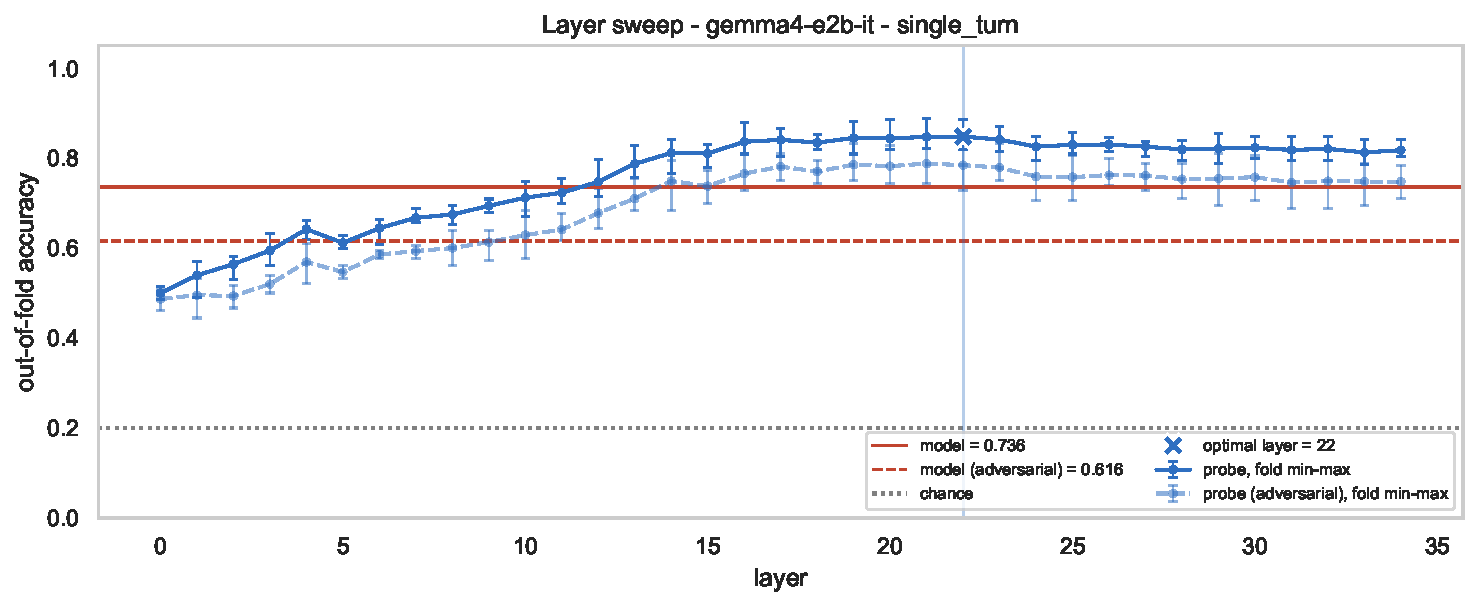
\includegraphics[width=0.85\textwidth]{images/models/gemma4-e2b-it_single_turn_layers.pdf}
    \caption[Layer sweep, gemma4-e2b-it, single-turn]{Layer sweep, gemma4-e2b-it, single-turn.}
    \label{fig:appendix-gemma4-e2b-it-single-layers}
\end{figure}

\begin{figure}[H]
    \centering
    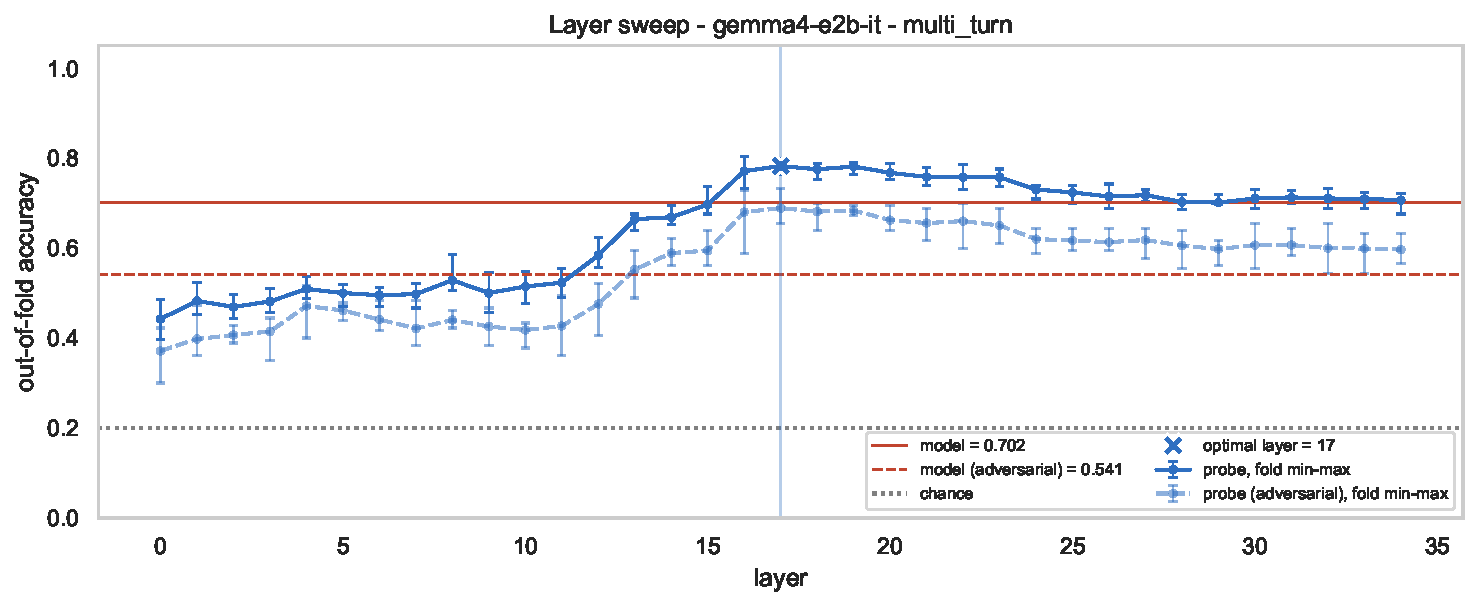
\includegraphics[width=0.85\textwidth]{images/models/gemma4-e2b-it_multi_turn_layers.pdf}
    \caption[Layer sweep, gemma4-e2b-it, multi-turn]{Layer sweep, gemma4-e2b-it, multi-turn.}
    \label{fig:appendix-gemma4-e2b-it-multi-layers}
\end{figure}

\section{Qwen3 4B Instruct 2507}
\label{sec:appendix-layer-sweep-qwen3-4b}

\begin{figure}[H]
    \centering
    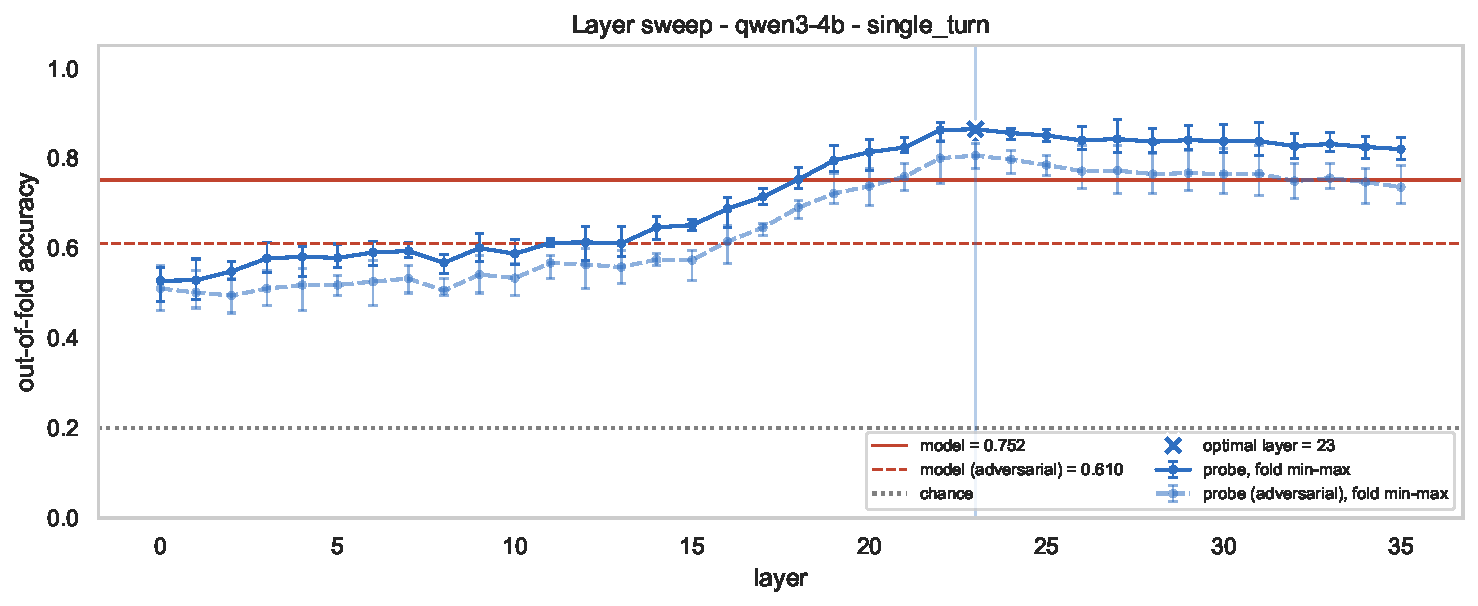
\includegraphics[width=0.85\textwidth]{images/models/qwen3-4b_single_turn_layers.pdf}
    \caption[Layer sweep, qwen3-4b, single-turn]{Layer sweep, qwen3-4b, single-turn.}
    \label{fig:appendix-qwen3-4b-single-layers}
\end{figure}

\begin{figure}[H]
    \centering
    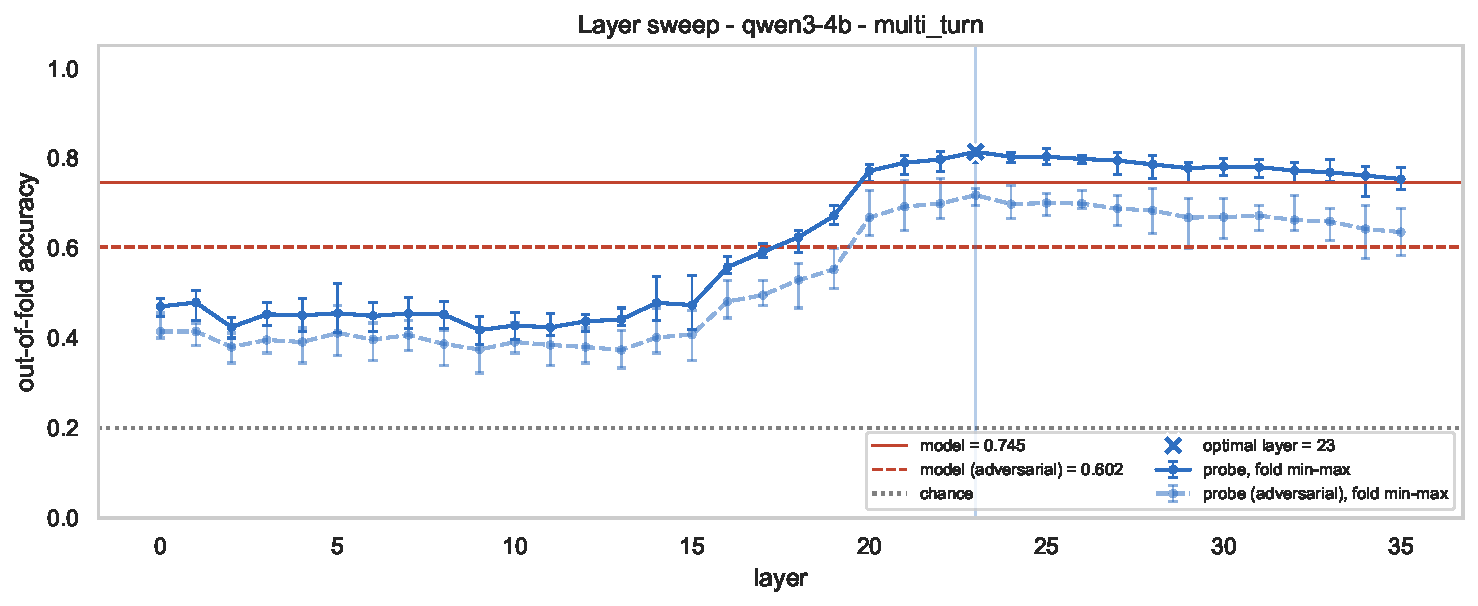
\includegraphics[width=0.85\textwidth]{images/models/qwen3-4b_multi_turn_layers.pdf}
    \caption[Layer sweep, qwen3-4b, multi-turn]{Layer sweep, qwen3-4b, multi-turn.}
    \label{fig:appendix-qwen3-4b-multi-layers}
\end{figure}

\section{Qwen3 8B}
\label{sec:appendix-layer-sweep-qwen3-8b}

\begin{figure}[H]
    \centering
    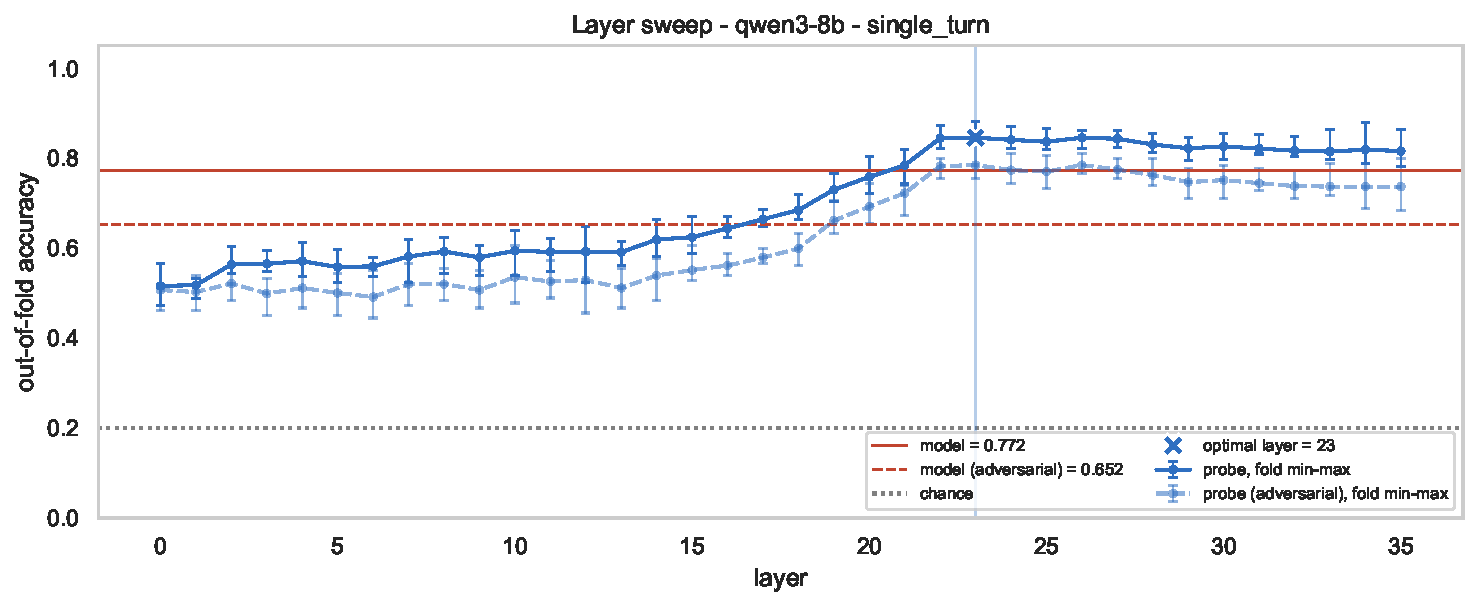
\includegraphics[width=0.85\textwidth]{images/models/qwen3-8b_single_turn_layers.pdf}
    \caption[Layer sweep, qwen3-8b, single-turn]{Layer sweep, qwen3-8b, single-turn.}
    \label{fig:appendix-qwen3-8b-single-layers}
\end{figure}

\begin{figure}[H]
    \centering
    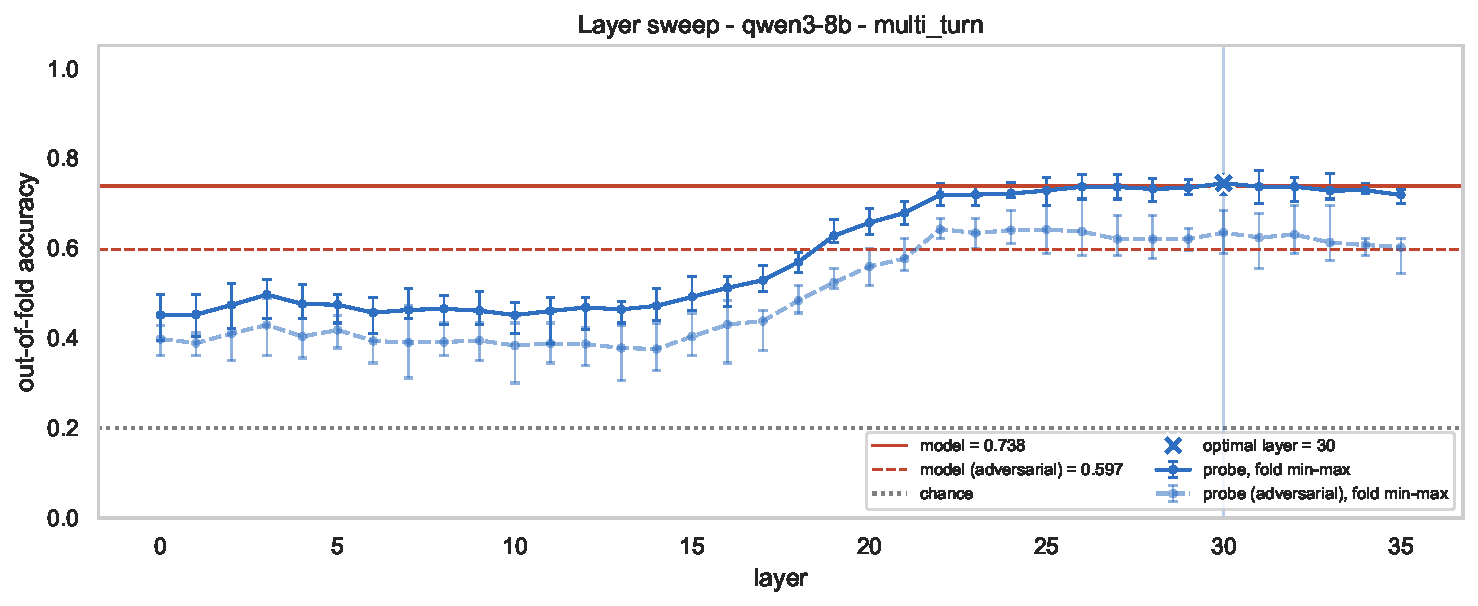
\includegraphics[width=0.85\textwidth]{images/models/qwen3-8b_multi_turn_layers.pdf}
    \caption[Layer sweep, qwen3-8b, multi-turn]{Layer sweep, qwen3-8b, multi-turn.}
    \label{fig:appendix-qwen3-8b-multi-layers}
\end{figure}

\section{Gemma 4 12B IT}
\label{sec:appendix-layer-sweep-gemma4-12b-it}

\begin{figure}[H]
    \centering
    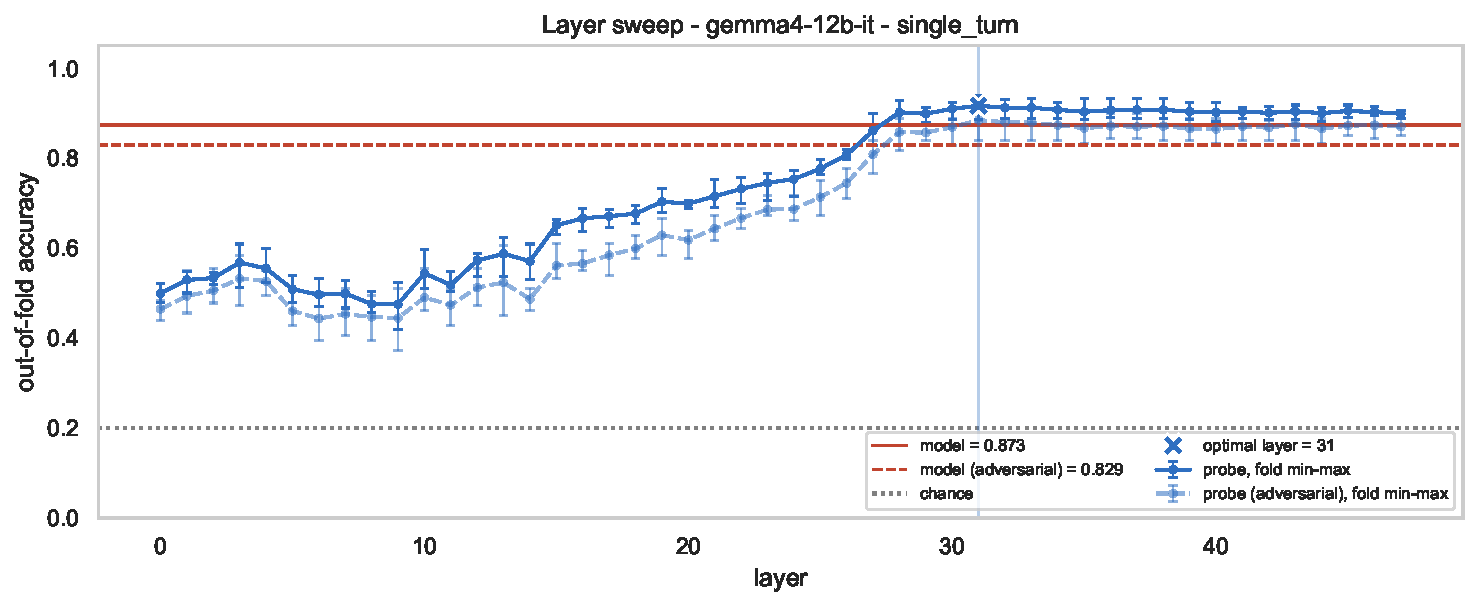
\includegraphics[width=0.85\textwidth]{images/models/gemma4-12b-it_single_turn_layers.pdf}
    \caption[Layer sweep, gemma4-12b-it, single-turn]{Layer sweep, gemma4-12b-it, single-turn.}
    \label{fig:appendix-gemma4-12b-it-single-layers}
\end{figure}

\begin{figure}[H]
    \centering
    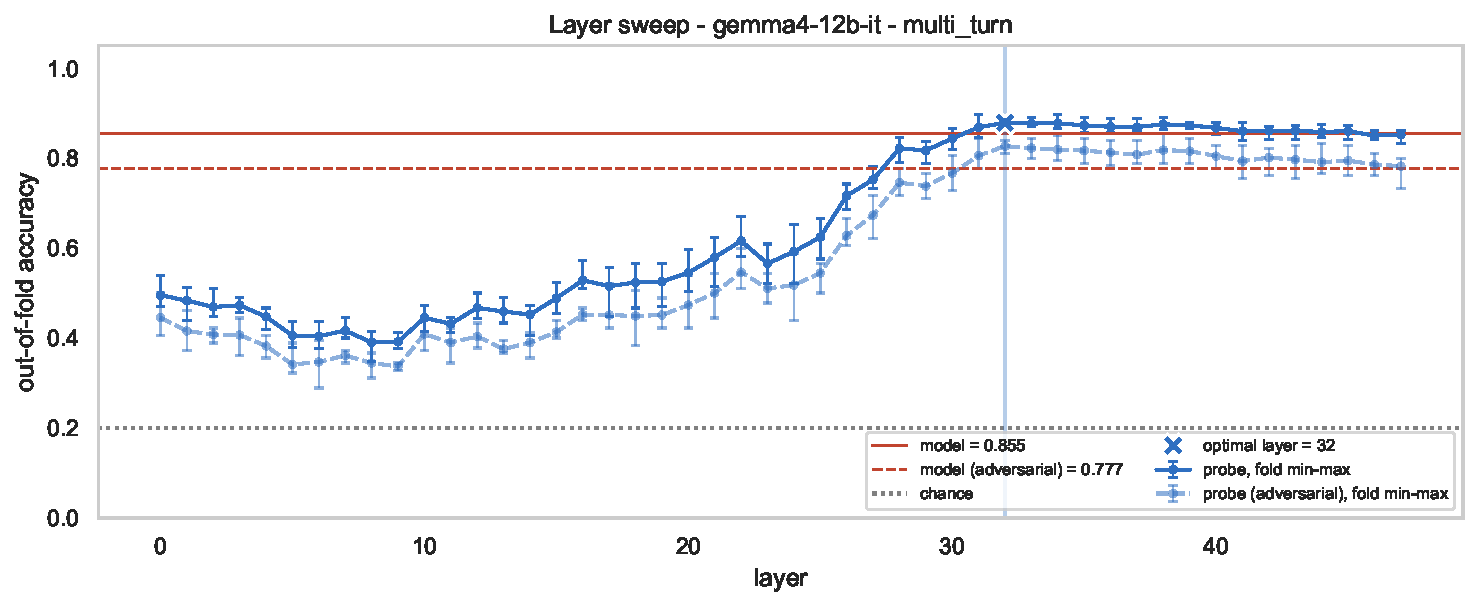
\includegraphics[width=0.85\textwidth]{images/models/gemma4-12b-it_multi_turn_layers.pdf}
    \caption[Layer sweep, gemma4-12b-it, multi-turn]{Layer sweep, gemma4-12b-it, multi-turn.}
    \label{fig:appendix-gemma4-12b-it-multi-layers}
\end{figure}

\section{Gemma 4 26B A4B IT}
\label{sec:appendix-layer-sweep-gemma4-26b-a4b-it}

\begin{figure}[H]
    \centering
    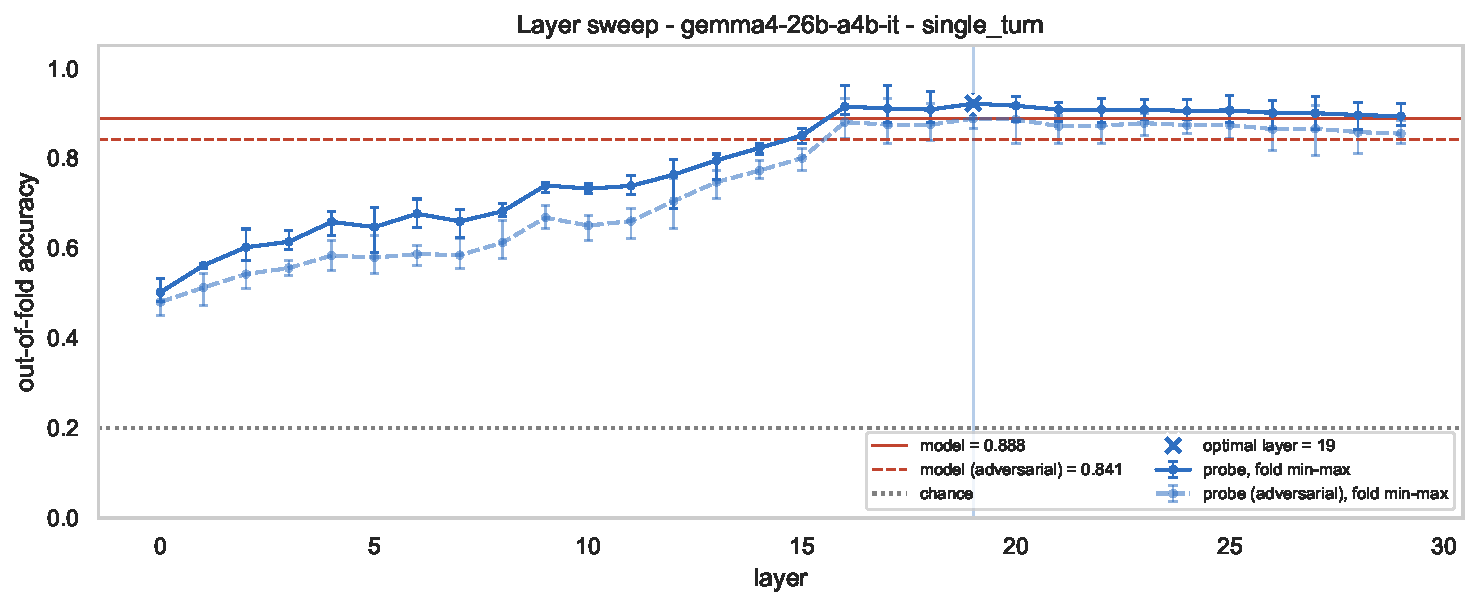
\includegraphics[width=0.85\textwidth]{images/models/gemma4-26b-a4b-it_single_turn_layers.pdf}
    \caption[Layer sweep, gemma4-26b-a4b-it, single-turn]{Layer sweep, gemma4-26b-a4b-it, single-turn.}
    \label{fig:appendix-gemma4-26b-a4b-it-single-layers}
\end{figure}

\begin{figure}[H]
    \centering
    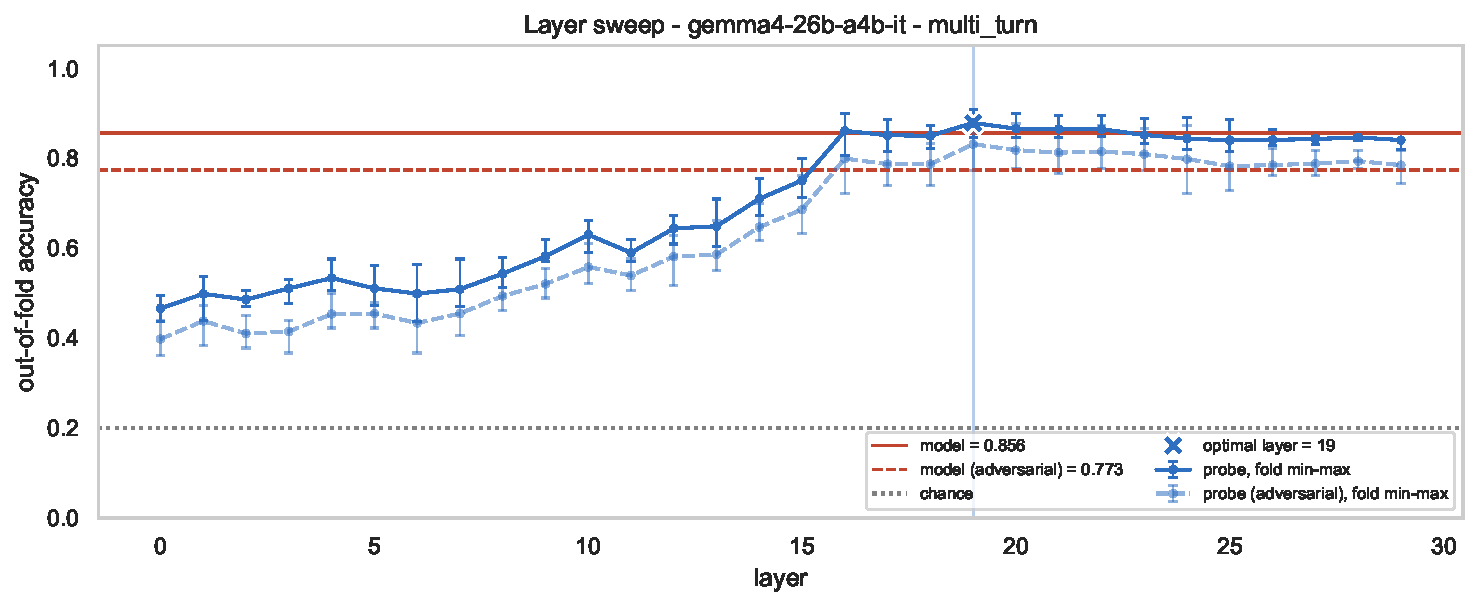
\includegraphics[width=0.85\textwidth]{images/models/gemma4-26b-a4b-it_multi_turn_layers.pdf}
    \caption[Layer sweep, gemma4-26b-a4b-it, multi-turn]{Layer sweep, gemma4-26b-a4b-it, multi-turn.}
    \label{fig:appendix-gemma4-26b-a4b-it-multi-layers}
\end{figure}

\section{Llama 3.3 70B Instruct}
\label{sec:appendix-layer-sweep-llama33-70b}

\begin{figure}[H]
    \centering
    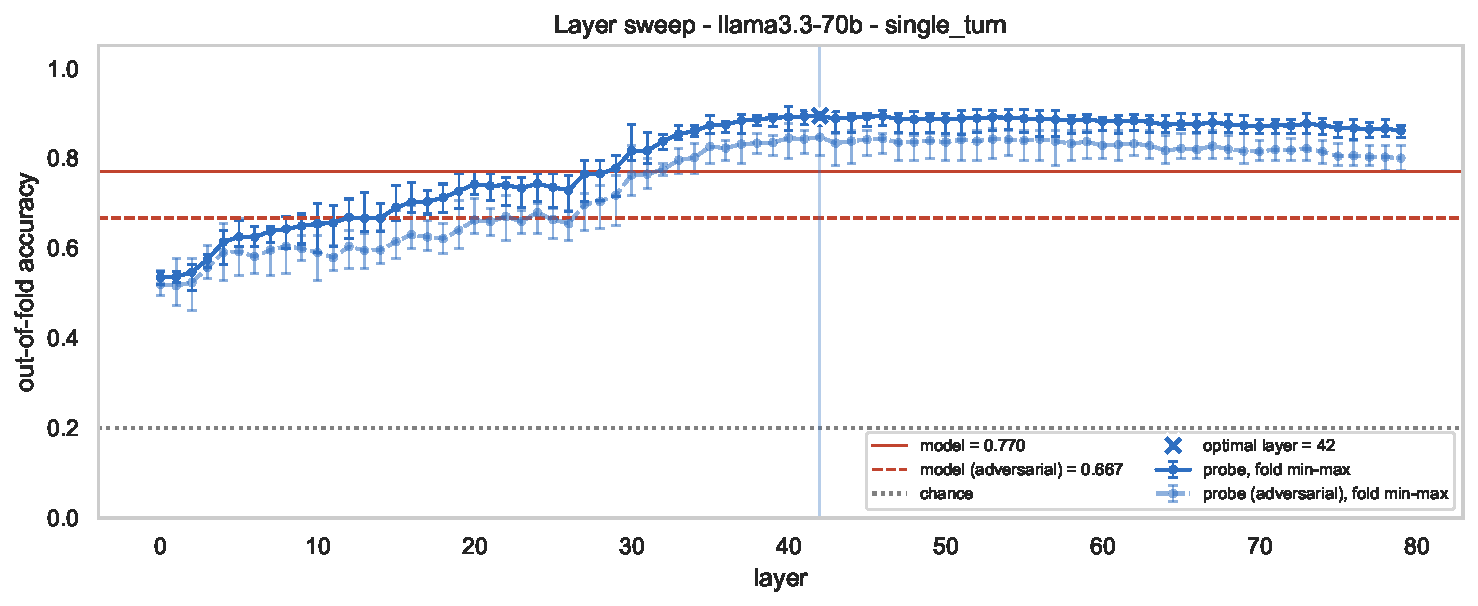
\includegraphics[width=0.85\textwidth]{images/models/llama33-70b_single_turn_layers.pdf}
    \caption[Layer sweep, llama3.3-70b, single-turn]{Layer sweep, llama3.3-70b, single-turn.}
    \label{fig:appendix-llama33-70b-single-layers}
\end{figure}

\begin{figure}[H]
    \centering
    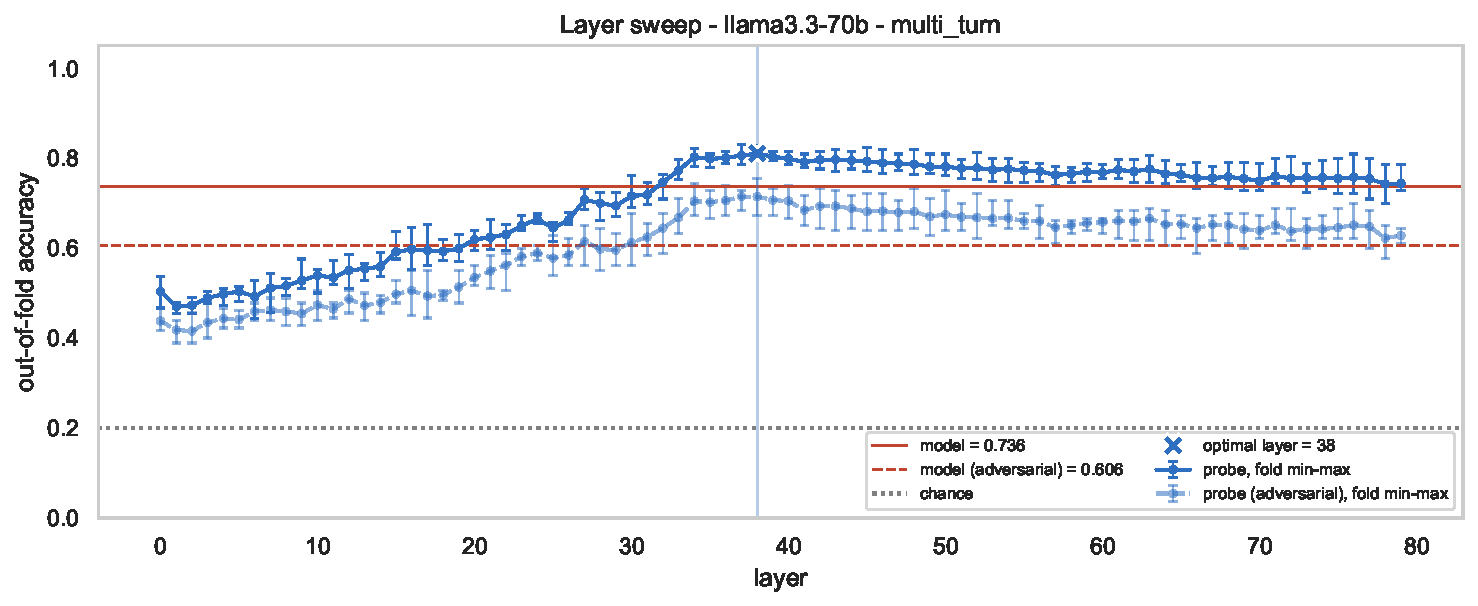
\includegraphics[width=0.85\textwidth]{images/models/llama33-70b_multi_turn_layers.pdf}
    \caption[Layer sweep, llama3.3-70b, multi-turn]{Layer sweep, llama3.3-70b, multi-turn.}
    \label{fig:appendix-llama33-70b-multi-layers}
\end{figure}

\section{Qwen2.5 72B Instruct}
\label{sec:appendix-layer-sweep-qwen25-72b}

\begin{figure}[H]
    \centering
    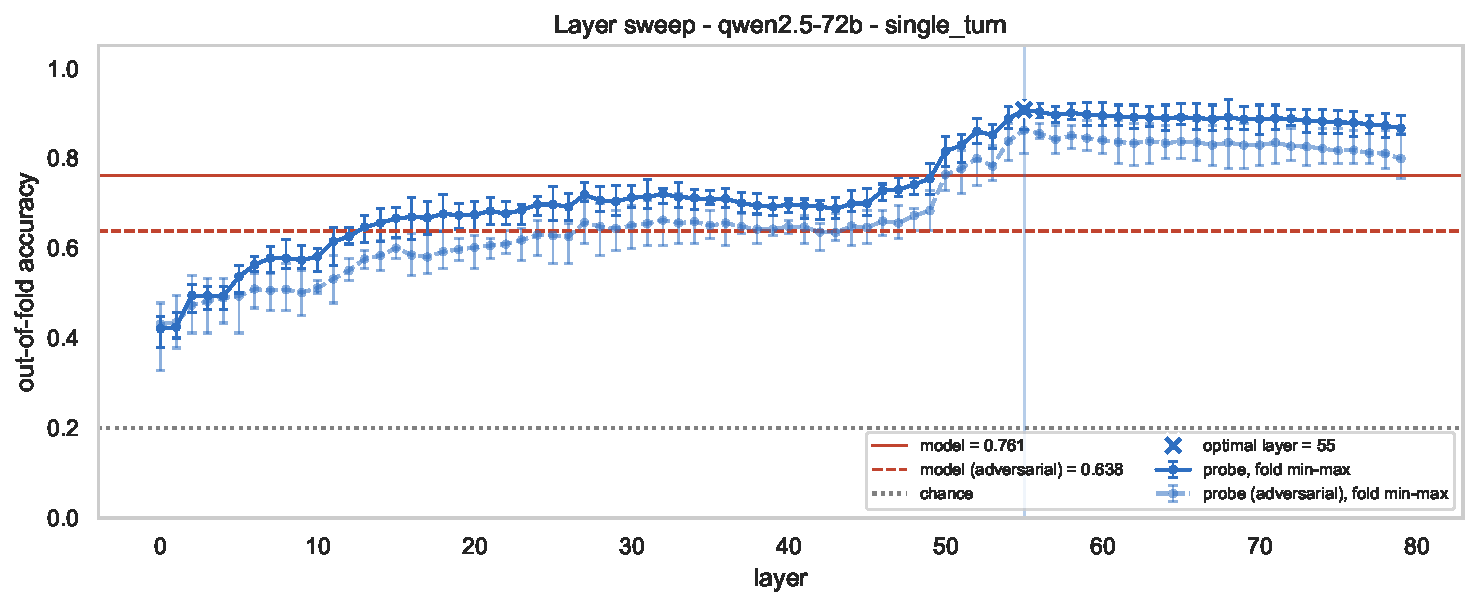
\includegraphics[width=0.85\textwidth]{images/models/qwen25-72b_single_turn_layers.pdf}
    \caption[Layer sweep, qwen2.5-72b, single-turn]{Layer sweep, qwen2.5-72b, single-turn.}
    \label{fig:appendix-qwen25-72b-single-layers}
\end{figure}

\begin{figure}[H]
    \centering
    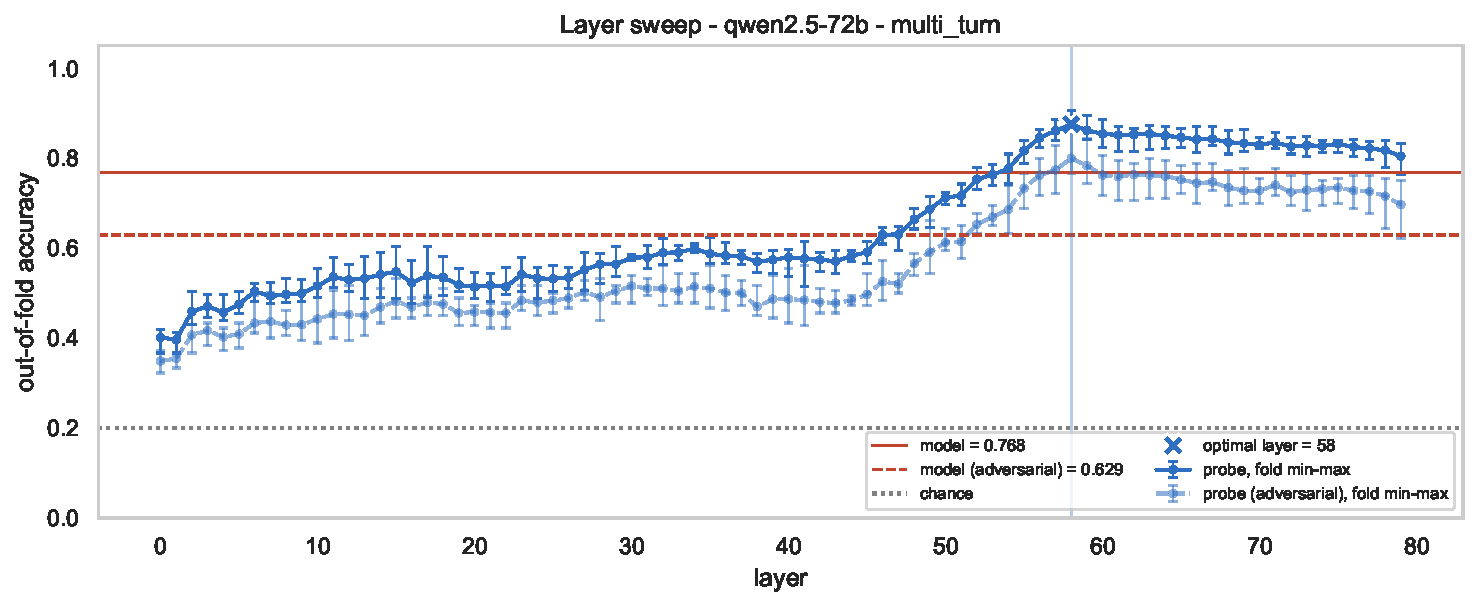
\includegraphics[width=0.85\textwidth]{images/models/qwen25-72b_multi_turn_layers.pdf}
    \caption[Layer sweep, qwen2.5-72b, multi-turn]{Layer sweep, qwen2.5-72b, multi-turn.}
    \label{fig:appendix-qwen25-72b-multi-layers}
\end{figure}

\section{GPT-OSS 20B}
\label{sec:appendix-layer-sweep-gpt-oss-20b}

\begin{figure}[H]
    \centering
    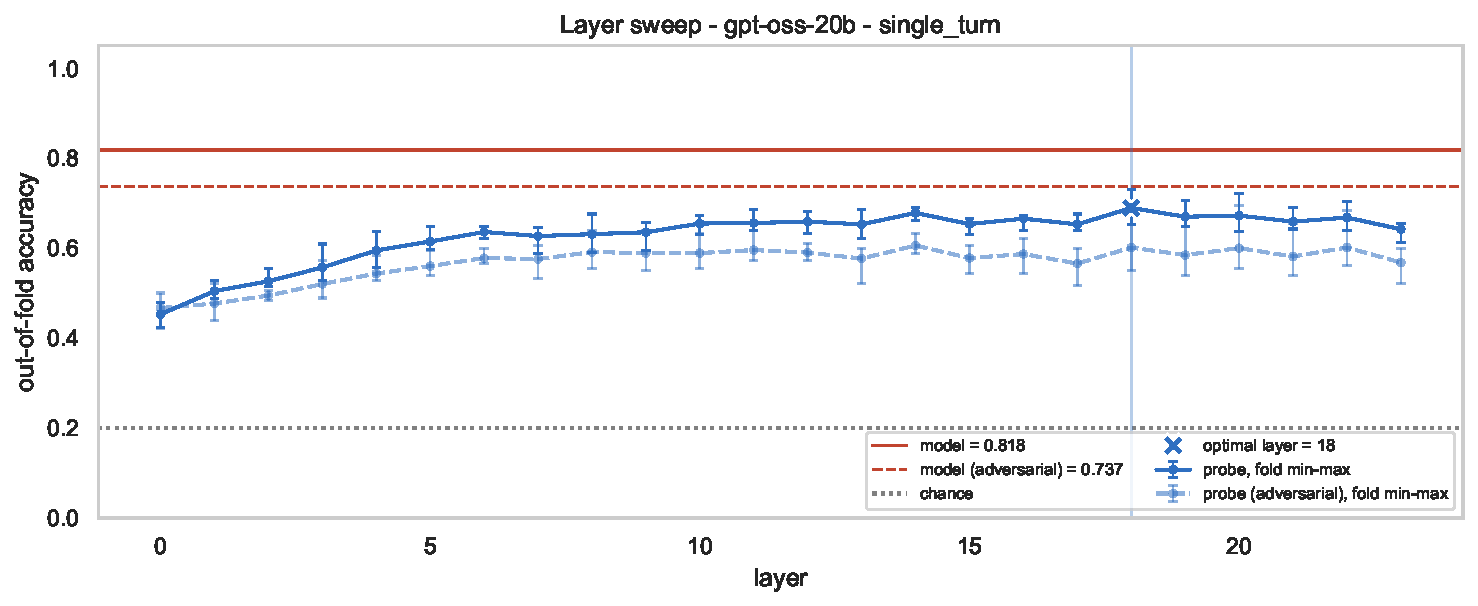
\includegraphics[width=0.85\textwidth]{images/models/gpt-oss-20b_single_turn_layers.pdf}
    \caption[Layer sweep, gpt-oss-20b, single-turn]{Layer sweep, gpt-oss-20b, single-turn.}
    \label{fig:appendix-gpt-oss-20b-single-layers}
\end{figure}

\begin{figure}[H]
    \centering
    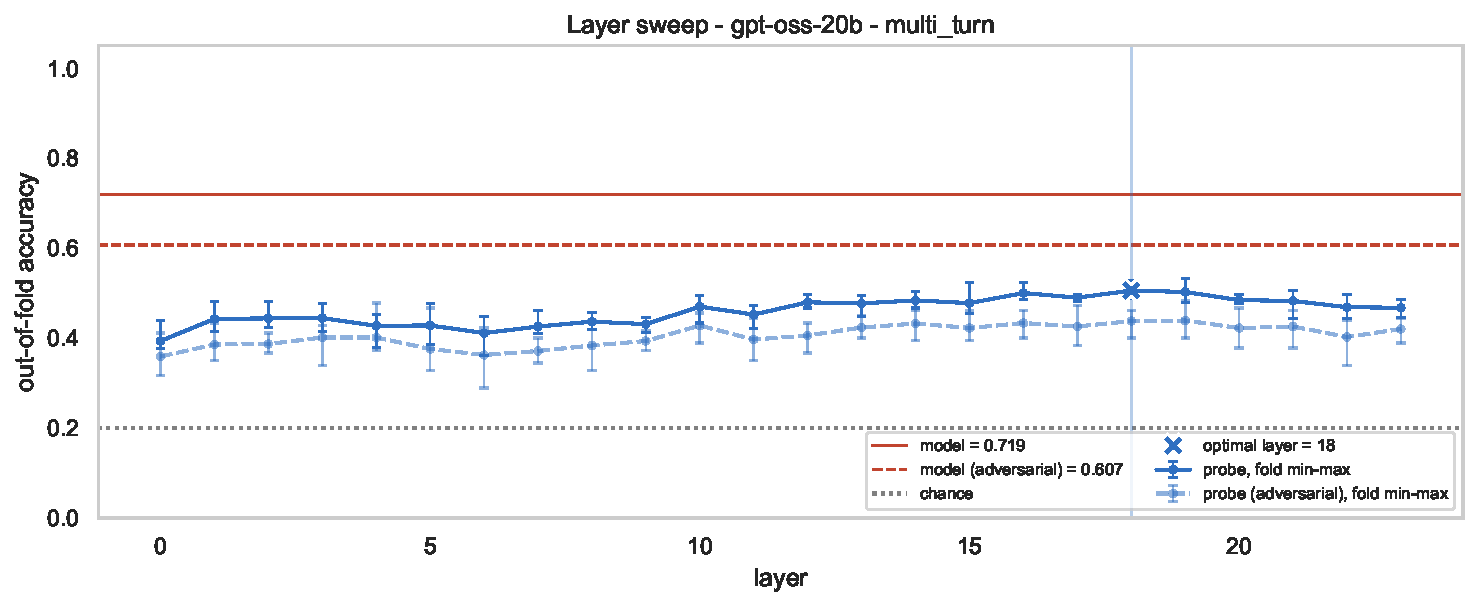
\includegraphics[width=0.85\textwidth]{images/models/gpt-oss-20b_multi_turn_layers.pdf}
    \caption[Layer sweep, gpt-oss-20b, multi-turn]{Layer sweep, gpt-oss-20b, multi-turn.}
    \label{fig:appendix-gpt-oss-20b-multi-layers}
\end{figure}

\begin{figure}[H]
    \centering
    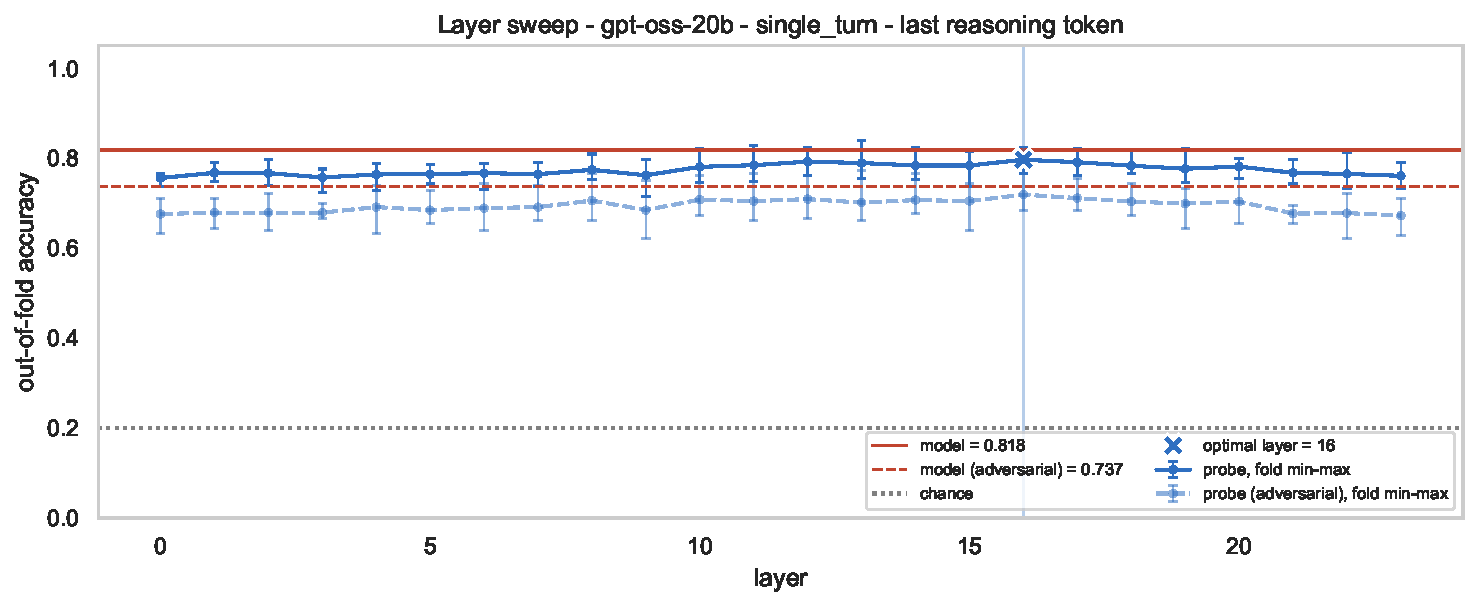
\includegraphics[width=0.85\textwidth]{images/models/gpt-oss-20b_single_turn_reasoning_layers.pdf}
    \caption[Layer sweep, gpt-oss-20b, single-turn, last reasoning token]{Layer sweep, gpt-oss-20b, single-turn, hidden states at the last reasoning token (Section~\ref{subsec:ch8-gpt-oss-reasoning}).}
    \label{fig:appendix-gpt-oss-20b-single-reasoning-layers}
\end{figure}


\backmatter

\bibliographystyle{plain_\languagename}
\bibliography{thud}

\end{document}
